\documentclass[draft]{wzuthesis} % 不填充空白页。如果需要双面打印版，请注释掉本行并启用下一行
% \documentclass[print-both-sides]{scutthesis} % 使用双面打印版（填充额外空白页以保证每一章开头都在奇数页）
\usepackage{mathptmx}
\usepackage{enumitem}
\usepackage{bicaption}
\usepackage{subcaption} 
\usepackage{caption}
\usepackage{amsmath}
% 必须导入的包（放在文档开头）
\usepackage{multirow}
\usepackage{array}

\usepackage[utf8]{inputenc}
\usepackage{booktabs}   % 提供更美观的学术线条 \toprule, \midrule, \bottomrule
\usepackage{tabularx}   % 自动换行列

\usepackage{pdflscape} % 最优横版宏包

\bicaptionsetup[figure]{}{name=Fig.}
\bicaptionsetup[table]{}{name=Table}
\setlength{\headheight}{13pt}

%\setmainfont{Times New Roman}[
%  Path = ./fonts/,
%  Extension = .ttf,
%  UprightFont = times,
%  BoldFont = timesbd,
%  ItalicFont = timesi,
%  BoldItalicFont = timesbi
%]

\setmainfont{Times New Roman}[
UprightFont = *,
BoldFont = * Bold,
ItalicFont = * Italic,
BoldItalicFont = * Bold Italic
]

%%===============论文信息=============================
\ctitle{面向医学数据集的特征选择算法研究} 
                                % 中文题目
\etitle{Research on Feature Selection Algorithms for Disease Prediction on Medical Data}                     % 英文题目

\cauthor{邱\ 从\ 波}            % 作者姓名
\fen{TP391.4}                  % 分类号
\udc{004.8}                    % UDC
\id{23451350028}               % 学号
\mi{公开}                       % 密级
\xwlx{学术型}                   %学位类型
\pylx{全日制统招研究生}         % 培养类型
\cmajor{计算机科学与技术}       % 专业名称
\cclass{智能计算与数据挖掘}              % 研究方向
\cmentor{黄长城（教授） 陈慧灵（教授）} % 指导老师
\cdata{2026年3月1日} %完成时间
\blindcode{} % 盲审代码
%%===================================================
% \def\blind{}       % 盲审版把这条注释打开



\cabstract{
随着生物信息学的快速发展，病理数据的维度迅速增长，高维医疗数据已成为医学研究与临床实践的核心数据基础。但对高维医疗数据的有效分析却面临着特征数量致使计算复杂度剧增、机器学习模型性能劣化、计算资源消耗大等严峻挑战。高维医学特征的有效解析，已成为医学研究与临床实践的关键技术问题。
特征选择作为高维数据处理的核心技术，通过筛选原始数据中最具相关性与代表性的特征，从而提高机器学习模型性能，降低计算消耗。元启发式算法作为一种有效手段曾被广泛用于特征选择，但是朴素启发式算法面临着诸多问题，诸如开发与探索的平衡问题，早熟收敛问题等。

为了解决元启发式算法的这些问题，本论文提出了二种改进型的启发式算法，通过引入针对性的改进机制，解决了两种算法原本的弊端和面对高维医学数据时的不足。

在第三章中，本文针对雾凇算法（RIME）的不足，提出一种改进的雾凇算法（IRIME），它结合信息熵评估策略、随机重启机制和拉格朗日插值方法来克服这些局限。信息熵评估策略通过对特征动态加权增强种群多样性，随机重启机制防止过早收敛，拉格朗日插值方法通过逼近全局最优解加速收敛。在 CEC 2017 测试集上的大量对比实验表明，IRIME 的性能不仅优于原算法RIME，而且优于其他 7 种知名算法。在 30 维度和 50 维度的弗里德曼（Friedman）检验中分别排名 1.31 和 1.21 ，大幅领先于其他 8 种算法，其收敛速度更快且稳定性更高。在随后的特征选择实验中，我们宽泛地选取了 8 个中低维度数据集和 4 个高维数据集进行实验，这些数据集均来自真实的临床数据，涵盖多样的数据特性。实验结果显示，IRIME 在适应度值、准确率以及特征子集大小方面，均保持领先地位。特别在高维数据集 ALLAML 和 TOX-171 上，IRIME 分别以 100\% 和 88.24\% 的分类准确率夺得第一。经实验验证，IRIME 方法在医学数据特征选择场景下展现出优异的实用价值，为医学数据特征选择领域补充了一种可靠的技术手段。

在第四章中，为解决原始哈里斯鹰优化算法（HHO）在迭代过程中易陷入局部最优、种群多样性下降、后期收敛精度不足等问题，提出一种融合多策略的改进哈里斯鹰优化算法（IHHO）。本文首先引入经验互益策略，整合历史种群的有效搜索信息，增强种群个体间的信息交互能力，提升算法跳出局部最优的潜能；其次设计能量自适应扰动策略，依据猎物逃逸能量动态调整扰动比例，实现全局广域探索与局部精准开发的动态平衡；最后提出精英方差引导开发策略，通过计算精英个体的逐维方差确定局部搜索步长，解决算法后期搜索的局部振荡问题，提升局部优化精度。在 CEC 2020 标准测试函数集，将其与原始 HHO 及 另外 5 种经典群智能优化算法进行对比实验。实验结果显示，IHHO 的弗里德曼（Friedman）平均排名为 1.43，显著优于对比算法。将 IHHO 算法应用于高维特征选择问题，选取 8 个高维数据集开展实验，从适应度值、分类准确率与特征压缩效果等维度进行验证。结果显示，IHHO 在 Breast、CNS、Leukemia 等多数高维数据集中取得了更低的平均适应度值与更高的分类准确率，部分数据集分类准确率达到100\%，所选特征子集兼具良好的判别性与泛化性，有效实现了高维特征的精准筛选与冗余特征消除。以上实验表明，所提多策略改进方法能显著提升哈里斯鹰优化算法的综合性能，并在连续函数优化与高维特征选择领域均具有良好的应用效果与推广价值。
}
\ckeywords{元启发算法，雾凇算法，哈里斯鹰优化算法，特征选择，高维数据集}

\eabstract{
With the rapid development of bioinformatics, the dimensionality of pathological data has grown exponentially, making high-dimensional medical data the core foundation for medical research and clinical practice. However, effective analysis of such data faces severe challenges, including a sharp increase in computational complexity, degradation of machine learning model performance, and excessive consumption of computational resources. Effectively parsing high-dimensional medical features has become a critical technical issue in both research and clinical settings.

Feature selection, a core technique in high-dimensional data processing, enhances machine learning performance and reduces computational overhead by screening the most relevant and representative features. While meta-heuristic algorithms have been widely adopted for feature selection, vanilla versions suffer from issues such as the imbalance between exploration and exploitation, as well as premature convergence.

To address these limitations, this thesis proposes two improved heuristic algorithms. By introducing targeted optimization mechanisms, these methods overcome the inherent drawbacks of the original algorithms and their deficiencies when handling high-dimensional medical data.

In Chapter 3, an Improved RIME (IRIME) is proposed to address the shortcomings of the original RIME algorithm. IRIME integrates an information entropy evaluation strategy, a random restart mechanism, and Lagrange interpolation to overcome these limitations. The information entropy strategy enhances population diversity through dynamic feature weighting; the random restart mechanism prevents premature convergence; and the Lagrange interpolation method accelerates convergence by approximating the global optimal solution. Extensive comparative experiments on the CEC 2017 test suite demonstrate that IRIME outperforms the original RIME and seven other well-known algorithms. In the Friedman test, IRIME ranked 1.31 and 1.21 for 30 and 50 dimensions respectively, significantly leading the other eight algorithms with faster convergence and higher stability. Subsequent feature selection experiments using eight low-to-medium dimensional datasets and four high-dimensional datasets-all derived from real clinical data-showed that IRIME maintains a leading position in fitness values, accuracy, and feature subset size. Notably, on the high-dimensional datasets ALLAML and TOX-171, IRIME achieved first place with classification accuracies of 100\% and 88.24\%, respectively. Experimental results verify that the IRIME method possesses excellent practical value for medical feature selection.

In Chapter 4, an Improved Harris Hawks Optimization (IHHO) algorithm incorporating multiple strategies is proposed to resolve issues in the original HHO, such as susceptibility to local optima, declining population diversity, and insufficient convergence precision in later stages. First, an experience mutual-benefit strategy is introduced to integrate effective search information from historical populations, enhancing information interaction and the potential to escape local optima. Second, an energy adaptive perturbation strategy is designed to dynamically adjust perturbation ratios based on prey escape energy, achieving a balance between global exploration and local exploitation. Finally, an elite variance-guided exploitation strategy is proposed to determine local search step sizes by calculating the dimensional variance of elite individuals, addressing local oscillations and improving precision. Comparative experiments on the CEC 2020 benchmark functions against the original HHO and five other classic swarm intelligence algorithms show that IHHO achieved a Friedman mean rank of 1.43, significantly outperforming competitors. When applied to high-dimensional feature selection across eight datasets, IHHO achieved lower mean fitness values and higher classification accuracies in most sets (such as Breast, CNS, and Leukemia), with some reaching 100\% accuracy. The selected feature subsets exhibit strong discriminative power and generalization, effectively achieving precise screening and redundancy elimination. These results indicate that the proposed multi-strategy improvements significantly enhance the comprehensive performance of HHO, offering high application value in both continuous function optimization and high-dimensional feature selection.
}
% 英文文关键词(每个关键词之间用,分开, 最后一个关键词不打标点符号。)
\ekeywords{meta-heuristic, RIME, Harris Hawks Optimization, feature selection, high-dimensional datasets}

\begin{document}
% 论文前置部分

\frontmatter
\makefirstpage
% 如果不需要图、表目录前往cls文件中将相应的注释掉

% 论文主体部分
\mainmatter
\chapter{绪论}
\section {研究背景}
生物信息学的快速发展推动病理数据维度呈指数级增长，高维医疗数据已成为医学研究与临床实践的核心数据基础，其丰富信息为精准医疗诊断、个性化治疗提供了重要支撑。但高维医疗数据的分析处理面临显著挑战：特征冗余引发维度灾难，致使计算复杂度剧增、模型性能劣化、数据分析难度提升，且需消耗大量计算资源；同时数据过拟合风险显著升高。

高维医学特征的有效解析，已成为医学研究与临床实践的关键技术问题。特征选择作为高维数据处理的核心技术，通过筛选原始数据中最具相关性与代表性的特征，在生物信息学及医学研究中可实现疾病生物标志物、基因识别、诊断辅助、治疗结局预测及新型治疗靶点挖掘。特征选择对于提高机器学习模型性能至关重要，元启发式算法作为一种有效手段曾被广泛用于特征选择。但是朴素启发式算法面临着诸多问题，诸如开发与探索的平衡问题，早熟收敛问题，和参数敏感性等。本论文直接利用这些高维医学数据进行疾病诊断、预后预测等任务时，不仅会产生高昂的计算成本，还会因特征空间的维数灾难导致数据稀疏性加剧，严重影响模型的泛化能力与诊断可靠性。


特征选择旨在从海量数据中提取有效信息，而机器学习与人工智能的现代化发展为医学数据分析提供了强大工具。但在医学数据的模型训练过程中，原始高维特征集中不仅包含与疾病诊断、病理分析相关的关键信息，还混杂着大量冗余特征，如高度相关的临床指标、无生物学意义的噪声特征和无关特征。这些冗余与无关特征不仅会大幅增加计算开销、延长模型训练周期，更会干扰模型对核心医学规律的学习，导致诊断准确率下降、假阳性率升高，这在生死攸关的医学场景中可能引发严重后果。因此，高维医学数据的特征选择已成为机器学习在医学领域落地应用的关键预处理技术，其核心目标是在剔除冗余与无关特征的同时，保留最具医学诊断价值、最能反映病理生理机制的核心特征子集。


特征选择方法可分为过滤式、嵌入式、封装式三类\overcite {maldonado2022review}，三类方法的差异体现在分类器与特征选择流程的融合方式上。过滤式方法\overcite {babalik2024binary} 采用相关性、互信息等统计准则完成特征筛选\overcite {pengmutation2005}，该类方法简单高效，能够有效缩减特征子集，但灵活性不足，通常无法解决医学高维数据中特征间复杂的非线性冗余问题；嵌入式方法\overcite {hussien2019s};\overcite {embedded1} 将特征选择嵌入分类器训练过程，提升了算法交互性，但也增加了模型训练与参数调优的复杂度，在医学数据的小样本场景下易出现过拟合；封装式方法\overcite {gonzalez2019new} 将特征选择转化为搜索问题，通过模型性能指标评估特征子集的优劣。

元启发式算法凭借其天然的全局优化特性，与特征选择任务的核心需求高度适配，能够通过模拟自然群体行为高效筛选出低冗余、高判别力的特征子集。为实现复杂高维数据的有效处理，科研人员围绕优化算法的搜索策略展开了大量改进研究，通过融合多策略、增强种群多样性、动态平衡探索与开发过程等方式提升算法优化性能，进而提出了一系列基于元启发式算法的特征选择方法。

然而，针对医学高维数据集的特征选择任务，现有元启发式算法面临的挑战更为突出：医学数据的高维性使得搜索空间呈指数级爆炸式增长，加剧了数据稀疏性与基于距离的求解难题；同时，医学特征往往具有强相关性、非线性耦合等特点，导致算法更易陷入局部最优，难以挖掘到真正具有临床意义的核心特征子集。具体而言，元启发式算法在医学高维特征选择中面临双重核心挑战：一是迭代过程中解的多样性持续衰减，削弱全局优化能力，无法突破医学特征空间中的局部最优陷阱；二是算法性能对人工调优的参数高度敏感，导致性能波动较大，而医学数据的异质性进一步放大了参数依赖性带来的负面影响，降低了算法在不同医学场景下的泛化能力。


更值得注意的是，在医学数据集的特征选择任务中，启发式算法普遍面临的四大核心难题表现得更为尖锐：
(1) 早熟收敛与局部最优：医学高维特征空间的复杂性使得算法更易收敛至次优解，筛选出的特征子集可能包含大量冗余信息，无法准确反映疾病的病理生理机制，影响临床应用价值；
(2) 稳定性差：算法结果对初始种群配置、随机种子高度敏感，重复实验的结果波动显著，而医学诊断对模型的稳定性与可靠性要求极高，波动过大的特征选择结果会严重影响诊断一致性；
(3) 参数依赖性：算法依赖大量超参数调优，不仅引入主观偏差，还因医学数据的特异性导致最优参数难以迁移，降低了算法在不同疾病数据集、不同医疗机构数据集中的泛化能力；
(4) 可扩展性受限：医学超高维场景下搜索空间呈爆炸式增长，算法无法在合理时间内完成收敛，难以满足临床实时诊断的需求。


尽管不少启发式方法在通用数据集上取得良好效果，但在医学高维数据场景中仍存在诸多不足：例如参数设置复杂、泛化能力弱、鲁棒性差，且难以平衡 “特征降维幅度” 与 “临床诊断精度” 过度降维可能丢失关键医学特征，导致诊断漏诊，而降维不足则无法解决维数灾难问题。 NFL 定理\overcite {wolpert1997no} 从理论上证明：不存在可最优求解所有特征选择问题的通用算法，这一结论在医学数据领域尤为显著：不同疾病的病理机制差异、数据采集技术的多样性，使得单一算法难以适配所有医学高维特征选择场景，亟需针对医学数据的特殊性设计专用优化算法。

% 医学高维特征选择的优劣直接关系到疾病诊断的准确性、预后评估的可靠性以及临床决策的科学性，其研究具有重要的理论意义与临床应用价值。

% 据此，本文提出两种多策略融合改进算法：

% （1）改进型雾凇算法（IRIME），该算法融合三大核心策略：信息熵评价策略、随机重启机制、拉格朗日插值法。信息熵评价策略通过对特征动态加权，提升种群多样性与全局探索能力，适配医学特征的复杂分布；随机重启机制通过重新初始化低适应度个体避免算法停滞，有效突破医学高维空间的局部最优陷阱；拉格朗日插值法通过逼近全局最优解加速算法收敛，满足医学数据处理的效率需求。基于 CEC2017 测试集的实验表明，IRIME 性能优于七种主流算法；在  8 个中低维数据集和 4 个高维医学数据集上，IRIME 以最小特征冗余实现了高精度分类，为临床诊断提供了更具针对性的特征子集；消融实验进一步验证了三种策略的协同有效性。

% （2）融合多策略的改进哈里斯鹰优化算法（IHHO）。该算法首先引入经验互益策略，整合历史种群的有效搜索信息，增强种群个体间的信息交互能力，提升算法跳出医学高维特征空间局部最优的潜能；其次设计能量自适应扰动策略，依据猎物逃逸能量动态调整扰动比例，实现全局广域探索与局部精准开发的动态平衡，适配医学特征的强相关性与非线性特点；最后提出精英方差引导开发策略，通过计算精英个体的逐维方差确定局部搜索步长，解决算法后期搜索的局部振荡问题，提升局部优化精度，确保筛选出的特征子集具有稳定的临床诊断价值。通过时间复杂度分析明确了 IHHO 的计算成本，同时给出了算法的完整实现步骤，为医学高维特征选择提供了高效可行的解决方案。

\section {国内外研究现状}
% 优化的核心目标是在各类理论研究与工程应用中，为特定问题求解最优解决方案。随着实际问题复杂程度的持续提升，各领域对优化技术的性能要求日益严苛，高维数据场景下的特征选择问题尤为突出，其 NP 难特性与爆炸式增长的搜索空间，对优化算法的全局探索能力、收敛效率与鲁棒性提出了更高挑战。

近年来，启发式算法已成为机器学习领域的核心优化工具，尤其适用于求解具备大解空间与 NP 难特性的复杂优化问题\overcite {karimi2022machine}。这类算法依托创新搜索策略生成近似最优解，在求解效率与场景适应性上普遍优于传统优化方法。按照启发来源划分，启发式算法可归为四大类别\overcite {ss2022nature}：进化算法、群智能算法、物理启发算法与人类行为启发算法\overcite {zhao2024triangulation}。
进化算法受生物进化规律启发，通过交叉、变异、选择、淘汰等操作迭代优化候选解种群，迭代过程中剔除低适应度个体、保留并进化高适应度个体，进而持续提升种群整体适应性。遗传算法\overcite {liao2023genetic}是最具代表性的进化计算方法，同类算法还包括差分进化算法\overcite {song2023dynamic}。群智能算法通过模拟简单个体间的局部交互与自组织行为求解复杂问题，实现群体层面的涌现智能，经典算法包含蚁群优化算法\overcite {wang2021ant}、粒子群优化算法\overcite {du2023orderly}，以及近年来提出的麻雀搜索算法\overcite {SSAxue2020novel}、秃鹰搜索算法\overcite {BESalsattar2020novel}）与海鸥优化算法（SOA；\overcite {SOAdhiman2019seagull}）。物理启发优化算法以能量最小化、力学平衡、热力学过程等基础物理原理构建计算框架，典型算法包括模拟退火算法（SA；\overcite {vincent2022simulated}）、正弦余弦算法（SCA；\overcite {wang2021modified}）与水循环算法（WCA；\overcite {meng2023novel}）。人类启发算法将人类个体 / 群体的社会行为、认知过程与决策机制抽象为数学规则，用于求解优化问题，涵盖帝国主义竞争算法（ICA；\overcite {atashpaz2007imperialist}）、基于状态的优化算法（SBO；\overcite {wang2025status}）与文化算法（CA；\overcite {coello2004efficient}）。
尽管启发式算法在求解复杂实际问题时面临早熟收敛、高维适应性不足等挑战，但研究者通过多策略融合、参数自适应调整等方式提出了大量改进变体，显著提升了其在特征选择等任务中的性能。例如，\overcite {hu2012adaptive} 提出自适应粒子群优化算法（APSO），通过动态调整参数强化算法鲁棒性，为高维特征选择提供了更稳定的求解工具；\overcite {tiwari2024developments} 在传统差分进化算法（DE）中融入自适应交叉机制与改进选择策略，有效避免算法早熟收敛，其改进算法在复杂非线性工程优化与高维特征选择任务中均表现优异；\overcite {dhar2022covariance} 利用斯皮尔曼秩相关系数确定狼群参与对抗学习的权重，加速灰狼优化算法（GWO）收敛并提升求解精度，为医学高维特征的冗余剔除提供了新思路；\overcite {peng2024q} 提出改进型哈里斯鹰优化算法（EHHO），针对性解决原算法处理高维复杂任务时的性能缺陷，实验结果验证了其在高维特征选择任务中的有效性；\overcite {zhang2024velocity} 提出改进灰狼算法（VGWO-AWLO），通过引入速度参数引导搜索并结合自适应权重优化，进一步平衡了算法的探索与开发能力，其性能在高维特征选择实验中优于原始 GWO 及其变体；\overcite {deep2022random} 提出融入分散因子的改进灰狼优化算法（RWGWO），强化局部搜索能力并优化特征选择的探索 - 开发平衡，在慢性病预测等医学高维数据处理任务中，该算法在特征降维幅度与分类精度上均优于其他自然启发算法。
此外，\overcite {pham2024enhancing} 将对抗学习与轮盘赌选择策略融入正弦余弦算法（SCA），在保留原算法探索 - 开发能力的基础上，显著提升了算法在高维优化问题中的稳定性，为医学高维特征选择提供了更可靠的求解方案；\overcite {ZHANG2025101996} 提出基于混合数学启发式的自学习迭代贪心算法（MSIG），融合数学规划、问题专属启发式与自适应学习策略，其在调度优化问题中的高效搜索机制为高维特征空间的寻优提供了借鉴；\overcite {MEJIADEDIOS2025102005} 提出基于代理模型的双层进化算法，通过分层优化策略高效逼近复杂问题最优解，其处理高维决策空间的思路对医学高维特征选择具有重要参考价值；\overcite {shaheen2024enhanced} 提出融合局部逃逸策略（LES）的改进分数阶开普勒优化器（FOKO），在 CEC 2017 测试集与实际工程问题中均展现出优异的高维优化性能，为医学超高维特征选择的效率提升提供了新方向；\overcite {liu2024kriging} 提出克里金辅助双种群差分进化算法（KDPDE），通过融合多样性维持与局部搜索策略求解高计算成本的混合整数约束优化问题，其处理高维约束问题的机制对医学特征选择中的临床约束（如特征临床可解释性）适配具有启发意义；\overcite {yu2025particle} 提出基于团队协作的粒子群优化算法，结合自适应参数调整提升全局搜索与收敛性能，有效克服传统 PSO 在高维空间中的性能衰减问题；\overcite {ozdemir2024improved} 对海洋捕食者算法进行改进（STPMPA），其在基准测试与实际应用中展现的高维优化精度与效率，为医学高维特征选择算法的改进提供了参考；\overcite {SU2025102029} 提出离散自适应灰狼优化算法（DAGWO），通过改进路径规划与多目标优化策略提升求解性能，其离散化处理与自适应机制对二进制编码的特征选择任务具有直接借鉴价值。
\subsection {雾凇算法国内外研究现状}
雾凇算法（RIME）是 Su 等人\overcite {su2023rime} 近期提出的元启发式算法，该算法模拟不同风力条件下软霜与硬霜的生长过程，通过模拟雾凇的凝结、生长与升华机制实现优化搜索。与哈里斯鹰优化算法（HHO）\overcite {heidari2019harris}、蚁群优化算法（ACO）\overcite {dorigo2007ant} 等经典元启发式算法相比，RIME 算法具有参数设置简单、流程简洁的优势，同时具备优异的全局优化性能，在多个领域的优化问题中展现出潜力。
凭借其出色的基础性能，RIME 算法已获得广泛研究关注，并成功应用于图像处理与工程优化领域。例如，\overcite {zhong2024srime} 融合拉丁超立方抽样提出增强型 RIME 算法（SRIME），显著提升了算法在工程优化任务中的求解精度；\overcite {guo2024improved} 采用改进版 RIME 算法实现肺癌图像分割，验证了其在医学图像处理中的有效性；\overcite {hosney2024efficient} 将 RIME 与正交学习策略结合，应用于膀胱癌诊断中的特征筛选与模型优化，为医学诊断提供了更精准的支持；\overcite {chen2025terime} 提出改进型 RIME 算法（TERIME），通过策略融合实现光伏模型的鲁棒参数提取；\overcite {wang2025cgwrime} 在 RIME 中嵌入协作与竞争机制，提出 CGWRIME 算法并验证其在工程优化中的优异效果；\overcite {gu2024multi} 通过多策略改进 RIME 算法，将其成功应用于三维无人水面艇（USV）路径规划；\overcite {zheng2024stochastic} 提出 RIME 与生物地理学算法的混合模型，显著提升了高精度图像分割的效率与精度。
上述研究充分验证了 RIME 算法在实际场景中的通用求解能力，但现有研究仍存在明显短板：一方面，RIME 算法在特征选择领域的研究较为匮乏，尤其缺乏针对医学高维特征选择场景的专项研究与改进；另一方面，RIME 算法自身存在固有缺陷，包括收敛速度慢、探索与开发能力失衡、局部搜索易陷入早熟收敛等问题，这些缺陷在高维特征空间中会被进一步放大，严重限制了其在医学高维特征选择中的应用潜力。为克服上述缺陷、填补研究空白，本文对 RIME 算法展开深入全面的改进研究，通过融合多策略弥补其性能短板，提升其在医学高维特征选择任务中的优化性能。
\subsection {哈里斯鹰算法国内外研究现状}
哈里斯鹰优化算法（Harris Hawk Optimization, HHO）由 Heidari 等人于 2019 年提出，是一种模仿哈里斯鹰（Harris's hawks）合作狩猎行为的自然启发式元启发式优化技术\overcite{heidari2019harris}。该算法属于群体智能方法范畴，通过模拟哈里斯鹰的猎物包围、突袭及动态协作策略，构建了自适应的搜索机制，其核心优势在于能够动态平衡全局探索与局部开发过程，有效应对传统基于导数的优化器易陷入局部最优的问题，在复杂优化任务中展现出显著优越性。
在实际应用领域，HHO 算法及其变体已取得多项突破：在通信领域，HHO-PAP 变体通过联合功率分配和布局优化，显著提升了无人机辅助可见光通信系统的总速率 ，成功解决了无线通信中的非凸优化难题\overcite{pham2020sum}；
在医疗领域，HHO + 算法通过优化全 Elman 神经网络（FENN）的结构与参数，在心力衰竭监测任务中实现了 79\% 的敏感性、78\% 的准确率和 76\% 的特异性 ，其增强的搜索空间探索能力超越了传统优化方法，充分展现了自适应优化在医学诊断中的应用潜力\overcite{fetanat2021fully}；

此外，HHO 算法的优化能力还扩展到电磁应用领域，为无线网络中的智能反射表面优化提供了高效解决方案\overcite{xu2020intelligent}。在方法学层面，HHO 算法的改进研究也持续推进，包括结合仿生算法微调预训练模型、利用群体智能进行参数调优，以及通过 LLaMEA 等框架实现自动元启发式演化等，这些研究不仅增强了 HHO 算法的理论基础，更拓宽了其在通信、医疗、计算社会科学等多领域的应用场景，

在医学高维数据处理领域，HHO 算法及其变体已展现出独特优势：二进制 HHO（BHHO）算法通过离散化处理，在基因表达数据等医学高维数据集的特征选择任务中表现出色，能够有效筛选出具有诊断价值的核心基因子集，在癌症分类等任务中优于其他对比算法；在神经影像分析中，HHO 算法增强的深度神经网络模型，在脑肿瘤检测任务中同时实现了准确率提升与计算成本降低 ；在脑部 MRI 分析中，HHO 算法的特征提取与分割能力超越传统方法，为疾病的精准识别提供了有力支持 。
尽管 HHO 算法具备显著优势，但仍面临多项限制其在医学高维特征选择中广泛应用的挑战：首先是计算复杂度问题，尤其在处理基因测序、多模态临床数据等超高维任务时，群体智能算法的迭代搜索过程需要消耗大量计算资源，严重影响处理效率；其次，在 HHOSSA 等混合改进方法中，多种技术的整合进一步增加了算法的处理时间与实现复杂度；此外，在离散化实现（如 DHHO）中，动态网络结构与离散搜索空间的适配性不足，可能导致算法性能衰减；在高维任务（如卷积神经网络超参数调优、医学超高维特征选择）中，算法的搜索效率与稳定性仍有较大提升空间。这些问题的解决对于提升 HHO 算法在医学高维特征选择等实际场景中的适用性至关重要，也是本文展开改进研究的核心出发点。

\section{本文组织结构}
本文通过提出两种融合多种策略改进的群智能算法改善特征选择方法，探讨在医学数据集上的应用。首先，概述了研究背景与群智能算法对特征选择方法的改进意义，随后详细介绍了两种所提出的改进算法应用于特征选择的实践。本文的组织结构如下：

（1）第一章，绪论：介绍研究的背景和意义，概述目前演化算法和特征选择研究进展，以及雾凇算法和哈里斯鹰算法的研究现状。

（2）第二章，相关背景知识介绍：本章详细介绍特征选择问题，并深入介绍雾凇算法和哈里斯鹰算法的工作过程。

（3）第三章，详细介绍多策略融合改进的雾凇算法，并与多种先进算法在基准函数上做对比实验，最后通过医学特征选择实验验证其应用价值。

（4）第四章，本章介绍基于经验交流策略的改进哈里斯鹰优化算法，并设计多个实验验证其性能和在医学特征选择上的应用价值。

（5）第五章，本章节对全文进行总结，探讨本文提出的两种算法的不足，及对未来研究方向展望。
\chapter {相关背景知识介绍}
\section {特征选择方法}

特征选择的核心目标是从原始完整特征集中，筛选出能满足特定任务要求的最优特征子集即在剔除无关特征与冗余特征的同时，最大程度保留具有高判别力、强临床意义的核心特征。本质而言，特征选择问题是一类典型的组合优化问题，其搜索空间随特征维度呈指数级增长，在医学超高维数据场景下这一挑战尤为突出。根据特征选择过程与学习算法的融合方式，可将现有特征选择方法分为过滤式、包裹式和嵌入式三大类，三类方法在原理、性能及适用场景上各有差异。
\subsection{过滤式方法}
过滤式方法的核心特征是特征子集评估过程独立于具体学习算法。该类方法通常依赖数据本身的固有特性，如特征间的距离度量、相似度、信息增益、互信息等对特征进行排序筛选，无需调用后续学习器参与评估，因此计算开销小、执行速度快，相较于包裹式和嵌入式方法更具效率优势。在完成特征子集筛选后，再利用该子集训练具体学习器。由于整个特征选择过程与学习器无关，筛选出的特征子集具有较强的通用性和泛化能力，但受限于统计指标的单调性与独立性假设，其对特征间复杂非线性关系的捕捉能力较弱，筛选出的子集在特定学习器上的性能往往低于包裹式和嵌入式方法，尤其在医学高维数据的复杂特征交互场景下，易丢失关键关联信息。
\subsection{包裹式方法}
包裹式方法的核心逻辑是以特定学习器的性能作为特征子集的评估准则。该类方法首先明确后续用于任务建模的学习器，如分类任务中的 K-近邻、逻辑回归等，然后将特征子集在该学习器上的性能表现作为评估指标，通过搜索算法遍历特征空间，最终筛选出使学习器性能最优的特征子集。由于评估过程与目标学习器深度绑定，包裹式方法总能得到最适配该学习器的特征子集，因此分类精度通常更高，尤其在医学高维特征选择中，能更精准地捕捉与疾病诊断相关的核心特征组合。但该方法需反复调用学习器进行性能评估，计算开销大、时间复杂度高，且对训练数据的依赖性较强，在小样本医学数据场景下易出现过拟合，泛化能力相对较弱。
\subsection{嵌入式方法}
是将特征选择与学习器训练过程同步进行，两者相互融合、协同优化。该方法在构建学习器的同时完成特征评估与筛选，通过学习器自身的参数学习机制自动识别并保留重要特征，剔除无关特征。当学习器训练完成时，其对应的特征子集即为最优特征子集。该方法既具备包裹式方法的高精度优势，又兼顾了过滤式方法的效率优势，且对结果的解释性较强。但嵌入式方法的设计与特定学习器深度耦合，通用性较差，泛化能力有限，且在医学超高维数据场景下，其模型训练与参数调优的复杂度会显著增加。
通常，特征选择方法的关键研究内容可归纳为四点：子集生成、子集评估、停止准则及多指标验证，四者并非独立存在，而是相互关联、构成有机整体：
子集生成：由子集生成器在特征空间中遍历生成候选特征子集，其核心是设计高效的搜索策略以降低遍历复杂度，尤其在医学高维场景下，需避免搜索空间爆炸；
子集评估：由评估器基于预设指标评估候选子集的优劣，其合理性直接决定特征选择结果的有效性；
停止准则：明确算法终止搜索的条件，常见准则包括：候选子集性能达到预设阈值、特征维度满足需求、新增和剔除特征对评估结果无显著影响等；
多指标验证：从分类精度、特征降维幅度、计算效率、鲁棒性等多维度验证特征选择方法的性能，全面体现其优越性与适用性。

在特征选择的四大核心环节中，子集生成是决定算法性能的关键，尤其在医学高维特征选择任务中，高效的子集生成策略能有效缓解搜索空间爆炸问题，提升算法的全局寻优能力与收敛效率。因此，本文将重点研究特征选择中的子集生成步骤，旨在通过改进元启发式算法，设计适配医学高维场景的高效子集生成策略。


\subsection{解的表达}
对于每个解，维数等于特征数，每个维度表示对应特征的指数。举个例子，当数据中有100个特征时，一个解有100个维度。
在每个解中，维度被限制在[0,1]的范围内。来确定一个特征是否会被选中，并使用0.5的静态阈值，如下式所示：
\begin{equation}
\begin{cases}
X_i^d > 0.5 & \text{选择} \\
X_i^d \leq 0.5 & \text{不选择}
\end{cases}
\end{equation}
其中$X_i^d$是第i个个体的d维度。

\subsection{适应度函数}
为验证本文提出的算法在特征选择过程中的优化效果，本文使用使用分类错误率作为目标函数来评价解所选择的特征的性能。目标函数的计算方法如下：
\begin{equation}
Fitness = \text{CEE} = \frac{\text{错误的分类数}}{\text{样本总数}}
\end{equation}
其中CEE是指k-最近邻（k-Nearest Neighbor，KNN）算法的分类错误率，k设为5。KNN中几个邻居之间的距离使用欧几里德距离计算，定义如下：
\begin{equation}
DE(Y,X) = \sqrt{\sum_{j=1}^{dim} \left( X^j - Y^j \right)^2}
\end{equation}
其中X和Y是指给定实例中的特定特征，dim是使用的特征总数。对于每个数据集，实例被分为训练样本和测试样本（70\%，30\%）。训练样本用于FS评估，而测试样本在测试阶段被隐藏。为了减少过度拟合问题，我们在文本中采用了K=10的分层交叉验证。交叉验证方法首先将训练样本划分为十倍相同大小。然后用9(K-1)个数据集来训练KNN分类器，而剩余的1个折叠作为验证集。通过替换验证集和训练集，重复10次评估过程。总体而言，记录不同数据轮的结果。

\section{雾凇算法}
\subsection{算法概述}
雾凇算法受雾凇形成这一自然现象的启发。该算法模拟了不同环境条件下水汽的凝结过程。RIME 框架由四个关键阶段组成：（1）种群初始化，（2）软雾凇搜索，（3）硬雾凇穿刺，以及（4）正向贪婪选择。这些阶段共同使算法能够有效地探索和利用解空间。\ref{fig:RIME-Flowchart} 提供了 RIME 工作流程的可视化表示，而相应的算法步骤在算法 \ref{alg:RIME} 中进行了概述。

\begin{figure}[htbp]
    \centering
    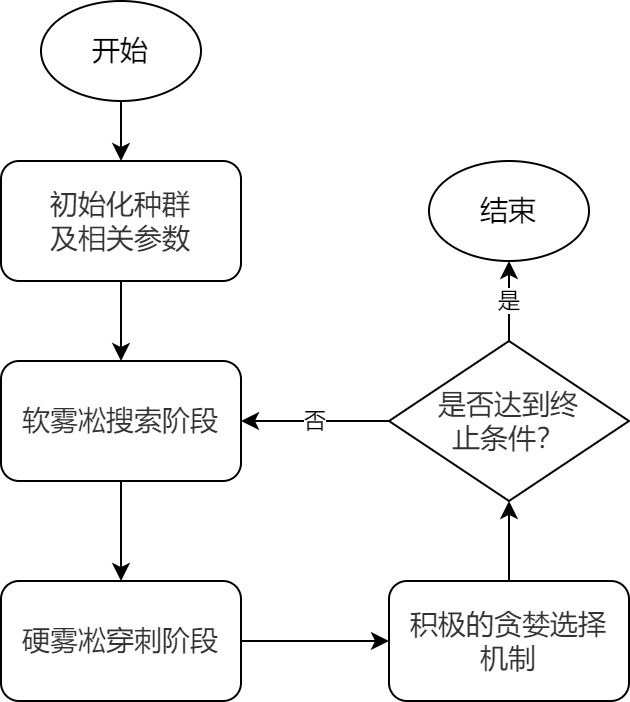
\includegraphics[width=0.7\linewidth]{figures/Flowchart/RIME-Flowcahrt.png} % 调整宽度为适合您文档的值
    \caption{RIME算法流程图}
    \label{fig:RIME-Flowchart}
\end{figure}

\begin{algorithm}[H]
\caption{Pseudo-code of RIME}
\label{alg:RIME}
\textbf{Initialization} the population $R$\;
Get the current optimal agent and its corresponding fitness value\;
\While{$t \le T$}{
    Calculate Coefficient of adherence $E$ by Equation;
    \If{$r_2 < E$}{
        Update agent location using Algorithm \ref{alg:soft-rime-search}\;
    }
    \If{$r_3 \le \text{Normalize fitness of } S_i$}{
        Cross updating between agents using Algorithm \ref{alg:hard-rime-puncture}\;
    }
    \If{$F(R_i^{new}) < F(R_i)$}{
        Update the optimal solution through \textbf{the positive greedy selection}\;
    }
    $t = t + 1$\;
}
\end{algorithm}

\begin{algorithm}[H]
    \caption{Hard-rime puncture}
    \label{alg:hard-rime-puncture}
    \SetAlgoLined
    \KwIn{Initial parameters $t, T, N, \text{Dim}$}
    \While{$t \le T$}{
        \For{$i = 1$ \KwTo $N$}{
            \For{$j = 1$ \KwTo $\text{Dim}$}{
                Calculate the normalized fitness value of the $i$-th agent $F^{\text{norm}}(R_i)$ \;
                \If{$r_4 < F^{\text{norm}}(R_i)$}{
                    Update the value of the corresponding rime particle by \ref{eq:hard-rime location update} \;
                }
            }
        }
        Refresh the best-performing agent and its fitness \;
        $t = t + 1$ \;
    }
\end{algorithm}

\begin{algorithm}[H]
    \caption{Soft-rime search}
    \label{alg:soft-rime-search}
    
    % 模板配置了 linesnumbered，会自动显示行号
    \SetAlgoLined 
    
    % 第1-2行：初始化
    Begin with the population initialization \;
    Select the optimal agent and its corresponding fitness \;
    
    % 第3行：While 循环
    \While{$t \le T$}{
        % 第4行
        Calculate the coefficient of adherence $E$ by Equation 6 \;
        
        % 第5行：For 循环 (i)
        \For{$i = 1$ \KwTo $N$ agents}{
            % 第6行：For 循环 (j)
            \For{$j = 1$ \KwTo $\text{Dim}$}{
                % 第7行：If 判断
                \If{$x < E$}{
                    % 第8行
                    Update the value of the corresponding rime particle by \ref{eq:soft-position-update};
                }
            }
        }
        
        % 第12-13行
        Refresh the best-performing agent and its fitness \;
        $t = t + 1$ \;
    }
\end{algorithm}

\subsection{种群初始化}
种群由 $n$ 个代理 ${S}_{i}$ 组成，每个代理包含 $d$ 个雾凇粒子 ${x}_{ij}$ ，如\ref{eq:rime-population1}所定义。因此，种群 $R$ 可以由粒子矩阵完全表征，如\ref{eq:rime-population2}所示。
\begin{equation}
R = \begin{bmatrix} S_1 \\ S_2 \\ \vdots \\ S_i \end{bmatrix}; S_i = \begin{bmatrix} x_{i1} & x_{i2} & \cdots & x_{ij} \end{bmatrix}
\label{eq:rime-population1}
\end{equation}
\begin{equation}
R = \begin{bmatrix} x_{11} & x_{12} & \cdots & x_{1j} \\ x_{21} & x_{22} & \cdots & x_{2j} \\ \vdots & \vdots & \ddots & \vdots \\ x_{i1} & x_{i2} & \cdots & x_{ij} \end{bmatrix}
\label{eq:rime-population2}
\end{equation}

\subsection{软雾凇搜索}
在有风的环境中，软雾凇的生长具有很强的随机性，使得雾凇粒子能够自由覆盖附着物体的大部分表面，同时在一致的方向上缓慢生长。在软雾凇阶段，雾凇粒子的位置由\ref{eq:soft-position-update}确定。
\begin{equation}
R_{ij}^{new} = R_{best,j} + r_1 \cdot \cos{\theta} \cdot \beta \cdot \left( h \cdot (Ub_{ij} - Lb_{ij}) + Lb_{ij} \right), \, r_2 < E
\label{eq:soft-position-update}
\end{equation}
这里，${R}_{ij}^{\text{ new }}$ 是第 $i$ 个雾凇代理中第 $j$ 个粒子的更新位置，${R}_{\text{ best, }j}$ 表示种群 $R$ 中最佳雾凇代理的第 $j$ 个粒子。方向参数 ${r}_{1}$（$\left( {-1,1}\right)$ 中的随机值）和 $\cos \theta$（\ref{eq:theta}）共同引导粒子运动，并在迭代过程中自适应调整。环境因子 $\beta$（\ref{eq:beta}）通过模拟外部影响确保算法收敛，而粘附系数 $h \in  \left( {0,1}\right)$ 调节粒子间的距离。
\begin{equation}
\theta = \pi \cdot \frac{t}{10 \cdot T}
\label{eq:theta}
\end{equation}
其中 $t$ 表示当前迭代次数，$T$ 是允许的最大迭代次数。
\begin{equation}
\beta = 1 - \left[\frac{w \cdot t}{T}\right] / w
\label{eq:beta}
\end{equation}
其中 $\beta$ 遵循阶梯函数模型，$\left\lbrack  \cdot \right\rbrack$ 表示取整。参数 $w = 5$ 控制阶梯分段的数量。控制个体凝聚概率的附着系数 $E$ 随迭代次数增加（公式 6）。

其中 ${r}_{2} \in  \left( {0,1}\right)$ 是一个均匀分布的随机变量，它与 $E,{242}$ 共同控制粒子凝聚（位置更新）。完整的软雾搜索方法详见算法 2。
\begin{equation}
    E = \sqrt{(\frac {t}{T})}
\label{eq:E}
\end{equation}

\begin{figure}[htbp]
    \centering
    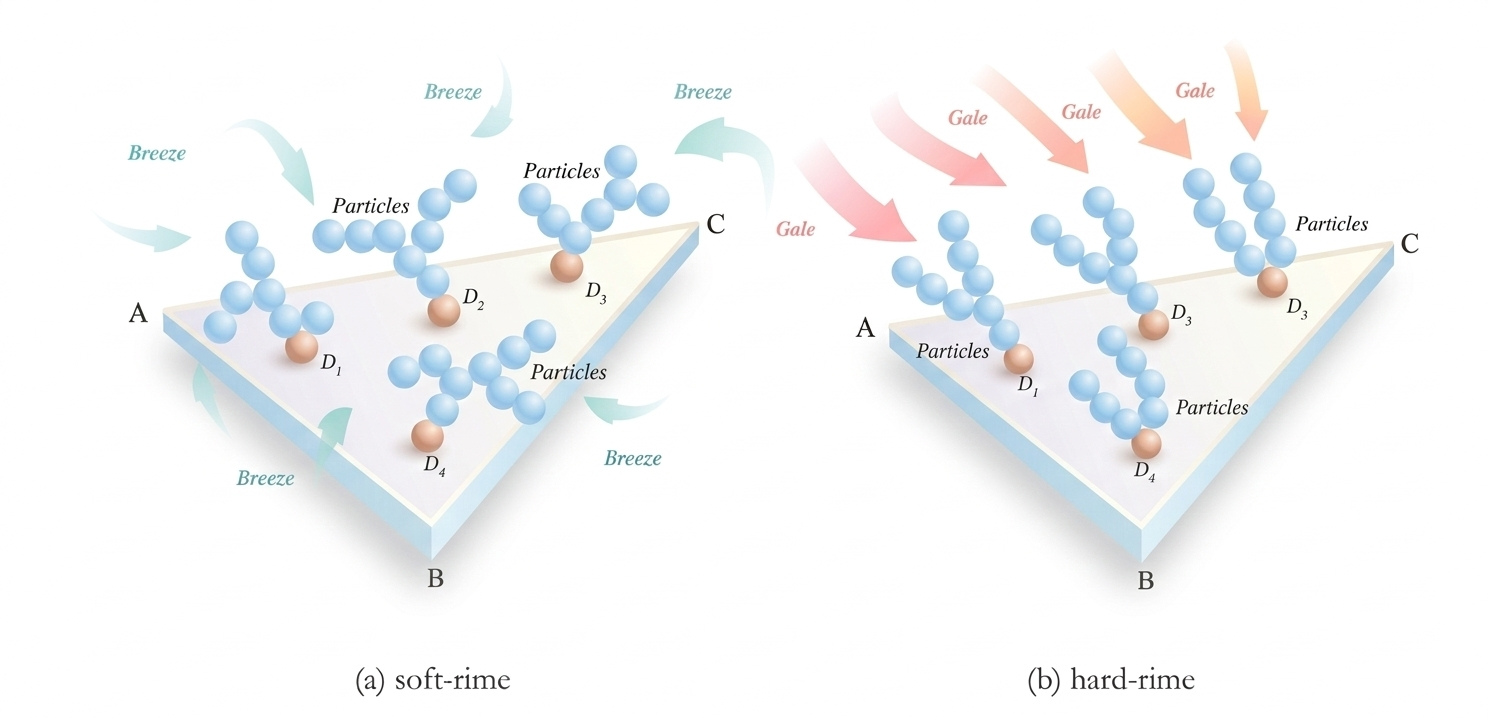
\includegraphics[width=1\linewidth]{figures/RIME/RIMEsoftandhard.png} % 调整宽度为适合您文档的值
    \bicaption{雾凇算法软雾凇搜索和硬雾凇穿刺示意图}{Soft-rime search and hard-rime puncture of RIME}
    \label{fig:RIME-soft-hard}
\end{figure}
\subsection{硬雾凇穿刺}
在大风条件下，硬雾凇生长比软雾凇呈现出更简单、更规则的模式，具有三个关键特征：(1) 强风使外部影响最小化，导致连贯的单向生长。(2) 均匀的生长方向促进粒子重叠。(3) 与软雾凇一样，硬雾凇粒子在生长过程中会膨胀，增加穿刺概率。RIME 算法吸收了这种穿刺机制，增强了收敛性和跳出局部最优的能力。具体实现见\ref{alg:hard-rime-puncture}，粒子替换公式见\ref{eq:hard-rime location update}。

\begin{equation}
R_{ij}^{new} = R_{best,j}, \quad r_3 < F_{normr}(S_i)
\label{eq:hard-rime location update}
\end{equation}

其中 ${R}_{ij}^{\text{ new }}$ 表示更新后粒子的位置，而 ${R}_{\text{ best },j}$ 表示雾凇种群 $R$ 中最优粒子的第 $j$ 个分量。第 $i$ 个智能体的选择概率由其归一化适应度值 ${F}^{\text{ normr }}\left( {S}_{i}\right)$ 给出，并且 ${r}_{3}$ 是在 $\left\lbrack  {-1,1}\right\rbrack$ 内均匀分布的随机变量。

\subsection{正贪婪选择机制}
元启发式优化算法具有一种贪婪选择机制，在每次更新后都会替换并记录最佳适应度值和最佳个体。其典型思路是将个体的更新适应度值与全局最优解进行比较；如果更新后的值优于当前的全局最优解，则替换最优适应度值，并将该个体记录为最优解。这种操作的优点在于简单且快速，但它对种群的探索（exploration）和开发（exploitation）并无实质帮助，仅仅起到记录的作用。

在RIME算法中，提出了一种侵略性贪婪选择机制参与种群更新，以提高全局探索效率。具体思路是将更新后个体的适应度值与该个体更新前的适应度值进行比较：如果更新后的适应度值优于更新前的值，则发生替换，同时这两个个体的解也会被替换。一方面，这种机制通过活跃的个体替换，使种群能够持续保有优秀的个体，从而提高全局解的质量。另一方面，由于种群中个体的具体位置在每次迭代中都会发生显著变化，不可避免地会出现一些比更新前更差的个体，这会对下一次迭代产生负面影响。因此，通过这种操作可以确保种群在每次迭代中都朝着更优的方向进化。

\section{哈里斯鹰算法}
\subsection{算法概述}
哈里斯鹰优化算法 (Harris Hawks Optimization, HHO) 是 Heidari 等人提出的一种新的群智能优化方法, 它的理论依据来自于自然界中哈里斯鹰群体捕猎行为的复杂过程。实际捕猎中, 它会表现出侦察、围捕、追踪、 攻击等各种层次的合作模式，依靠不断改变的捕食行为一步步逼近目标。HHO 把这一自然现象用数学建模的方式表达出来, 在鹰群追逐猎物的时候, 用互动博弈的方式来引导种群个体在搜索空间里找到最优解并达到精准搜寻的目的。

\begin{figure}[htbp]
    \centering
    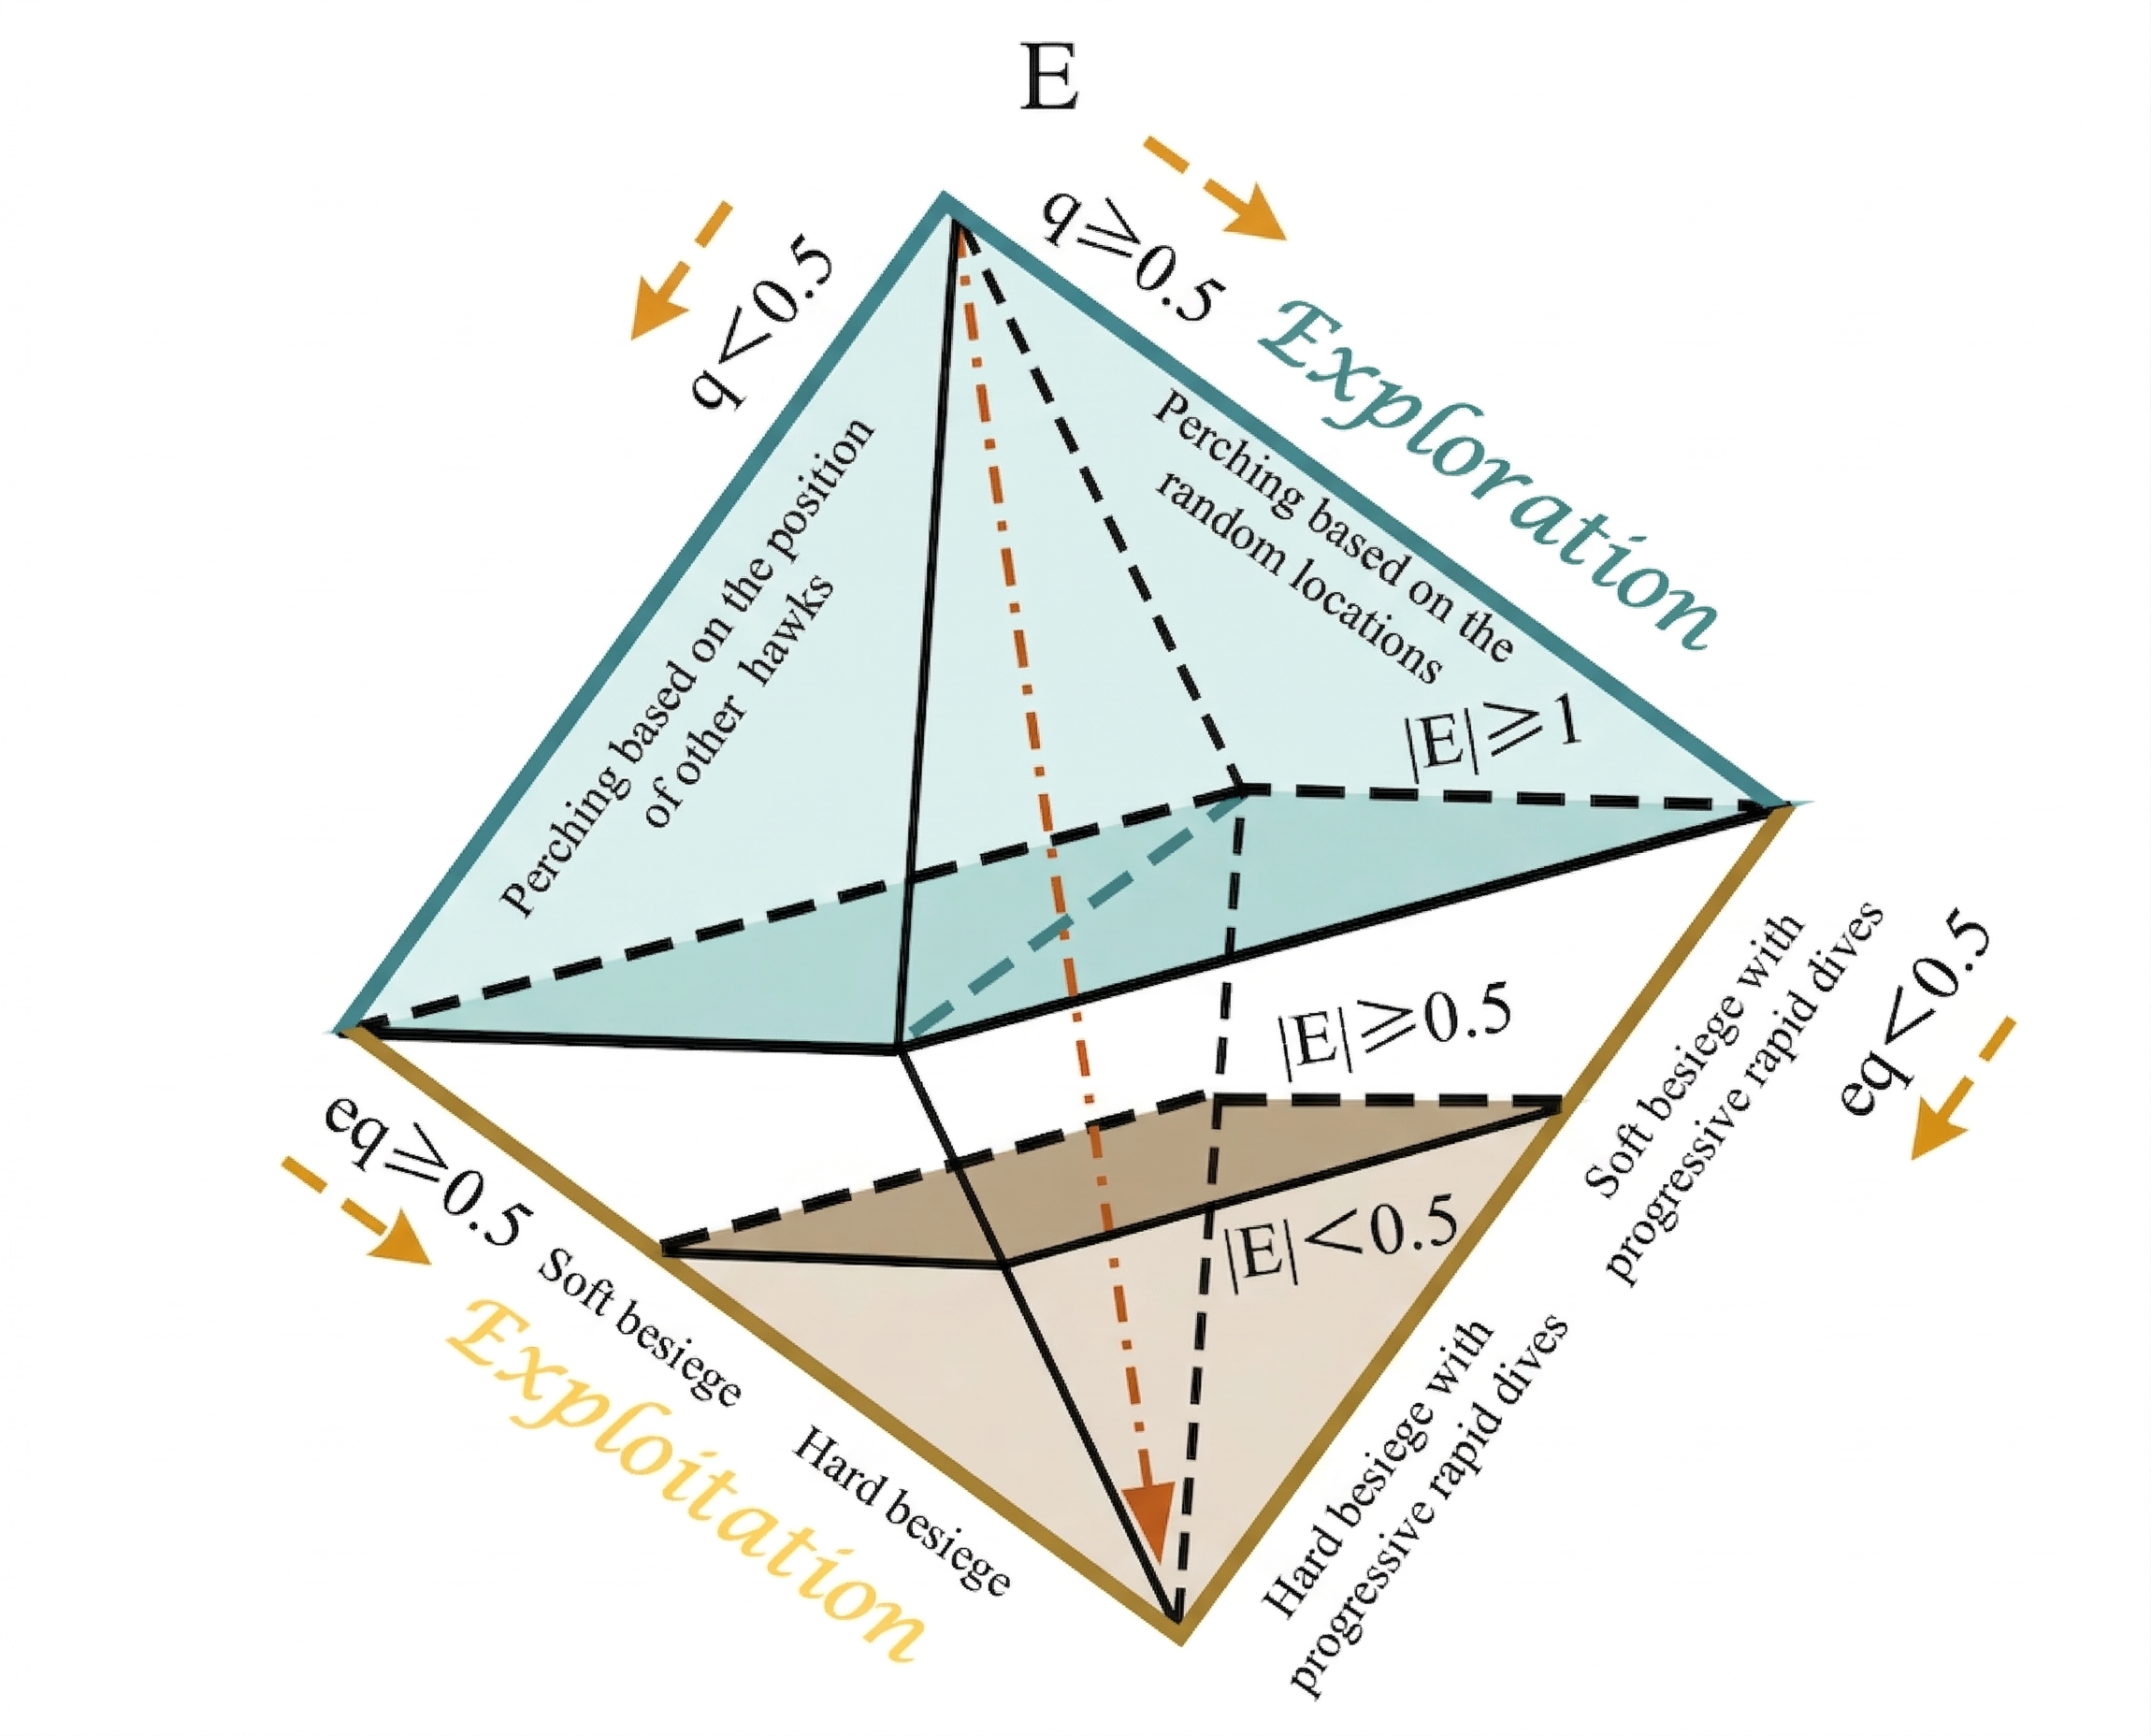
\includegraphics[width=0.8\linewidth]{figures/HHO/all_stage.png} % 调整宽度为适合您文档的值
    \bicaption{HHO各阶段示意图}{All stages of HHO}
    \label{fig:HHO-Stages}
\end{figure}

\subsection{勘探阶段}
在 HHO 中，哈里斯鹰在搜索空间内随机寻找猎物。哈里斯鹰的位置更新取决于猎物的位置和其它鹰的位置。根据随机概率 $q$，算法采用以下两种等概率策略更新鹰的位置：
\begin{equation}
X(t+1) = \begin{cases} X_{rand}(t) - r_1 |X_{rand}(t) - 2r_2 X(t)|, & q \geq 0.5 \\ (X_{rabbit}(t) - X_m(t)) - r_3 (LB + r_4(UB - LB)), & q < 0.5 \end{cases}
\end{equation}
其中，$X(t+1)$ 为第 $t+1$ 次迭代时鹰的位置，$X_{rabbit}(t)$ 为当前猎物（最优解）的位置，$X_{rand}(t)$ 是当前种群中随机选择的鹰的位置，$X_m(t)$ 是当前鹰群的平均位置。$r_1, r_2, r_3, r_4$ 和 $q$ 是 $(0, 1)$ 范围内的随机数。$LB$ 和 $UB$ 分别表示搜索空间的上下界。
\begin{figure}[htbp]
    \centering
    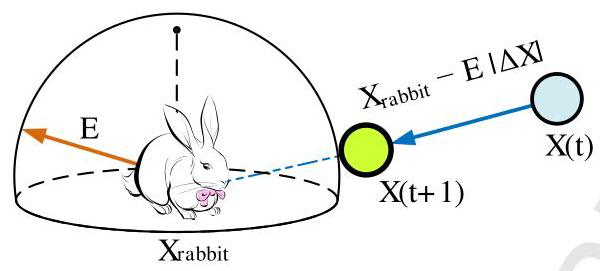
\includegraphics[width=0.8\linewidth]{figures/HHO/bo_d6lgi4f7aajc739e64c0_7_529_286_600_271_0.jpg} % 调整宽度为适合您文档的值
    \bicaption{在硬围攻情况下的矢量示意图}{Example of overall vectors in the case of hard besiege}
    \label{fig:HOO-1}
\end{figure}

\subsection{从勘探到开发的过渡}
HHO 算法通过猎物的逃逸能量 ($E$) 实现从全局勘探到局部开发的动态转换。随着迭代次数的增加，猎物的能量逐渐消耗。逃逸能量的数学模型定义为：
\begin{equation}
E = 2E_0 \left( 1 - \frac{t}{T} \right)
\end{equation}
其中，$E_0$ 是介于 $(-1, 1)$ 之间的初始能量因子。当 $|E| \geq 1$ 时，算法执行勘探阶段，哈里斯鹰在不同区域搜索猎物；当 $|E| < 1$ 时，算法进入局部开发阶段，哈里斯鹰开始包围并攻击猎物。



\subsection{开发阶段}
根据猎物的逃逸行为和鹰的包围策略，开发阶段分为以下四种模式：
\begin{itemize}
\item \textbf{软包围 (Soft Besiege):} 当 $r \geq 0.5$ 且 $|E| \geq 0.5$ 时。此时猎物能量较充沛，试图通过跳跃逃脱，鹰采用缓慢包围策略，消耗猎物能量。
\item \textbf{硬围攻 (Hard Besiege):} 当 $r \geq 0.5$ 且 $|E| < 0.5$ 时。猎物极度疲劳，能量很低，鹰直接进行猛烈突袭。
\item \textbf{渐进式快速俯冲软包围:} 当 $r < 0.5$ 且 $|E| \geq 0.5$ 时。此时猎物还有一定能量，鹰采用更智能的包围策略。引入莱维飞行 (Lévy flight, $LF$) 模拟猎物的不规则逃扑路径：
   \begin{equation}
   Y = X_{rabbit}(t) - E |J X_{rabbit}(t) - X(t)|
   \end{equation}
   \begin{equation}
   Z = Y + S \times LF(D)
   \end{equation}
   其中 $J = 2(1-r_5)$ 表示猎物的跳跃强度。若 $F(Y) < F(X(t))$，则更新位置为 $Y$；否则若 $F(Z) < F(X(t))$，则更新位置为 $Z$。
\item \textbf{渐进式快速俯冲硬围攻:} 当 $r < 0.5$ 且 $|E| < 0.5$ 时。在猎物能量极低时，鹰群通过减小与猎物平均位置的距离来实施攻击，同样结合莱维飞行策略来更新位置。
\end{itemize}


\subsection{HHO 算法伪代码}
HHO 算法伪代码如 Algorithm\ref{alg:HHO} 所示。

\begin{algorithm}[H]
\caption{Harris Hawks Optimization (HHO)}
\label{alg:HHO}
\KwIn{Population size $N$, Max iterations $T$}
\KwOut{The best location of rabbit ($X_{rabbit}$)}
Initialize the random population $X_i (i = 1, 2, ..., N)$\;
\While{$t < T$}{
    Calculate the fitness of each hawk\;
    Set $X_{rabbit}$ as the best location\;
    \For{each hawk ($X_i$)}{
        Update the initial energy $E_0$ and jump strength $J$\;
        Update the escape energy $E$ using Eq. (207)\;
        \If{$|E| \geq 1$}{
            Update location using Exploration Phase (Eq. 200)\;
        }
        \ElseIf{$|E| < 1$}{
            \If{$r \geq 0.5$ and $|E| \geq 0.5$}{
                Soft Besiege\;
            }
            \ElseIf{$r \geq 0.5$ and $|E| < 0.5$}{
                Hard Besiege\;
            }
            \ElseIf{$r < 0.5$ and $|E| \geq 0.5$}{
                Soft Besiege with progressive rapid dives\;
            }
            \ElseIf{$r < 0.5$ and $|E| < 0.5$}{
                Hard Besiege with progressive rapid dives\;
            }
        }
    }
    $t = t + 1$\;
}
\Return $X_{rabbit}$\;
\end{algorithm}


\section{本章小结}
本章围绕特征选择方法与相关优化算法展开背景知识介绍，为后续研究奠定理论基础。在特征选择方法部分，首先明确其核心目标是从原始特征集中筛选最优子集，剔除无关与冗余特征并保留高判别力核心特征，且该问题本质为组合优化问题，在医学超高维数据场景下面临搜索空间爆炸的挑战。随后，介绍了两种基础算法：雾凇算法模拟雾凇形成过程，通过种群初始化、软雾凇搜索、硬雾凇穿刺及正向贪婪选择四阶段平衡探索与开发能力；哈里斯鹰算法模拟鹰群捕猎行为，经勘探阶段、动态过渡及四种开发模式实现精准寻优。两类算法为改进特征选择子集生成策略提供了重要基础。

\chapter{多策略融合改进的雾凇算法}

\section{算法介绍}

\subsection{信息熵评估策略}
信息熵评估策略是信息论中用于衡量数据不确定性的基本概念。其实质是通过概率分布量化系统中的不确定性或随机性：熵值越高，系统的不确定性越大；反之，熵值越低，系统的确定性越强。在优化问题中，信息熵可动态评估种群多样性，从而在优化过程中实现探索与利用之间的自适应平衡。该策略如\Ref{alg:entropy} 所示。
\begin{algorithm}[htbp]
    \caption{Information Entropy Evaluation Strategy}
    \label{alg:entropy}
    \SetAlgoLined
    \KwIn{Population $X = \{x_1, x_2, \dots, x_n\}$ (population size $n$, dimension $m$)}
    \KwOut{Entropy-optimized population $X^{\text{IE}} = \{x_1^{\text{IE}}, x_2^{\text{IE}}, \dots, x_n^{\text{IE}}\}$}
    
    Initialize weight vector $\boldsymbol{w} \leftarrow [0]^m$ \;
    \For{dimension $j = 1$ \KwTo $m$}{
        Compute sum of the $j$-th dimension: $sum_j = \sum_{i=1}^n x_{ij}$ \;
        \If{$sum_j = 0$}{
            \tcp*{Avoid division by zero}
            $p_{ij} \leftarrow 0, \forall i \in [1, n]$ \;
        }
        \Else{
            Compute normalized probability: $p_{ij} = x_{ij} / sum_j, \forall i \in [1, n]$ \;
        }
        Compute entropy $E_j$ by Equation 10 \;
    }
    \For{dimension $j = 1$ \KwTo $m$}{
        Compute the weight $w_j$ by Equation 11 \;
    }
    \For{individual $i = 1$ \KwTo $n$}{
        Update position $X^{\text{IE}}$ through Equation 12 \;
    }
    \Return $X^{\text{IE}}$ \;
\end{algorithm}
\subsubsection{信息熵的数学定义}
设离散随机变量 $\mathcal{X}$ 的概率质量函数为 $P\left( {\mathcal{X} = {x}_{k}}\right)  = 2 \; {p}_{k}$，其中 $k = 1,2,\ldots ,K$。$\mathcal{X}$ 的信息熵 $H\left( \mathcal{X}\right)$ 定义为：
\begin{equation}
    H(\mathcal{X}) = -\sum_{k=1}^K p_k \log_2 p_k
\label{eq:information entropy define}    
\end{equation}
其中 log 表示以 2 为底的对数（熵的单位为比特）或以 e 为底的自然对数（熵的单位为奈特）。
\subsubsection{评估流程}
本文设计了一种名为信息熵评估策略的信息熵驱动动态权重分配策略。该策略可以有效提高启发式算法的收敛效率，其具体步骤如下：

步骤 1：位置概率归一化：对种群中第 $j$ 维特征的位置值进行归一化，并计算该维度上第 $i$ 个个体的变异概率：
\begin{equation}
    p_{ij} = \frac{x_{ij}}{\sum_{i=1}^n x_{ij}}
\label{eq:mutation probability p}
\end{equation}
其中 ${x}_{ij}$ 表示第 $i$ 个个体在第 $j$ 维的位置，$n$ 是种群大小。

步骤 2：维度熵计算：基于归一化结果，计算第 $j$ 维的信息熵 ${E}_{j}$：
\begin{equation}
E_j = \begin{cases} 
0 & \text{if } \sum_{i=1}^n x_{ij} = 0, \\
-\frac{1}{\ln n} \sum_{i=1}^n p_{ij} \ln p_{ij} & \text{otherwise.}
\end{cases}
\label{eq:information entropy E}
\end{equation}
其中 $\ln n$ 是确保 ${E}_{j} \in  \left\lbrack  {0,1}\right\rbrack$ 的归一化因子。

步骤 3：特征权重分配：基于第 $j$ 维的熵 ${E}_{j}$ 计算其权重 ${w}_{j}$，其中熵越低（确定性越高）对应越大的权重。

\begin{equation}
    w_j = \frac{1 - E_j}{\sum_{k=1}^m (1 - E_k)}
\label{eq:feature weight}
\end{equation}
其中 $m$ 表示特征维度的总数。

步骤 4：更新智能体位置：使用权重 ${w}_{j}$ 调整个体位置，生成新的熵优化位置 ${x}_{i}^{\mathrm{{IE}}}$：
% \begin{equation}
%     x_i^{\text{IE}} = x_i \odot \boldsymbol{w}
% \label{eq:new entropy-optimized positions}
% \end{equation}

其中 $\odot$ 表示逐元素相乘，$\mathbf{w} = {\left\lbrack  {w}_{1},{w}_{2},\ldots ,{w}_{m}\right\rbrack  }^{\top }$ 是权重向量。
\subsection{拉格朗日插值法}
拉格朗日插值法利用预定义的节点构建目标函数的多项式近似。从该插值多项式得到的最优解可作为原函数最优解的近似。随着节点间的间隔减小，多项式的最优解会收敛到原函数的最优解。\\ 拉格朗日插值公式表示为：

\begin{equation}
    P_n(x) = \sum_{j=1}^n y_j \left( \prod_{\substack{i=1 \\ i \neq j}}^{k} \frac{x - x_i}{x_j - x_i} \right)
\label{eq:Lagrange interpolation}
\end{equation}

其中 $\left( {{x}_{i},{y}_{i}}\right)$ 表示第 $i$ 个节点的坐标，$n\mathrm{n}$ 对应所选节点的数量，$j$ 表示一个与 $i$ 不同的索引。当 $n = 1$ 时，得到的表达式是一个常数函数；当 $n = 2$ 时，得到的多项式是一个线性函数，对于解决复杂问题，它与目标函数的相似度不足；当 $n > 4$ 时，得到的多项式至少是一个三次函数，其最优解需要大量的计算成本和导数信息，不适合用于优化。因此，本文选择 $n = 3$，得到一个多项式。
\begin{equation}
    P_3(x) = y_0 \times \frac{(x-x_1)(x-x_2)}{(x_0-x_1)(x_0-x_2)} + y_1 \times \frac{(x-x_0)(x-x_2)}{(x_1-x_0)(x_1-x_2)} + y_2 \times \frac{(x-x_0)(x-x_1)}{(x_2-x_0)(x_2-x_1)}
\label{eq:P3}
\end{equation}
设，
\begin{equation}
    a_0 = \frac{y_0}{(x_0-x_1)(x_0-x_2)}, \quad a_1 = \frac{y_1}{(x_1-x_0)(x_1-x_2)}, \quad a_2 = \frac{y_2}{(x_2-x_0)(x_2-x_1)}
\label{eq:a0-a1-a2}
\end{equation}

${P}_{3}\left( x\right)$ 的最优解可轻松得到为
\begin{equation}
    x^* = \frac{a_0(x_1+x_2) + a_1(x_0+x_2) + a_2(x_0+x_1)}{2(a_0+a_1+a_2)}
\label{eq:X*}
考虑到优化问题的多维性质，我们对上述公式 342 进行了改进，得到以下表达式：
\end{equation}

\begin{equation}
    X_L = \frac{a_0(X_{(r,t)}(t) + Best(t)) + a_1(X_{(r,s)}(t) + Best(t)) + a_2(X_{(r,s)}(t) + X_{(r,t)}(t))}{2(a_0+a_1+a_2)}
\label{eq:XL}
\end{equation}
\begin{equation}
\left\{
\begin{aligned}
a_0 &= \frac{f(X_{r3}(t))}{(X_{r3}(t)-X_{r4}(t))(X_{r3}(t)-\text{Best}(t))} \\
a_1 &= \frac{f(X_{r4}(t))}{(X_{r4}(t)-X_{r3}(t))(X_{r4}(t)-\text{Best}(t))} \\
a_2 &= \frac{f(\text{Best}(t))}{(\text{Best}(t)-X_{r3}(t))(\text{Best}(t)-X_{r4}(t))}
\end{aligned}
\right.
\label{eq:a0-a1-a2-2}
\end{equation}
其中 ${X}_{L}$ 表示通过拉格朗日插值得到的新位置，${X}_{\left( r3\right) }\left( t\right)$ 和 ${X}_{\left( r4\right) }\left( t\right)$ 表示两个随机选择的个体的位置，Best $\left( t\right)$ 表示当前最优个体的位置。该策略的伪代码如算法 \ref{alg:lagrange} 所示。
\begin{algorithm}[htbp]
    \caption{Lagrange Interpolation Method}
    \label{alg:lagrange}
    \SetAlgoLined
    \KwIn{Population $P(t) = \{X_1(t), X_2(t), \dots, X_N(t)\}$; current best individual $Best(t)$}
    \KwOut{New position $X_L$}
    
    Randomly select two distinct individuals $X_{(r3)}(t)$ and $X_{(r4)}(t)$ from $P(t)$ \;
    Compute coefficients $a_0, a_1, a_2$ according to Equation 17 and Equation 20 \;
    Update new position $X_L$ through Equation 19 \;
\end{algorithm}
\subsection{随机重启机制}
传统的重启策略通常在预定的迭代次数后触发，无法及时重启表现不佳的个体。这会干扰表现良好个体的搜索过程，同时让过多表现不佳的解使算法陷入次优解。为克服这一局限，我们提出一种更具随机性的重启策略。当迭代次数超过 ${T}_{\text{ rand }}$ 时，算法重启按适应度值排名靠后的一半个体。这种方法在保留高质量个体的同时确保刷新表现不佳的解，从而保持收敛精度和速度。此外，随机化的迭代阈值显著增强了种群多样性，有效减轻了次优解的负面影响。随机重启策略正式定义如下：
\begin{equation}
    T_{\text{rand}} = T \times \sin\left(\pi \cdot \text{rand}\right) 
\label{eq:rand number T}
\end{equation}
\begin{equation}
    X_i^{\text{inferior}} = \text{lb} \times \text{rand} + (\text{ub} - \text{lb}) \times \text{rand} \times \text{randi}(-1,1)
\label{eq:X-inferior}
\end{equation}
其中 ${T}_{\text{ rand }}$ 表示随机化的迭代阈值，${X}_{i}^{\text{ inferior }}$ 表示第 $i$ 个次优智能体的位置，${lb}$ 和 ${ub}$ 分别表示搜索域的下界和上界。randi $\left( {-1,1}\right)$ 是在 $\left\lbrack  {-1,1}\right\rbrack$ 内均匀分布的随机变量。

\subsection{时间复杂度分析}
IRIME 算法的时间复杂度包括：参数定义 O(1)、种群初始化 $\mathrm{O}\left( {\mathrm{n} \cdot  \mathrm{d}}\right)$、信息熵评估 $\mathrm{O}\left( {\mathrm{T} \cdot  \mathrm{n} \cdot  \mathrm{d}}\right)$、随机重启机制 $\mathrm{O}\left( {\mathrm{T} \cdot  \mathrm{n} \cdot  \mathrm{d}}\right)$、拉格朗日插值 $\mathrm{O}\left( {\mathrm{T} \cdot  \mathrm{n} \cdot  \mathrm{d}}\right)$、评估函数计算 $\mathrm{O}\left( {\mathrm{T} \cdot  \mathrm{n} \cdot  \mathrm{c}}\right)$ 和种群更新 $\mathrm{O}\left( {\mathrm{T} \cdot  \mathrm{n} \cdot  \mathrm{d}}\right)$。总体复杂度为 $\mathrm{O}\left( 1\right) \; + \mathrm{O}\left( {\mathrm{n} \cdot  \mathrm{d}}\right)  + \mathrm{O}\left( {\mathrm{T} \cdot  \mathrm{n} \cdot  \mathrm{c}}\right)  + 3 \cdot  \mathrm{O}\left( {\mathrm{T} \cdot  \mathrm{n} \cdot  \mathrm{d}}\right)$，其中 $\mathrm{n}$ 是种群大小，$\mathrm{d}$ 是问题维度，c 是评估函数计算时间。

\begin{figure}
    \centering
    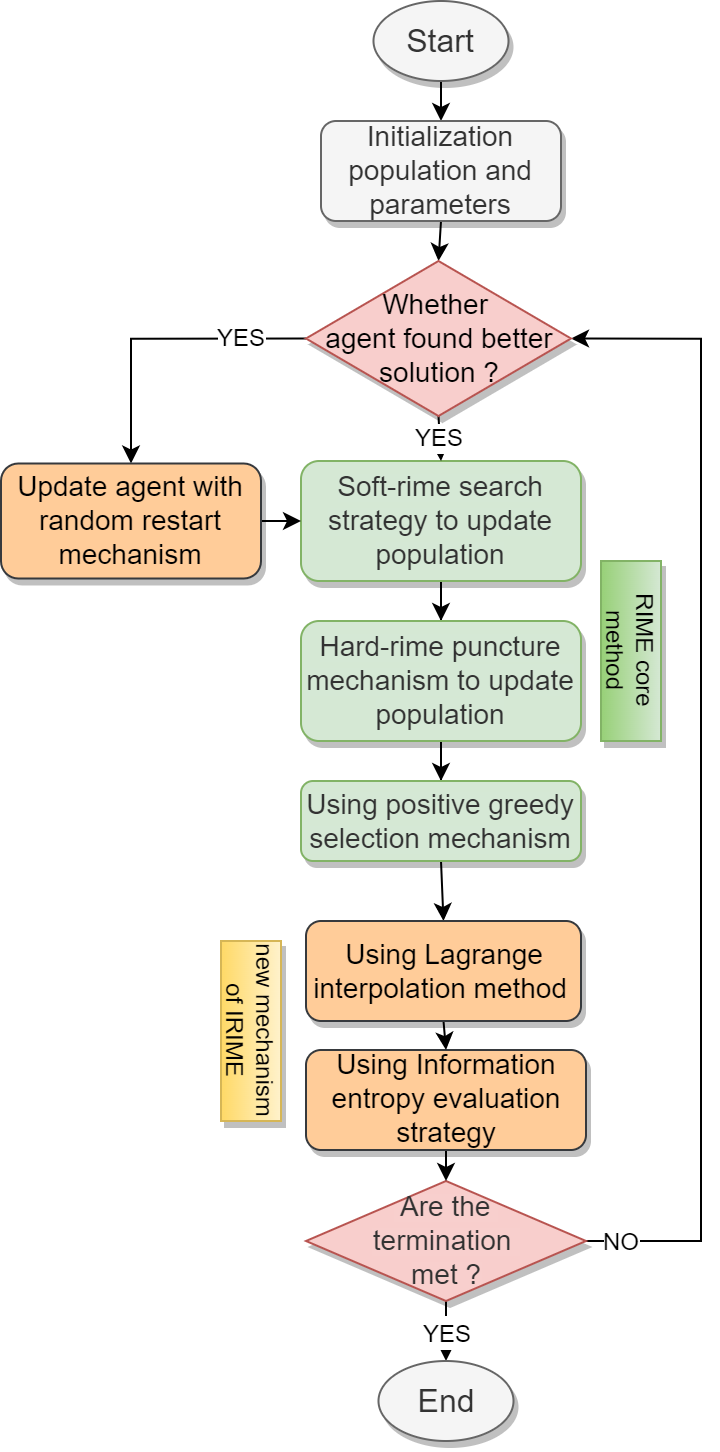
\includegraphics[width=0.6\linewidth]{figures//Flowchart/IRIME2flowchart.png}
    \bicaption{IRIME工作流程图}{Flowchart of IRIME}
    \label{fig:Flowchart-IRIME}
\end{figure}

\begin{algorithm}[htbp]
    \caption{Pseudo-code of IRIME}
    \label{alg:irime}
    \SetAlgoLined
    Initialization the rime population \;
    Get the current optimal agent and optimal fitness \;
    \While{$t \le T$}{
        Using \textbf{the random restart mechanism} for those who cannot find a better solution \;
        Calculate coefficient of adherence $E$ by Equation 6 \;
        \If{$r_2 < E$}{
            Update rime agent location using Algorithm 2 \;
        }
        \If{$r_3 < S_i$}{
            \tcp*{$S_i$: normalized fitness}
            Cross updating between agents using Algorithm 3 \;
        }
        \If{$F(R_i^{\text{new}}) < F(R_i)$}{
            Select the optimal solution and replace suboptimal solution using \textbf{the positive greedy selection} \;
        }
        Run the Algorithm 6 \;
        Run the Algorithm 5 \;
        $t = t + 1$ \;
    }
\end{algorithm}

\newpage

\section{实验设计}\label{sec:exp-settings}
本节介绍所设计了三个实验：CEC 2017 基准函数对比实验、医学数据集下的特征选择应用实验、和消融实验。分别对IRIME的理论性能和应用价值进行验证，并通过消融实验验证所引入策略的合理性与必要性。我们的实验框架采用了严格的评估指标，包括 30 次独立运行的最佳适应度值（Best）、平均性能（Mean）和标准差（Std）。CEC 2017 测试套件的定义和详细信息见表 2。所有实验均在配备英特尔酷睿 i5 - 12600KF 2.50GHz 处理器、16GB 内存、运行 Windows 11（64 位）的工作站上进行，使用 MATLAB R2021a。为保证统计可靠性，每个算法独立运行 30 次，每次运行的终止条件为 10000 次函数评估。为确保公平比较，我们保持一致的实验条件：所有算法的种群规模固定为 30，并严格遵循其最初公布的参数设置。

\subsection{基准函数对比实验}
在本节中，我们通过在 CEC 2017 测试集上进行广泛的实验，将所提出的 IRIME 算法与八个先进的竞争对手进行了评估。所有对比算法的参数配置列于表 1。研究涵盖三个关键分析维度：(1) 通过迭代曲线进行收敛行为分析，(2) 通过箱线图可视化进行解的稳定性评估，(3) 使用弗里德曼检验进行非参数统计验证。所有实验均在严格控制的条件下进行。第 \ref{sec:exp-settings} 节详细介绍了软件和硬件配置。
\begin{table}[ht]
\centering
\footnotesize
\caption{CEC 2017 测试套件函数的详细信息}
\label{tb:CEC2017-functions}
\begin{tabular}{>{\ttfamily}l l l r}
\toprule
\textbf{ID} & \textbf{Function Equation} & \textbf{Class} & \textbf{Optimum} \\
\midrule
F1  & Shifted and Rotated Bent Cigar Function          & Unimodal    & 100   \\
F3  & Shifted and Rotated Zakhov Function              & Unimodal    & 300   \\
F4  & Shifted and Rotated Rosenbrock's Function        & Multimodal  & 400      \\
F5  & Shifted and Rotated Rastrin's Function           & Multimodal  & 500   \\
F6  & Shifted and Rotated Expanded Scaffer's F6 Function & Multimodal  & 600   \\
F7  & Shifted and Rotated Lunacek Bi-Rastrigin Function  & Multimodal  & 700   \\
F8  & Shifted and Rotated Non-Continuous Rastrigin's Function & Multimodal & 800   \\
F9  & Shifted and Rotated Lévy Function                & Multimodal  & 900   \\
F10  & Shifted and Rotated Schwefel's Function          & Multimodal  & 1000  \\
F11 & Hybrid Function 1 (N=3)                          & Hybrid      & 1100  \\
F12 & Hybrid Function 2 (N=3)                          & Hybrid      & 1200  \\
F13 & Hybrid Function 3 (N=3)                          & Hybrid      & 1300  \\
F14 & Hybrid Function 4 (N = 4)                        & Hybrid      & 1400  \\
F15 & Hybrid Function 5 (N=4)                          & Hybrid      & 1500  \\
F16 & Hybrid Function 6 (N=6)                          & Hybrid      & 1600  \\
F17 & Hybrid Function 7 (N = 5)                        & Hybrid      & 1700  \\
F18 & Hybrid Function 8 (N=5)                          & Hybrid      & 1800      \\
F19 & Hybrid Function 9 (N=6)                         & Hybrid      & 1900  \\
F20 & Hybrid Function 10 (N=6)                         & Hybrid      & 2000  \\
F21 & Composition Function 1 (N=3)                     & Composition & 2100  \\
F22 & Composition Function 2 (N=3)                     & Composition & 2200  \\
F23 & Composition Function 3 (N=3)                     & Composition & 2300  \\
F24 & Composition Function 4 (N=3)                     & Composition & 2400  \\
F25 & Composition Function 5 (N=3)                     & Composition & 2500  \\
F26 & Composition Function 6 (N=3)                     & Composition & 2600  \\
F27 & Composition Function 7 (N=3)                     & Composition & 2700  \\
F28 & Composition Function 8 (N=3)                     & Composition & 2800  \\
F29 & Composition Function 9 (N=3)                     & Composition & 2900  \\
F30 & Composition Function 10 (N=3)                     & Composition & 3000  \\
\bottomrule
\end{tabular}
\end{table}

\subsubsection{实验准备}
本实验所选取的算法及算法参数设置如\ref{tb:alg-parameters-1}表所示。本实验所涉及的CEC 2017数据集的相关信息在\ref{tb:CEC2017-functions}表中详细展示。
%算法参数设置表1
\begin{table}[htbp]
\centering
\small
\caption{基准测试中对比算法的参数配置}
\begin{tabular}{ll}
\toprule
\textbf{Algorithms} & \textbf{Other parameters} \\
\midrule
IRIME & $w = 5$ \\
RIME & $w=5$ \\
LSHADE & $p\_best\_rate = 0.11$; $arc\_rate = 2.6$;\\ & $memory\_size = 6$; $NP\_min$ = 4\\
BDA & $w\in [0.5,0.9]$\\
BWO & $W_f \in [0.1,0.5]$\\
RSA & $\alpha = 0.1$; $\beta = 0.005$\\
SCA & $C_1 \in [0,2]$; $C_2 \in [0,2]$;$C_3 \in [0,2]$\\
STOA & $S_a \in [0,2]$; $b = 1$\\
PDO & $rho = 0.005$; $epsPD = 0.1$\\
\bottomrule
\end{tabular}
\label{tb:alg-parameters-1}
\end{table}


\subsubsection{收敛曲线分析}
根据收敛图（图 3 和图 4），在多个函数（如 F1、F10、F13、F15、F19 和 F22）上，IRIME 在收敛速度和最优适应度值方面优于其他八种算法。半对数图揭示了三种不同的收敛模式：（1）初始阶段快速收敛。对于单峰函数（F1、F5），与 RIME 和 LSHADE 相比，IRIME 在前 20\% 的函数评估次数（FEs）内（例如，F1 在 3000 次 FEs 时）实现了更低的适应度值，显示出卓越的初始收敛速度。（2）中后期持续优化。在多峰函数（F6、F15）中，IRIME 保持单调改进，而竞争对手则出现振荡或过早停滞。在 5000 - 10000 次 FEs 期间，其平均梯度比 PDO 更陡峭。（3）在解的质量和稳定性方面，复合函数（F22、F30）展示了 IRIME 卓越的持续优化能力，在实现更好的最终解方面始终优于竞争算法。此外，对比实验（表 3 和表 4）的详细数据表明，IRIME 在三个关键指标：最佳适应度（Best）、平均适应度（Mean）和标准差（Std）上始终优于 RIME、LSHADE、BDA、BWO、RSA、SCA、STOA 和 PDO。例如，在 30 维的 F1 函数上，IRIME 实现了 ${3.95} \times  {10}^{2}$ 的最佳适应度值，远低于其他算法获得的值。同样，对于 50 维的 F4 函数，IRIME 达到了 ${5.14} \times  {10}^{2}$ 的最佳值，再次证明了其卓越的优化能力。值得注意的是，IRIME 在大多数基准函数上保持始终较低的平均值，这不仅表明其平均性能更好，而且解的稳定性更高。其较小的标准差进一步支持了这一结论，表明结果的离散度显著降低，从而提高了算法的可靠性。
% 30维曲线图
\begin{figure}[htbp]
    \centering
    % 第一行子图 (F1, F2, F3)
    \begin{subfigure}[b]{0.32\textwidth}
        \caption*{}
        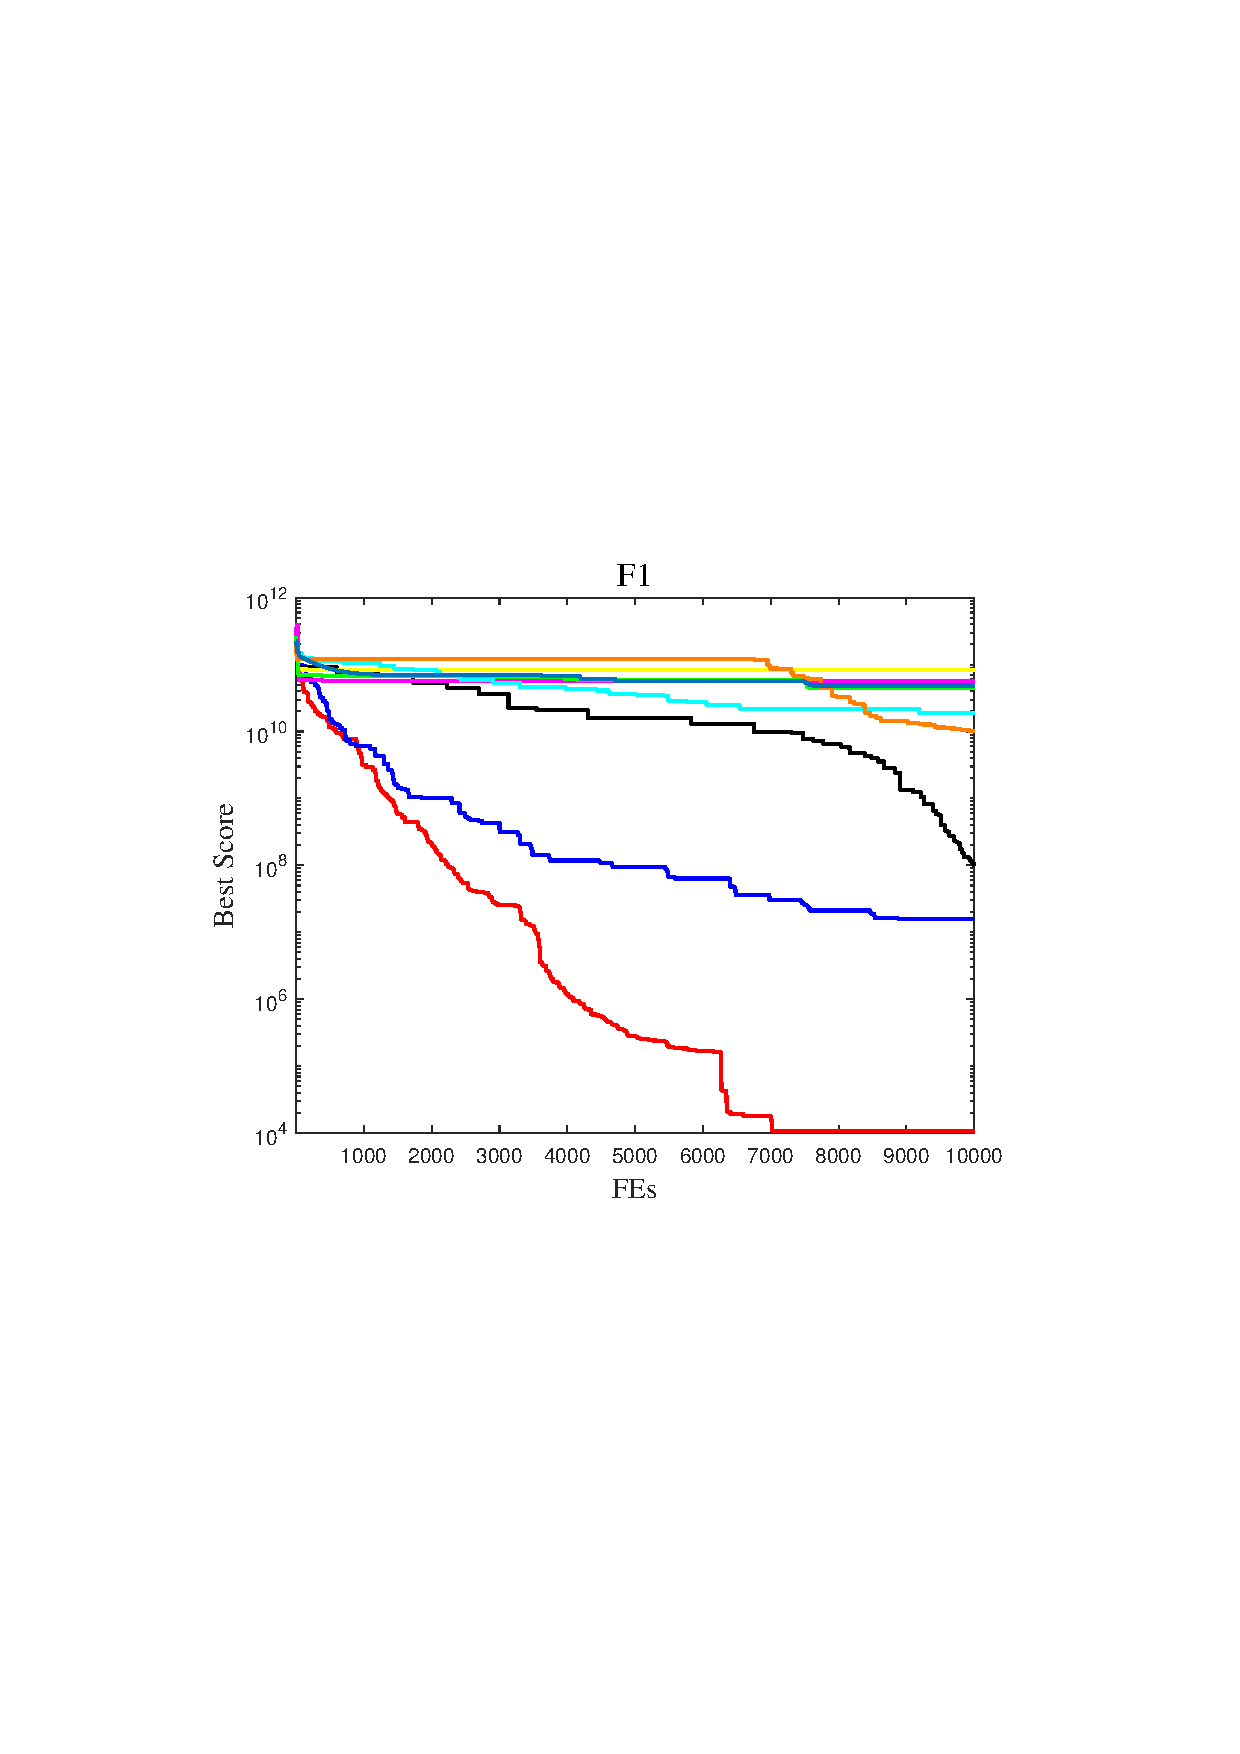
\includegraphics[width=\textwidth]{figures/Convergence/dim30/1.pdf}
    \end{subfigure}
    \hfill
    \begin{subfigure}[b]{0.32\textwidth}
        \caption*{}
        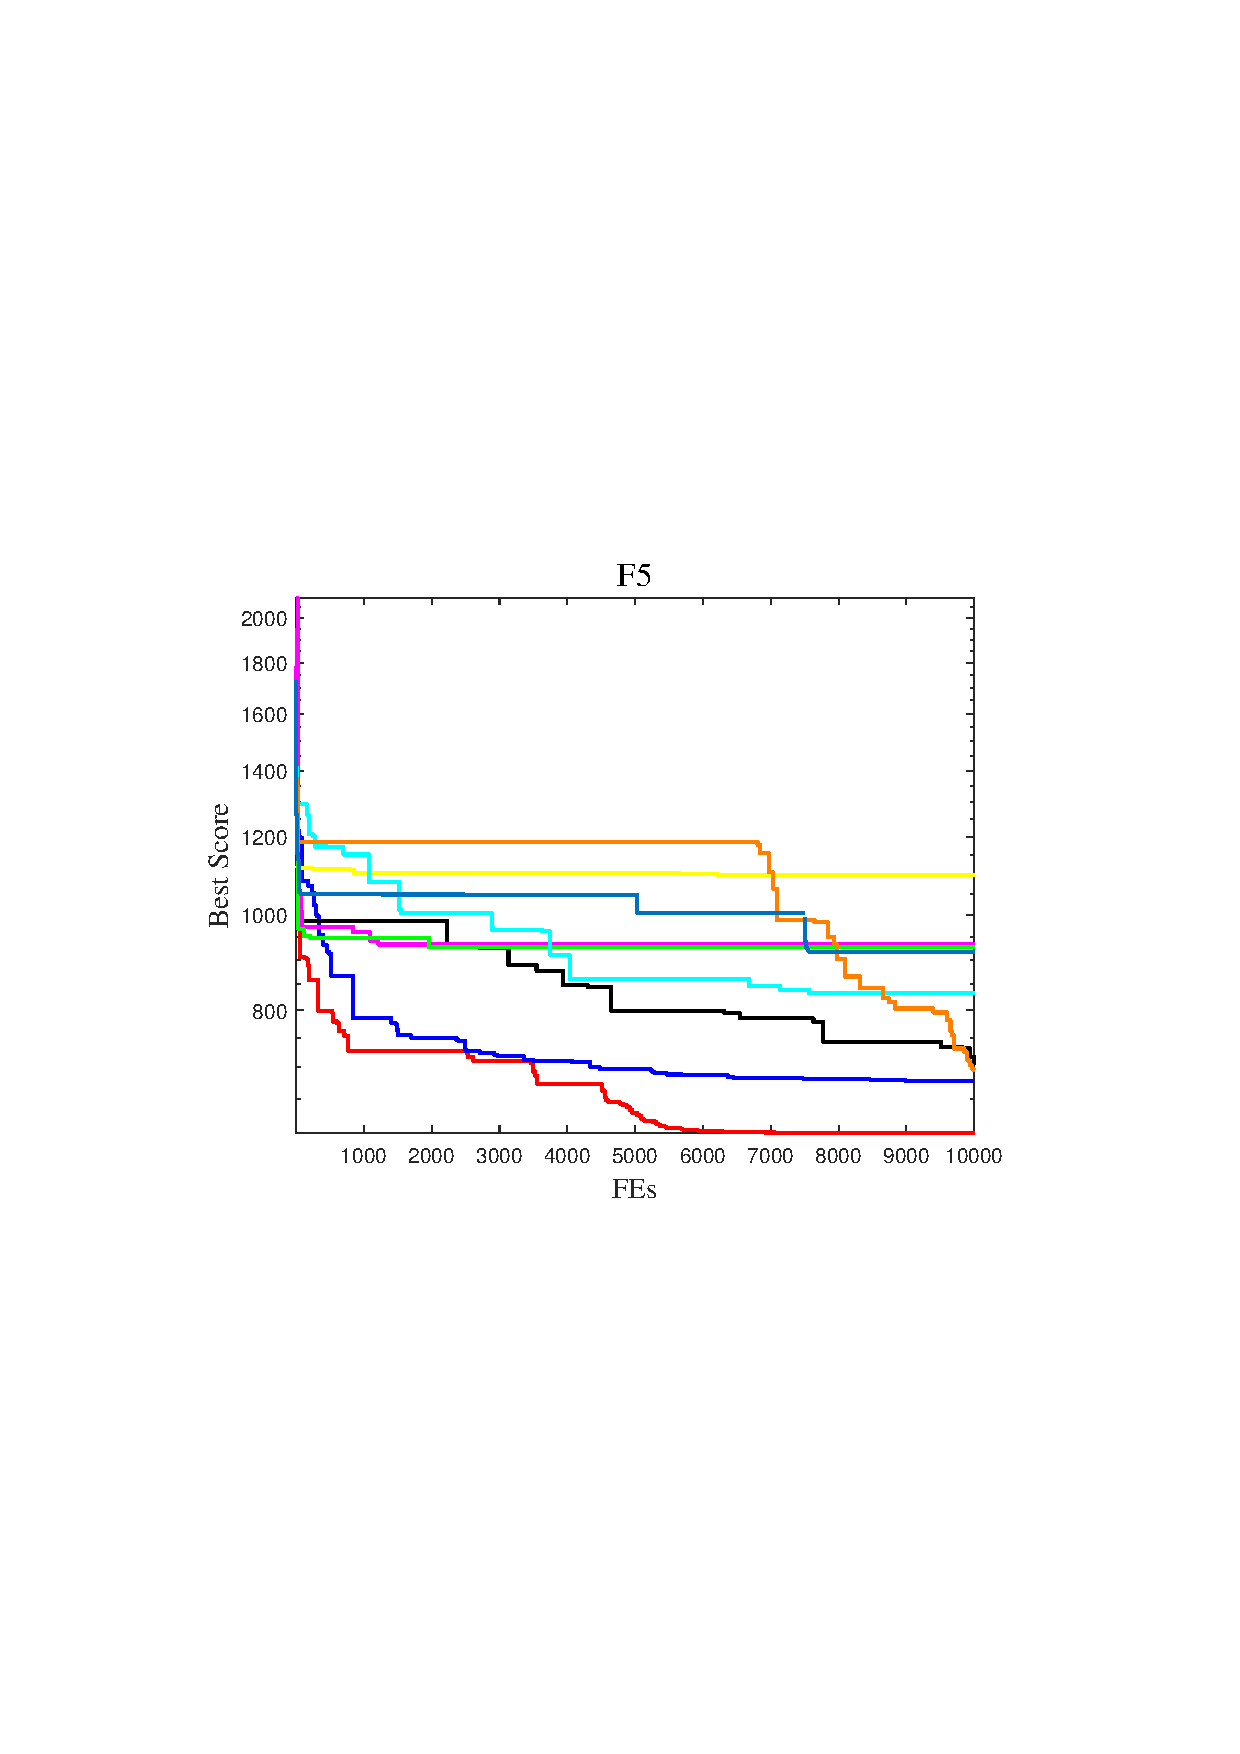
\includegraphics[width=\textwidth]{figures/Convergence/dim30/5.pdf}
    \end{subfigure}
    \hfill
    \begin{subfigure}[b]{0.32\textwidth}
        \caption*{}
        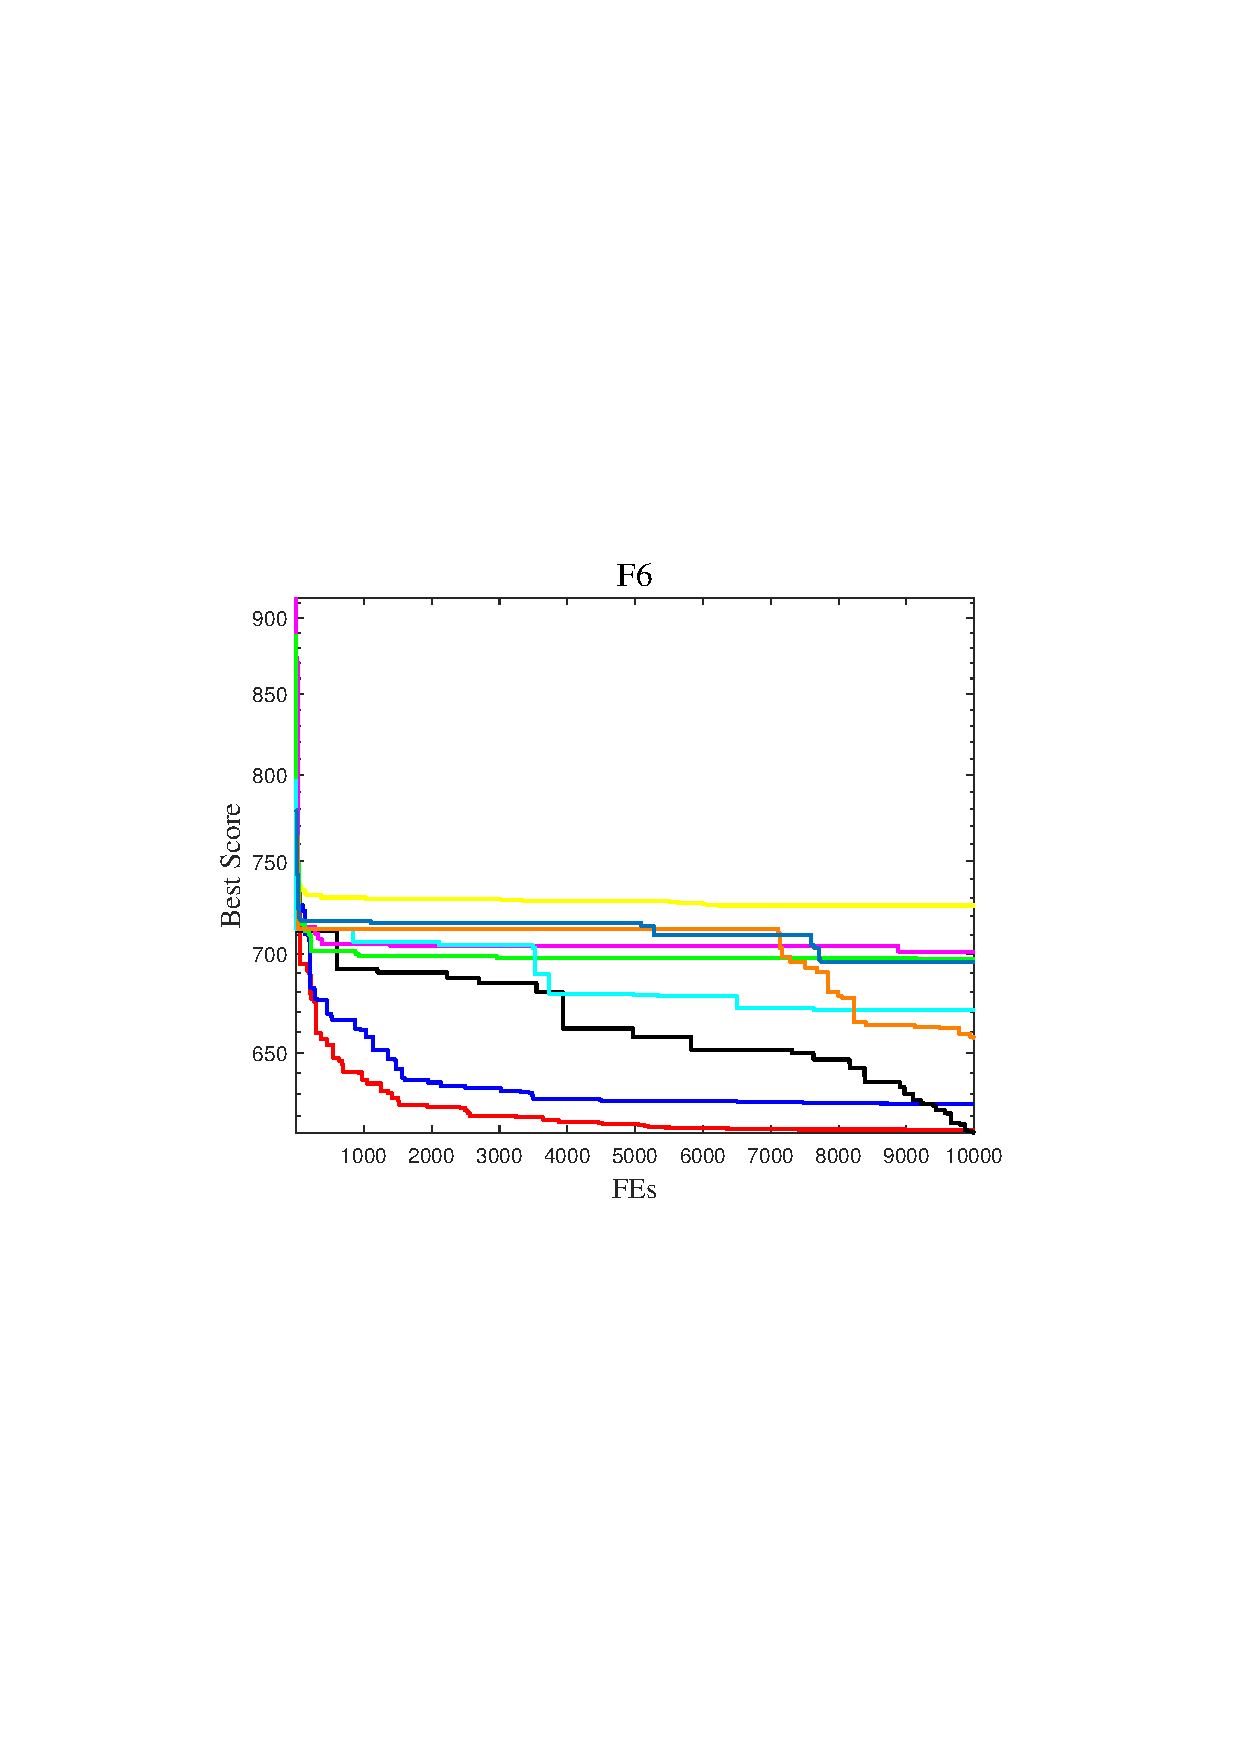
\includegraphics[width=\textwidth]{figures/Convergence/dim30/6.pdf}
    \end{subfigure}
    % 第二行子图 (F6, F11, F16)
    \begin{subfigure}[b]{0.32\textwidth}
        \caption*{}
        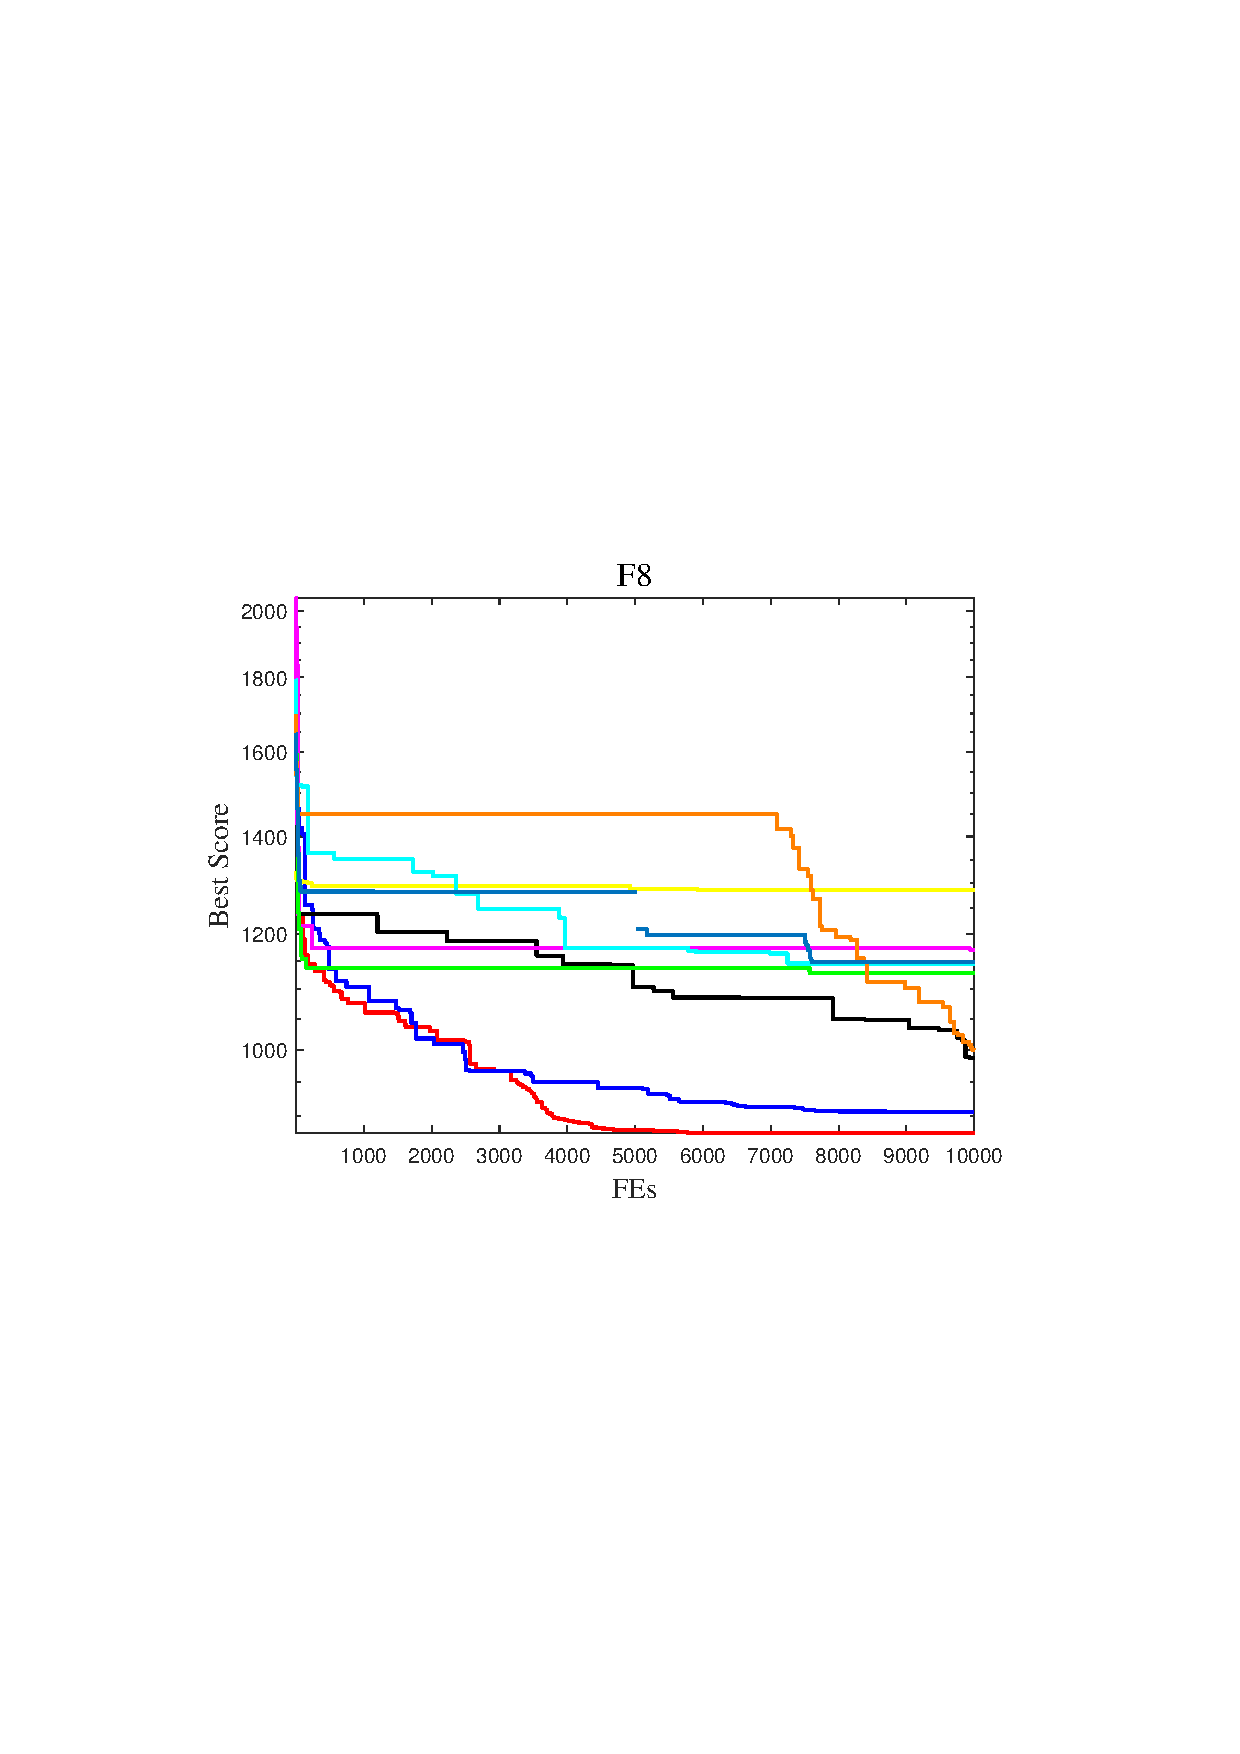
\includegraphics[width=\textwidth]{figures/Convergence/dim30/8.pdf}
    \end{subfigure}
    \hfill
    \begin{subfigure}[b]{0.32\textwidth}
        \caption*{}
        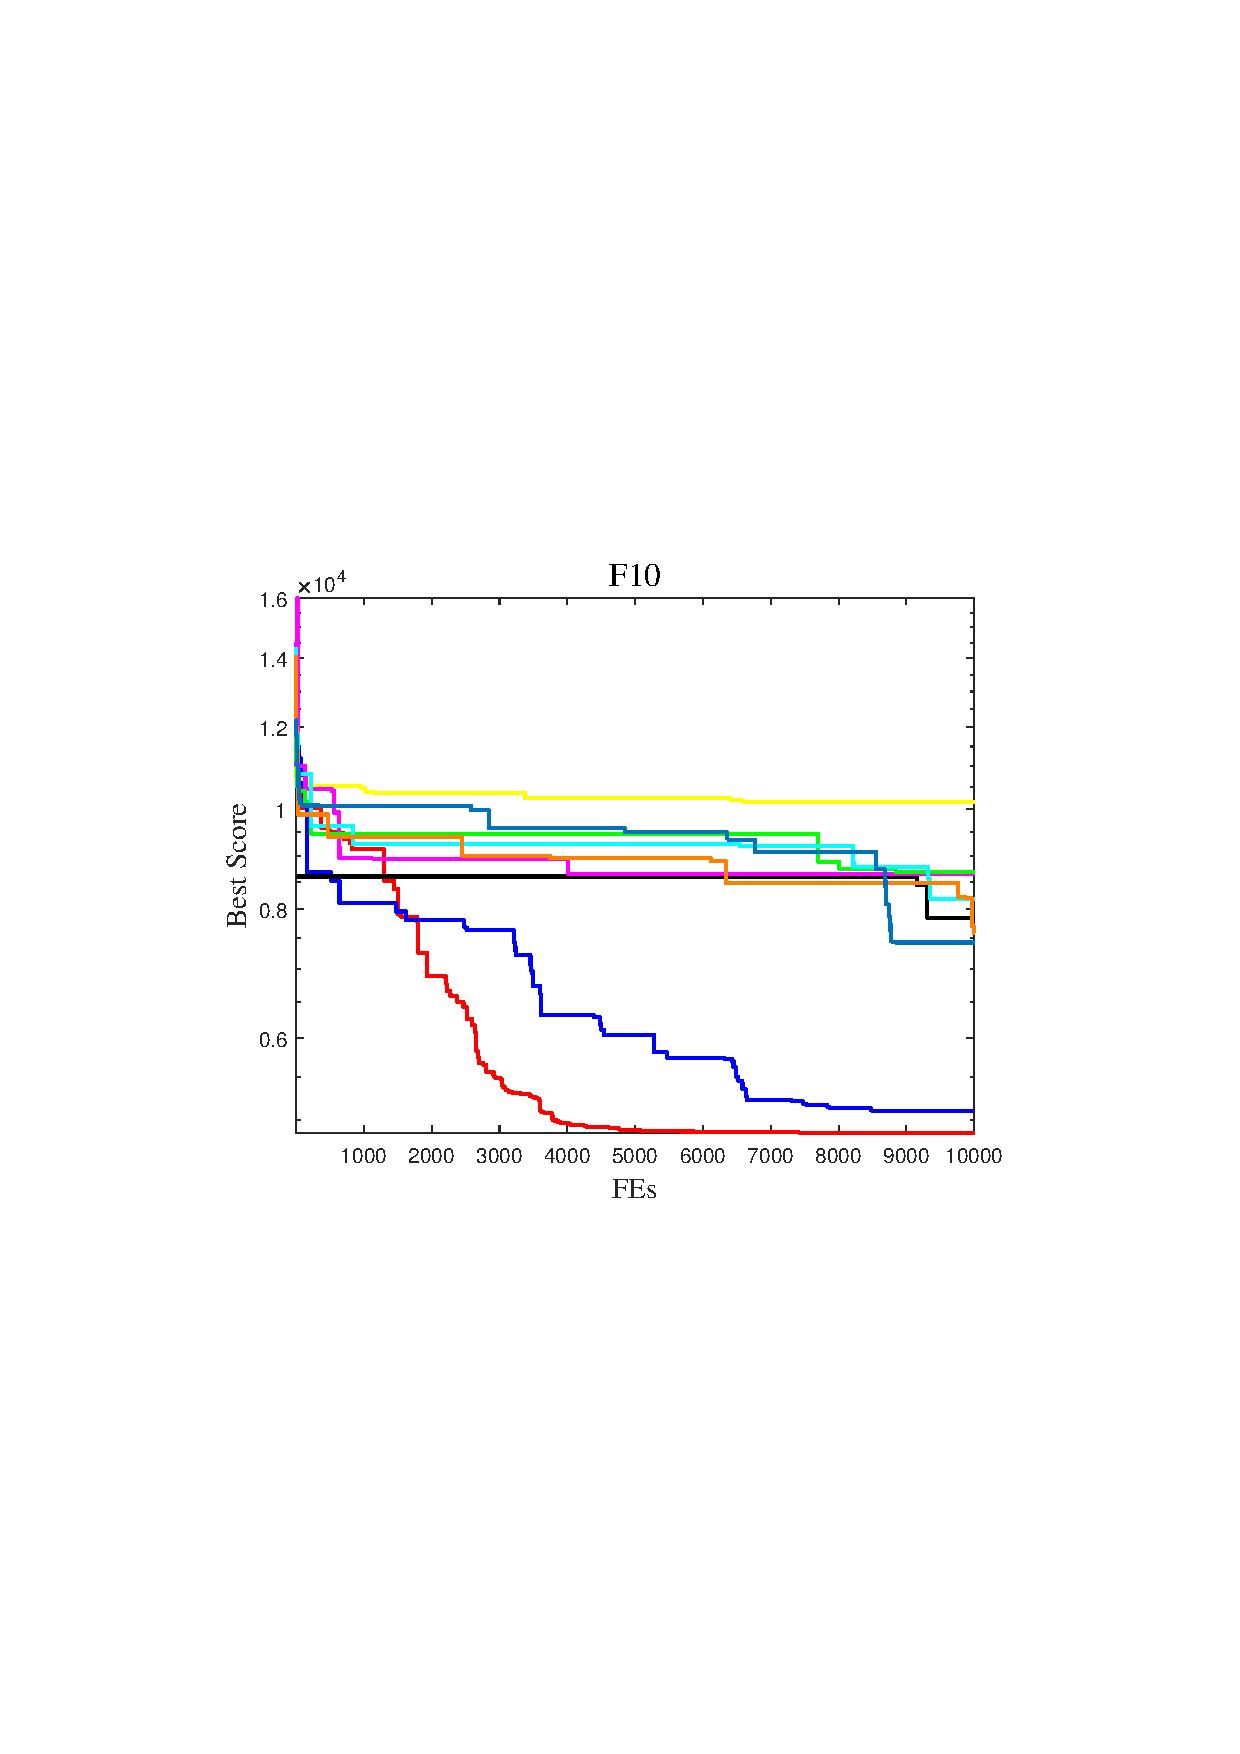
\includegraphics[width=\textwidth]{figures/Convergence/dim30/10.pdf}
    \end{subfigure}
    \hfill
    \begin{subfigure}[b]{0.32\textwidth}
        \caption*{}
        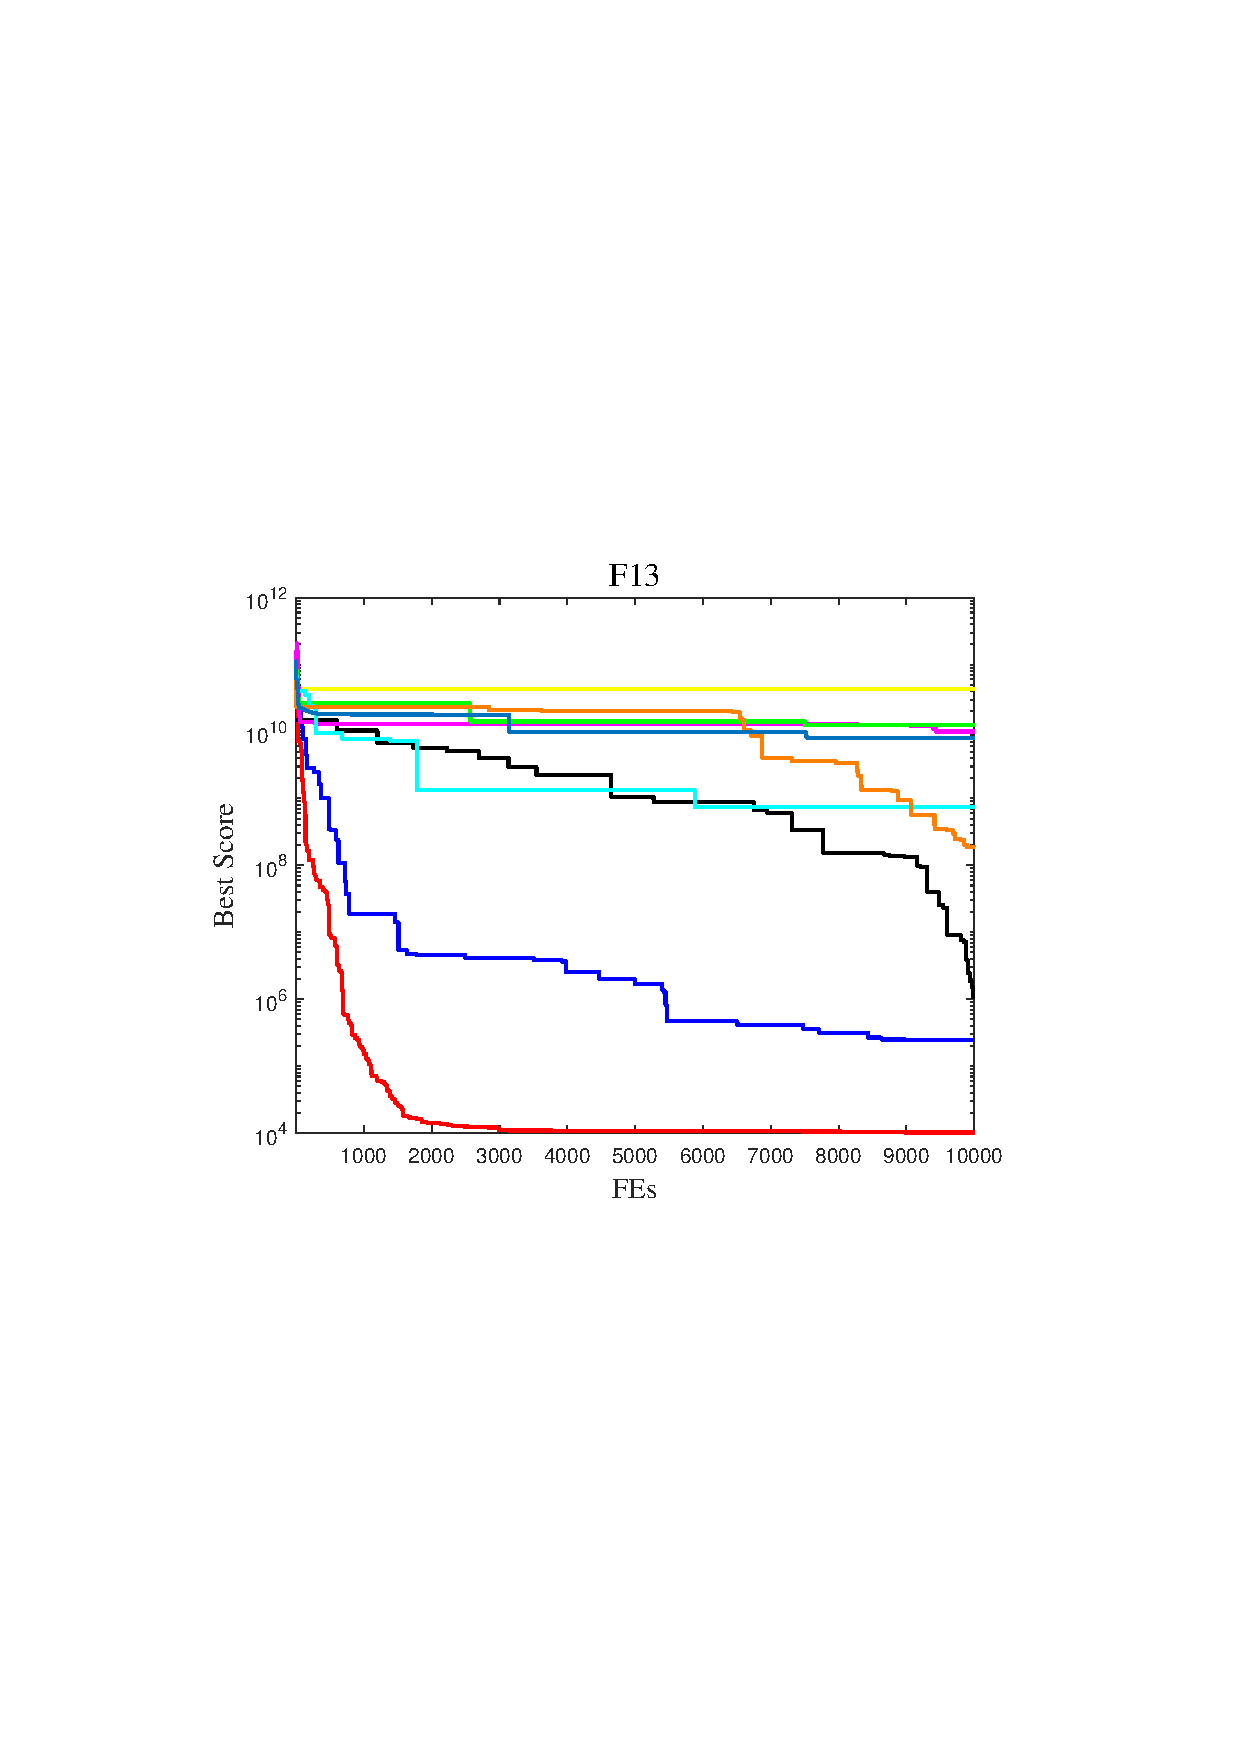
\includegraphics[width=\textwidth]{figures/Convergence/dim30/13.pdf}
    \end{subfigure}
    % 第三行子图
    \begin{subfigure}[b]{0.32\textwidth}
        \caption*{}
        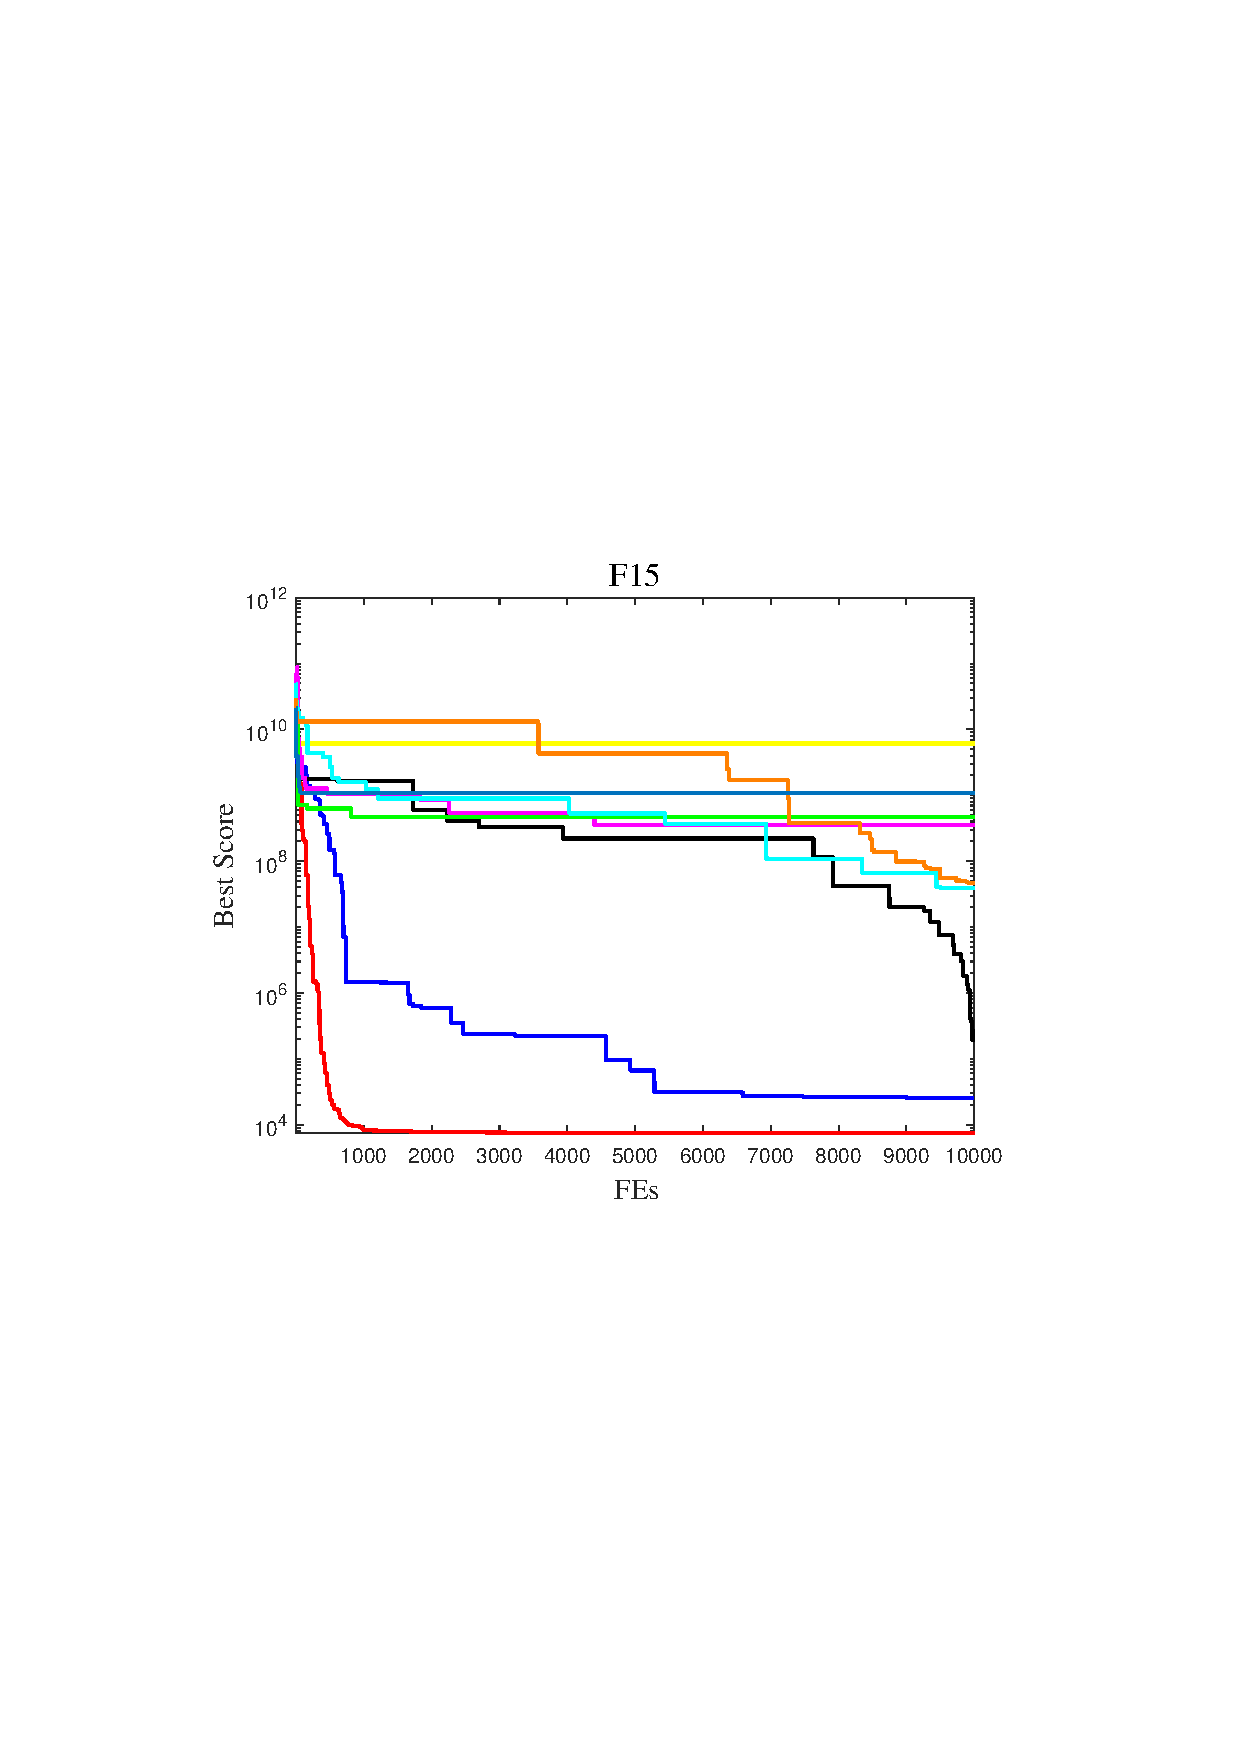
\includegraphics[width=\textwidth]{figures/Convergence/dim30/15.pdf}
    \end{subfigure}
    \hfill
    \begin{subfigure}[b]{0.32\textwidth}
        \caption*{}
        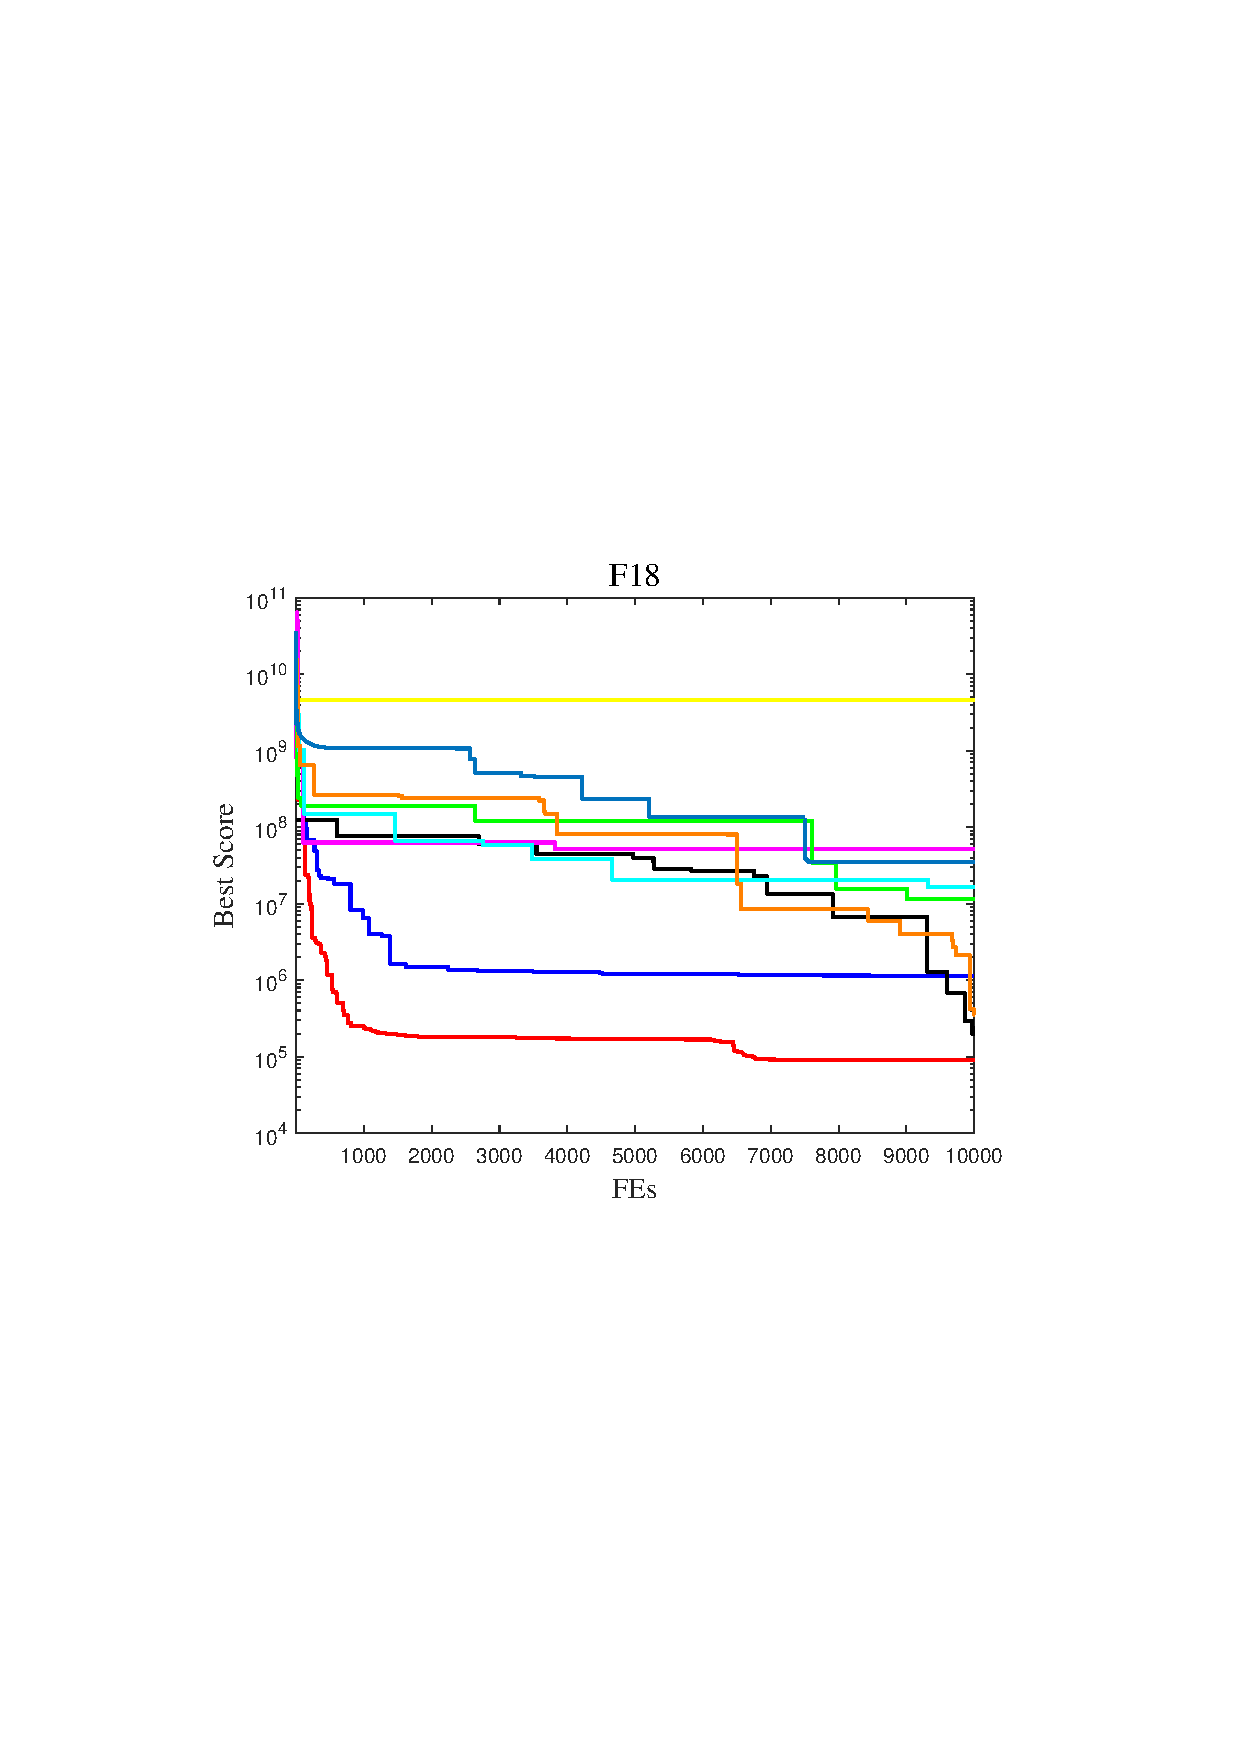
\includegraphics[width=\textwidth]{figures/Convergence/dim30/18.pdf}
    \end{subfigure}
    \hfill
    \begin{subfigure}[b]{0.32\textwidth}
        \caption*{}
        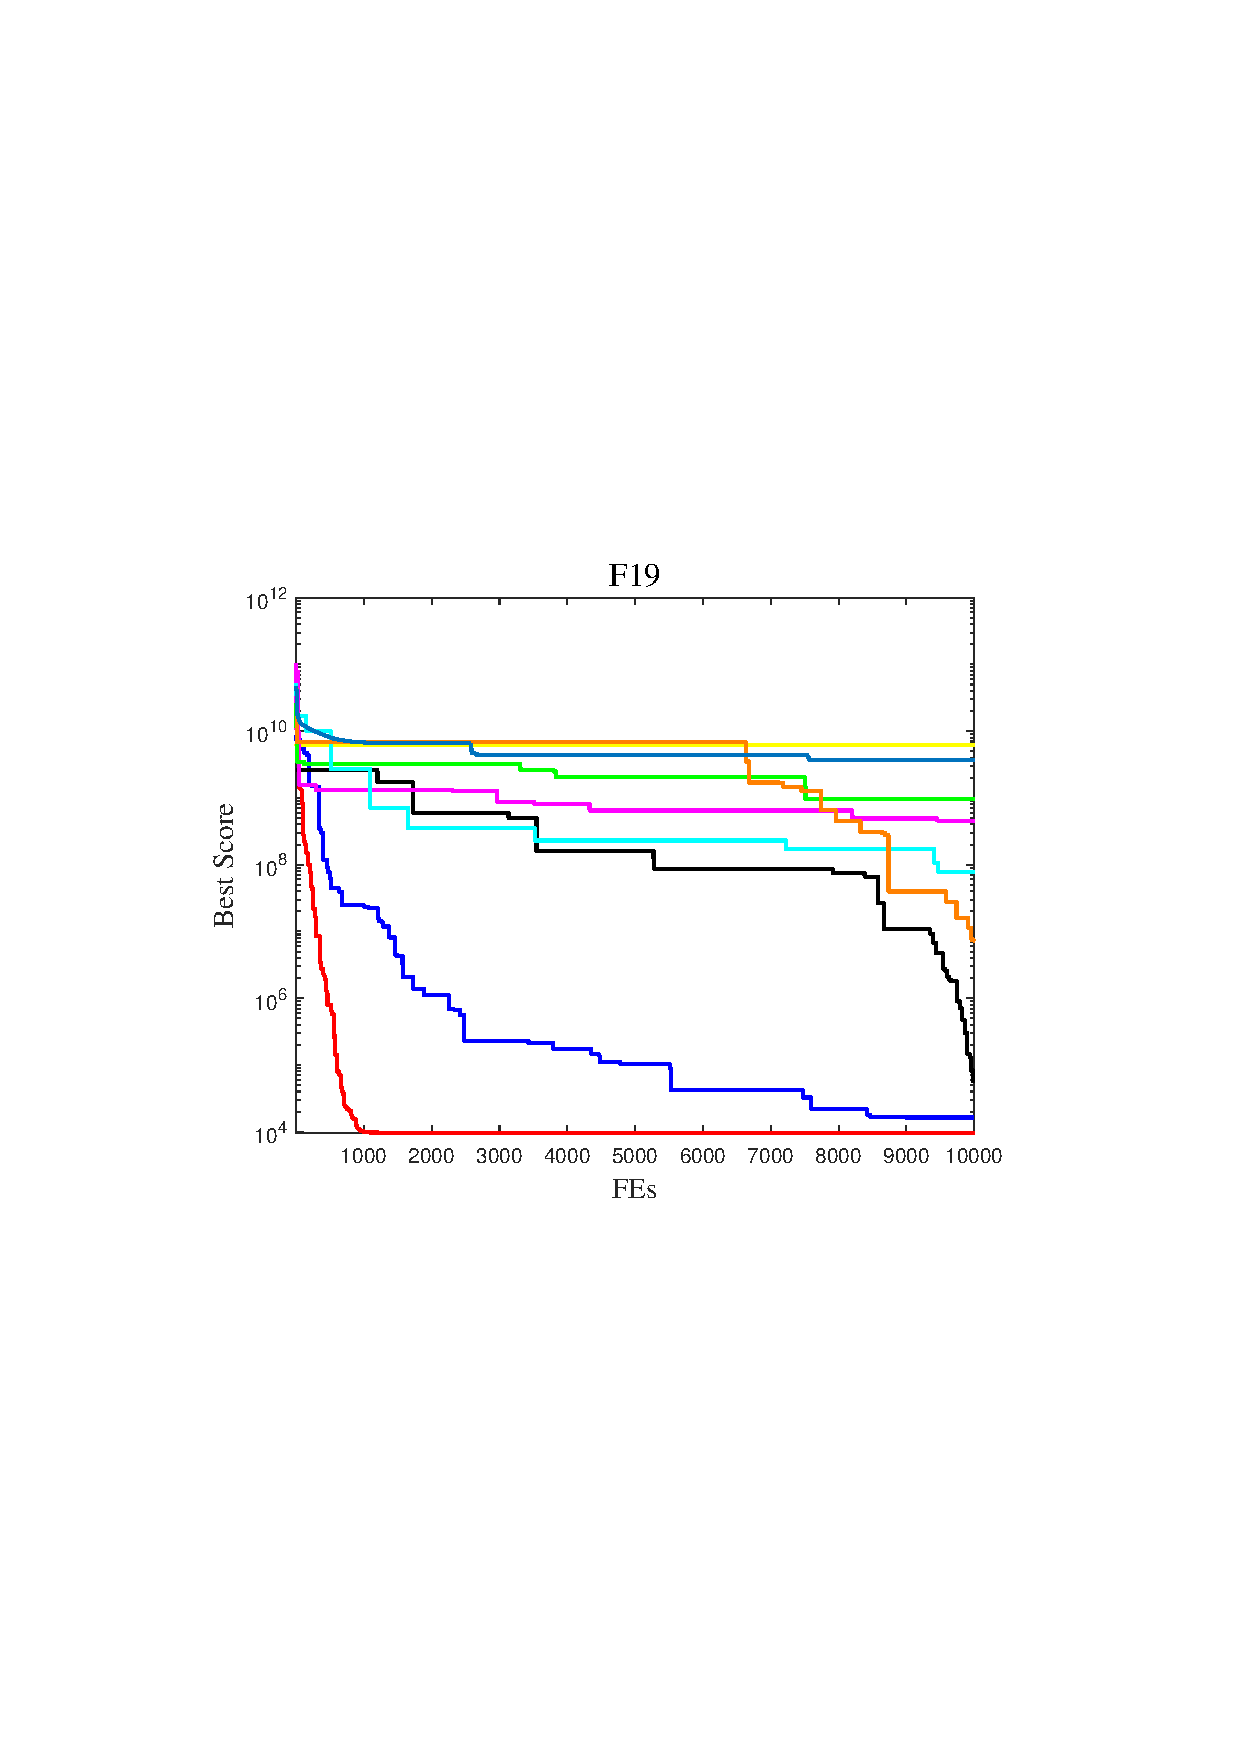
\includegraphics[width=\textwidth]{figures/Convergence/dim30/19.pdf}
    \end{subfigure}
    % 第四行（剩余3个子图，示例用F4,F5,F7）
    \begin{subfigure}[b]{0.32\textwidth}
        \caption*{}
        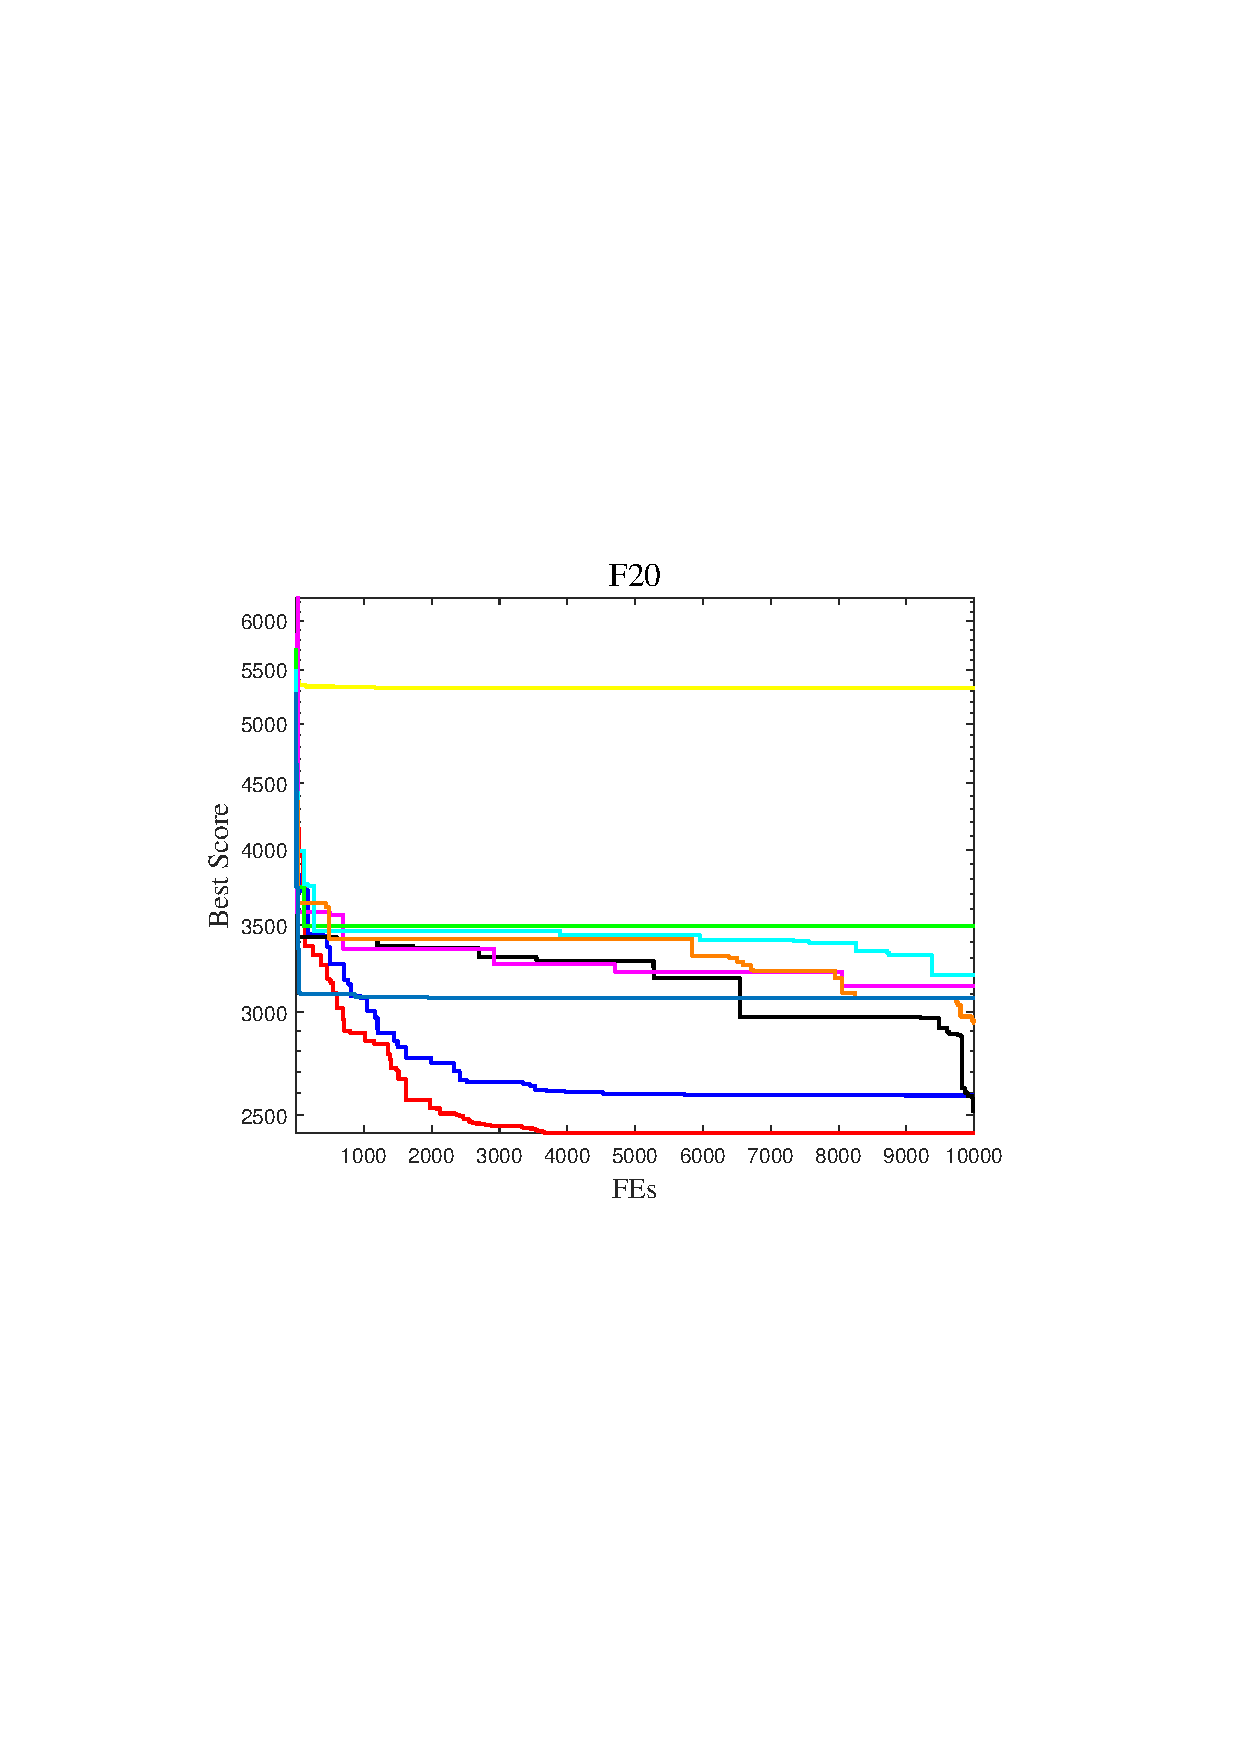
\includegraphics[width=\textwidth]{figures/Convergence/dim30/20.pdf}
    \end{subfigure}
    \hfill
    \begin{subfigure}[b]{0.32\textwidth}
        \caption*{}
        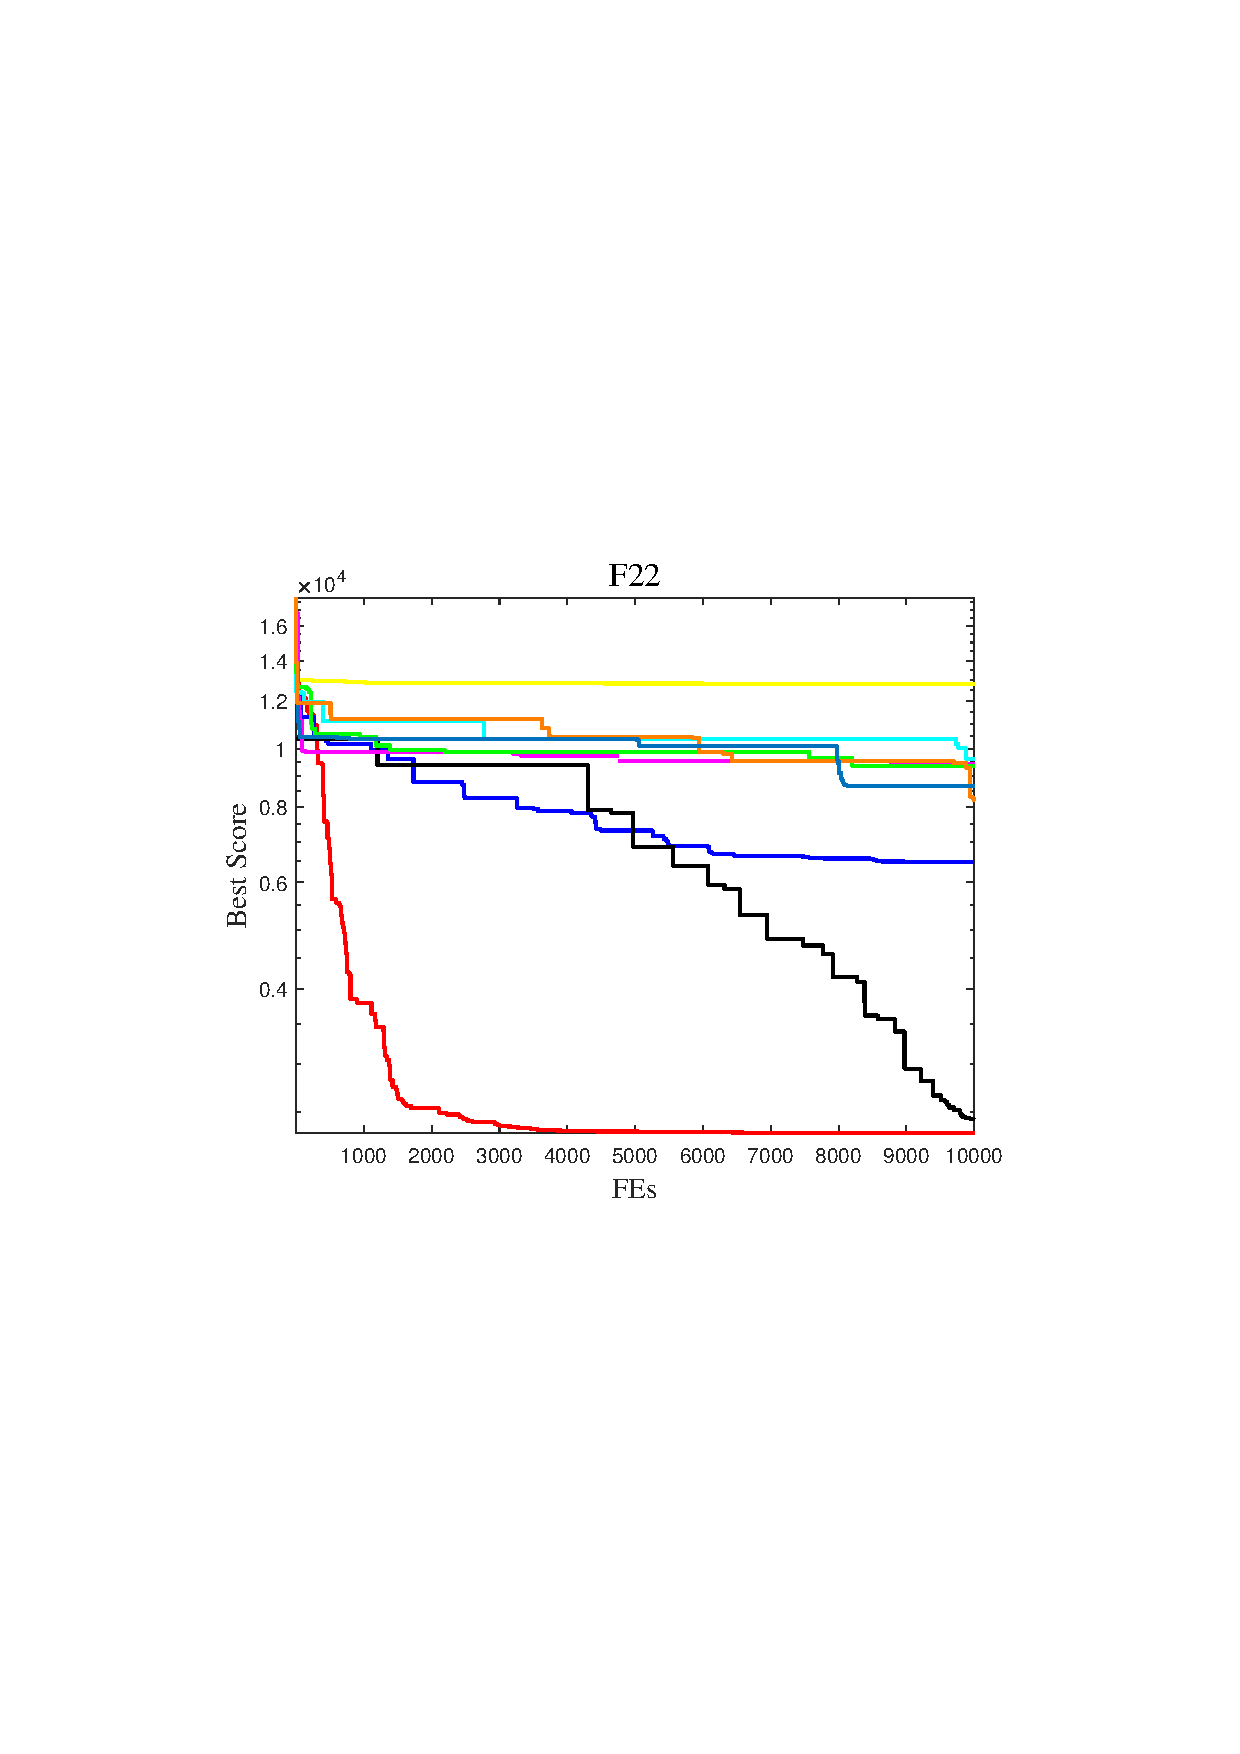
\includegraphics[width=\textwidth]{figures/Convergence/dim30/22.pdf}
    \end{subfigure}
    \hfill
    \begin{subfigure}[b]{0.32\textwidth}
        \caption*{}
        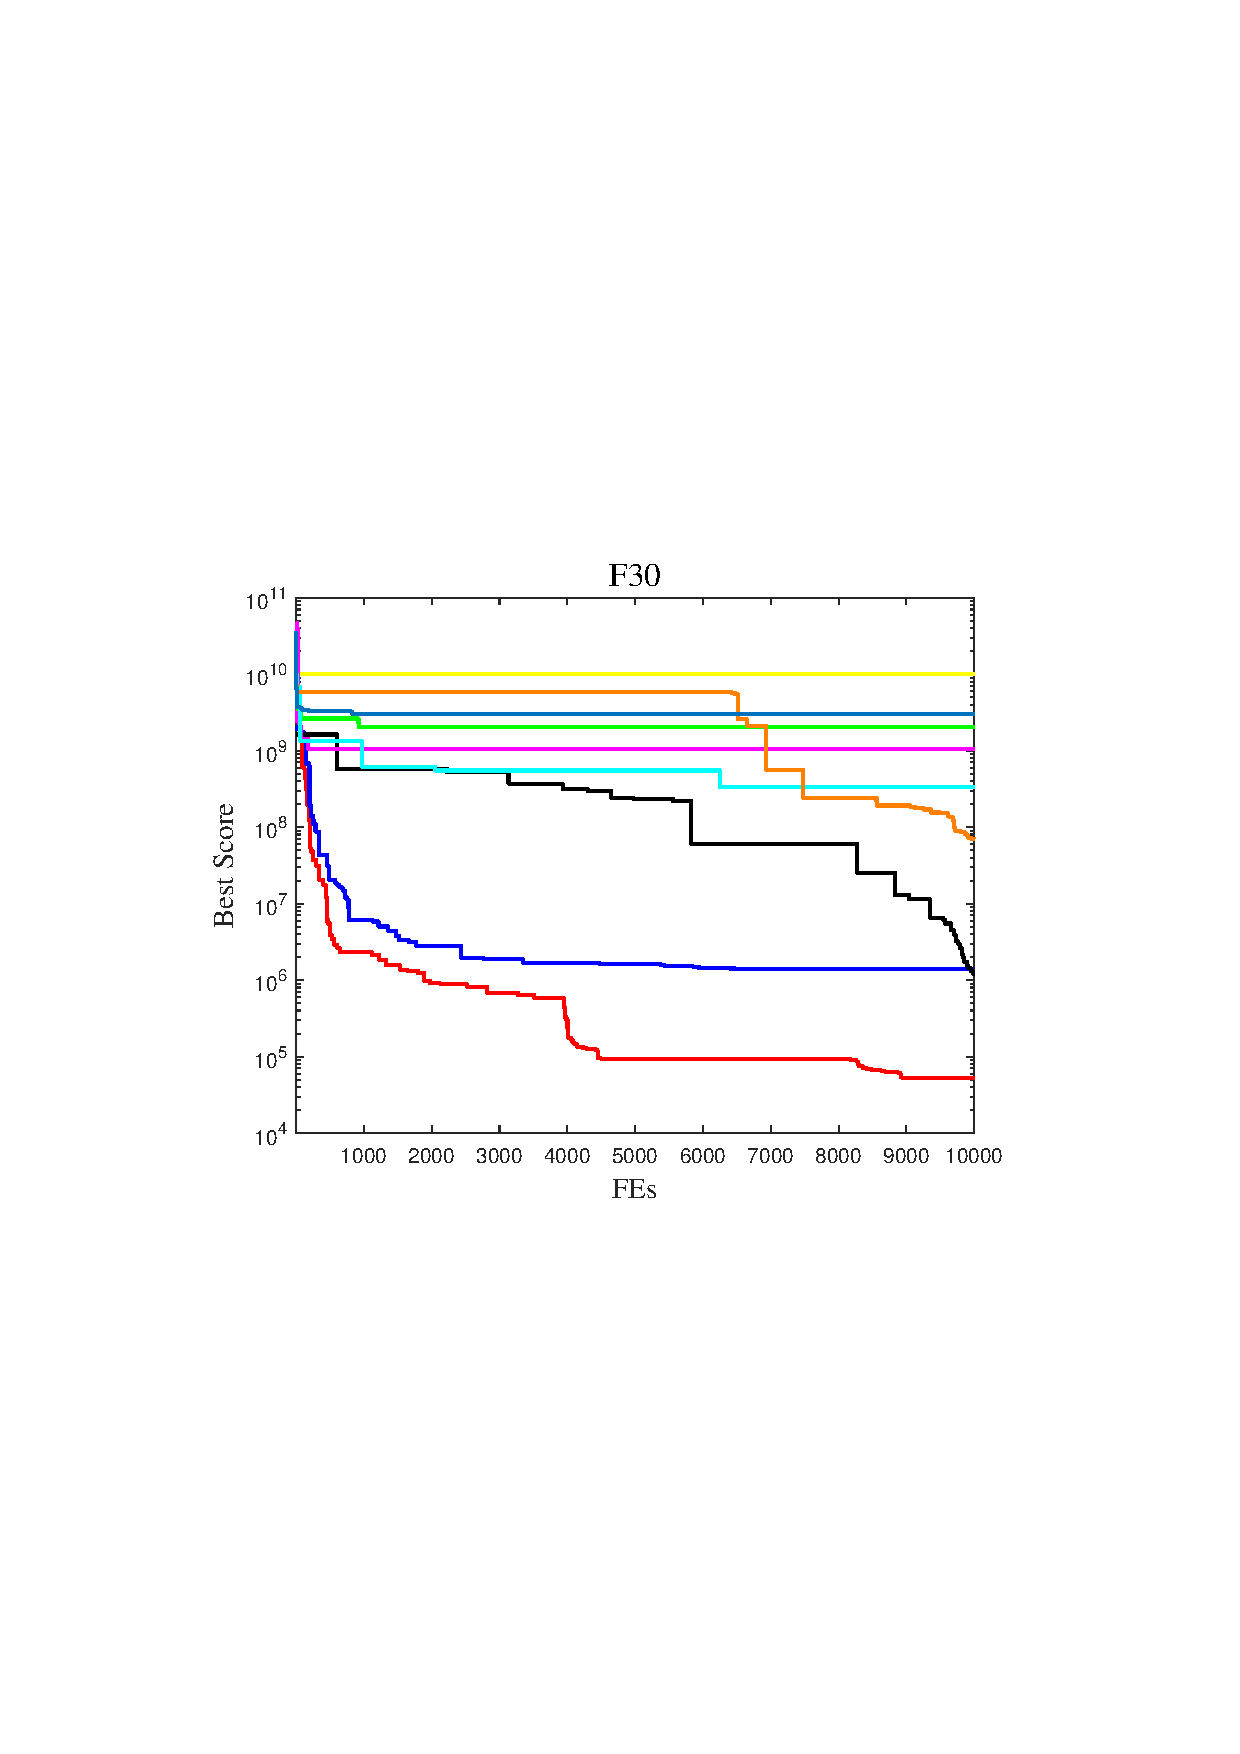
\includegraphics[width=\textwidth]{figures/Convergence/dim30/30.pdf}
    \end{subfigure}
    % 插入单独图例图片（宽度建议设为子图宽度的2/3）
    \vspace{0.5cm}
    \includegraphics[width=0.5\textwidth]{figures/Convergence/dim30/legend.pdf}
    \bicaption{12 个基准函数上的收敛曲线 (30D)}{Convergence curves on the 12 benchmark functions (30D)}
    \label{fig:curve-dim30}
\end{figure}

% 50维曲线图
\begin{figure}[htbp]
    \centering
    % 第一行子图 (F1, F2, F3)
    \begin{subfigure}[b]{0.32\textwidth}
        \caption*{}
        
\includegraphics[width=\textwidth]{figures/Convergence/dim50/1.pdf}
    \end{subfigure}
    \hfill
    \begin{subfigure}[b]{0.32\textwidth}
        \caption*{}
        
\includegraphics[width=\textwidth]{figures/Convergence/dim50/5.pdf}
    \end{subfigure}
    \hfill
    \begin{subfigure}[b]{0.32\textwidth}
        \caption*{}
        
\includegraphics[width=\textwidth]{figures/Convergence/dim50/6.pdf}
    \end{subfigure}
    % 第二行子图 (F6, F11, F16)
    \begin{subfigure}[b]{0.32\textwidth}
        \caption*{}
        
\includegraphics[width=\textwidth]{figures/Convergence/dim50/8.pdf}
    \end{subfigure}
    \hfill
    \begin{subfigure}[b]{0.32\textwidth}
        \caption*{}
        
\includegraphics[width=\textwidth]{figures/Convergence/dim50/10.pdf}
    \end{subfigure}
    \hfill
    \begin{subfigure}[b]{0.32\textwidth}
        \caption*{}
        
\includegraphics[width=\textwidth]{figures/Convergence/dim50/13.pdf}
    \end{subfigure}
    % 第三行子图
    \begin{subfigure}[b]{0.32\textwidth}
        \caption*{}
        
\includegraphics[width=\textwidth]{figures/Convergence/dim50/15.pdf}
    \end{subfigure}
    \hfill
    \begin{subfigure}[b]{0.32\textwidth}
        \caption*{}
        
\includegraphics[width=\textwidth]{figures/Convergence/dim50/18.pdf}
    \end{subfigure}
    \hfill
    \begin{subfigure}[b]{0.32\textwidth}
        \caption*{}
        
\includegraphics[width=\textwidth]{figures/Convergence/dim50/19.pdf}
    \end{subfigure}
    % 第四行（剩余3个子图，示例用F4,F5,F7）
    \begin{subfigure}[b]{0.32\textwidth}
        \caption*{}
        
\includegraphics[width=\textwidth]{figures/Convergence/dim50/20.pdf}
    \end{subfigure}
    \hfill
    \begin{subfigure}[b]{0.32\textwidth}
        \caption*{}
        
\includegraphics[width=\textwidth]{figures/Convergence/dim50/22.pdf}
    \end{subfigure}
    \hfill
    \begin{subfigure}[b]{0.32\textwidth}
        \caption*{}
        
\includegraphics[width=\textwidth]{figures/Convergence/dim50/30.pdf}
    \end{subfigure}
    % 插入单独图例图片（宽度建议设为子图宽度的2/3）
    \vspace{0.5cm}
    \includegraphics[width=0.5\textwidth]{figures/Convergence/dim30/legend.pdf}
    \bicaption{12 个基准函数上的收敛曲线 (50D)}{Convergence curves on the 12 benchmark functions (50D)}
    \label{fig:curve-dim50}
\end{figure}

\subsubsection{箱线图分析}
图 6 和图 7 分别展示了 30 维和 50 维的箱线图。在大多数基准函数中，IRIME 的箱线图始终显示出较低的中位数和较窄的四分位距，表明其性能更好且更稳定。例如，在 F1 函数中，IRIME 的中位数结果远低于 RIME 和 LSHADE 等竞争算法，这表明 IRIME 能更稳定地收敛到更优解。此外，其较小的四分位距表明结果的离散度较低，反映出高稳定性。在高维的 F4 函数中，IRIME 也表现出色，其箱线图的整体位置低于大多数其他算法，进一步证明了其在复杂高维环境中进行高效优化的能力。此外，在不同的基准函数中，IRIME 的箱线图始终表现出类似的优势特征，而一些算法（如 BDA 和 RIME）在多个函数中表现不佳，表现为中位数较高或离散度较大。总体而言，IRIME 在 CEC 2017 基准测试集上表现出强大的优化性能和稳健的稳定性，在低维和高维情况下均表现出色。这些结果凸显了其与其他竞争算法相比的明显优势。

% 30维箱型图
\begin{figure}[htbp]
    \centering
    % 第一行子图
    \begin{subfigure}[b]{0.32\textwidth}
        \caption*{}
        
\includegraphics[width=\textwidth]{figures/box/dim30/1.pdf}
    \end{subfigure}
    \hfill
    \begin{subfigure}[b]{0.32\textwidth}
        \caption*{}
        
\includegraphics[width=\textwidth]{figures/box/dim30/5.pdf}
    \end{subfigure}
    \hfill
    \begin{subfigure}[b]{0.32\textwidth}
        \caption*{}
        
\includegraphics[width=\textwidth]{figures/box/dim30/6.pdf}
    \end{subfigure}
    % 第二行子图
    \begin{subfigure}[b]{0.32\textwidth}
        \caption*{}
        
\includegraphics[width=\textwidth]{figures/box/dim30/8.pdf}
    \end{subfigure}
    \hfill
    \begin{subfigure}[b]{0.32\textwidth}
        \caption*{}
        
\includegraphics[width=\textwidth]{figures/box/dim30/10.pdf}
    \end{subfigure}
    \hfill
    \begin{subfigure}[b]{0.32\textwidth}
        \caption*{}
        
\includegraphics[width=\textwidth]{figures/box/dim30/13.pdf}
    \end{subfigure}
    % 第三行子图
    \begin{subfigure}[b]{0.32\textwidth}
        \caption*{}
        
\includegraphics[width=\textwidth]{figures/box/dim30/15.pdf}
    \end{subfigure}
    \hfill
    \begin{subfigure}[b]{0.32\textwidth}
        \caption*{}
        
\includegraphics[width=\textwidth]{figures/box/dim30/18.pdf}
    \end{subfigure}
    \hfill
    \begin{subfigure}[b]{0.32\textwidth}
        \caption*{}
        
\includegraphics[width=\textwidth]{figures/box/dim30/19.pdf}
    \end{subfigure}
    % 第四行
    \begin{subfigure}[b]{0.32\textwidth}
        \caption*{}
        
\includegraphics[width=\textwidth]{figures/box/dim30/20.pdf}
    \end{subfigure}
    \hfill
    \begin{subfigure}[b]{0.32\textwidth}
        \caption*{}
        
\includegraphics[width=\textwidth]{figures/box/dim30/22.pdf}
    \end{subfigure}
    \hfill
    \begin{subfigure}[b]{0.32\textwidth}
        \caption*{}
        
\includegraphics[width=\textwidth]{figures/box/dim30/30.pdf}
    \end{subfigure}
    \caption{12 个基准函数上的箱线图 (30D)}
    \label{fig:box-dim30}
\end{figure}
% 50维箱型图
\begin{figure}[htbp]
    \centering
    % 第一行子图
    \begin{subfigure}[b]{0.32\textwidth}
        \caption*{}
        
\includegraphics[width=\textwidth]{figures/box/dim50/1.pdf}
    \end{subfigure}
    \hfill
    \begin{subfigure}[b]{0.32\textwidth}
        \caption*{}
        
\includegraphics[width=\textwidth]{figures/box/dim50/5.pdf}
    \end{subfigure}
    \hfill
    \begin{subfigure}[b]{0.32\textwidth}
        \caption*{}
        
\includegraphics[width=\textwidth]{figures/box/dim50/6.pdf}
    \end{subfigure}
    % 第二行子图
    \begin{subfigure}[b]{0.32\textwidth}
        \caption*{}
        
\includegraphics[width=\textwidth]{figures/box/dim50/8.pdf}
    \end{subfigure}
    \hfill
    \begin{subfigure}[b]{0.32\textwidth}
        \caption*{}
        
\includegraphics[width=\textwidth]{figures/box/dim50/10.pdf}
    \end{subfigure}
    \hfill
    \begin{subfigure}[b]{0.32\textwidth}
        \caption*{}
        
\includegraphics[width=\textwidth]{figures/box/dim50/13.pdf}
    \end{subfigure}
    % 第三行子图
    \begin{subfigure}[b]{0.32\textwidth}
        \caption*{}
        
\includegraphics[width=\textwidth]{figures/box/dim50/15.pdf}
    \end{subfigure}
    \hfill
    \begin{subfigure}[b]{0.32\textwidth}
        \caption*{}
        
\includegraphics[width=\textwidth]{figures/box/dim50/18.pdf}
    \end{subfigure}
    \hfill
    \begin{subfigure}[b]{0.32\textwidth}
        \caption*{}
        
\includegraphics[width=\textwidth]{figures/box/dim50/19.pdf}
    \end{subfigure}
    % 第四行
    \begin{subfigure}[b]{0.32\textwidth}
        \caption*{}
        
\includegraphics[width=\textwidth]{figures/box/dim50/20.pdf}
    \end{subfigure}
    \hfill
    \begin{subfigure}[b]{0.32\textwidth}
        \caption*{}
        
\includegraphics[width=\textwidth]{figures/box/dim50/22.pdf}
    \end{subfigure}
    \hfill
    \begin{subfigure}[b]{0.32\textwidth}
        \caption*{}
        
\includegraphics[width=\textwidth]{figures/box/dim50/30.pdf}
    \end{subfigure}
    \bicaption{12 个基准函数上的箱线图 (50D)}{Boxplots on the 12 benchmark functions}
    \label{fig:box-dim50}
\end{figure}

\subsubsection{弗里德曼统计检验}
CEC 2017 的弗里德曼统计结果表明，所提出的算法具有明显优势。在 30 维测试中，IRIME 在大多数函数（如 F1、F3、F5）上获得了顶级排名，最终总排名为 1.31，如图 5 所示，显著优于 BDA（排名：9.00）等算法。同样，在 50 维测试中，它在多个函数（如 F1、F4、F11）上表现出色，总排名为 1.21，超过了大多数竞争对手。值得注意的是，IRIME 在不同维度上始终保持高性能，而像 BDA 这样的算法在大多数情况下排名较差。这些结果强调了我们的算法在 CEC 2017 测试集上具有卓越的优化能力，能够提供更稳定、更准确的解，并具有显著的性能优势。

\begin{figure}[htbp]
    \centering
    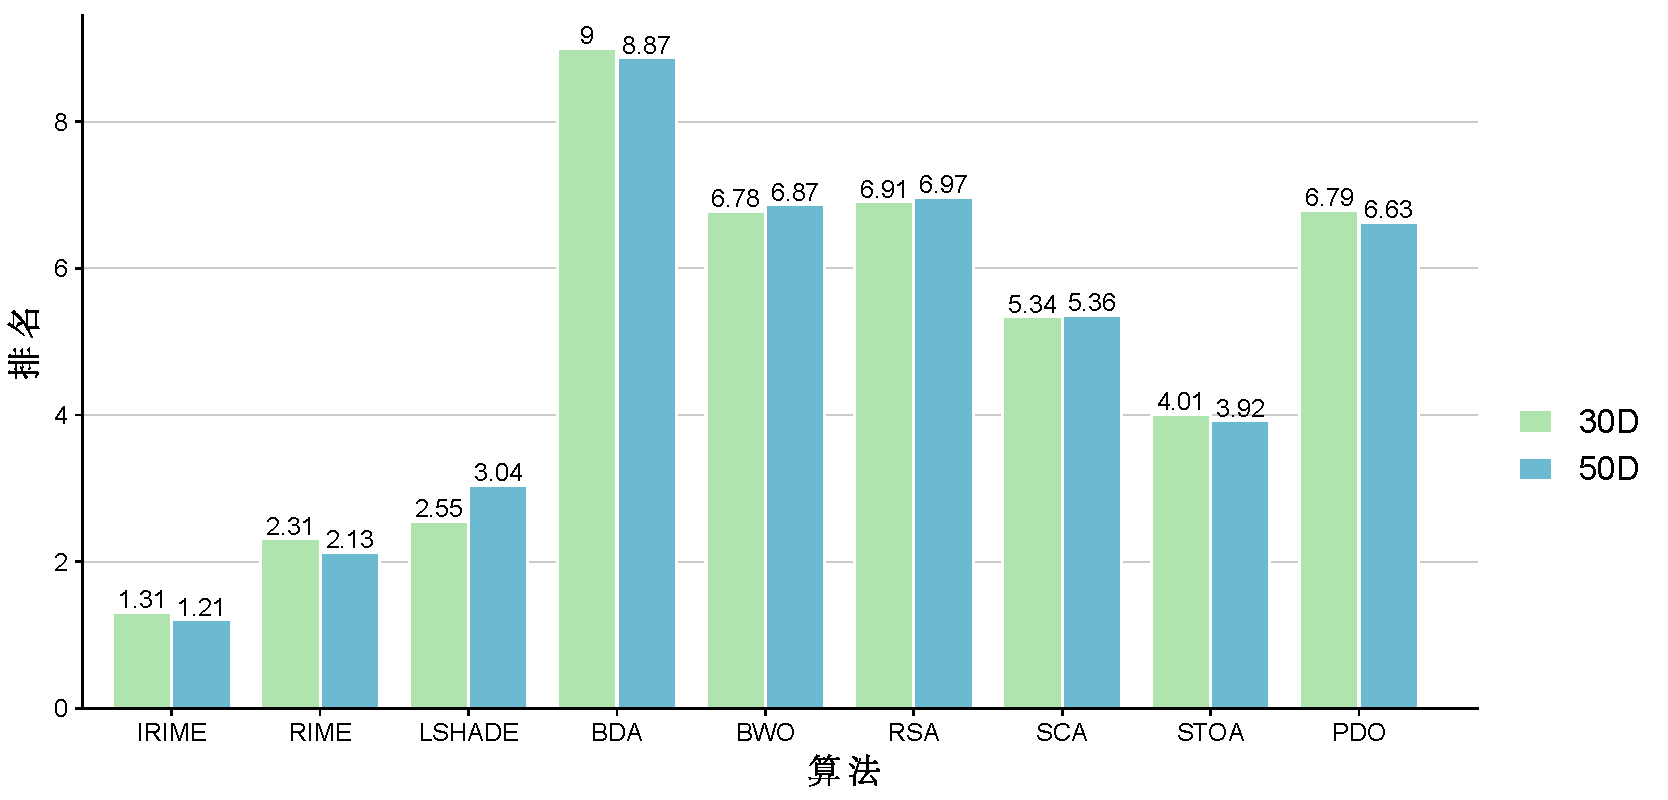
\includegraphics[width=0.8\linewidth]{figures/Ftest/Ftest-dim30-dim50.pdf} % 调整宽度为适合您文档的值
    \bicaption{九种算法的弗里德曼检验结果 (30D)}{Friedman test results for the nine algorithms}
    \label{fig:Ftest-dim30-dim50}
\end{figure}

% Table generated by Excel2LaTeX from sheet 'dim=30'
\begin{table}[htbp]
  \centering
  \caption{九种算法在 CEC 2017 函数上的对比结果 (30D)}
    \setlength{\tabcolsep}{3pt} % 减少列间距
    \tiny
    \begin{tabular}{ccccccccccc}
    \toprule    
    Function & Metric & IRIME & RIME  & LSHADE & BDA   & BWO   & RSA   & SCA   & STOA  & PDO \\
    \midrule
    \multirow{3}[0]{*}{F1} & best  & \textbf{3.9536E+02} & 5.2647E+06 & 5.4242E+07 & 8.3562E+10 & 3.7651E+10 & 4.2848E+10 & 1.7636E+10 & 4.5851E+09 & 3.7472E+10 \\
          & mean  & \textbf{1.2630E+04} & 1.1814E+07 & 1.4184E+08 & 8.3562E+10 & 5.3274E+10 & 5.1575E+10 & 2.1336E+10 & 9.9804E+09 & 5.1169E+10 \\
          & std   & \textbf{1.8998E+04} & 8.0266E+06 & 5.1258E+07 & 1.2458E+06 & 6.8511E+09 & 5.6243E+09 & 2.5245E+09 & 4.8163E+09 & 8.7213E+09 \\
    \multirow{3}[0]{*}{F3} & best  & \textbf{8.2299E+03} & 3.6361E+04 & 2.6980E+04 & 2.0708E+08 & 8.1210E+04 & 7.8591E+04 & 6.6386E+04 & 5.3102E+04 & 7.2520E+04 \\
          & mean  & \textbf{2.1615E+04} & 8.3219E+04 & 5.3301E+04 & 2.0711E+08 & 8.5214E+04 & 8.4359E+04 & 9.6629E+04 & 8.6975E+04 & 9.3874E+04 \\
          & std   & 9.4119E+03 & 2.5552E+04 & 3.0814E+04 & 7.1537E+04 & \textbf{3.5034E+03} & 4.3231E+03 & 1.7633E+04 & 1.6677E+04 & 9.5676E+03 \\
    \multirow{3}[0]{*}{F4} & best  & 4.7010E+02 & \textbf{4.5622E+02} & 5.1476E+02 & 3.3625E+04 & 8.5256E+03 & 7.0539E+03 & 1.9858E+03 & 7.1457E+02 & 1.2573E+04 \\
          & mean  & \textbf{5.1668E+02} & 5.2012E+02 & 5.3046E+02 & 3.3626E+04 & 1.3771E+04 & 1.2903E+04 & 3.4697E+03 & 1.0213E+03 & 1.7112E+04 \\
          & std   & 4.1599E+01 & 2.8219E+01 & 1.2024E+01 & \textbf{3.0273E+00} & 2.3685E+03 & 4.6584E+03 & 1.5641E+03 & 2.0769E+02 & 3.2391E+03 \\
    \multirow{3}[0]{*}{F5} & best  & \textbf{5.3285E+02} & 5.8377E+02 & 6.6955E+02 & 1.0973E+03 & 9.0328E+02 & 8.5311E+02 & 7.8762E+02 & 6.8542E+02 & 8.2716E+02 \\
          & mean  & \textbf{5.9967E+02} & 6.4155E+02 & 6.9952E+02 & 1.0974E+03 & 9.4670E+02 & 9.3248E+02 & 8.2124E+02 & 7.3588E+02 & 8.8312E+02 \\
          & std   & 3.6243E+01 & 3.7195E+01 & 2.0194E+01 & \textbf{1.9435E-01} & 1.8460E+01 & 3.5877E+01 & 1.9560E+01 & 3.1438E+01 & 4.8352E+01 \\
    \multirow{3}[0]{*}{F6} & best  & \textbf{6.0493E+02} & 6.0643E+02 & 6.0761E+02 & 7.2477E+02 & 6.8612E+02 & 6.8537E+02 & 6.5310E+02 & 6.3957E+02 & 6.7747E+02 \\
          & mean  & 6.1517E+02 & 6.1974E+02 & \textbf{6.1173E+02} & 7.2479E+02 & 6.9374E+02 & 6.9430E+02 & 6.6231E+02 & 6.4952E+02 & 6.9153E+02 \\
          & std   & 7.8417E+00 & 1.0925E+01 & 2.5890E+00 & \textbf{6.6924E-02} & 4.9400E+00 & 6.0931E+00 & 7.3655E+00 & 6.7059E+00 & 9.4765E+00 \\
    \multirow{3}[0]{*}{F7} & best  & \textbf{7.8787E+02} & 8.4285E+02 & 9.2850E+02 & 1.5434E+03 & 1.3857E+03 & 1.2815E+03 & 1.1524E+03 & 1.0123E+03 & 1.2566E+03 \\
          & mean  & \textbf{8.5071E+02} & 8.9660E+02 & 9.5193E+02 & 1.5443E+03 & 1.4315E+03 & 1.3797E+03 & 1.2656E+03 & 1.1486E+03 & 1.3793E+03 \\
          & std   & 2.5417E+01 & 4.9745E+01 & 1.4056E+01 & \textbf{1.5374E+00} & 2.8622E+01 & 4.2492E+01 & 8.1489E+01 & 7.0323E+01 & 9.7185E+01 \\
    \multirow{3}[0]{*}{F8} & best  & \textbf{8.4677E+02} & 8.9139E+02 & 9.6323E+02 & 1.2873E+03 & 1.1246E+03 & 1.1000E+03 & 1.0598E+03 & 9.3904E+02 & 1.0749E+03 \\
          & mean  & \textbf{8.8877E+02} & 9.1929E+02 & 1.0021E+03 & 1.2873E+03 & 1.1437E+03 & 1.1420E+03 & 1.0979E+03 & 9.8960E+02 & 1.1274E+03 \\
          & std   & 2.9069E+01 & 2.8160E+01 & 1.6297E+01 & \textbf{0.0000E+00} & 1.2953E+01 & 2.8423E+01 & 2.1894E+01 & 2.8649E+01 & 2.2616E+01 \\
    \multirow{3}[0]{*}{F9} & best  & \textbf{1.0263E+03} & 2.3289E+03 & 1.1155E+03 & 1.4602E+04 & 1.0199E+04 & 1.0589E+04 & 5.5744E+03 & 3.5410E+03 & 7.0386E+03 \\
          & mean  & 1.8441E+03 & 3.3495E+03 & \textbf{1.2633E+03} & 1.5113E+04 & 1.1876E+04 & 1.1840E+04 & 8.6730E+03 & 6.3974E+03 & 9.0529E+03 \\
          & std   & 5.2798E+02 & 8.3314E+02 & \textbf{1.0928E+02} & 4.9105E+02 & 8.4573E+02 & 8.0193E+02 & 3.6398E+03 & 1.7711E+03 & 1.5880E+03 \\
    \multirow{3}[0]{*}{F10} & best  & 4.0571E+03 & \textbf{3.5667E+03} & 6.7934E+03 & 1.0152E+04 & 8.1524E+03 & 7.8404E+03 & 8.2932E+03 & 7.0094E+03 & 7.0747E+03 \\
          & mean  & \textbf{4.9052E+03} & 5.0016E+03 & 7.6695E+03 & 1.0152E+04 & 8.8377E+03 & 8.5623E+03 & 9.0177E+03 & 7.8949E+03 & 8.4293E+03 \\
          & std   & 5.0523E+02 & 8.1336E+02 & 5.7198E+02 & \textbf{1.9174E-12} & 3.3010E+02 & 4.0894E+02 & 3.5919E+02 & 4.9143E+02 & 6.6900E+02 \\
    \multirow{3}[0]{*}{F11} & best  & \textbf{1.1582E+03} & 1.3192E+03 & 1.3250E+03 & 6.0091E+08 & 7.0103E+03 & 7.9034E+03 & 3.3435E+03 & 1.8927E+03 & 8.4164E+03 \\
          & mean  & \textbf{1.2125E+03} & 1.4018E+03 & 1.4180E+03 & 6.0091E+08 & 8.5338E+03 & 1.2531E+04 & 4.5446E+03 & 3.1640E+03 & 1.5386E+04 \\
          & std   & 4.5204E+01 & 8.5198E+01 & 4.3547E+01 & \textbf{0.0000E+00} & 1.0129E+03 & 4.7695E+03 & 1.0827E+03 & 1.0173E+03 & 5.5635E+03 \\
    \multirow{3}[0]{*}{F12} & best  & \textbf{4.7278E+05} & 5.4646E+06 & 7.5373E+06 & 2.8660E+10 & 8.3002E+09 & 6.9339E+09 & 2.4024E+09 & 2.1009E+08 & 5.6626E+09 \\
          & mean  & \textbf{2.6792E+06} & 1.8208E+07 & 1.3654E+07 & 2.8660E+10 & 1.2638E+10 & 1.6219E+10 & 2.9259E+09 & 3.9737E+08 & 1.3528E+10 \\
          & std   & 2.2870E+06 & 1.1207E+07 & 4.9606E+06 & \textbf{0.0000E+00} & 2.1516E+09 & 4.3572E+09 & 4.3408E+08 & 2.4760E+08 & 3.2527E+09 \\
    \multirow{3}[0]{*}{F13} & best  & \textbf{2.3495E+03} & 4.4526E+04 & 3.8525E+05 & 4.2961E+10 & 6.0762E+09 & 4.9334E+09 & 5.1236E+08 & 1.6425E+07 & 8.7037E+09 \\
          & mean  & \textbf{1.5537E+04} & 3.6796E+05 & 8.9004E+05 & 4.2961E+10 & 8.8544E+09 & 1.1954E+10 & 1.5684E+09 & 1.7393E+08 & 1.2576E+10 \\
          & std   & 1.4965E+04 & 5.1697E+05 & 4.3333E+05 & \textbf{3.9480E+00} & 2.3263E+09 & 4.1107E+09 & 7.8094E+08 & 1.3380E+08 & 1.9560E+09 \\
    \multirow{3}[0]{*}{F14} & best  & 5.5721E+03 & 5.4723E+04 & \textbf{2.2293E+03} & 1.2163E+09 & 1.5717E+06 & 1.6764E+06 & 2.1133E+05 & 1.0611E+05 & 2.2498E+06 \\
          & mean  & 6.2927E+04 & 2.5410E+05 & \textbf{3.5509E+03} & 1.2163E+09 & 5.3556E+06 & 2.2099E+07 & 1.4880E+06 & 8.5560E+05 & 6.7811E+06 \\
          & std   & 4.9805E+04 & 1.7104E+05 & 1.6444E+03 & \textbf{2.9930E-01} & 3.9970E+06 & 2.2221E+07 & 1.6016E+06 & 1.0907E+06 & 4.6329E+06 \\
    \multirow{3}[0]{*}{F15} & best  & \textbf{1.5589E+03} & 3.9840E+03 & 4.2351E+04 & 6.1107E+09 & 8.1003E+07 & 2.8528E+08 & 8.9639E+06 & 3.4223E+05 & 5.5119E+07 \\
          & mean  & \textbf{2.5856E+03} & 3.2942E+04 & 7.6706E+04 & 6.1107E+09 & 3.9529E+08 & 8.2459E+08 & 6.2716E+07 & 4.1439E+07 & 4.9713E+08 \\
          & std   & 1.3341E+03 & 2.4738E+04 & 3.5047E+04 & \textbf{4.6460E-01} & 1.8894E+08 & 6.1038E+08 & 6.6251E+07 & 7.0899E+07 & 7.4038E+08 \\
    \multirow{3}[0]{*}{F16} & best  & \textbf{2.2792E+03} & 2.3688E+03 & 2.9531E+03 & 2.7095E+04 & 4.8615E+03 & 5.2683E+03 & 4.0189E+03 & 2.7343E+03 & 5.0818E+03 \\
          & mean  & \textbf{2.6996E+03} & 2.9473E+03 & 3.3655E+03 & 2.7099E+04 & 5.7998E+03 & 7.3134E+03 & 4.2636E+03 & 3.5017E+03 & 5.8756E+03 \\
          & std   & 2.7782E+02 & 3.0953E+02 & 2.9499E+02 & \textbf{8.3447E+00} & 4.6480E+02 & 1.8497E+03 & 2.1955E+02 & 5.3859E+02 & 5.6978E+02 \\
    \multirow{3}[0]{*}{F17} & best  & \textbf{1.9059E+03} & 1.9943E+03 & 2.1478E+03 & 2.5735E+05 & 3.3809E+03 & 3.3196E+03 & 2.7286E+03 & 2.0041E+03 & 3.2055E+03 \\
          & mean  & \textbf{2.2705E+03} & 2.3762E+03 & 2.2743E+03 & 2.5735E+05 & 4.4576E+03 & 7.4361E+03 & 2.9306E+03 & 2.5984E+03 & 3.9384E+03 \\
          & std   & 2.5405E+02 & 2.2414E+02 & 9.7950E+01 & \textbf{1.1148E-01} & 1.0298E+03 & 7.1610E+03 & 1.5843E+02 & 3.6943E+02 & 8.8913E+02 \\
    \multirow{3}[0]{*}{F18} & best  & 7.3706E+04 & 2.4634E+05 & \textbf{4.2999E+04} & 4.5513E+09 & 2.2342E+07 & 2.2292E+07 & 2.4640E+06 & 5.9727E+05 & 7.4076E+06 \\
          & mean  & 3.5254E+05 & 1.4304E+06 & \textbf{1.6788E+05} & 4.5513E+09 & 5.7045E+07 & 3.9039E+07 & 1.2933E+07 & 7.7296E+06 & 8.0185E+07 \\
          & std   & 2.7251E+05 & 1.0249E+06 & 1.5027E+05 & \textbf{1.9006E-01} & 3.0557E+07 & 1.7305E+07 & 6.9026E+06 & 8.5404E+06 & 3.3083E+07 \\
    \multirow{3}[0]{*}{F19} & best  & \textbf{2.0139E+03} & 5.6696E+03 & 2.7170E+04 & 6.1916E+09 & 2.9951E+08 & 5.4513E+07 & 2.2061E+07 & 1.3964E+06 & 1.5606E+08 \\
          & mean  & \textbf{5.5603E+03} & 2.3595E+04 & 1.5142E+05 & 6.1916E+09 & 6.8647E+08 & 1.0441E+09 & 8.5210E+07 & 2.3373E+07 & 9.8916E+08 \\
          & std   & 4.3718E+03 & 1.9609E+04 & 1.4250E+05 & \textbf{6.5380E-03} & 2.5981E+08 & 7.8274E+08 & 3.6661E+07 & 3.7532E+07 & 7.6626E+08 \\
    \multirow{3}[0]{*}{F20} & best  & \textbf{2.0928E+03} & 2.1530E+03 & 2.3982E+03 & 5.3274E+03 & 2.7345E+03 & 2.7641E+03 & 2.8366E+03 & 2.4092E+03 & 2.8669E+03 \\
          & mean  & \textbf{2.3991E+03} & 2.4809E+03 & 2.6705E+03 & 5.3275E+03 & 3.0333E+03 & 3.0854E+03 & 3.0902E+03 & 2.6749E+03 & 3.1003E+03 \\
          & std   & 1.7677E+02 & 2.7066E+02 & 1.4397E+02 & \textbf{8.7280E-02} & 1.6374E+02 & 1.4282E+02 & 1.6193E+02 & 2.2667E+02 & 1.5793E+02 \\
    \multirow{3}[0]{*}{F21} & best  & \textbf{2.3704E+03} & 2.3847E+03 & 2.4806E+03 & 3.2013E+03 & 2.6696E+03 & 2.6626E+03 & 2.5719E+03 & 2.4608E+03 & 2.6607E+03 \\
          & mean  & \textbf{2.4030E+03} & 2.4283E+03 & 2.5001E+03 & 3.2013E+03 & 2.7484E+03 & 2.7502E+03 & 2.6080E+03 & 2.5164E+03 & 2.7550E+03 \\
          & std   & 2.2668E+01 & 2.5260E+01 & 1.3602E+01 & \textbf{1.8691E-01} & 4.1840E+01 & 6.0794E+01 & 2.4541E+01 & 4.7112E+01 & 6.8934E+01 \\
    \multirow{3}[0]{*}{F22} & best  & \textbf{2.3009E+03} & 2.3177E+03 & 2.3812E+03 & 1.2789E+04 & 8.0190E+03 & 7.9175E+03 & 6.1866E+03 & 7.6339E+03 & 8.6573E+03 \\
          & mean  & 3.6567E+03 & 5.4805E+03 & \textbf{2.4620E+03} & 1.2791E+04 & 9.0084E+03 & 9.2024E+03 & 9.6361E+03 & 8.9770E+03 & 9.3485E+03 \\
          & std   & 2.2711E+03 & 1.8543E+03 & 6.6110E+01 & \textbf{3.9844E+00} & 5.6438E+02 & 7.4884E+02 & 1.4420E+03 & 8.2169E+02 & 4.5780E+02 \\
    \multirow{3}[0]{*}{F23} & best  & \textbf{2.7246E+03} & 2.7375E+03 & 2.8165E+03 & 7.5955E+03 & 3.3117E+03 & 3.3101E+03 & 3.0542E+03 & 2.8866E+03 & 3.2617E+03 \\
          & mean  & \textbf{2.7835E+03} & 2.8074E+03 & 2.8554E+03 & 7.5961E+03 & 3.3930E+03 & 3.4945E+03 & 3.1276E+03 & 2.9209E+03 & 3.4440E+03 \\
          & std   & 4.8066E+01 & 3.6137E+01 & 2.0531E+01 & \textbf{1.8148E+00} & 4.0506E+01 & 1.2365E+02 & 5.6796E+01 & 2.2123E+01 & 1.0477E+02 \\
    \multirow{3}[0]{*}{F24} & best  & \textbf{2.9100E+03} & 2.9113E+03 & 3.0001E+03 & 5.1709E+03 & 3.4920E+03 & 3.3682E+03 & 3.2090E+03 & 2.9751E+03 & 3.4606E+03 \\
          & mean  & 2.9598E+03 & \textbf{2.9525E+03} & 3.0146E+03 & 5.1709E+03 & 3.6051E+03 & 3.4941E+03 & 3.2927E+03 & 3.0640E+03 & 3.5859E+03 \\
          & std   & 4.2834E+01 & 3.3667E+01 & 1.1914E+01 & \textbf{0.0000E+00} & 7.9428E+01 & 2.0480E+02 & 5.2799E+01 & 4.6949E+01 & 6.9128E+01 \\
    \multirow{3}[0]{*}{F25} & best  & \textbf{2.8842E+03} & 2.8951E+03 & 2.9153E+03 & 8.8568E+03 & 3.9943E+03 & 3.9952E+03 & 3.3416E+03 & 3.1052E+03 & 4.4591E+03 \\
          & mean  & \textbf{2.9061E+03} & 2.9244E+03 & 2.9291E+03 & 8.8568E+03 & 4.5475E+03 & 5.1617E+03 & 3.6886E+03 & 3.3605E+03 & 5.4060E+03 \\
          & std   & 1.6977E+01 & 1.8229E+01 & 8.0990E+00 & \textbf{0.0000E+00} & 2.1479E+02 & 9.9781E+02 & 2.3845E+02 & 2.4501E+02 & 7.2065E+02 \\
    \multirow{3}[0]{*}{F26} & best  & \textbf{2.8017E+03} & 3.0893E+03 & 5.2748E+03 & 1.5815E+04 & 9.8403E+03 & 9.7578E+03 & 7.3179E+03 & 5.4749E+03 & 7.1594E+03 \\
          & mean  & \textbf{4.2919E+03} & 5.0153E+03 & 5.5874E+03 & 1.5815E+04 & 1.1059E+04 & 1.0520E+04 & 8.0902E+03 & 6.2272E+03 & 1.0748E+04 \\
          & std   & 1.0448E+03 & 7.3567E+02 & 1.6011E+02 & \textbf{1.9174E-12} & 7.8573E+02 & 4.9577E+02 & 3.9558E+02 & 4.6649E+02 & 1.9518E+03 \\
    \multirow{3}[0]{*}{F27} & best  & 3.2236E+03 & 3.2269E+03 & \textbf{3.2128E+03} & 1.0124E+04 & 3.8948E+03 & 3.7646E+03 & 3.4309E+03 & 3.2965E+03 & 3.6041E+03 \\
          & mean  & 3.2507E+03 & 3.2463E+03 & \textbf{3.2366E+03} & 1.0124E+04 & 4.2493E+03 & 4.3080E+03 & 3.5929E+03 & 3.3803E+03 & 4.1175E+03 \\
          & std   & 1.9801E+01 & 1.1264E+01 & 1.0826E+01 & \textbf{1.9174E-12} & 1.7516E+02 & 6.0691E+02 & 8.0663E+01 & 6.9580E+01 & 2.1782E+02 \\
    \multirow{3}[0]{*}{F28} & best  & \textbf{3.2333E+03} & 3.2531E+03 & 3.2818E+03 & 9.9895E+03 & 5.6787E+03 & 5.8269E+03 & 4.0007E+03 & 3.5385E+03 & 5.7192E+03 \\
          & mean  & \textbf{3.2653E+03} & 3.3172E+03 & 3.3242E+03 & 9.9895E+03 & 6.6437E+03 & 6.6161E+03 & 4.6967E+03 & 4.6587E+03 & 6.7776E+03 \\
          & std   & 1.4174E+01 & 4.8308E+01 & 3.2794E+01 & \textbf{0.0000E+00} & 4.2020E+02 & 5.1748E+02 & 4.4483E+02 & 1.4147E+03 & 6.7116E+02 \\
    \multirow{3}[0]{*}{F29} & best  & \textbf{3.6238E+03} & 3.7632E+03 & 3.9988E+03 & 2.2099E+05 & 6.9274E+03 & 6.2300E+03 & 5.0767E+03 & 4.3419E+03 & 5.4465E+03 \\
          & mean  & \textbf{4.0407E+03} & 4.0532E+03 & 4.1499E+03 & 2.2100E+05 & 8.1166E+03 & 7.6902E+03 & 5.3819E+03 & 5.0790E+03 & 7.1934E+03 \\
          & std   & 2.3446E+02 & 2.3800E+02 & 1.2657E+02 & \textbf{9.4501E+00} & 6.8540E+02 & 1.5040E+03 & 3.8547E+02 & 5.2060E+02 & 1.1989E+03 \\
    \multirow{3}[0]{*}{F30} & best  & \textbf{1.0054E+04} & 3.4067E+05 & 2.9485E+05 & 1.0020E+10 & 5.1896E+08 & 1.1598E+09 & 4.8824E+07 & 7.8161E+06 & 3.2087E+08 \\
          & mean  & \textbf{3.5215E+04} & 1.5534E+06 & 1.1659E+06 & 1.0020E+10 & 1.3001E+09 & 3.8512E+09 & 2.4143E+08 & 7.2167E+07 & 1.8144E+09 \\
          & std   & 2.3724E+04 & 9.5886E+05 & 5.9558E+05 & 1.8505E+04 & 7.0935E+08 & 1.6008E+09 & 9.0752E+07 & 4.6639E+07 & 1.0239E+09 \\
    \bottomrule      
    \end{tabular}%
    \label{tb:Wilcoxon-dim30}%
\end{table}%



% Table generated by Excel2LaTeX from sheet 'Sheet2'
\begin{table}[htbp]
  \centering
  \caption{九种算法在 CEC 2017 函数上的对比结果 (50D)}
    \setlength{\tabcolsep}{3pt} % 减少列间距
    \tiny
    \begin{tabular}{ccccccccccc}
    \toprule    
    Function & Metric & IRIME & RIME  & LSHADE & BDA   & BWO   & RSA   & SCA   & STOA  & PDO \\
    \midrule
    \multirow{3}[0]{*}{F1} & best  & \textbf{1.0691E+06} & 7.0209E+07 & 1.7939E+09 & 1.3310E+11 & 9.3568E+10 & 9.3426E+10 & 6.6574E+10 & 3.3902E+10 & 8.3500E+10 \\
          & mean  & \textbf{3.7896E+06} & 1.3534E+08 & 3.0660E+09 & 1.3312E+11 & 1.0469E+11 & 1.0258E+11 & 7.2896E+10 & 4.5260E+10 & 9.8016E+10 \\
          & std   & \textbf{2.5627E+06} & 4.1820E+07 & 7.9391E+08 & 3.5421E+07 & 5.2054E+09 & 5.5773E+09 & 4.2155E+09 & 1.1854E+10 & 1.1316E+10 \\
    \multirow{3}[0]{*}{F3} & best  & \textbf{8.1504E+04} & 1.5415E+05 & 1.5463E+05 & 1.1337E+14 & 1.9621E+05 & 1.5080E+05 & 1.2626E+05 & 1.7230E+05 & 1.5875E+05 \\
          & mean  & \textbf{1.1528E+05} & 2.3760E+05 & 2.3649E+05 & 1.1402E+14 & 2.6586E+05 & 1.7791E+05 & 2.4532E+05 & 2.4771E+05 & 3.3167E+05 \\
          & std   & 2.7783E+04 & 6.5187E+04 & 3.8693E+04 & 8.1588E+11 & 5.4486E+04 & \textbf{1.5015E+04} & 5.7273E+04 & 6.9239E+04 & 1.1482E+05 \\
    \multirow{3}[0]{*}{F4} & best  & \textbf{5.1351E+02} & 6.0919E+02 & 9.6473E+02 & 5.5485E+04 & 3.0396E+04 & 2.2080E+04 & 1.0766E+04 & 2.9997E+03 & 1.9107E+04 \\
          & mean  & \textbf{6.0503E+02} & 6.9111E+02 & 1.0271E+03 & 5.5490E+04 & 3.5960E+04 & 2.9995E+04 & 1.6409E+04 & 5.6863E+03 & 3.1651E+04 \\
          & std   & 5.4918E+01 & 7.2518E+01 & 4.9687E+01 & \textbf{9.7642E+00} & 2.9024E+03 & 5.4016E+03 & 3.1440E+03 & 2.9058E+03 & 9.1791E+03 \\
    \multirow{3}[0]{*}{F5} & best  & \textbf{6.5057E+02} & 7.3356E+02 & 8.9618E+02 & 1.3176E+03 & 1.1823E+03 & 1.1367E+03 & 1.0897E+03 & 8.9976E+02 & 1.0527E+03 \\
          & mean  & \textbf{7.1858E+02} & 8.1232E+02 & 9.5481E+02 & 1.3179E+03 & 1.2133E+03 & 1.1731E+03 & 1.1299E+03 & 9.9871E+02 & 1.1474E+03 \\
          & std   & 4.1558E+01 & 6.1879E+01 & 2.8539E+01 & \textbf{3.2010E-01} & 1.7411E+01 & 2.4492E+01 & 2.7689E+01 & 7.0792E+01 & 8.2469E+01 \\
    \multirow{3}[0]{*}{F6} & best  & 6.2316E+02 & 6.2863E+02 & \textbf{6.2215E+02} & 7.2688E+02 & 6.9387E+02 & 7.0183E+02 & 6.7925E+02 & 6.5456E+02 & 6.9557E+02 \\
          & mean  & 6.3082E+02 & 6.4062E+02 & \textbf{6.2792E+02} & 7.2709E+02 & 7.0422E+02 & 7.0601E+02 & 6.8967E+02 & 6.7221E+02 & 7.0374E+02 \\
          & std   & 4.2653E+00 & 8.1752E+00 & 3.2057E+00 & \textbf{2.5284E-01} & 4.0892E+00 & 3.9490E+00 & 8.2910E+00 & 1.1823E+01 & 1.0732E+01 \\
    \multirow{3}[0]{*}{F7} & best  & \textbf{9.4624E+02} & 1.1191E+03 & 1.2373E+03 & 2.0428E+03 & 1.9632E+03 & 1.8690E+03 & 1.7714E+03 & 1.5362E+03 & 1.7645E+03 \\
          & mean  & \textbf{1.0398E+03} & 1.2167E+03 & 1.2598E+03 & 2.0502E+03 & 2.0188E+03 & 1.9536E+03 & 1.9835E+03 & 1.6690E+03 & 1.9163E+03 \\
          & std   & 5.0633E+01 & 6.6627E+01 & 2.2252E+01 & \textbf{8.2925E+00} & 2.9282E+01 & 4.6852E+01 & 1.1934E+02 & 8.3999E+01 & 7.9946E+01 \\
    \multirow{3}[0]{*}{F8} & best  & \textbf{9.6623E+02} & 1.0128E+03 & 1.1858E+03 & 1.6562E+03 & 1.5027E+03 & 1.4783E+03 & 1.4188E+03 & 1.2738E+03 & 1.4291E+03 \\
          & mean  & \textbf{1.0316E+03} & 1.1042E+03 & 1.2347E+03 & 1.6568E+03 & 1.5163E+03 & 1.5228E+03 & 1.4621E+03 & 1.3219E+03 & 1.5099E+03 \\
          & std   & 3.2404E+01 & 5.1094E+01 & 2.1155E+01 & \textbf{8.4976E-01} & 1.5220E+01 & 2.4091E+01 & 3.5070E+01 & 4.4158E+01 & 6.3472E+01 \\
    \multirow{3}[0]{*}{F9} & best  & 5.2689E+03 & 6.0983E+03 & \textbf{3.7263E+03} & 3.0368E+04 & 3.6990E+04 & 3.3792E+04 & 2.5850E+04 & 2.0224E+04 & 2.3112E+04 \\
          & mean  & 8.7957E+03 & 1.3850E+04 & \textbf{5.4243E+03} & 3.1597E+04 & 4.0093E+04 & 3.9597E+04 & 3.4740E+04 & 3.0892E+04 & 2.8752E+04 \\
          & std   & 2.5553E+03 & 5.7197E+03 & 1.3597E+03 & \textbf{8.2133E+02} & 2.0289E+03 & 3.5045E+03 & 4.3759E+03 & 1.0958E+04 & 3.5625E+03 \\
    \multirow{3}[0]{*}{F10} & best  & \textbf{5.9107E+03} & 7.6418E+03 & 1.2669E+04 & 2.0046E+04 & 1.4858E+04 & 1.4041E+04 & 1.4627E+04 & 1.3190E+04 & 1.2910E+04 \\
          & mean  & \textbf{7.4497E+03} & 8.9524E+03 & 1.4572E+04 & 2.0053E+04 & 1.5285E+04 & 1.5218E+04 & 1.5438E+04 & 1.4032E+04 & 1.4436E+04 \\
          & std   & 1.1693E+03 & 1.3600E+03 & 8.6711E+02 & \textbf{7.3582E+00} & 3.0659E+02 & 6.3202E+02 & 4.7278E+02 & 5.5553E+02 & 1.0822E+03 \\
    \multirow{3}[0]{*}{F11} & best  & \textbf{1.2776E+03} & 1.6181E+03 & 3.6719E+03 & 6.2860E+05 & 1.7539E+04 & 1.6004E+04 & 1.0134E+04 & 6.0625E+03 & 2.0892E+04 \\
          & mean  & \textbf{1.3670E+03} & 1.8562E+03 & 4.7877E+03 & 6.2860E+05 & 2.3298E+04 & 2.2101E+04 & 1.4626E+04 & 9.2187E+03 & 2.3647E+04 \\
          & std   & 6.2215E+01 & 2.2582E+02 & 8.0507E+02 & \textbf{3.2321E+00} & 2.2785E+03 & 2.8293E+03 & 3.2483E+03 & 2.1825E+03 & 2.2617E+03 \\
    \multirow{3}[0]{*}{F12} & best  & \textbf{4.1624E+06} & 7.1606E+07 & 4.4398E+08 & 1.4022E+11 & 5.4394E+10 & 6.5970E+10 & 1.6229E+10 & 2.7788E+09 & 5.4956E+10 \\
          & mean  & \textbf{1.6306E+07} & 1.9869E+08 & 7.4613E+08 & 1.4022E+11 & 6.6187E+10 & 8.6446E+10 & 2.3316E+10 & 1.0492E+10 & 8.2055E+10 \\
          & std   & 8.7407E+06 & 1.2716E+08 & 2.1038E+08 & \textbf{1.6760E+06} & 8.5937E+09 & 1.4246E+10 & 3.6468E+09 & 5.3320E+09 & 1.6512E+10 \\
    \multirow{3}[0]{*}{F13} & best  & \textbf{1.2591E+04} & 3.7586E+05 & 6.2353E+07 & 1.1189E+11 & 3.0731E+10 & 3.2292E+10 & 6.3195E+09 & 2.4215E+08 & 2.7850E+10 \\
          & mean  & \textbf{3.6348E+04} & 1.2794E+06 & 1.4018E+08 & 1.1189E+11 & 4.2631E+10 & 5.1700E+10 & 8.7748E+09 & 2.0774E+09 & 4.0538E+10 \\
          & std   & 2.7330E+04 & 1.6978E+06 & 6.6574E+07 & \textbf{2.4194E+01} & 6.5087E+09 & 1.0804E+10 & 2.6919E+09 & 2.5698E+09 & 1.1706E+10 \\
    \multirow{3}[0]{*}{F14} & best  & \textbf{3.8775E+04} & 1.5111E+05 & 7.0863E+04 & 1.4245E+09 & 2.7266E+07 & 3.3341E+07 & 4.7838E+06 & 6.0054E+05 & 3.6280E+07 \\
          & mean  & 7.1541E+05 & 7.5054E+05 & \textbf{4.4543E+05} & 1.4245E+09 & 9.3210E+07 & 1.1839E+08 & 1.1640E+07 & 2.3742E+06 & 7.1612E+07 \\
          & std   & 5.5055E+05 & 4.9732E+05 & 2.9044E+05 & \textbf{3.5313E-01} & 4.8676E+07 & 6.6821E+07 & 5.4696E+06 & 1.7395E+06 & 2.7755E+07 \\
    \multirow{3}[0]{*}{F15} & best  & \textbf{4.5296E+03} & 5.1118E+04 & 1.6187E+07 & 2.3430E+10 & 4.2412E+09 & 3.2132E+09 & 6.5788E+08 & 5.5666E+07 & 1.7878E+09 \\
          & mean  & \textbf{1.7249E+04} & 2.0221E+05 & 3.2465E+07 & 2.3430E+10 & 6.4069E+09 & 1.0938E+10 & 1.4596E+09 & 4.6492E+08 & 4.6103E+09 \\
          & std   & 8.6897E+03 & 1.0236E+05 & 1.4891E+07 & \textbf{1.9777E+00} & 1.8540E+09 & 4.4522E+09 & 7.5788E+08 & 4.3559E+08 & 1.7489E+09 \\
    \multirow{3}[0]{*}{F16} & best  & \textbf{3.0614E+03} & 3.3825E+03 & 5.0915E+03 & 2.3738E+04 & 7.9355E+03 & 7.3364E+03 & 5.4876E+03 & 3.8951E+03 & 7.2278E+03 \\
          & mean  & \textbf{3.4641E+03} & 4.0014E+03 & 5.3946E+03 & 2.3738E+04 & 8.8340E+03 & 9.3915E+03 & 6.5102E+03 & 4.5764E+03 & 9.9827E+03 \\
          & std   & 3.2733E+02 & 4.2908E+02 & 2.1848E+02 & \textbf{4.0852E-02} & 6.8052E+02 & 1.6058E+03 & 5.5177E+02 & 5.4657E+02 & 1.5906E+03 \\
    \multirow{3}[0]{*}{F17} & best  & \textbf{2.6072E+03} & 2.8021E+03 & 4.0404E+03 & 1.5328E+05 & 6.0079E+03 & 1.0375E+04 & 4.2256E+03 & 3.2995E+03 & 5.8799E+03 \\
          & mean  & \textbf{3.0995E+03} & 3.3620E+03 & 4.5240E+03 & 1.5328E+05 & 7.8456E+03 & 1.7495E+04 & 5.2295E+03 & 3.8242E+03 & 1.0232E+04 \\
          & std   & 3.3123E+02 & 4.0965E+02 & 2.5111E+02 & \textbf{2.2243E+00} & 1.4099E+03 & 5.2968E+03 & 4.8431E+02 & 3.7774E+02 & 3.0350E+03 \\
    \multirow{3}[0]{*}{F18} & best  & \textbf{2.5792E+05} & 4.4735E+05 & 3.4255E+06 & 1.8753E+09 & 8.2892E+07 & 1.1474E+08 & 3.4562E+07 & 3.0318E+06 & 1.2032E+07 \\
          & mean  & \textbf{3.3641E+06} & 6.8193E+06 & 4.9379E+06 & 1.8753E+09 & 1.6527E+08 & 2.1578E+08 & 7.7578E+07 & 1.3844E+07 & 1.6247E+08 \\
          & std   & 1.9348E+06 & 5.2215E+06 & 1.9576E+06 & \textbf{5.9077E-01} & 8.0753E+07 & 9.6967E+07 & 3.3730E+07 & 9.5502E+06 & 1.0528E+08 \\
    \multirow{3}[0]{*}{F19} & best  & \textbf{2.4415E+03} & 2.5819E+05 & 7.1966E+06 & 1.3538E+10 & 1.8025E+09 & 2.1731E+09 & 2.2417E+08 & 1.5160E+07 & 1.9660E+09 \\
          & mean  & \textbf{3.2373E+04} & 9.8873E+05 & 1.5367E+07 & 1.3538E+10 & 3.8207E+09 & 5.3860E+09 & 6.6868E+08 & 2.4474E+08 & 4.4275E+09 \\
          & std   & 4.8123E+04 & 7.3223E+05 & 7.3114E+06 & \textbf{1.7727E-01} & 1.1376E+09 & 1.7197E+09 & 5.6016E+08 & 3.1849E+08 & 2.0039E+09 \\
    \multirow{3}[0]{*}{F20} & best  & \textbf{2.6058E+03} & 2.6641E+03 & 3.9212E+03 & 5.1950E+03 & 3.8830E+03 & 3.9877E+03 & 3.9319E+03 & 3.4232E+03 & 3.8686E+03 \\
          & mean  & \textbf{3.0486E+03} & 3.3672E+03 & 4.2035E+03 & 5.1954E+03 & 4.1625E+03 & 4.3529E+03 & 4.4437E+03 & 3.9352E+03 & 4.2575E+03 \\
          & std   & 3.5169E+02 & 3.6933E+02 & 1.4016E+02 & \textbf{7.6268E-01} & 1.4017E+02 & 2.2009E+02 & 2.1738E+02 & 5.0285E+02 & 2.5798E+02 \\
    \multirow{3}[0]{*}{F21} & best  & 2.4674E+03 & \textbf{2.4444E+03} & 2.7157E+03 & 4.2536E+03 & 3.1072E+03 & 3.1478E+03 & 2.9152E+03 & 2.7127E+03 & 3.0901E+03 \\
          & mean  & \textbf{2.5142E+03} & 2.5541E+03 & 2.7511E+03 & 4.2544E+03 & 3.1937E+03 & 3.2164E+03 & 2.9703E+03 & 2.7790E+03 & 3.2815E+03 \\
          & std   & 3.9734E+01 & 6.6851E+01 & 2.4684E+01 & \textbf{9.6510E-01} & 6.3720E+01 & 5.0154E+01 & 4.1425E+01 & 4.8678E+01 & 1.2574E+02 \\
    \multirow{3}[0]{*}{F22} & best  & \textbf{8.0382E+03} & 9.1894E+03 & 1.5032E+04 & 2.0250E+04 & 1.6035E+04 & 1.6995E+04 & 1.5981E+04 & 1.3521E+04 & 1.5872E+04 \\
          & mean  & \textbf{9.7523E+03} & 1.0399E+04 & 1.6353E+04 & 2.0263E+04 & 1.7107E+04 & 1.7733E+04 & 1.7045E+04 & 1.5764E+04 & 1.7178E+04 \\
          & std   & 1.0454E+03 & 6.7695E+02 & 8.9527E+02 & \textbf{1.9183E+01} & 5.3832E+02 & 4.3774E+02 & 4.8354E+02 & 1.0861E+03 & 8.5727E+02 \\
    \multirow{3}[0]{*}{F23} & best  & 2.9749E+03 & \textbf{2.9328E+03} & 3.1170E+03 & 9.2813E+03 & 4.0620E+03 & 3.8752E+03 & 3.6071E+03 & 3.2999E+03 & 4.1547E+03 \\
          & mean  & 3.1119E+03 & \textbf{3.0832E+03} & 3.1988E+03 & 9.2880E+03 & 4.1996E+03 & 4.1291E+03 & 3.7893E+03 & 3.3477E+03 & 4.3535E+03 \\
          & std   & 1.7867E+02 & 7.9930E+01 & 4.0448E+01 & \textbf{7.5731E+00} & 1.0113E+02 & 2.0252E+02 & 7.4469E+01 & 3.4988E+01 & 1.4280E+02 \\
    \multirow{3}[0]{*}{F24} & best  & \textbf{3.0755E+03} & 3.1269E+03 & 3.3075E+03 & 6.8116E+03 & 4.5449E+03 & 3.9679E+03 & 3.7666E+03 & 3.3748E+03 & 4.0807E+03 \\
          & mean  & \textbf{3.1535E+03} & 3.1880E+03 & 3.3447E+03 & 6.8122E+03 & 4.6738E+03 & 4.5650E+03 & 3.8869E+03 & 3.4300E+03 & 4.4039E+03 \\
          & std   & 7.1586E+01 & 7.0526E+01 & 2.1153E+01 & \textbf{6.7437E-01} & 1.0371E+02 & 6.5066E+02 & 8.2544E+01 & 3.8013E+01 & 1.3780E+02 \\
    \multirow{3}[0]{*}{F25} & best  & \textbf{3.0760E+03} & 3.1123E+03 & 3.2768E+03 & 1.9370E+04 & 1.3577E+04 & 1.2501E+04 & 7.6537E+03 & 4.4418E+03 & 9.4219E+03 \\
          & mean  & \textbf{3.1743E+03} & 3.2301E+03 & 3.4093E+03 & 1.9375E+04 & 1.4979E+04 & 1.4150E+04 & 1.0718E+04 & 5.8045E+03 & 1.3733E+04 \\
          & std   & 5.3584E+01 & 7.6209E+01 & 8.7698E+01 & \textbf{6.0016E+00} & 6.4198E+02 & 8.0843E+02 & 1.9121E+03 & 7.6621E+02 & 2.3643E+03 \\
    \multirow{3}[0]{*}{F26} & best  & \textbf{5.6950E+03} & 6.3495E+03 & 8.0279E+03 & 1.9968E+04 & 1.6540E+04 & 1.4984E+04 & 1.3122E+04 & 8.3382E+03 & 1.4007E+04 \\
          & mean  & \textbf{7.3894E+03} & 7.5289E+03 & 8.4988E+03 & 1.9977E+04 & 1.7088E+04 & 1.6354E+04 & 1.4363E+04 & 9.7141E+03 & 1.6419E+04 \\
          & std   & 1.3248E+03 & 9.1770E+02 & 2.4906E+02 & \textbf{1.1451E+01} & 3.8790E+02 & 6.4469E+02 & 5.6200E+02 & 6.1312E+02 & 1.3828E+03 \\
    \multirow{3}[0]{*}{F27} & best  & \textbf{3.4064E+03} & 3.4927E+03 & 3.5560E+03 & 1.8332E+04 & 5.3323E+03 & 4.8488E+03 & 4.6472E+03 & 3.8361E+03 & 5.1831E+03 \\
          & mean  & \textbf{3.5838E+03} & 3.5913E+03 & 3.6140E+03 & 1.8341E+04 & 6.1999E+03 & 6.2476E+03 & 4.9079E+03 & 4.0431E+03 & 5.5753E+03 \\
          & std   & 1.2667E+02 & 9.2917E+01 & 4.2423E+01 & \textbf{8.7784E+00} & 4.6142E+02 & 9.4024E+02 & 1.6979E+02 & 2.5548E+02 & 3.5150E+02 \\
    \multirow{3}[0]{*}{F28} & best  & \textbf{3.3658E+03} & 3.4194E+03 & 3.8214E+03 & 1.9783E+04 & 1.0945E+04 & 1.0546E+04 & 7.8049E+03 & 6.2703E+03 & 9.1399E+03 \\
          & mean  & \textbf{3.4541E+03} & 3.5129E+03 & 4.0771E+03 & 1.9786E+04 & 1.2449E+04 & 1.2813E+04 & 8.8587E+03 & 8.8274E+03 & 1.3827E+04 \\
          & std   & 4.5775E+01 & 6.3353E+01 & 1.6656E+02 & \textbf{5.9494E+00} & 6.5863E+02 & 1.0245E+03 & 7.8857E+02 & 2.2929E+03 & 1.9928E+03 \\
    \multirow{3}[0]{*}{F29} & best  & \textbf{3.6772E+03} & 4.4041E+03 & 5.9596E+03 & 6.2009E+06 & 2.1876E+04 & 2.2915E+04 & 8.2321E+03 & 5.8052E+03 & 3.6084E+04 \\
          & mean  & \textbf{4.3041E+03} & 5.1730E+03 & 6.2733E+03 & 6.2013E+06 & 6.0070E+04 & 4.9275E+04 & 1.0834E+04 & 6.7057E+03 & 1.2292E+05 \\
          & std   & 4.8027E+02 & 4.0105E+02 & \textbf{2.3562E+02} & 6.4504E+02 & 3.6409E+04 & 2.5349E+04 & 2.7975E+03 & 6.8548E+02 & 1.1358E+05 \\
    \multirow{3}[0]{*}{F30} & best  & \textbf{2.0560E+06} & 5.8441E+07 & 1.0364E+08 & 2.4249E+10 & 3.5703E+09 & 5.3549E+09 & 1.0519E+09 & 2.3007E+08 & 1.8052E+09 \\
          & mean  & \textbf{5.9703E+06} & 7.7039E+07 & 1.7332E+08 & 2.4253E+10 & 5.3141E+09 & 1.0156E+10 & 1.7454E+09 & 4.6045E+08 & 7.8868E+09 \\
          & std   & \textbf{4.5474E+06} & 1.9131E+07 & 4.7877E+07 & 4.9748E+06 & 1.1647E+09 & 3.7077E+09 & 6.2917E+08 & 2.5237E+08 & 3.1717E+09 \\
    \bottomrule      
    \end{tabular}%
  \label{tb:Wilcoxon-dim50}%
\end{table}%

% Table generated by Excel2LaTeX from sheet '消融实验'
\begin{table}[htbp]
  \centering
  \caption{IRIME 及其变体在 CEC 2017 函数上的对比结果 (30D)}
    \setlength{\tabcolsep}{3pt} % 减少列间距
    \tiny
    \begin{tabular}{rrrrrrccrrrr}
	\toprule
    \multicolumn{1}{c}{Function} & \multicolumn{1}{c}{Metric} & \multicolumn{1}{c}{IRIME} & \multicolumn{1}{c}{IRIME1} & \multicolumn{1}{c}{IRIME2} & \multicolumn{1}{c}{IRIME3} & Function & Metric & \multicolumn{1}{c}{IRIME} & \multicolumn{1}{c}{IRIME1} & \multicolumn{1}{c}{IRIME2} & \multicolumn{1}{c}{IRIME3} \\
	\midrule
    \multicolumn{1}{c}{\multirow{3}[0]{*}{F1}} & \multicolumn{1}{c}{best} & 1.2558E+06 & 1.0045E+06 & 5.4544E+06 & 1.1318E+08 & \multirow{3}[0]{*}{F16} & best  & 2.8688E+03 & 2.6826E+03 & 2.7336E+03 & 3.2032E+03 \\
          & \multicolumn{1}{c}{mean} & 3.3987E+06 & 4.1328E+06 & 2.5161E+07 & 1.5456E+08 &       & mean  & 3.3552E+03 & 3.3840E+03 & 3.4238E+03 & 3.7122E+03 \\
          & \multicolumn{1}{c}{std} & 1.5194E+06 & 3.1143E+06 & 2.0054E+07 & 4.1785E+07 &       & std   & 2.3006E+02 & 3.8652E+02 & 5.0485E+02 & 3.9866E+02 \\
    \multicolumn{1}{c}{\multirow{3}[0]{*}{F3}} & \multicolumn{1}{c}{best} & 8.8890E+04 & 8.8439E+04 & 1.3138E+05 & 2.0558E+05 & \multirow{3}[0]{*}{F17} & best  & 2.3092E+03 & 2.8608E+03 & 2.3864E+03 & 3.0366E+03 \\
          & \multicolumn{1}{c}{mean} & 1.1081E+05 & 1.2990E+05 & 2.1286E+05 & 2.6118E+05 &       & mean  & 2.8937E+03 & 3.1601E+03 & 3.0277E+03 & 3.5248E+03 \\
          & \multicolumn{1}{c}{std} & 1.5636E+04 & 4.0473E+04 & 7.1786E+04 & 5.3141E+04 &       & std   & 3.8377E+02 & 2.0263E+02 & 4.1320E+02 & 2.7300E+02 \\
    \multicolumn{1}{c}{\multirow{3}[0]{*}{F4}} & \multicolumn{1}{c}{best} & 5.3447E+02 & 5.7805E+02 & 5.9908E+02 & 6.7640E+02 & \multirow{3}[0]{*}{F18} & best  & 8.6352E+04 & 6.3864E+05 & 2.2840E+05 & 1.5852E+06 \\
          & \multicolumn{1}{c}{mean} & 6.2916E+02 & 6.4728E+02 & 6.7860E+02 & 7.6329E+02 &       & mean  & 1.7940E+06 & 3.0928E+06 & 2.4147E+06 & 8.5198E+06 \\
          & \multicolumn{1}{c}{std} & 5.3123E+01 & 5.6742E+01 & 4.7260E+01 & 1.0628E+02 &       & std   & 1.2771E+06 & 3.4844E+06 & 3.3472E+06 & 7.2520E+06 \\
    \multicolumn{1}{c}{\multirow{3}[0]{*}{F5}} & \multicolumn{1}{c}{best} & 6.5655E+02 & 6.9636E+02 & 6.6096E+02 & 7.2954E+02 & \multirow{3}[0]{*}{F19} & best  & 3.6404E+03 & 6.6142E+03 & 5.7974E+03 & 3.2805E+04 \\
          & \multicolumn{1}{c}{mean} & 7.2421E+02 & 7.3021E+02 & 7.4534E+02 & 7.7363E+02 &       & mean  & 1.7049E+04 & 1.3720E+04 & 2.4292E+04 & 3.1884E+05 \\
          & \multicolumn{1}{c}{std} & 4.2345E+01 & 2.7674E+01 & 4.8586E+01 & 3.3015E+01 &       & std   & 9.5224E+03 & 1.1057E+04 & 1.8061E+04 & 3.7235E+05 \\
    \multicolumn{1}{c}{\multirow{3}[0]{*}{F6}} & \multicolumn{1}{c}{best} & 6.1576E+02 & 6.1740E+02 & 6.1846E+02 & 6.2366E+02 & \multirow{3}[0]{*}{F20} & best  & 2.7498E+03 & 2.9101E+03 & 2.8053E+03 & 2.5443E+03 \\
          & \multicolumn{1}{c}{mean} & 6.3197E+02 & 6.3293E+02 & 6.3077E+02 & 6.3286E+02 &       & mean  & 3.0999E+03 & 3.1275E+03 & 3.1106E+03 & 3.2433E+03 \\
          & \multicolumn{1}{c}{std} & 7.4473E+00 & 8.9955E+00 & 6.9216E+00 & 6.7160E+00 &       & std   & 2.5323E+02 & 1.4604E+02 & 3.0619E+02 & 3.9186E+02 \\
    \multicolumn{1}{c}{\multirow{3}[0]{*}{F7}} & \multicolumn{1}{c}{best} & 9.5459E+02 & 9.8948E+02 & 9.6774E+02 & 1.1428E+03 & \multirow{3}[0]{*}{F21} & best  & 2.4299E+03 & 2.4479E+03 & 2.4368E+03 & 2.5153E+03 \\
          & \multicolumn{1}{c}{mean} & 1.1008E+03 & 1.0640E+03 & 1.0954E+03 & 1.2453E+03 &       & mean  & 2.5065E+03 & 2.5578E+03 & 2.5449E+03 & 2.5840E+03 \\
          & \multicolumn{1}{c}{std} & 9.8027E+01 & 5.7950E+01 & 9.3540E+01 & 8.6098E+01 &       & std   & 4.1664E+01 & 7.5127E+01 & 9.1912E+01 & 5.3123E+01 \\
    \multicolumn{1}{c}{\multirow{3}[0]{*}{F8}} & \multicolumn{1}{c}{best} & 9.2777E+02 & 9.5503E+02 & 9.7841E+02 & 1.0158E+03 & \multirow{3}[0]{*}{F22} & best  & 7.4094E+03 & 2.3304E+03 & 8.7135E+03 & 8.8509E+03 \\
          & \multicolumn{1}{c}{mean} & 1.0087E+03 & 1.0273E+03 & 1.0229E+03 & 1.1100E+03 &       & mean  & 9.6458E+03 & 9.1099E+03 & 1.0306E+04 & 1.0598E+04 \\
          & \multicolumn{1}{c}{std} & 4.9127E+01 & 4.9284E+01 & 4.6605E+01 & 4.1735E+01 &       & std   & 1.2940E+03 & 2.4798E+03 & 1.2841E+03 & 1.3328E+03 \\
    \multicolumn{1}{c}{\multirow{3}[0]{*}{F9}} & \multicolumn{1}{c}{best} & 3.5472E+03 & 3.3174E+03 & 4.9401E+03 & 9.3991E+03 & \multirow{3}[0]{*}{F23} & best  & 2.8953E+03 & 2.9228E+03 & 2.9394E+03 & 2.9344E+03 \\
          & \multicolumn{1}{c}{mean} & 7.9460E+03 & 7.9757E+03 & 1.0689E+04 & 1.7675E+04 &       & mean  & 3.0492E+03 & 3.0892E+03 & 3.0640E+03 & 3.0986E+03 \\
          & \multicolumn{1}{c}{std} & 2.4182E+03 & 3.8489E+03 & 4.0951E+03 & 6.6864E+03 &       & std   & 8.3674E+01 & 1.1143E+02 & 8.8297E+01 & 1.0629E+02 \\
    \multicolumn{1}{c}{\multirow{3}[0]{*}{F10}} & \multicolumn{1}{c}{best} & 6.3768E+03 & 5.8878E+03 & 6.4308E+03 & 8.0581E+03 & \multirow{3}[0]{*}{F24} & best  & 3.0940E+03 & 3.0579E+03 & 3.0980E+03 & 3.1650E+03 \\
          & \multicolumn{1}{c}{mean} & 7.4203E+03 & 7.3403E+03 & 8.2466E+03 & 9.0423E+03 &       & mean  & 3.1802E+03 & 3.1754E+03 & 3.2256E+03 & 3.2429E+03 \\
          & \multicolumn{1}{c}{std} & 7.1909E+02 & 1.1524E+03 & 1.3674E+03 & 8.3056E+02 &       & std   & 6.2427E+01 & 7.8666E+01 & 8.9514E+01 & 7.7414E+01 \\
    \multicolumn{1}{c}{\multirow{3}[0]{*}{F11}} & \multicolumn{1}{c}{best} & 1.2258E+03 & 1.2349E+03 & 1.3181E+03 & 1.7616E+03 & \multirow{3}[0]{*}{F25} & best  & 3.0434E+03 & 3.0605E+03 & 3.1037E+03 & 3.1552E+03 \\
          & \multicolumn{1}{c}{mean} & 1.3608E+03 & 1.3953E+03 & 1.4195E+03 & 1.9363E+03 &       & mean  & 3.1581E+03 & 3.1627E+03 & 3.1690E+03 & 3.2325E+03 \\
          & \multicolumn{1}{c}{std} & 6.1395E+01 & 1.1507E+02 & 6.4794E+01 & 1.9610E+02 &       & std   & 4.7245E+01 & 5.1392E+01 & 4.0386E+01 & 5.8210E+01 \\
    \multicolumn{1}{c}{\multirow{3}[0]{*}{F12}} & \multicolumn{1}{c}{best} & 7.4913E+06 & 9.9780E+06 & 1.0632E+07 & 5.0445E+07 & \multirow{3}[0]{*}{F26} & best  & 3.1656E+03 & 3.2680E+03 & 6.0113E+03 & 6.4070E+03 \\
          & \multicolumn{1}{c}{mean} & 1.6960E+07 & 1.6688E+07 & 3.6390E+07 & 2.2399E+08 &       & mean  & 6.3738E+03 & 7.2080E+03 & 7.1323E+03 & 7.5735E+03 \\
          & \multicolumn{1}{c}{std} & 7.9006E+06 & 7.1739E+06 & 1.8680E+07 & 2.0914E+08 &       & std   & 1.7048E+03 & 1.7518E+03 & 9.0307E+02 & 9.3845E+02 \\
    \multicolumn{1}{c}{\multirow{3}[0]{*}{F13}} & \multicolumn{1}{c}{best} & 6.4121E+03 & 8.7112E+03 & 9.1452E+03 & 4.5488E+05 & \multirow{3}[0]{*}{F27} & best  & 3.5057E+03 & 3.4621E+03 & 3.4143E+03 & 3.5315E+03 \\
          & \multicolumn{1}{c}{mean} & 3.5114E+04 & 3.7325E+04 & 2.7901E+04 & 1.0457E+06 &       & mean  & 3.5764E+03 & 3.5869E+03 & 3.5750E+03 & 3.6327E+03 \\
          & \multicolumn{1}{c}{std} & 4.7804E+04 & 6.3660E+04 & 2.5519E+04 & 3.4769E+05 &       & std   & 7.1227E+01 & 1.2291E+02 & 1.1911E+02 & 6.2420E+01 \\
    \multicolumn{1}{c}{\multirow{3}[0]{*}{F14}} & \multicolumn{1}{c}{best} & 5.7083E+04 & 2.4241E+05 & 4.5955E+05 & 3.0298E+05 & \multirow{3}[0]{*}{F28} & best  & 3.3713E+03 & 3.4005E+03 & 3.4054E+03 & 3.4249E+03 \\
          & \multicolumn{1}{c}{mean} & 8.1234E+05 & 8.2842E+05 & 1.0787E+06 & 1.7145E+06 &       & mean  & 3.4341E+03 & 3.4606E+03 & 3.4694E+03 & 3.5636E+03 \\
          & \multicolumn{1}{c}{std} & 4.0241E+05 & 7.5862E+05 & 4.2126E+05 & 1.7989E+06 &       & std   & 4.3014E+01 & 5.3152E+01 & 5.7289E+01 & 9.3363E+01 \\
    \multicolumn{1}{c}{\multirow{3}[0]{*}{F15}} & \multicolumn{1}{c}{best} & 4.1770E+03 & 5.5266E+03 & 7.3184E+03 & 1.0944E+05 & \multirow{3}[0]{*}{F29} & best  & 4.2879E+03 & 3.8221E+03 & 3.7370E+03 & 4.5630E+03 \\
          & \multicolumn{1}{c}{mean} & 1.2366E+04 & 1.5678E+04 & 1.4110E+04 & 1.6534E+05 &       & mean  & 4.5100E+03 & 4.7316E+03 & 4.3861E+03 & 5.1734E+03 \\
          & \multicolumn{1}{c}{std} & 8.2541E+03 & 8.0991E+03 & 7.7415E+03 & 5.6155E+04 &       & std   & 2.0332E+02 & 4.4696E+02 & 4.7439E+02 & 3.5449E+02 \\
          &       &       &       &       &       & \multirow{3}[0]{*}{F30} & best  & 2.7873E+06 & 2.2049E+06 & 2.6670E+06 & 2.0144E+07 \\
          &       &       &       &       &       &       & mean  & 4.0230E+06 & 4.4672E+06 & 1.2267E+07 & 4.4791E+07 \\
          &       &       &       &       &       &       & std   & 9.8195E+05 & 1.8589E+06 & 9.8045E+06 & 2.3794E+07 \\
	\bottomrule
    \end{tabular}%
  \label{tb:ablation-dim30}%
\end{table}%

% Table generated by Excel2LaTeX from sheet 'dim=50'
\begin{table}[htbp]
  \centering
  \caption{IRIME 及其变体在 CEC 2017 函数上的对比结果 (50D)}
    \setlength{\tabcolsep}{3pt}
    \tiny
    \begin{tabular}{rrrrrrccrrrr}
    \toprule
    \multicolumn{1}{c}{Function} & \multicolumn{1}{c}{Metric} & \multicolumn{1}{c}{IRIME} & \multicolumn{1}{c}{IRIME1} & \multicolumn{1}{c}{IRIME2} & \multicolumn{1}{c}{IRIME3} & Function & Metric & \multicolumn{1}{c}{IRIME} & \multicolumn{1}{c}{IRIME1} & \multicolumn{1}{c}{IRIME2} & \multicolumn{1}{c}{IRIME3} \\
    \midrule
    \multicolumn{1}{c}{\multirow{3}[0]{*}{F1}} & \multicolumn{1}{c}{best} & 2.5998E+02 & 5.9359E+03 & 3.6513E+03 & 6.1747E+06 & \multirow{3}[0]{*}{F16} & best  & 2.0612E+03 & 2.2352E+03 & 2.3037E+03 & 2.4056E+03 \\
          & \multicolumn{1}{c}{mean} & 1.2240E+04 & 8.7933E+04 & 5.9362E+04 & 1.5117E+07 &       & mean  & 2.5143E+03 & 2.6624E+03 & 2.6860E+03 & 2.8684E+03 \\
          & \multicolumn{1}{c}{std} & 1.2329E+04 & 1.5915E+05 & 1.2319E+05 & 6.5201E+06 &       & std   & 3.1687E+02 & 3.7234E+02 & 3.0646E+02 & 2.1176E+02 \\
    \multicolumn{1}{c}{\multirow{3}[0]{*}{F3}} & \multicolumn{1}{c}{best} & 9.5810E+03 & 9.7098E+03 & 3.1455E+04 & 4.9309E+04 & \multirow{3}[0]{*}{F17} & best  & 1.8934E+03 & 1.9971E+03 & 1.7874E+03 & 1.9529E+03 \\
          & \multicolumn{1}{c}{mean} & 1.7915E+04 & 2.2766E+04 & 5.2002E+04 & 8.8347E+04 &       & mean  & 2.1250E+03 & 2.2332E+03 & 2.2590E+03 & 2.4153E+03 \\
          & \multicolumn{1}{c}{std} & 6.1508E+03 & 1.0279E+04 & 1.4393E+04 & 3.3042E+04 &       & std   & 1.7876E+02 & 1.4418E+02 & 3.3531E+02 & 2.9336E+02 \\
    \multicolumn{1}{c}{\multirow{3}[0]{*}{F4}} & \multicolumn{1}{c}{best} & 4.9131E+02 & 4.7255E+02 & 4.8922E+02 & 4.9517E+02 & \multirow{3}[0]{*}{F18} & best  & 6.2076E+04 & 1.1554E+05 & 1.3702E+05 & 6.8856E+05 \\
          & \multicolumn{1}{c}{mean} & 5.2050E+02 & 5.1220E+02 & 5.2519E+02 & 5.5451E+02 &       & mean  & 2.0004E+05 & 6.8201E+05 & 6.1285E+05 & 3.2597E+06 \\
          & \multicolumn{1}{c}{std} & 1.9003E+01 & 3.3957E+01 & 2.8305E+01 & 5.7395E+01 &       & std   & 1.5082E+05 & 7.8357E+05 & 5.5404E+05 & 2.2131E+06 \\
    \multicolumn{1}{c}{\multirow{3}[0]{*}{F5}} & \multicolumn{1}{c}{best} & 5.5523E+02 & 5.7164E+02 & 5.7568E+02 & 5.7474E+02 & \multirow{3}[0]{*}{F19} & best  & 1.9298E+03 & 2.0242E+03 & 2.8178E+03 & 6.4475E+03 \\
          & \multicolumn{1}{c}{mean} & 5.9252E+02 & 6.1633E+02 & 6.1639E+02 & 6.3291E+02 &       & mean  & 5.1041E+03 & 6.8860E+03 & 1.1113E+04 & 4.5022E+04 \\
          & \multicolumn{1}{c}{std} & 2.5654E+01 & 3.3403E+01 & 3.5628E+01 & 4.0341E+01 &       & std   & 3.4372E+03 & 7.2220E+03 & 9.4846E+03 & 2.6286E+04 \\
    \multicolumn{1}{c}{\multirow{3}[0]{*}{F6}} & \multicolumn{1}{c}{best} & 6.0387E+02 & 6.0694E+02 & 6.0488E+02 & 6.1395E+02 & \multirow{3}[0]{*}{F20} & best  & 2.2122E+03 & 2.2747E+03 & 2.3102E+03 & 2.2497E+03 \\
          & \multicolumn{1}{c}{mean} & 6.1289E+02 & 6.1590E+02 & 6.1429E+02 & 6.2083E+02 &       & mean  & 2.4204E+03 & 2.5478E+03 & 2.4929E+03 & 2.6686E+03 \\
          & \multicolumn{1}{c}{std} & 5.5505E+00 & 8.8969E+00 & 9.7850E+00 & 5.5502E+00 &       & std   & 1.7590E+02 & 2.3265E+02 & 1.3098E+02 & 2.3658E+02 \\
    \multicolumn{1}{c}{\multirow{3}[0]{*}{F7}} & \multicolumn{1}{c}{best} & 7.8913E+02 & 8.1756E+02 & 8.0850E+02 & 8.5502E+02 & \multirow{3}[0]{*}{F21} & best  & 2.3475E+03 & 2.3915E+03 & 2.3628E+03 & 2.3574E+03 \\
          & \multicolumn{1}{c}{mean} & 8.2926E+02 & 8.6384E+02 & 8.6664E+02 & 9.1457E+02 &       & mean  & 2.3813E+03 & 2.4202E+03 & 2.4129E+03 & 2.4233E+03 \\
          & \multicolumn{1}{c}{std} & 2.9010E+01 & 3.7531E+01 & 4.2853E+01 & 4.2540E+01 &       & std   & 1.5661E+01 & 2.4905E+01 & 3.2042E+01 & 3.2712E+01 \\
    \multicolumn{1}{c}{\multirow{3}[0]{*}{F8}} & \multicolumn{1}{c}{best} & 8.4826E+02 & 8.6965E+02 & 8.8757E+02 & 8.7963E+02 & \multirow{3}[0]{*}{F22} & best  & 2.3001E+03 & 2.3005E+03 & 2.3005E+03 & 2.3203E+03 \\
          & \multicolumn{1}{c}{mean} & 8.8384E+02 & 8.9294E+02 & 9.1092E+02 & 9.2603E+02 &       & mean  & 3.5893E+03 & 4.1098E+03 & 4.3869E+03 & 5.2847E+03 \\
          & \multicolumn{1}{c}{std} & 1.9496E+01 & 1.6764E+01 & 2.1601E+01 & 2.0284E+01 &       & std   & 2.0741E+03 & 1.9953E+03 & 2.2460E+03 & 2.0595E+03 \\
    \multicolumn{1}{c}{\multirow{3}[0]{*}{F9}} & \multicolumn{1}{c}{best} & 1.0200E+03 & 1.2668E+03 & 1.3602E+03 & 1.8368E+03 & \multirow{3}[0]{*}{F23} & best  & 2.7263E+03 & 2.7240E+03 & 2.7510E+03 & 2.7515E+03 \\
          & \multicolumn{1}{c}{mean} & 1.9680E+03 & 2.1161E+03 & 2.2500E+03 & 4.3246E+03 &       & mean  & 2.7653E+03 & 2.7908E+03 & 2.7996E+03 & 2.8487E+03 \\
          & \multicolumn{1}{c}{std} & 5.8933E+02 & 7.0572E+02 & 1.0722E+03 & 2.0715E+03 &       & std   & 3.3792E+01 & 5.0344E+01 & 3.5553E+01 & 6.2152E+01 \\
    \multicolumn{1}{c}{\multirow{3}[0]{*}{F10}} & \multicolumn{1}{c}{best} & 2.9567E+03 & 4.2917E+03 & 3.0702E+03 & 3.9096E+03 & \multirow{3}[0]{*}{F24} & best  & 2.9211E+03 & 2.9132E+03 & 2.9098E+03 & 2.9190E+03 \\
          & \multicolumn{1}{c}{mean} & 4.7099E+03 & 4.9652E+03 & 5.4430E+03 & 4.9123E+03 &       & mean  & 2.9580E+03 & 2.9626E+03 & 2.9953E+03 & 2.9702E+03 \\
          & \multicolumn{1}{c}{std} & 8.8189E+02 & 7.2594E+02 & 1.2159E+03 & 7.0890E+02 &       & std   & 3.1118E+01 & 3.4165E+01 & 6.7378E+01 & 4.8109E+01 \\
    \multicolumn{1}{c}{\multirow{3}[0]{*}{F11}} & \multicolumn{1}{c}{best} & 1.1606E+03 & 1.1748E+03 & 1.1610E+03 & 1.3083E+03 & \multirow{3}[0]{*}{F25} & best  & 2.8846E+03 & 2.8878E+03 & 2.8907E+03 & 2.9044E+03 \\
          & \multicolumn{1}{c}{mean} & 1.2157E+03 & 1.2506E+03 & 1.2395E+03 & 1.3629E+03 &       & mean  & 2.8989E+03 & 2.9188E+03 & 2.9215E+03 & 2.9400E+03 \\
          & \multicolumn{1}{c}{std} & 3.3957E+01 & 4.1306E+01 & 5.4949E+01 & 5.4884E+01 &       & std   & 1.3576E+01 & 2.3211E+01 & 2.3212E+01 & 3.2306E+01 \\
    \multicolumn{1}{c}{\multirow{3}[0]{*}{F12}} & \multicolumn{1}{c}{best} & 2.1978E+05 & 6.3148E+05 & 3.2419E+05 & 5.5903E+06 & \multirow{3}[0]{*}{F26} & best  & 2.9025E+03 & 2.8020E+03 & 2.9017E+03 & 3.0406E+03 \\
          & \multicolumn{1}{c}{mean} & 1.4591E+06 & 2.2720E+06 & 2.6815E+06 & 3.4095E+07 &       & mean  & 4.7586E+03 & 4.5739E+03 & 4.7496E+03 & 5.0770E+03 \\
          & \multicolumn{1}{c}{std} & 8.4120E+05 & 1.4251E+06 & 1.7985E+06 & 3.0242E+07 &       & std   & 7.6348E+02 & 1.2681E+03 & 1.0878E+03 & 8.4666E+02 \\
    \multicolumn{1}{c}{\multirow{3}[0]{*}{F13}} & \multicolumn{1}{c}{best} & 3.1439E+03 & 4.8273E+03 & 2.8014E+03 & 5.3486E+04 & \multirow{3}[0]{*}{F27} & best  & 3.2193E+03 & 3.2313E+03 & 3.2256E+03 & 3.2183E+03 \\
          & \multicolumn{1}{c}{mean} & 2.0404E+04 & 2.7173E+04 & 4.5430E+04 & 4.2677E+05 &       & mean  & 3.2400E+03 & 3.2487E+03 & 3.2575E+03 & 3.2560E+03 \\
          & \multicolumn{1}{c}{std} & 1.2822E+04 & 1.6328E+04 & 1.0150E+05 & 7.1392E+05 &       & std   & 1.7103E+01 & 2.1350E+01 & 2.9144E+01 & 2.9582E+01 \\
    \multicolumn{1}{c}{\multirow{3}[0]{*}{F14}} & \multicolumn{1}{c}{best} & 4.9574E+03 & 1.8471E+04 & 5.0773E+04 & 9.5993E+04 & \multirow{3}[0]{*}{F28} & best  & 3.2174E+03 & 3.2150E+03 & 3.2233E+03 & 3.2670E+03 \\
          & \multicolumn{1}{c}{mean} & 4.3815E+04 & 5.8290E+04 & 1.2434E+05 & 4.0737E+05 &       & mean  & 3.2482E+03 & 3.2691E+03 & 3.2721E+03 & 3.3337E+03 \\
          & \multicolumn{1}{c}{std} & 3.0140E+04 & 3.0478E+04 & 7.5137E+04 & 2.8950E+05 &       & std   & 2.3235E+01 & 3.6993E+01 & 3.1277E+01 & 6.0449E+01 \\
    \multicolumn{1}{c}{\multirow{3}[0]{*}{F15}} & \multicolumn{1}{c}{best} & 1.5950E+03 & 2.1364E+03 & 1.7994E+03 & 9.7005E+03 & \multirow{3}[0]{*}{F29} & best  & 3.7722E+03 & 3.6556E+03 & 3.8282E+03 & 3.8825E+03 \\
          & \multicolumn{1}{c}{mean} & 2.9020E+03 & 8.1641E+03 & 1.1872E+04 & 3.4115E+04 &       & mean  & 3.8853E+03 & 3.8999E+03 & 4.0335E+03 & 4.1437E+03 \\
          & \multicolumn{1}{c}{std} & 1.5170E+03 & 7.6321E+03 & 1.2820E+04 & 2.2163E+04 &       & std   & 8.9678E+01 & 1.9425E+02 & 1.4719E+02 & 2.7717E+02 \\
          &       &       &       &       &       & \multirow{3}[0]{*}{F30} & best  & 6.3440E+03 & 1.2215E+04 & 1.2309E+04 & 3.6967E+05 \\
          &       &       &       &       &       &       & mean  & 6.7820E+04 & 5.7947E+04 & 1.2775E+05 & 7.6501E+05 \\
          &       &       &       &       &       &       & std   & 1.1844E+05 & 5.5463E+04 & 1.3526E+05 & 3.6199E+05 \\
    \bottomrule
    \end{tabular}%
  \label{tb:ablation-dim50}%
\end{table}%


\subsection{特征选择应用}

为确保全面评估IRIME的应用价值，我们将所提方法与七种先进的元启发式算法进行比较：RIME、AOA、BWO、WOA、ROA、SCA和COA。所有算法的参数设置均统一，种群规模为N=30，每次运行的最大计算预算为3000次迭代，具体详见表8。本研究所用的所有实验数据集均来自医学领域。数据集包括8个中低维度和4个高维度数据集，涵盖多样的数据特性，以严格测试算法的可扩展性和鲁棒性。这些数据集的详细规格（如样本量、特征维度和类别分布）见表9。此分层数据设计旨在验证IRIME在不同问题复杂度下的表现，同时保持其在医学应用中的实际相关性。

\subsubsection{实验准备}
%算法参数设置表2
\begin{table}[htbp]
\centering
\small
\caption{Parameters setting for
algorithms used in FS}
\begin{tabular}{ll}
\toprule
\textbf{Algorithms} & \textbf{Other parameters} \\
\midrule
IRIME & $w = 5$ \\
RIME & $w=5$ \\
AOA & $c_1 = 0.2$; $C_3 = 3$; $\mu = 25$; $\sigma = 3$\\
BWO & $W_f \in [0.1,0.5]$\\
WOA & $A = 1$; $C \in [-1,1]$; $b = 0.75$; $l \in [-1,1]$\\
ROA & $C = 0.1$\\
SCA & $C_1 \in [0,2]$; $C_2 \in [0,2]$;$C_3 \in [0,2]$\\
COA & $C_3 = 3$; $\mu = 25$; $\sigma = 3$; $PCr = 0.8$; $F = 0.85$\\
\bottomrule
\end{tabular}
\label{tb:FS-alg-parameters}
\end{table}

%数据集介绍表
\begin{table}[htbp]
    \centering
    \caption{数据集概览}
    \small
      \begin{tabular}{lrrrr}
        \toprule
      Dataset Name & \multicolumn{1}{l}{Samples} & \multicolumn{1}{l}{Features} & \multicolumn{1}{l}{Classes} \\
      \midrule
      Breast\_cancer & 699   & 9     & 2 \\
      Cleveland\_heart & 303   & 14    & 2 \\
      Dermatology & 358   & 35    & 6 \\
      Diabetes & 768   & 8     & 2 \\
      Lung\_cancer\_3class & 32    & 57    & 3 \\
      Parkinson & 195   & 23    & 2 \\
      Spect & 267   & 23    & 2 \\
      wpbc  & 198   & 33    & 2 \\
      ALLAML & 72    & 7129  & 2 \\
      Lymphoma & 96    & 4026  & 9 \\
      nci9  & 60    & 9712  & 9 \\
      TOX-171 & 171   & 5748  & 4 \\
      \bottomrule
      \end{tabular}%
    \label{tb:datasets-information}%
\end{table}%

\subsubsection{实验结果与分析}

% 特征选择cov图
\begin{figure}[htbp]
    \centering
    % 第一行子图
    \begin{subfigure}[b]{0.32\textwidth}
        \caption*{}
        
\includegraphics[width=\textwidth]{figures/FS/cov/1.pdf}
    \end{subfigure}
    \hfill
    \begin{subfigure}[b]{0.32\textwidth}
        \caption*{}
        
\includegraphics[width=\textwidth]{figures/FS/cov/2.pdf}
    \end{subfigure}
    \hfill
    \begin{subfigure}[b]{0.32\textwidth}
        \caption*{}
        
\includegraphics[width=\textwidth]{figures/FS/cov/3.pdf}
    \end{subfigure}
    % 第二行子图
    \begin{subfigure}[b]{0.32\textwidth}
        \caption*{}
        
\includegraphics[width=\textwidth]{figures/FS/cov/4.pdf}
    \end{subfigure}
    \hfill
    \begin{subfigure}[b]{0.32\textwidth}
        \caption*{}
        
\includegraphics[width=\textwidth]{figures/FS/cov/5.pdf}
    \end{subfigure}
    \hfill
    \begin{subfigure}[b]{0.32\textwidth}
        \caption*{}
        
\includegraphics[width=\textwidth]{figures/FS/cov/6.pdf}
    \end{subfigure}
    % 第三行子图
    \begin{subfigure}[b]{0.32\textwidth}
        \caption*{}
        
\includegraphics[width=\textwidth]{figures/FS/cov/7.pdf}
    \end{subfigure}
    \hfill
    \begin{subfigure}[b]{0.32\textwidth}
        \caption*{}
        
\includegraphics[width=\textwidth]{figures/FS/cov/8.pdf}
    \end{subfigure}
    \hfill
    \begin{subfigure}[b]{0.32\textwidth}
        \caption*{}
        
\includegraphics[width=\textwidth]{figures/FS/cov/9.pdf}
    \end{subfigure}
    % 第四行
    \begin{subfigure}[b]{0.32\textwidth}
        \caption*{}
        
\includegraphics[width=\textwidth]{figures/FS/cov/10.pdf}
    \end{subfigure}
    \hfill
    \begin{subfigure}[b]{0.32\textwidth}
        \caption*{}
        
\includegraphics[width=\textwidth]{figures/FS/cov/11.pdf}
    \end{subfigure}
    \hfill
    \begin{subfigure}[b]{0.32\textwidth}
        \caption*{}
        
\includegraphics[width=\textwidth]{figures/FS/cov/12.pdf}
    \end{subfigure}
    \caption{12 个数据集上的收敛曲线}
    \label{fig:fs-cov-x}
\end{figure}

%特征选择acc图
\begin{figure}[htbp]
    \centering
    % 第一行子图
    \begin{subfigure}[b]{0.32\textwidth}
        \caption*{}
        
\includegraphics[width=\textwidth]{figures/FS/acc/1.pdf}
    \end{subfigure}
    \hfill
    \begin{subfigure}[b]{0.32\textwidth}
        \caption*{}
        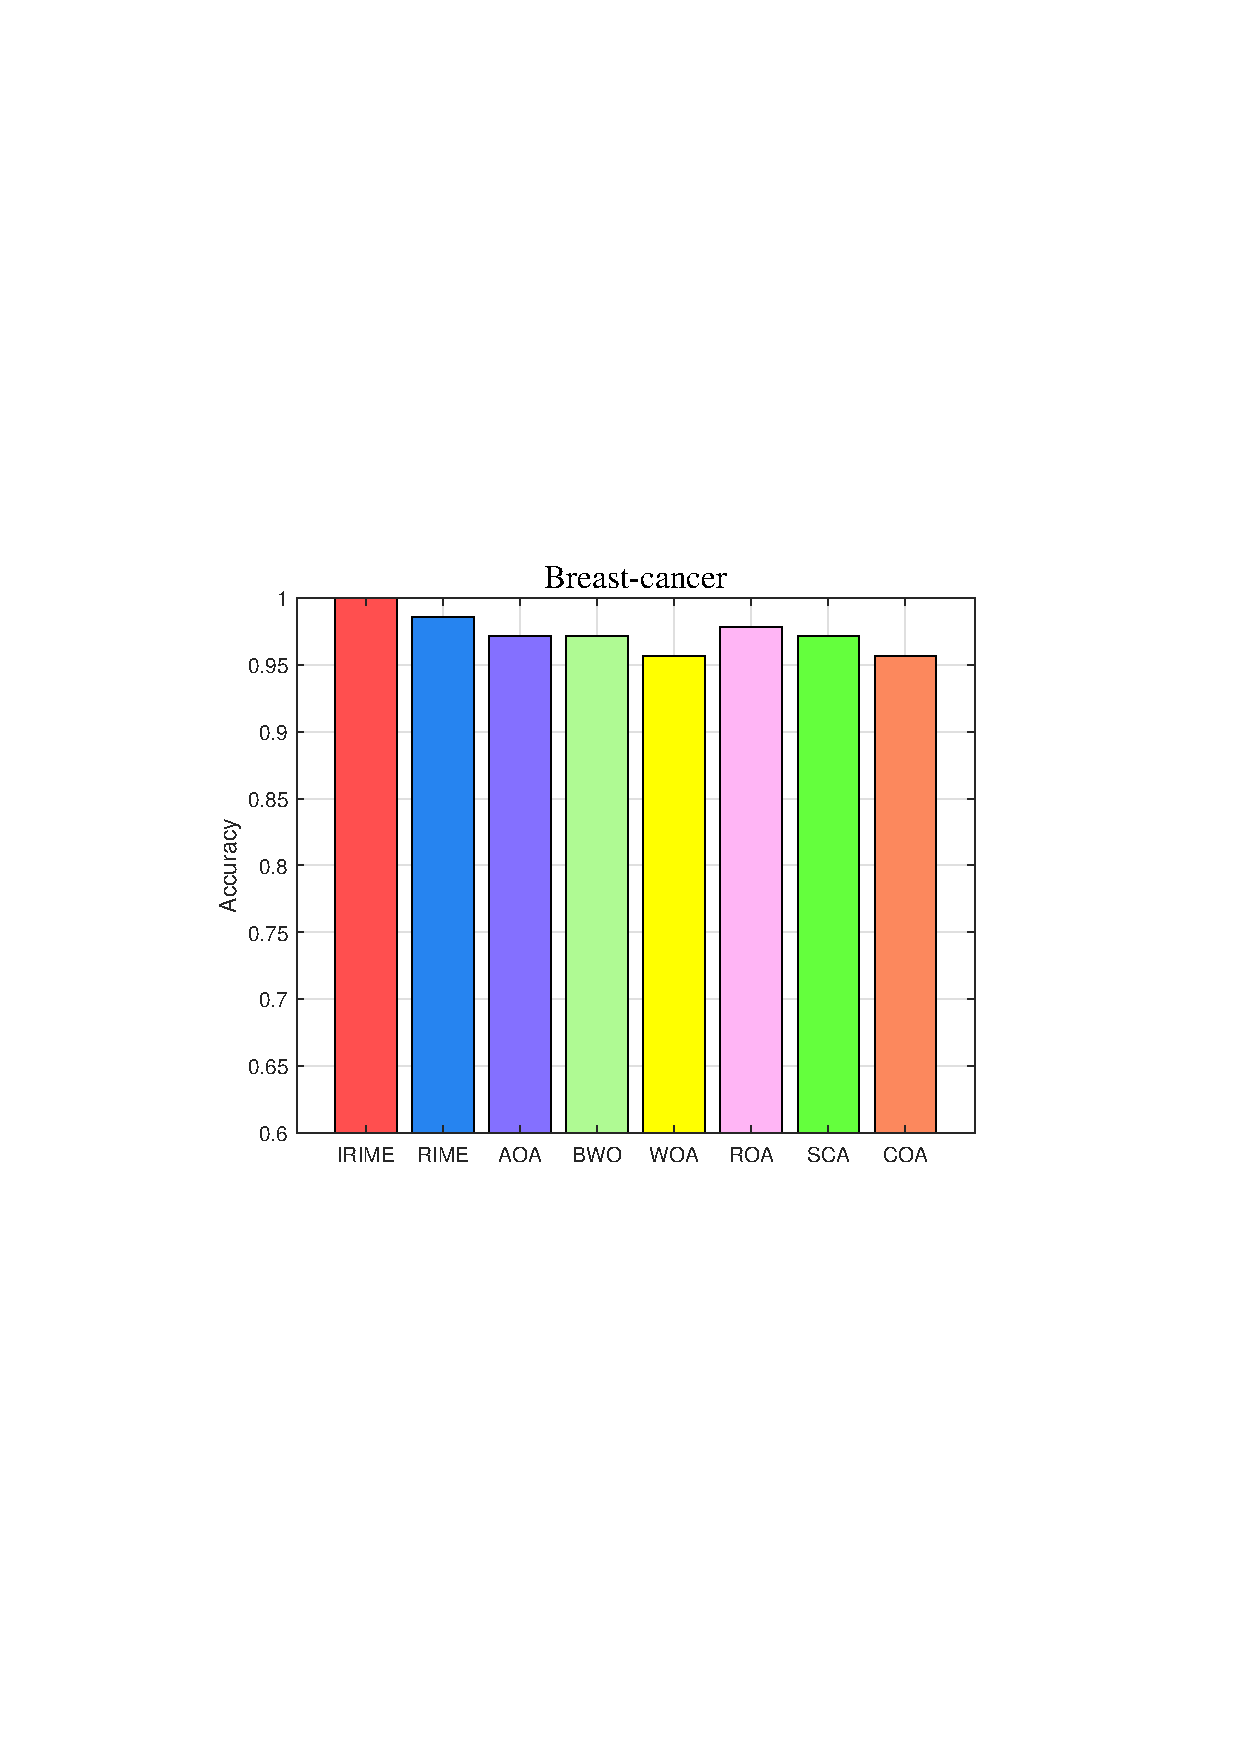
\includegraphics[width=\textwidth]{figures/FS/acc/2.pdf}
    \end{subfigure}
    \hfill
    \begin{subfigure}[b]{0.32\textwidth}
        \caption*{}
        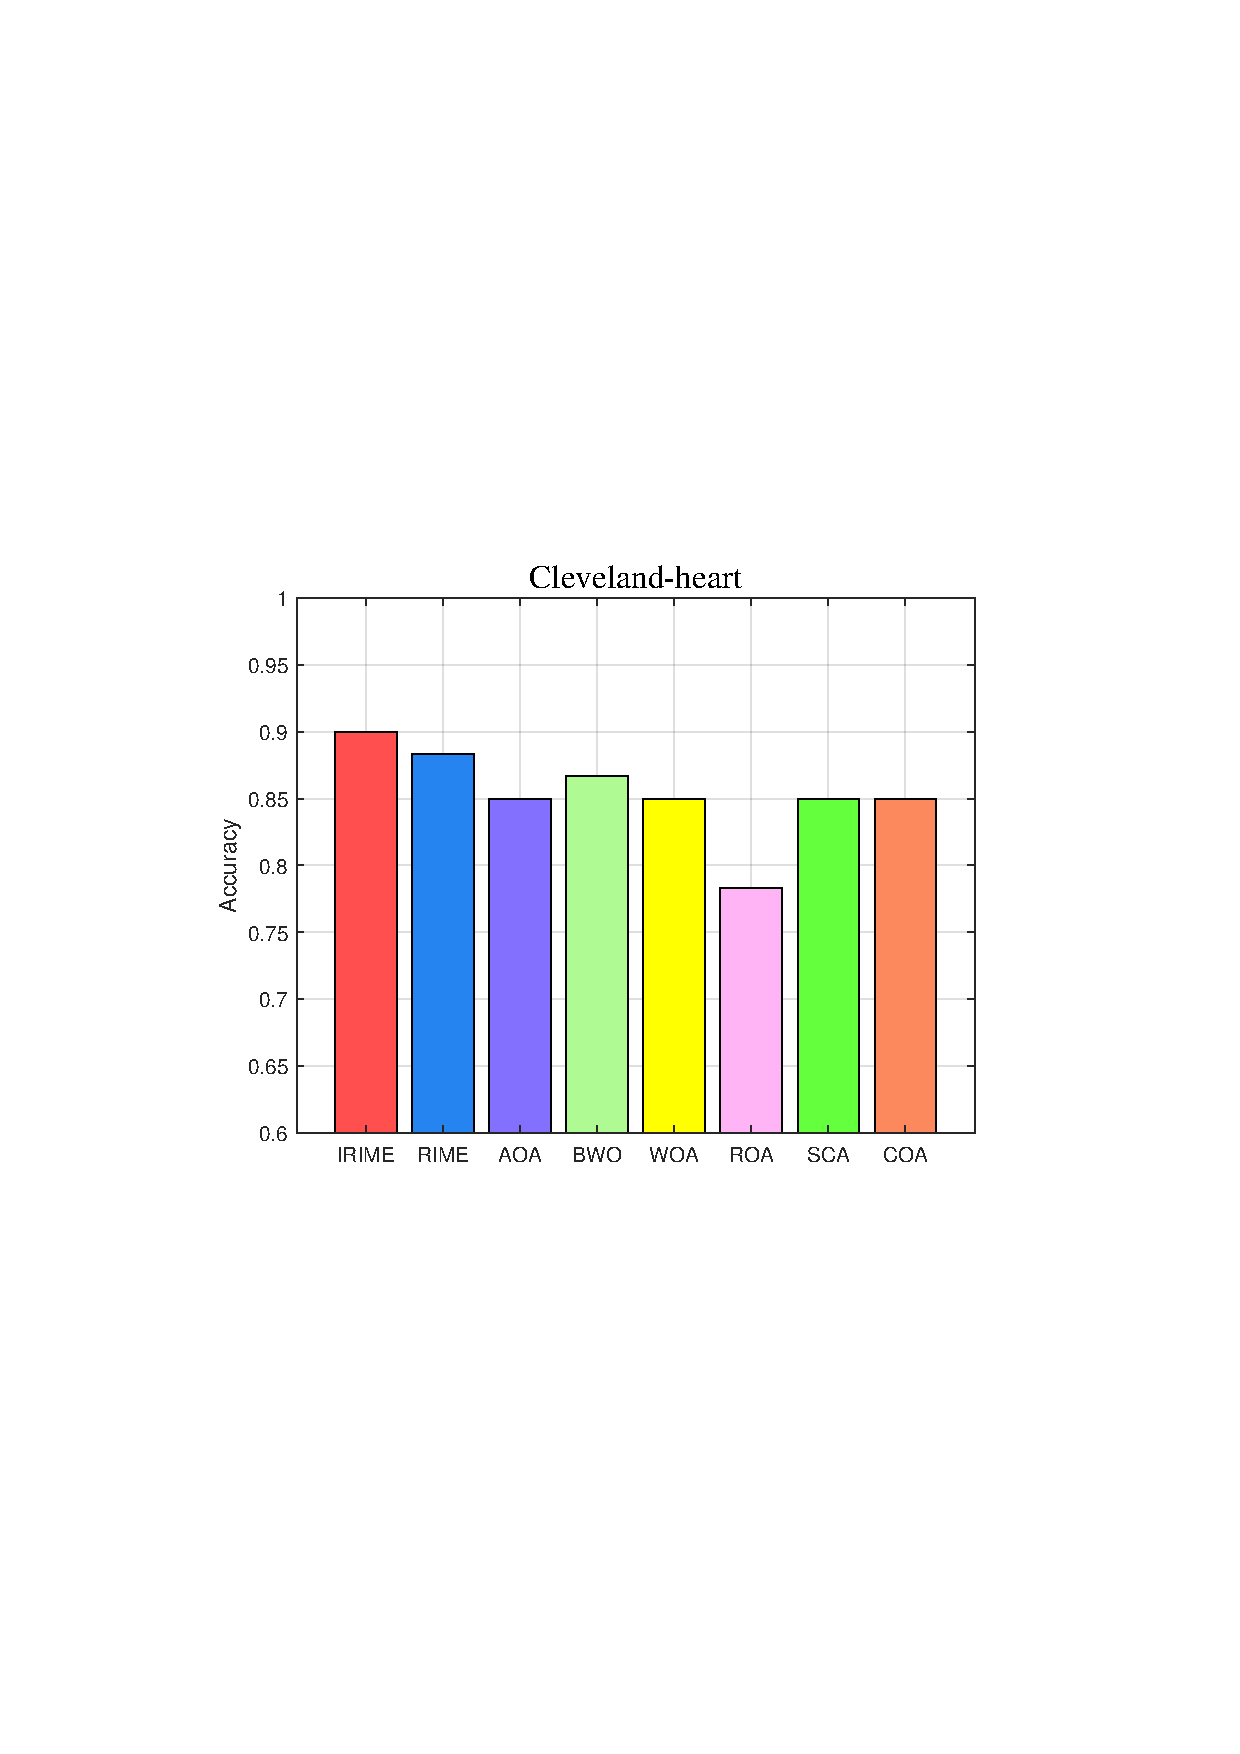
\includegraphics[width=\textwidth]{figures/FS/acc/3.pdf}
    \end{subfigure}
    % 第二行子图
    \begin{subfigure}[b]{0.32\textwidth}
        \caption*{}
        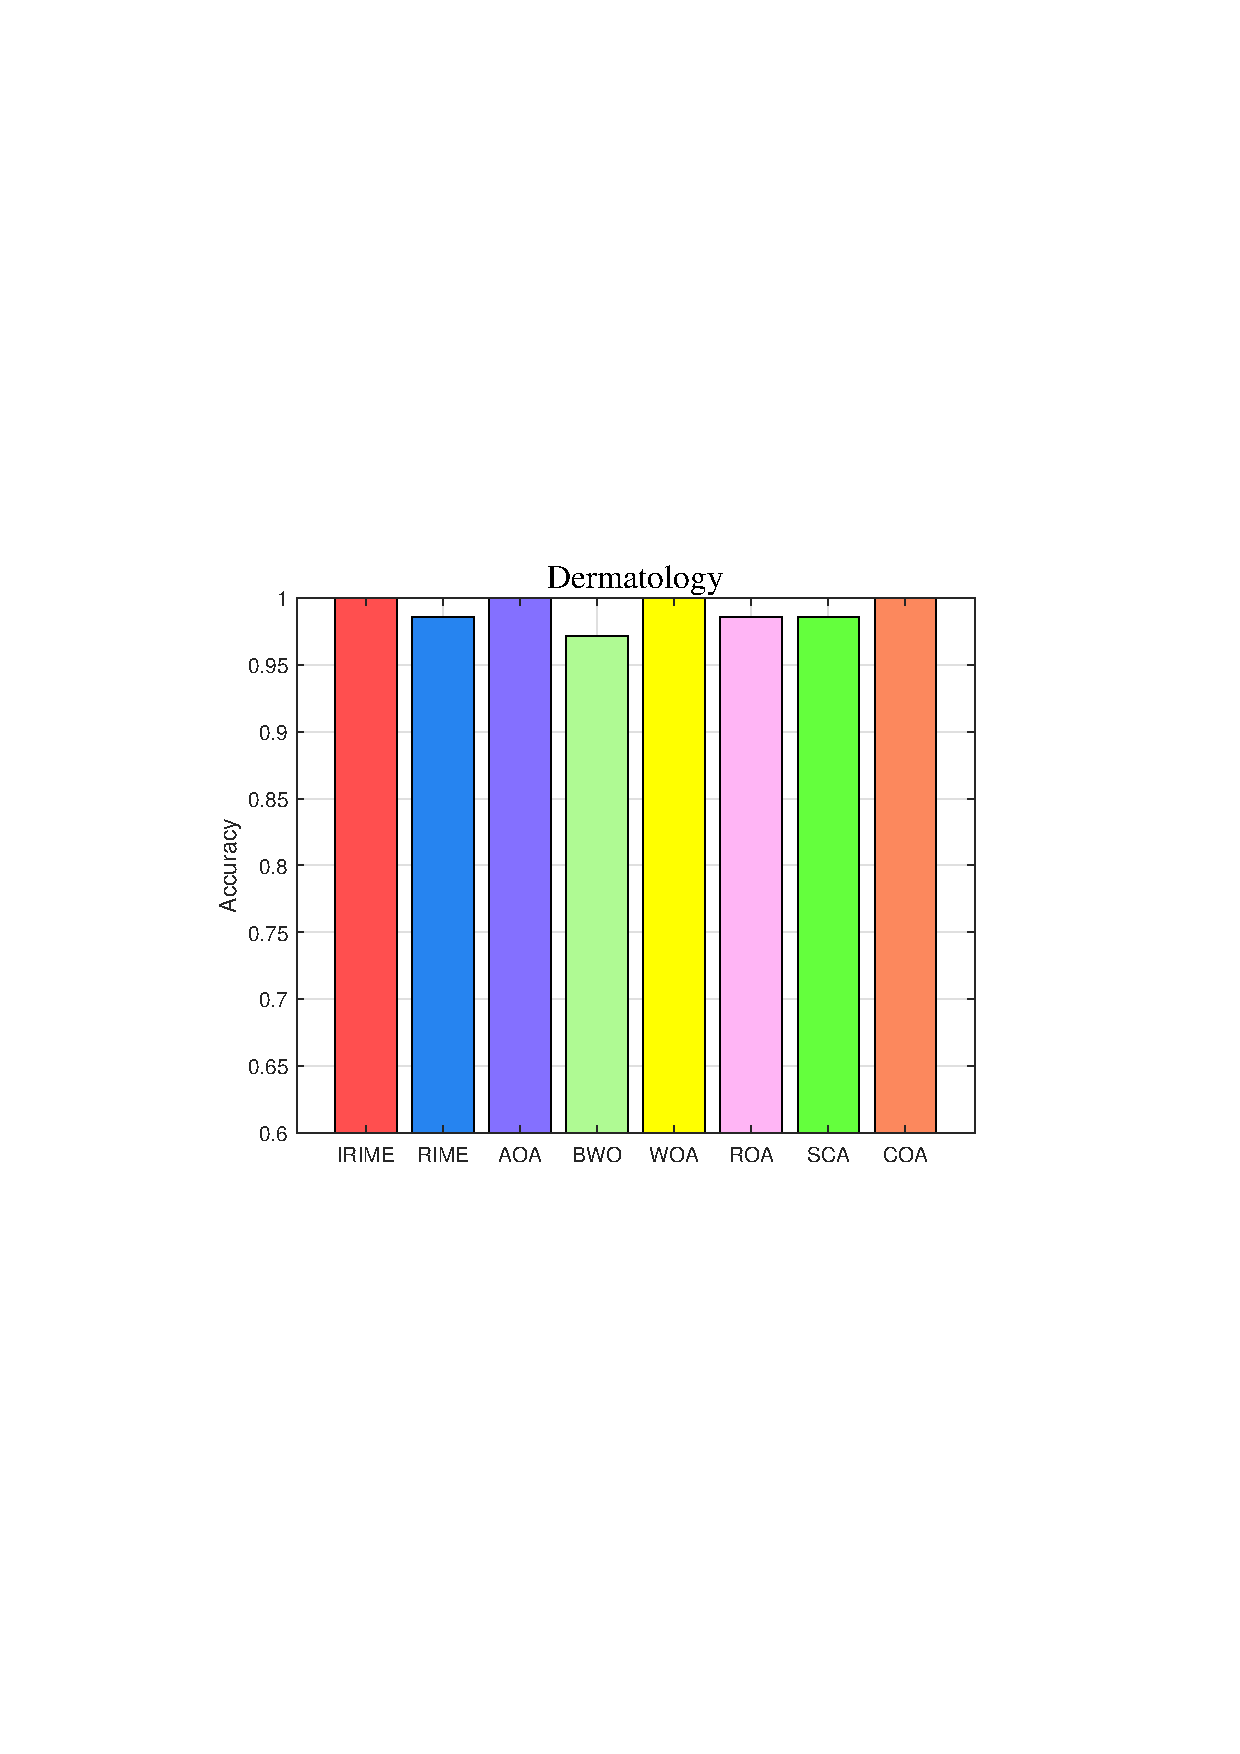
\includegraphics[width=\textwidth]{figures/FS/acc/4.pdf}
    \end{subfigure}
    \hfill
    \begin{subfigure}[b]{0.32\textwidth}
        \caption*{}
        
\includegraphics[width=\textwidth]{figures/FS/acc/5.pdf}
    \end{subfigure}
    \hfill
    \begin{subfigure}[b]{0.32\textwidth}
        \caption*{}
        
\includegraphics[width=\textwidth]{figures/FS/acc/6.pdf}
    \end{subfigure}
    % 第三行子图
    \begin{subfigure}[b]{0.32\textwidth}
        \caption*{}
        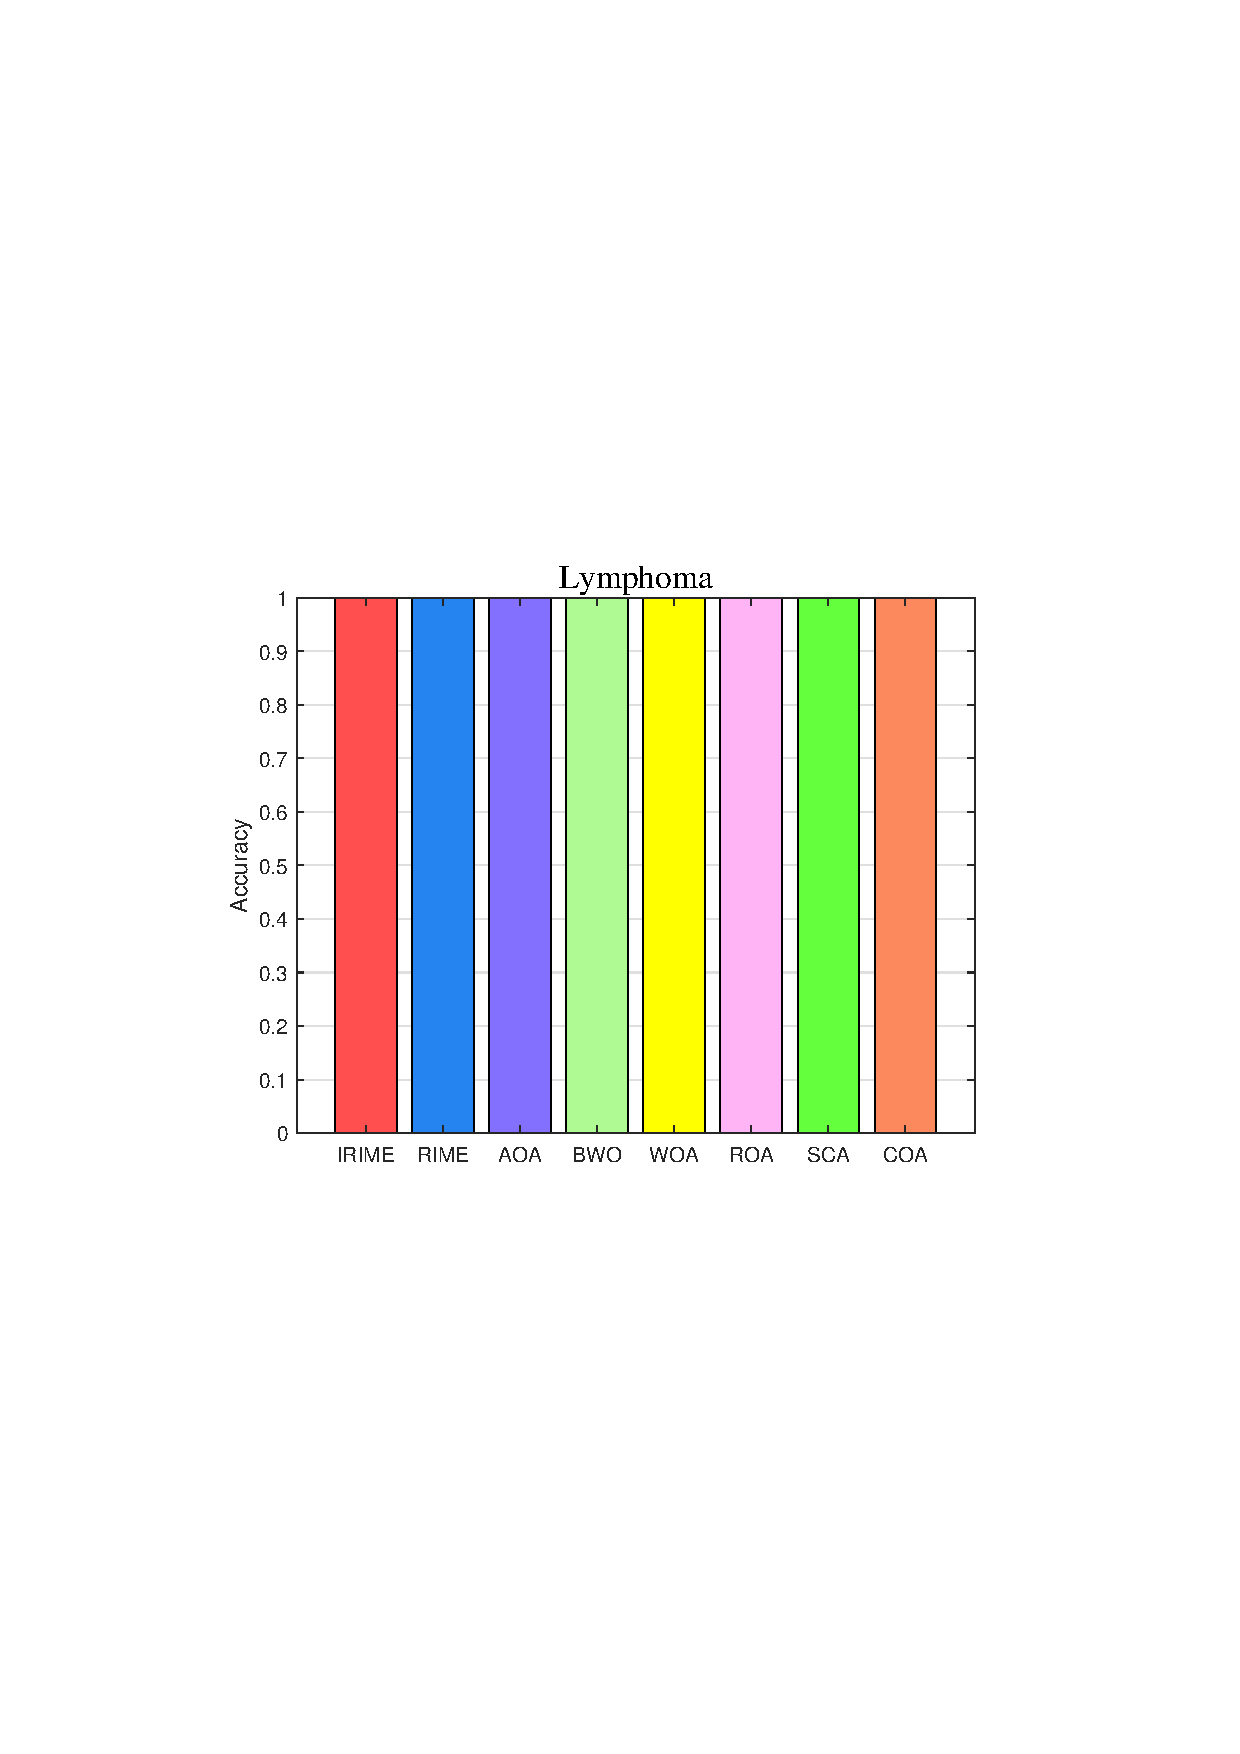
\includegraphics[width=\textwidth]{figures/FS/acc/7.pdf}
    \end{subfigure}
    \hfill
    \begin{subfigure}[b]{0.32\textwidth}
        \caption*{}
        
\includegraphics[width=\textwidth]{figures/FS/acc/8.pdf}
    \end{subfigure}
    \hfill
    \begin{subfigure}[b]{0.32\textwidth}
        \caption*{}
        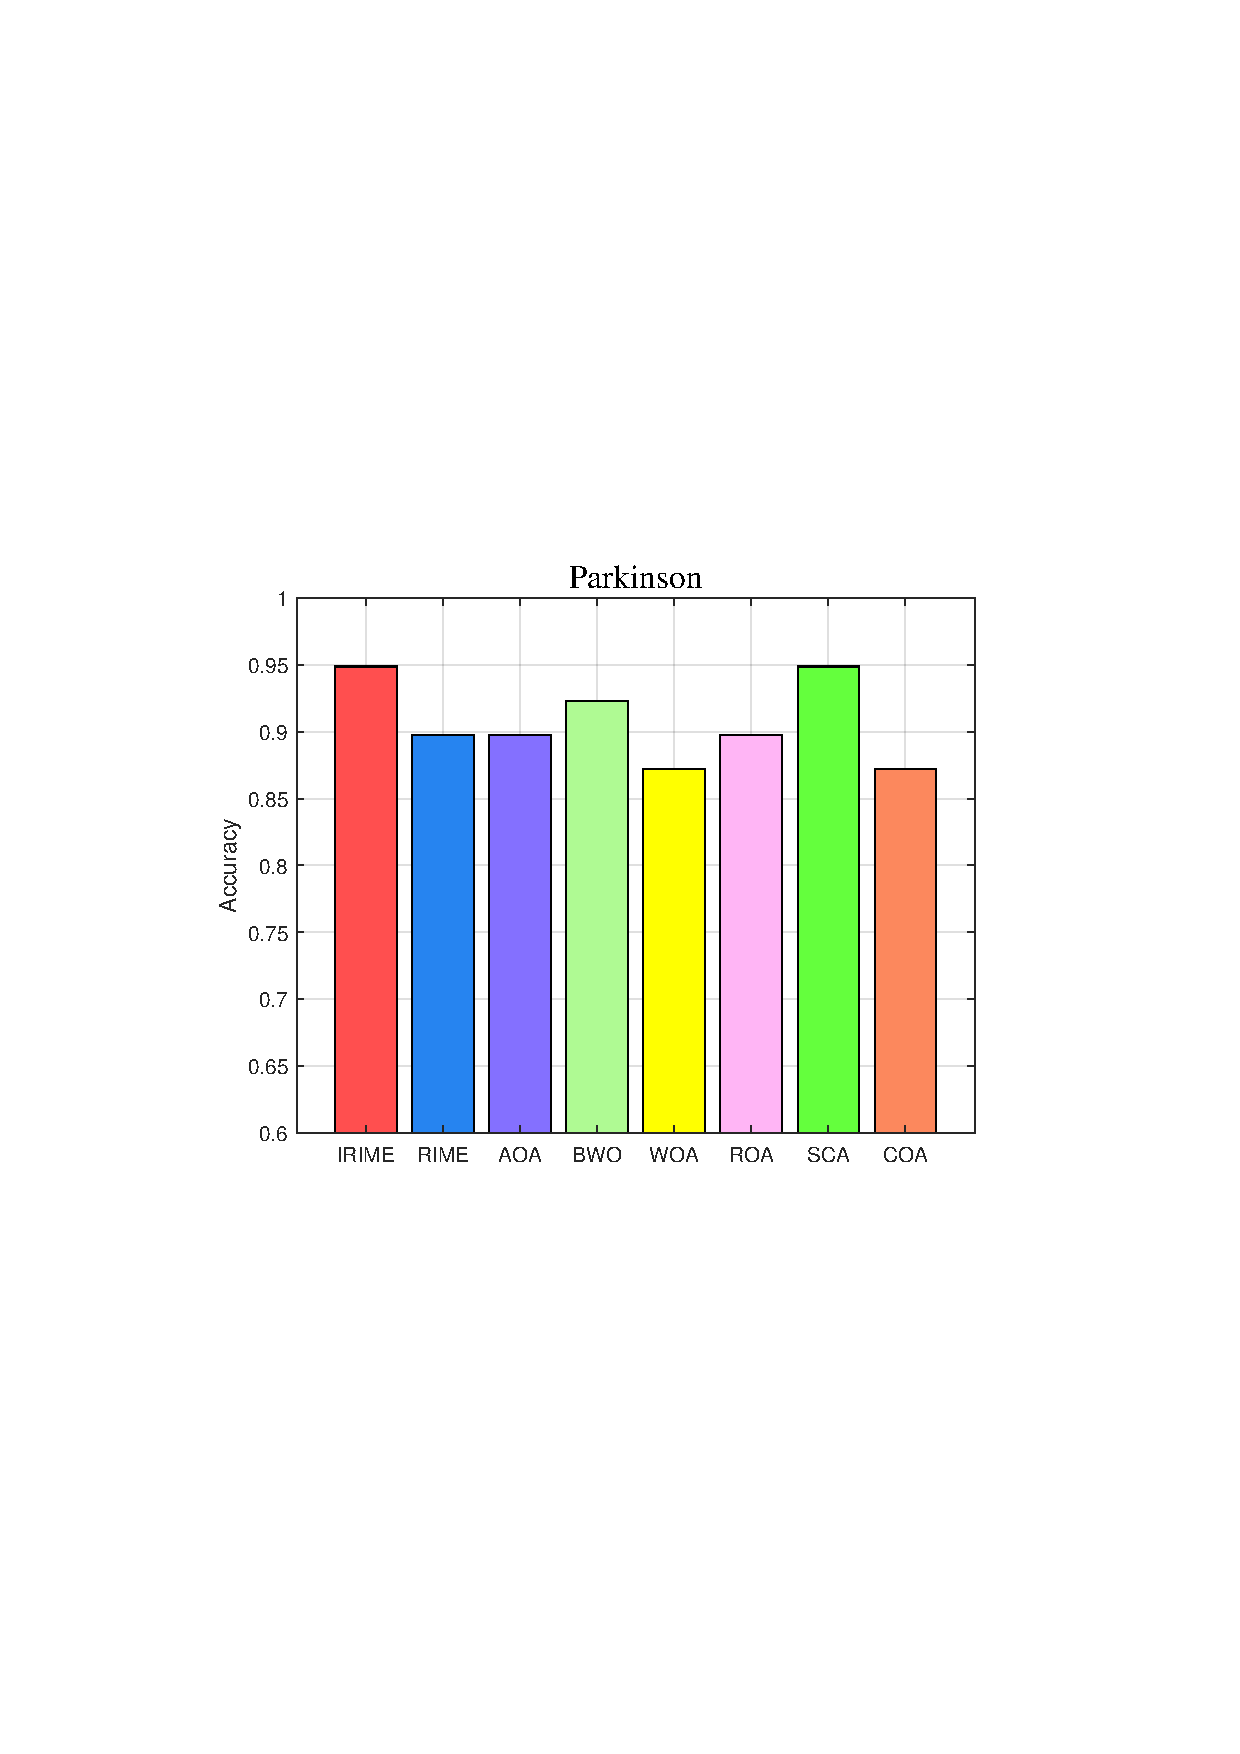
\includegraphics[width=\textwidth]{figures/FS/acc/9.pdf}
    \end{subfigure}
    % 第四行
    \begin{subfigure}[b]{0.32\textwidth}
        \caption*{}
        
\includegraphics[width=\textwidth]{figures/FS/acc/10.pdf}
    \end{subfigure}
    \hfill
    \begin{subfigure}[b]{0.32\textwidth}
        \caption*{}
        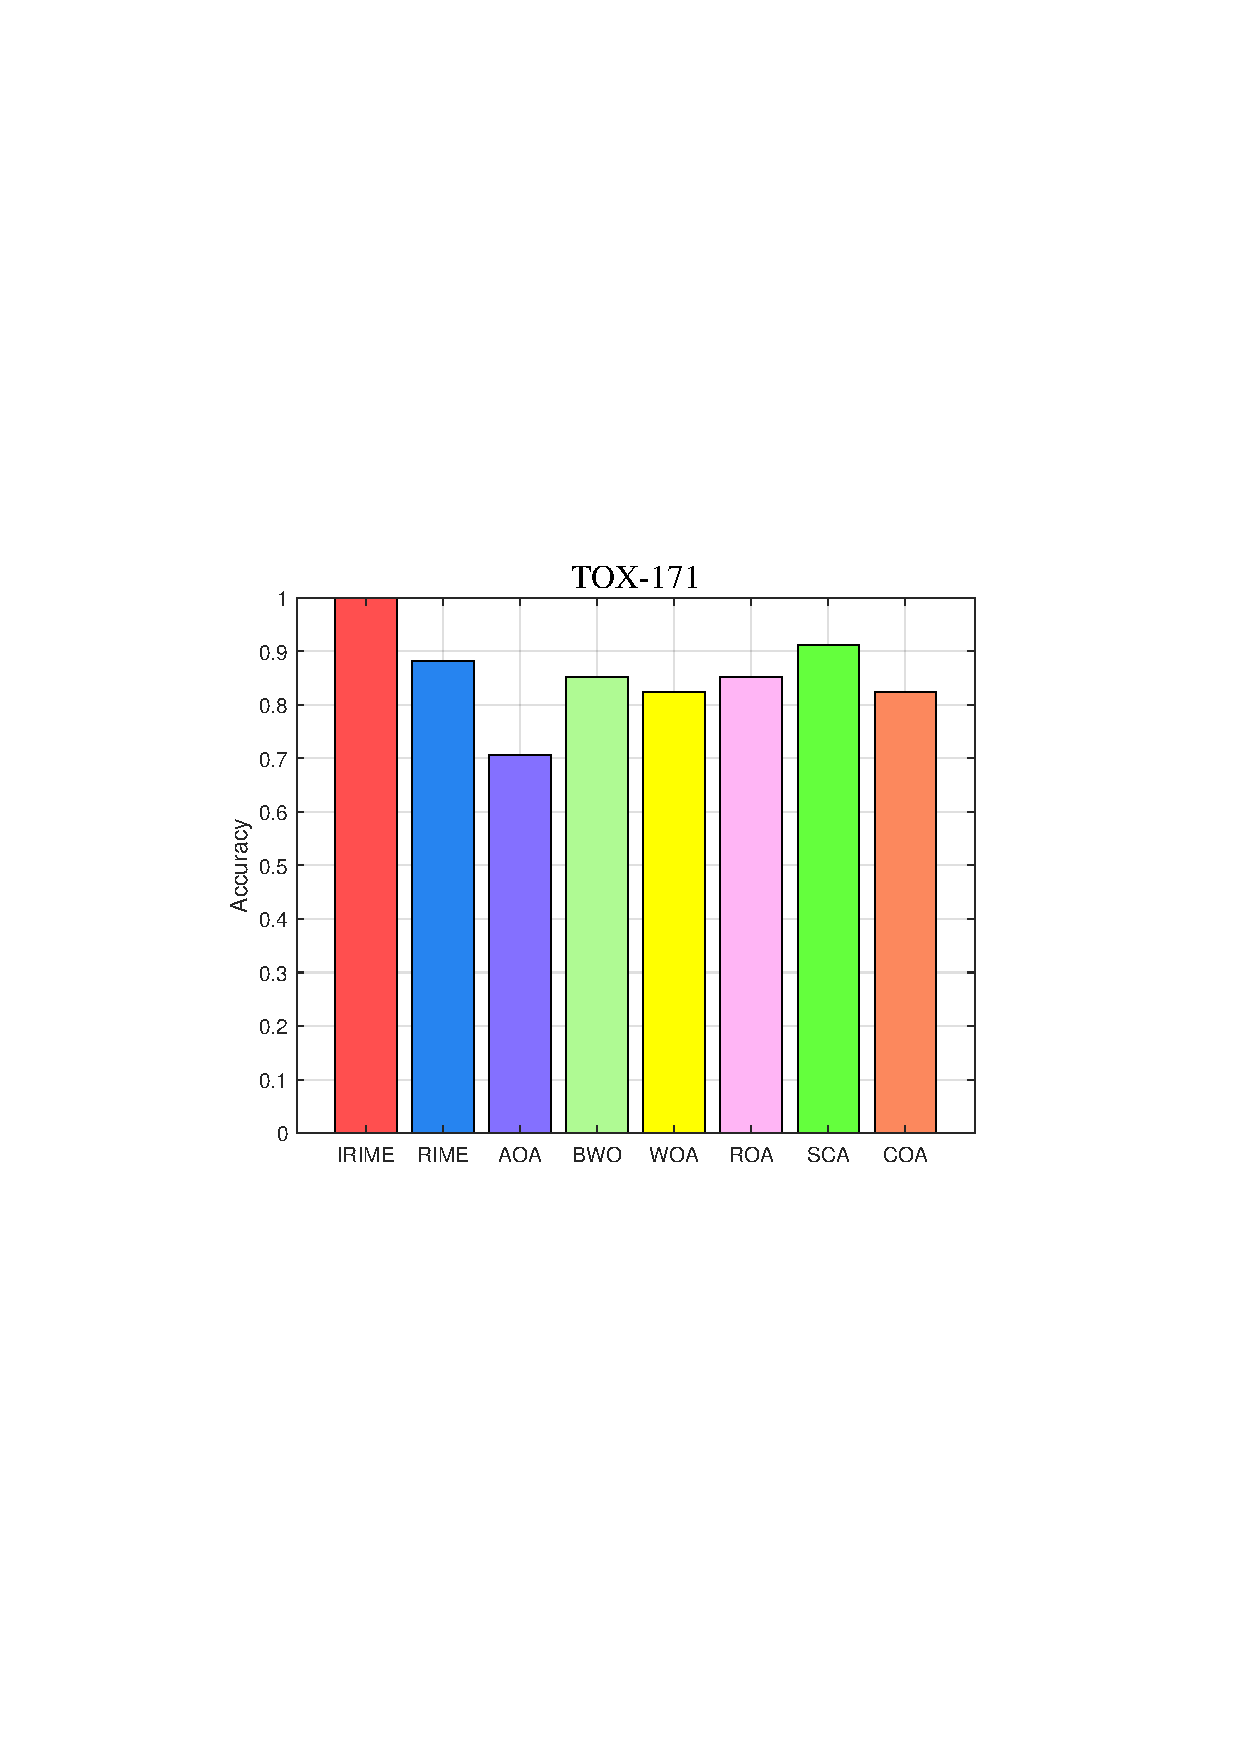
\includegraphics[width=\textwidth]{figures/FS/acc/11.pdf}
    \end{subfigure}
    \hfill
    \begin{subfigure}[b]{0.32\textwidth}
        \caption*{}
        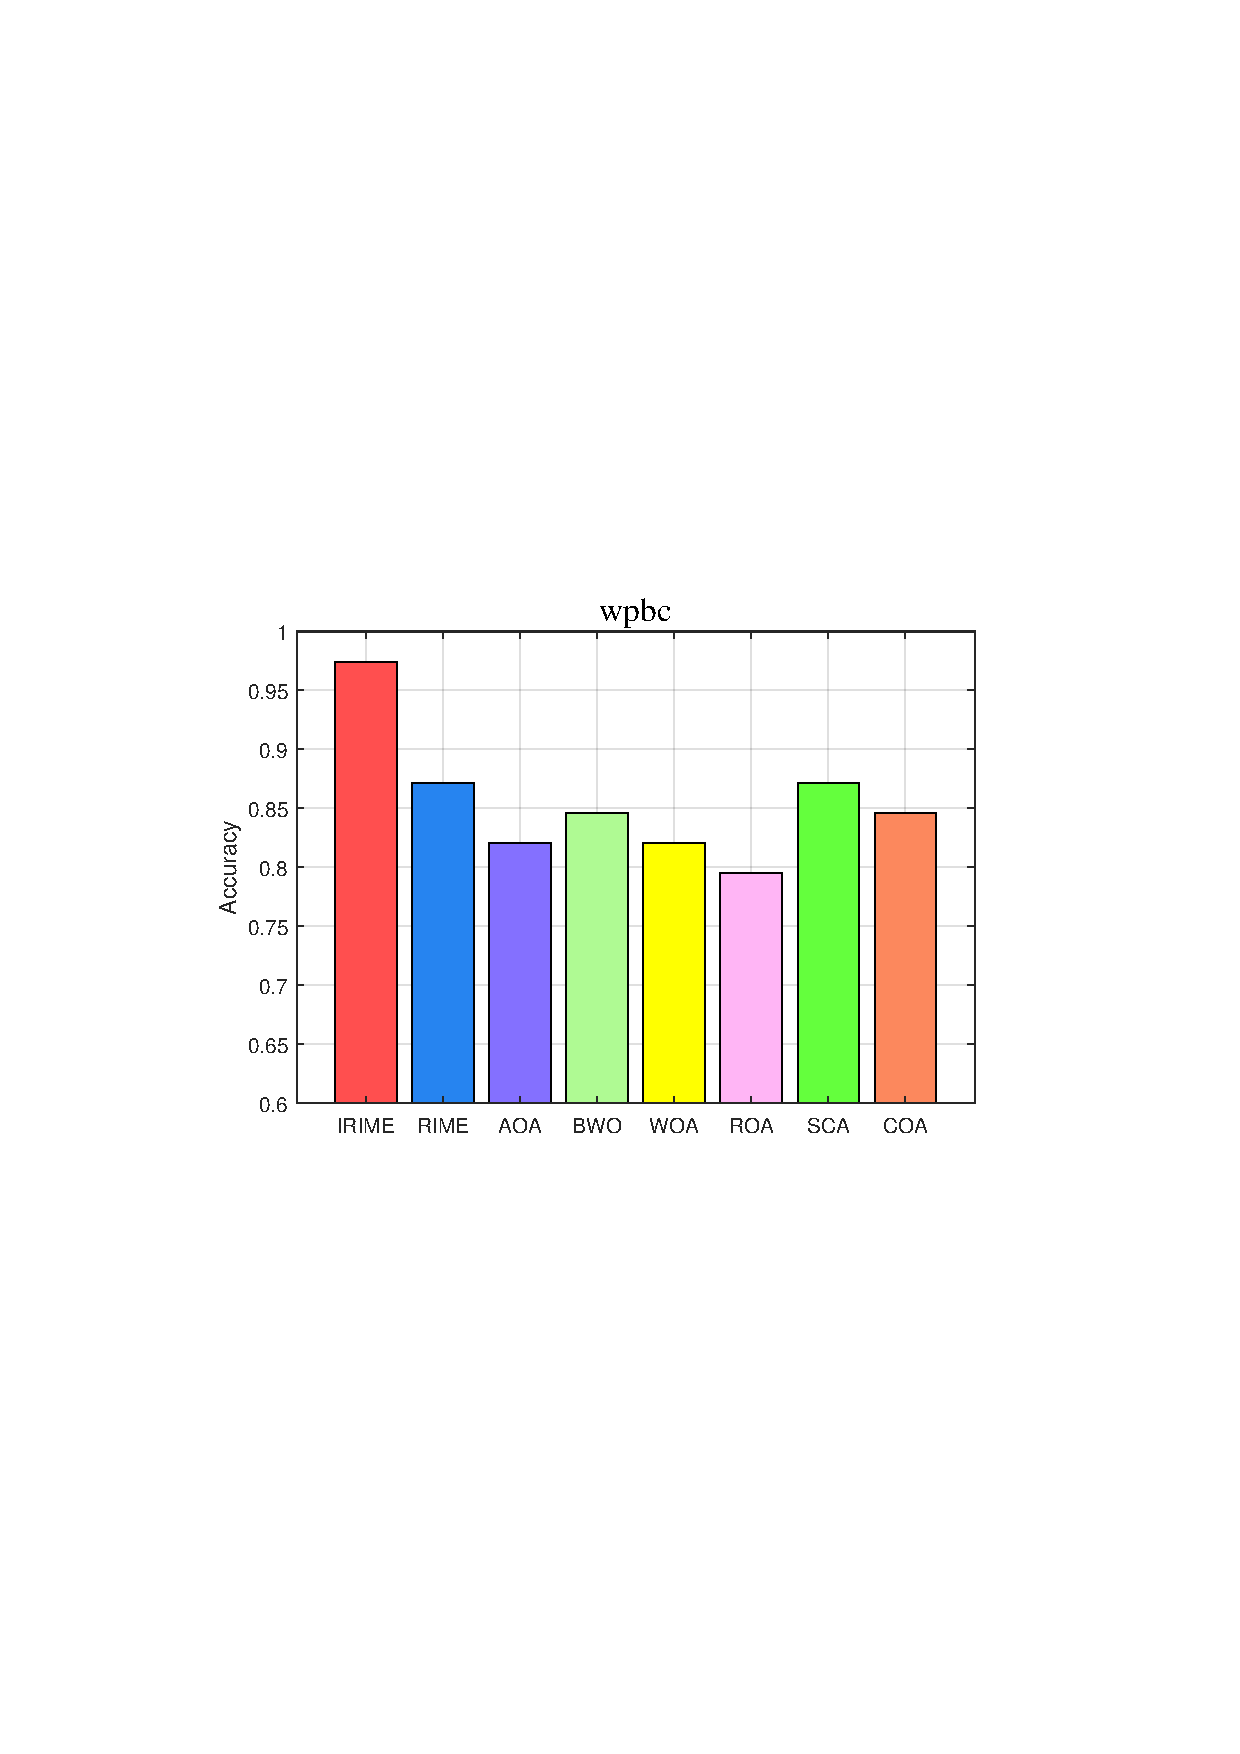
\includegraphics[width=\textwidth]{figures/FS/acc/12.pdf}
    \end{subfigure}
    \caption{12 个数据集上的对比准确率直方图}
    \label{fig:fs-acc}
\end{figure}

\begin{table}[htbp]
  \centering
  \caption{12 个数据集上的适应度值结果}
    \setlength{\tabcolsep}{3pt} % 减少列间距
    \tiny
    \begin{tabular}{cccccccccc}
    \toprule    
    Dataset & Metric & IRIME & RIME  & AOA   & BWO   & WOA   & ROA   & SCA   & COA \\
    \midrule
    \multirow{3}[0]{*}{Breast-cancer} & best  & 4.4444E-03 & 1.7578E-02 & 1.4900E-02 & 3.3333E-03 & 4.4444E-03 & 3.3333E-03 & 1.1567E-02 & 3.3333E-03 \\
          & mean  & 1.9624E-02 & 2.3028E-02 & 2.6478E-02 & 2.0336E-02 & 1.9689E-02 & 2.5877E-02 & 2.5432E-02 & 2.1159E-02 \\
          & std   & 1.1108E-02 & 5.5461E-03 & 1.1300E-02 & 1.1041E-02 & 1.1334E-02 & 1.0368E-02 & 1.1200E-02 & 1.2029E-02 \\
    \multirow{3}[0]{*}{Cleveland-heart} & best  & 6.9846E-02 & 6.9846E-02 & 8.7115E-02 & 5.3346E-02 & 8.8654E-02 & 3.8385E-02 & 6.9846E-02 & 5.5654E-02 \\
          & mean  & 1.0826E-01 & 1.1486E-01 & 1.2253E-01 & 1.2161E-01 & 1.2223E-01 & 1.0903E-01 & 1.1401E-01 & 1.1509E-01 \\
          & std   & 1.9192E-02 & 3.6574E-02 & 3.3669E-02 & 3.3271E-02 & 2.3424E-02 & 4.4835E-02 & 3.0825E-02 & 3.3782E-02 \\
    \multirow{3}[0]{*}{Dermatology} & best  & 1.7647E-03 & 2.3529E-03 & 4.1176E-03 & 5.0000E-03 & 3.8235E-03 & 3.8235E-03 & 1.4706E-03 & 3.2353E-03 \\
          & mean  & 4.2767E-03 & 7.3007E-03 & 1.3031E-02 & 1.5643E-02 & 1.1589E-02 & 1.4807E-02 & 1.1043E-02 & 6.6417E-03 \\
          & std   & 4.3719E-03 & 6.5224E-03 & 1.0056E-02 & 1.2877E-02 & 6.9351E-03 & 7.6337E-03 & 7.2608E-03 & 5.7978E-03 \\
    \multirow{3}[0]{*}{Diabetes} & best  & 1.6676E-01 & 1.7574E-01 & 1.6404E-01 & 1.8743E-01 & 1.8618E-01 & 2.0037E-01 & 1.9140E-01 & 2.0162E-01 \\
          & mean  & 2.0427E-01 & 2.1890E-01 & 2.2082E-01 & 2.1164E-01 & 2.1644E-01 & 2.3310E-01 & 2.1957E-01 & 2.1669E-01 \\
          & std   & 1.9885E-02 & 2.0106E-02 & 2.8935E-02 & 1.9926E-02 & 2.3074E-02 & 2.6184E-02 & 2.1388E-02 & 1.0460E-02 \\
    \multirow{3}[0]{*}{lungcancer-3class} & best  & 3.5714E-04 & 7.1429E-04 & 4.4643E-03 & 1.2500E-03 & 5.3571E-04 & 8.9286E-04 & 3.5714E-04 & 2.3214E-03 \\
          & mean  & 1.7214E-02 & 3.3964E-02 & 1.0418E-01 & 8.4339E-02 & 8.3839E-02 & 1.5043E-01 & 8.3143E-02 & 3.6054E-02 \\
          & std   & 5.2117E-02 & 6.9439E-02 & 1.3867E-01 & 1.1565E-01 & 1.1644E-01 & 1.2116E-01 & 8.7001E-02 & 6.9281E-02 \\
    \multirow{3}[0]{*}{Parkinson} & best  & 9.0909E-04 & 9.0909E-04 & 2.7657E-02 & 3.1818E-03 & 2.6748E-02 & 2.9476E-02 & 1.8182E-03 & 2.2727E-03 \\
          & mean  & 4.6692E-02 & 7.4570E-02 & 5.9892E-02 & 4.2115E-02 & 6.9902E-02 & 8.5678E-02 & 5.9703E-02 & 7.0266E-02 \\
          & std   & 2.6093E-02 & 4.8458E-02 & 3.3682E-02 & 2.0709E-02 & 2.7134E-02 & 3.5320E-02 & 3.1505E-02 & 3.7616E-02 \\
    \multirow{3}[0]{*}{SPECT} & best  & 7.8353E-02 & 5.9220E-02 & 9.9760E-02 & 6.2856E-02 & 8.3353E-02 & 7.9717E-02 & 7.7444E-02 & 4.3268E-02 \\
          & mean  & 1.0815E-01 & 1.1913E-01 & 1.2637E-01 & 1.4036E-01 & 1.2318E-01 & 1.2086E-01 & 1.1548E-01 & 1.0737E-01 \\
          & std   & 2.1731E-02 & 3.3873E-02 & 3.0181E-02 & 4.0193E-02 & 2.7183E-02 & 2.9275E-02 & 2.5141E-02 & 3.8726E-02 \\
    \multirow{3}[0]{*}{wpbc} & best  & 2.7506E-02 & 7.7972E-02 & 1.0730E-01 & 8.1608E-02 & 7.7366E-02 & 1.0366E-01 & 7.7063E-02 & 5.5315E-02 \\
          & mean  & 8.8429E-02 & 1.1161E-01 & 1.4347E-01 & 1.2696E-01 & 1.4672E-01 & 1.4056E-01 & 1.1064E-01 & 1.1811E-01 \\
          & std   & 3.6329E-02 & 2.3809E-02 & 3.3643E-02 & 2.4154E-02 & 3.1608E-02 & 2.6510E-02 & 2.4200E-02 & 5.0897E-02 \\
    \multirow{3}[0]{*}{ALLAML} & best  & 1.4027E-06 & 8.4163E-06 & 7.5650E-02 & 2.8054E-06 & 1.4027E-06 & 2.8054E-06 & 7.1539E-05 & 7.5319E-02 \\
          & mean  & 3.6471E-06 & 1.4210E-02 & 1.5397E-01 & 2.1221E-02 & 2.8295E-02 & 7.7909E-02 & 1.4248E-02 & 1.3198E-01 \\
          & std   & 1.5079E-06 & 2.9868E-02 & 5.2247E-02 & 3.4156E-02 & 3.6511E-02 & 7.0353E-02 & 2.9826E-02 & 6.4967E-02 \\
    \multirow{3}[0]{*}{Lymphoma} & best  & 2.4839E-06 & 4.9677E-06 & 4.7889E-03 & 2.4839E-06 & 4.9677E-06 & 7.4516E-06 & 7.4516E-06 & 7.6006E-04 \\
          & mean  & 4.7193E-06 & 7.2032E-06 & 4.8530E-03 & 2.9806E-06 & 8.9419E-06 & 1.7139E-05 & 1.5152E-05 & 4.1381E-03 \\
          & std   & 1.4100E-06 & 2.1749E-06 & 5.3077E-05 & 1.0473E-06 & 3.9186E-06 & 1.4024E-05 & 9.0281E-06 & 1.1887E-03 \\
    \multirow{3}[0]{*}{nci9} & best  & 1.6501E-01 & 2.4767E-01 & 4.1957E-01 & 2.4751E-01 & 2.4753E-01 & 3.3009E-01 & 2.4761E-01 & 4.1726E-01 \\
          & mean  & 2.7228E-01 & 3.4662E-01 & 5.5840E-01 & 3.6318E-01 & 3.6310E-01 & 4.5414E-01 & 3.4668E-01 & 5.5754E-01 \\
          & std   & 1.1034E-01 & 7.5740E-02 & 8.6980E-02 & 9.6622E-02 & 8.8655E-02 & 7.9960E-02 & 6.5048E-02 & 1.2324E-01 \\
    \multirow{3}[0]{*}{TOX-171} & best  & 1.6875E-04 & 3.2026E-02 & 1.5065E-01 & 8.7480E-02 & 3.1633E-02 & 6.4942E-02 & 2.9420E-02 & 6.3251E-02 \\
          & mean  & 3.5686E-02 & 9.5800E-02 & 2.2457E-01 & 1.5284E-01 & 1.3361E-01 & 1.5890E-01 & 7.6619E-02 & 1.3883E-01 \\
          & std   & 3.8437E-02 & 4.2697E-02 & 6.4879E-02 & 4.9116E-02 & 5.6303E-02 & 4.6560E-02 & 2.8391E-02 & 3.9287E-02 \\
    \bottomrule      
    \end{tabular}%
  \label{tb:FS-fitness}%
\end{table}%

\begin{table}[htbp]
  \centering
  \caption{12 个数据集上的准确率结果}
    \setlength{\tabcolsep}{3pt} % 减少列间距
    \tiny
    \begin{tabular}{cccccccccc}
    \toprule    
    Dataset & Metric & IRIME & RIME  & AOA   & BWO   & WOA   & ROA   & SCA   & COA \\
    \midrule
    \multirow{3}[0]{*}{Breast-cancer} & best  & 9.6403E-01 & 9.7122E-01 & 9.4964E-01 & 9.6403E-01 & 9.6403E-01 & 9.6403E-01 & 9.5683E-01 & 9.6403E-01 \\
          & mean  & 9.8489E-01 & 9.8201E-01 & 9.7842E-01 & 9.8417E-01 & 9.8561E-01 & 9.7914E-01 & 9.7914E-01 & 9.8345E-01 \\
          & std   & 1.0963E-02 & 5.0871E-03 & 1.2228E-02 & 1.0617E-02 & 1.1248E-02 & 9.8584E-03 & 1.1476E-02 & 1.1773E-02 \\
    \multirow{3}[0]{*}{Cleveland-heart} & best  & 8.6667E-01 & 8.1667E-01 & 8.3333E-01 & 8.3333E-01 & 8.5000E-01 & 8.5000E-01 & 8.1667E-01 & 8.5000E-01 \\
          & mean  & 8.9500E-01 & 8.8833E-01 & 8.8167E-01 & 8.8167E-01 & 8.8167E-01 & 8.9500E-01 & 8.8833E-01 & 8.8833E-01 \\
          & std   & 1.9325E-02 & 3.6893E-02 & 3.4650E-02 & 3.3747E-02 & 2.4152E-02 & 4.5168E-02 & 3.1476E-02 & 3.4292E-02 \\
    \multirow{3}[0]{*}{Dermatology} & best  & 9.8592E-01 & 9.8592E-01 & 9.7183E-01 & 9.5775E-01 & 9.8592E-01 & 9.8592E-01 & 9.8592E-01 & 9.8592E-01 \\
          & mean  & 9.9859E-01 & 9.9577E-01 & 9.9296E-01 & 9.9014E-01 & 9.9296E-01 & 9.9155E-01 & 9.9155E-01 & 9.9718E-01 \\
          & std   & 4.4539E-03 & 6.8035E-03 & 9.9593E-03 & 1.3362E-02 & 7.4232E-03 & 7.2732E-03 & 7.2732E-03 & 5.9385E-03 \\
    \multirow{3}[0]{*}{Diabetes} & best  & 7.5817E-01 & 7.5817E-01 & 7.4510E-01 & 7.5163E-01 & 7.5163E-01 & 7.5163E-01 & 7.4510E-01 & 7.7124E-01 \\
          & mean  & 7.8824E-01 & 7.8431E-01 & 7.8301E-01 & 7.9216E-01 & 7.8693E-01 & 7.8497E-01 & 7.8301E-01 & 7.8693E-01 \\
          & std   & 1.8538E-02 & 2.0897E-02 & 3.0314E-02 & 2.0391E-02 & 2.1830E-02 & 2.3756E-02 & 2.1743E-02 & 1.1610E-02 \\
    \multirow{3}[0]{*}{lungcancer-3class} & best  & 8.3333E-01 & 1.0000E+00 & 6.6667E-01 & 6.6667E-01 & 6.6667E-01 & 6.6667E-01 & 8.3333E-01 & 8.3333E-01 \\
          & mean  & 9.8333E-01 & 1.0000E+00 & 9.0000E-01 & 9.1667E-01 & 9.1667E-01 & 8.5000E-01 & 9.1667E-01 & 9.6667E-01 \\
          & std   & 5.2705E-02 & 0.0000E+00 & 1.4055E-01 & 1.1785E-01 & 1.1785E-01 & 1.2298E-01 & 8.7841E-02 & 7.0273E-02 \\
    \multirow{3}[0]{*}{Parkinson} & best  & 9.2308E-01 & 8.4615E-01 & 8.9744E-01 & 9.2308E-01 & 8.9744E-01 & 8.4615E-01 & 8.9744E-01 & 8.7179E-01 \\
          & mean  & 9.5385E-01 & 9.2564E-01 & 9.4359E-01 & 9.5897E-01 & 9.3077E-01 & 9.1538E-01 & 9.4103E-01 & 9.3077E-01 \\
          & std   & 2.6482E-02 & 4.9024E-02 & 3.3758E-02 & 2.1622E-02 & 2.7163E-02 & 3.6362E-02 & 3.2094E-02 & 3.8319E-02 \\
    \multirow{3}[0]{*}{SPECT} & best  & 8.6792E-01 & 8.1132E-01 & 8.3019E-01 & 7.9245E-01 & 8.3019E-01 & 8.3019E-01 & 8.4906E-01 & 8.3019E-01 \\
          & mean  & 8.9434E-01 & 8.8302E-01 & 8.7925E-01 & 8.6226E-01 & 8.8113E-01 & 8.8302E-01 & 8.8679E-01 & 8.9623E-01 \\
          & std   & 2.2147E-02 & 3.4218E-02 & 3.1067E-02 & 4.1766E-02 & 2.8197E-02 & 2.9230E-02 & 2.5157E-02 & 4.0025E-02 \\
    \multirow{3}[0]{*}{wpbc} & best  & 8.7179E-01 & 8.4615E-01 & 7.9487E-01 & 8.4615E-01 & 8.2051E-01 & 8.2051E-01 & 8.7179E-01 & 7.9487E-01 \\
          & mean  & 9.1282E-01 & 8.8974E-01 & 8.6154E-01 & 8.7436E-01 & 8.5385E-01 & 8.6154E-01 & 8.8974E-01 & 8.8462E-01 \\
          & std   & 3.6663E-02 & 2.4325E-02 & 3.4613E-02 & 2.5498E-02 & 3.2094E-02 & 2.7563E-02 & 2.4325E-02 & 5.1637E-02 \\
    \multirow{3}[0]{*}{ALLAML} & best  & 1.0000E+00 & 9.2857E-01 & 7.8571E-01 & 9.2857E-01 & 9.2857E-01 & 7.8571E-01 & 1.0000E+00 & 7.1429E-01 \\
          & mean  & 1.0000E+00 & 9.8571E-01 & 8.5000E-01 & 9.7857E-01 & 9.7143E-01 & 9.2143E-01 & 1.0000E+00 & 8.7143E-01 \\
          & std   & 0.0000E+00 & 3.0117E-02 & 5.2705E-02 & 3.4503E-02 & 3.6886E-02 & 7.1031E-02 & 0.0000E+00 & 6.5638E-02 \\
    \multirow{3}[0]{*}{Lymphoma} & best  & 1.0000E+00 & 1.0000E+00 & 1.0000E+00 & 1.0000E+00 & 1.0000E+00 & 1.0000E+00 & 1.0000E+00 & 1.0000E+00 \\
          & mean  & 1.0000E+00 & 1.0000E+00 & 1.0000E+00 & 1.0000E+00 & 1.0000E+00 & 1.0000E+00 & 1.0000E+00 & 1.0000E+00 \\
          & std   & 0.0000E+00 & 0.0000E+00 & 0.0000E+00 & 0.0000E+00 & 0.0000E+00 & 0.0000E+00 & 0.0000E+00 & 0.0000E+00 \\
    \multirow{3}[0]{*}{nci9} & best  & 5.0000E-01 & 5.0000E-01 & 3.3333E-01 & 5.0000E-01 & 5.0000E-01 & 4.1667E-01 & 5.8333E-01 & 1.6667E-01 \\
          & mean  & 7.2500E-01 & 6.5000E-01 & 4.7500E-01 & 6.3333E-01 & 6.3333E-01 & 5.4167E-01 & 6.5000E-01 & 4.4167E-01 \\
          & std   & 1.1146E-01 & 7.6578E-02 & 9.6625E-02 & 9.7816E-02 & 8.9581E-02 & 8.0985E-02 & 6.5734E-02 & 1.2454E-01 \\
    \multirow{3}[0]{*}{TOX-171} & best  & 8.8235E-01 & 8.8235E-01 & 7.0588E-01 & 7.9412E-01 & 7.9412E-01 & 7.9412E-01 & 8.8235E-01 & 8.2353E-01 \\
          & mean  & 9.6471E-01 & 9.4412E-01 & 8.0294E-01 & 8.4706E-01 & 8.6765E-01 & 8.4412E-01 & 9.2353E-01 & 8.6471E-01 \\
          & std   & 3.8722E-02 & 2.9248E-02 & 6.0515E-02 & 4.9604E-02 & 5.7585E-02 & 4.8129E-02 & 2.8414E-02 & 3.9703E-02 \\
    \bottomrule      
    \end{tabular}%
  \label{tb:FS-acc}%
\end{table}%

%特征选择featureSize图
\begin{figure}[htbp]
    \centering
    % 第一行子图
    \begin{subfigure}[b]{0.32\textwidth}
        \caption*{}
        
\includegraphics[width=\textwidth]{figures/FS/feature/1.pdf}
    \end{subfigure}
    \hfill
    \begin{subfigure}[b]{0.32\textwidth}
        \caption*{}
        
\includegraphics[width=\textwidth]{figures/FS/feature/2.pdf}
    \end{subfigure}
    \hfill
    \begin{subfigure}[b]{0.32\textwidth}
        \caption*{}
        
\includegraphics[width=\textwidth]{figures/FS/feature/3.pdf}
    \end{subfigure}
    % 第二行子图
    \begin{subfigure}[b]{0.32\textwidth}
        \caption*{}
        
\includegraphics[width=\textwidth]{figures/FS/feature/4.pdf}
    \end{subfigure}
    \hfill
    \begin{subfigure}[b]{0.32\textwidth}
        \caption*{}
        
\includegraphics[width=\textwidth]{figures/FS/feature/5.pdf}
    \end{subfigure}
    \hfill
    \begin{subfigure}[b]{0.32\textwidth}
        \caption*{}
        
\includegraphics[width=\textwidth]{figures/FS/feature/6.pdf}
    \end{subfigure}
    % 第三行子图
    \begin{subfigure}[b]{0.32\textwidth}
        \caption*{}
        
\includegraphics[width=\textwidth]{figures/FS/feature/7.pdf}
    \end{subfigure}
    \hfill
    \begin{subfigure}[b]{0.32\textwidth}
        \caption*{}
        
\includegraphics[width=\textwidth]{figures/FS/feature/8.pdf}
    \end{subfigure}
    \hfill
    \begin{subfigure}[b]{0.32\textwidth}
        \caption*{}
        
\includegraphics[width=\textwidth]{figures/FS/feature/9.pdf}
    \end{subfigure}
    % 第四行
    \begin{subfigure}[b]{0.32\textwidth}
        \caption*{}
        
\includegraphics[width=\textwidth]{figures/FS/feature/10.pdf}
    \end{subfigure}
    \hfill
    \begin{subfigure}[b]{0.32\textwidth}
        \caption*{}
        
\includegraphics[width=\textwidth]{figures/FS/feature/11.pdf}
    \end{subfigure}
    \hfill
    \begin{subfigure}[b]{0.32\textwidth}
        \caption*{}
        
\includegraphics[width=\textwidth]{figures/FS/feature/12.pdf}
    \end{subfigure}
    \caption{12 个数据集上的对比特征数量直方图}
    \label{fig:fs-feature}
\end{figure}


在医学特征选择的评估中，IRIME在适应度值和准确率指标方面都表现出显著优势。就适应度值而言，IRIME在多个数据集上始终表现良好。具体而言，在乳腺癌数据集上，其最佳适应度值为0.0044，与WOA并列第二，略高于BWO和ROA。在皮肤科数据集上，IRIME实现了最佳适应度值0.0018，仅次于SCA，且明显优于其他对比算法，彰显其强大的优化能力。在肺癌三分类和wpbc数据集上，IRIME分别取得了0.0003和0.0275的最佳适应度值，在所有比较算法中排名第一。此外，IRIME在不同数据集上的标准差保持适中，例如乳腺癌数据集的标准差为0.0111，表明其具有稳定且高性能的表现。在平均适应度值方面，IRIME在皮肤科数据集上的平均值为0.0043，远低于AOA和BWO，且仅次于SCA。在分类准确率方面，IRIME在多个五个数据集上获得了最高和平均的准确率。例如，在乳腺癌数据集上的最佳准确率与其他领先算法相当，平均准确率达98.49\%，位居前列。这些结果表明，IRIME不仅能有效选择相关特征，还能保持稳健的分类准确性。在高维数据集ALLAML和TOX-171上，IRIME分别以100\%和88.24\%的分类准确率夺得第一，且在其他高维数据集上表现具有竞争力。此外，IRIME在所有高维数据集上的适应度值表现出压倒性的优势。

本节旨在通过选择医学特征选择（FS）问题作为案例，提升IRIME在工程问题中的清晰度和有效性，以评估其优化性能。为确保全面评估，我们将所提方法与七种先进的元启发式算法进行比较：RIME、AOA、BWO、WOA、ROA、SCA和COA。所有算法的参数设置均统一，种群规模为N=30
，每次运行的最大计算预算为3000次迭代，具体详见表8。本研究所用的所有实验数据集均来自医学领域。数据集包括8个中低维度和4个高维度数据集，涵盖多样的数据特性，以严格测试算法的可扩展性和鲁棒性。这些数据集的详细规格（如样本量、特征维度和类别分布）见表9。此分层数据设计旨在验证IRIME在不同问题复杂度下的表现，同时保持其在医学应用中的实际相关性。

%算法参数设置表2
\begin{table}[htbp]
\centering
\small
\caption{Parameters setting for
algorithms used in FS}
\begin{tabular}{ll}
\toprule
\textbf{Algorithms} & \textbf{Other parameters} \\
\midrule
IRIME & $w = 5$ \\
RIME & $w=5$ \\
AOA & $c_1 = 0.2$; $C_3 = 3$; $\mu = 25$; $\sigma = 3$\\
BWO & $W_f \in [0.1,0.5]$\\
WOA & $A = 1$; $C \in [-1,1]$; $b = 0.75$; $l \in [-1,1]$\\
ROA & $C = 0.1$\\
SCA & $C_1 \in [0,2]$; $C_2 \in [0,2]$;$C_3 \in [0,2]$\\
COA & $C_3 = 3$; $\mu = 25$; $\sigma = 3$; $PCr = 0.8$; $F = 0.85$\\
\bottomrule
\end{tabular}
\label{tb:FS-alg-parameters}
\end{table}

%数据集介绍表
\begin{table}[htbp]
    \centering
    \caption{数据集概览}
    \small
      \begin{tabular}{lrrrr}
        \toprule
      Dataset Name & \multicolumn{1}{l}{Samples} & \multicolumn{1}{l}{Features} & \multicolumn{1}{l}{Classes} \\
      \midrule
      Breast\_cancer & 699   & 9     & 2 \\
      Cleveland\_heart & 303   & 14    & 2 \\
      Dermatology & 358   & 35    & 6 \\
      Diabetes & 768   & 8     & 2 \\
      Lung\_cancer\_3class & 32    & 57    & 3 \\
      Parkinson & 195   & 23    & 2 \\
      Spect & 267   & 23    & 2 \\
      wpbc  & 198   & 33    & 2 \\
      ALLAML & 72    & 7129  & 2 \\
      Lymphoma & 96    & 4026  & 9 \\
      nci9  & 60    & 9712  & 9 \\
      TOX-171 & 171   & 5748  & 4 \\
      \bottomrule
      \end{tabular}%
    \label{tb:datasets-information}%
\end{table}%



% 特征选择cov图
\begin{figure}[htbp]
    \centering
    % 第一行子图
    \begin{subfigure}[b]{0.32\textwidth}
        \caption*{}
        
\includegraphics[width=\textwidth]{figures/FS/cov/1.pdf}
    \end{subfigure}
    \hfill
    \begin{subfigure}[b]{0.32\textwidth}
        \caption*{}
        
\includegraphics[width=\textwidth]{figures/FS/cov/2.pdf}
    \end{subfigure}
    \hfill
    \begin{subfigure}[b]{0.32\textwidth}
        \caption*{}
        
\includegraphics[width=\textwidth]{figures/FS/cov/3.pdf}
    \end{subfigure}
    % 第二行子图
    \begin{subfigure}[b]{0.32\textwidth}
        \caption*{}
        
\includegraphics[width=\textwidth]{figures/FS/cov/4.pdf}
    \end{subfigure}
    \hfill
    \begin{subfigure}[b]{0.32\textwidth}
        \caption*{}
        
\includegraphics[width=\textwidth]{figures/FS/cov/5.pdf}
    \end{subfigure}
    \hfill
    \begin{subfigure}[b]{0.32\textwidth}
        \caption*{}
        
\includegraphics[width=\textwidth]{figures/FS/cov/6.pdf}
    \end{subfigure}
    % 第三行子图
    \begin{subfigure}[b]{0.32\textwidth}
        \caption*{}
        
\includegraphics[width=\textwidth]{figures/FS/cov/7.pdf}
    \end{subfigure}
    \hfill
    \begin{subfigure}[b]{0.32\textwidth}
        \caption*{}
        
\includegraphics[width=\textwidth]{figures/FS/cov/8.pdf}
    \end{subfigure}
    \hfill
    \begin{subfigure}[b]{0.32\textwidth}
        \caption*{}
        
\includegraphics[width=\textwidth]{figures/FS/cov/9.pdf}
    \end{subfigure}
    % 第四行
    \begin{subfigure}[b]{0.32\textwidth}
        \caption*{}
        
\includegraphics[width=\textwidth]{figures/FS/cov/10.pdf}
    \end{subfigure}
    \hfill
    \begin{subfigure}[b]{0.32\textwidth}
        \caption*{}
        
\includegraphics[width=\textwidth]{figures/FS/cov/11.pdf}
    \end{subfigure}
    \hfill
    \begin{subfigure}[b]{0.32\textwidth}
        \caption*{}
        
\includegraphics[width=\textwidth]{figures/FS/cov/12.pdf}
    \end{subfigure}
    \caption{12 个数据集上的收敛曲线}
    \label{fig:fs-cov}
\end{figure}

%特征选择acc图
\begin{figure}[htbp]
    \centering
    % 第一行子图
    \begin{subfigure}[b]{0.32\textwidth}
        \caption*{}
        
\includegraphics[width=\textwidth]{figures/FS/acc/1.pdf}
    \end{subfigure}
    \hfill
    \begin{subfigure}[b]{0.32\textwidth}
        \caption*{}
        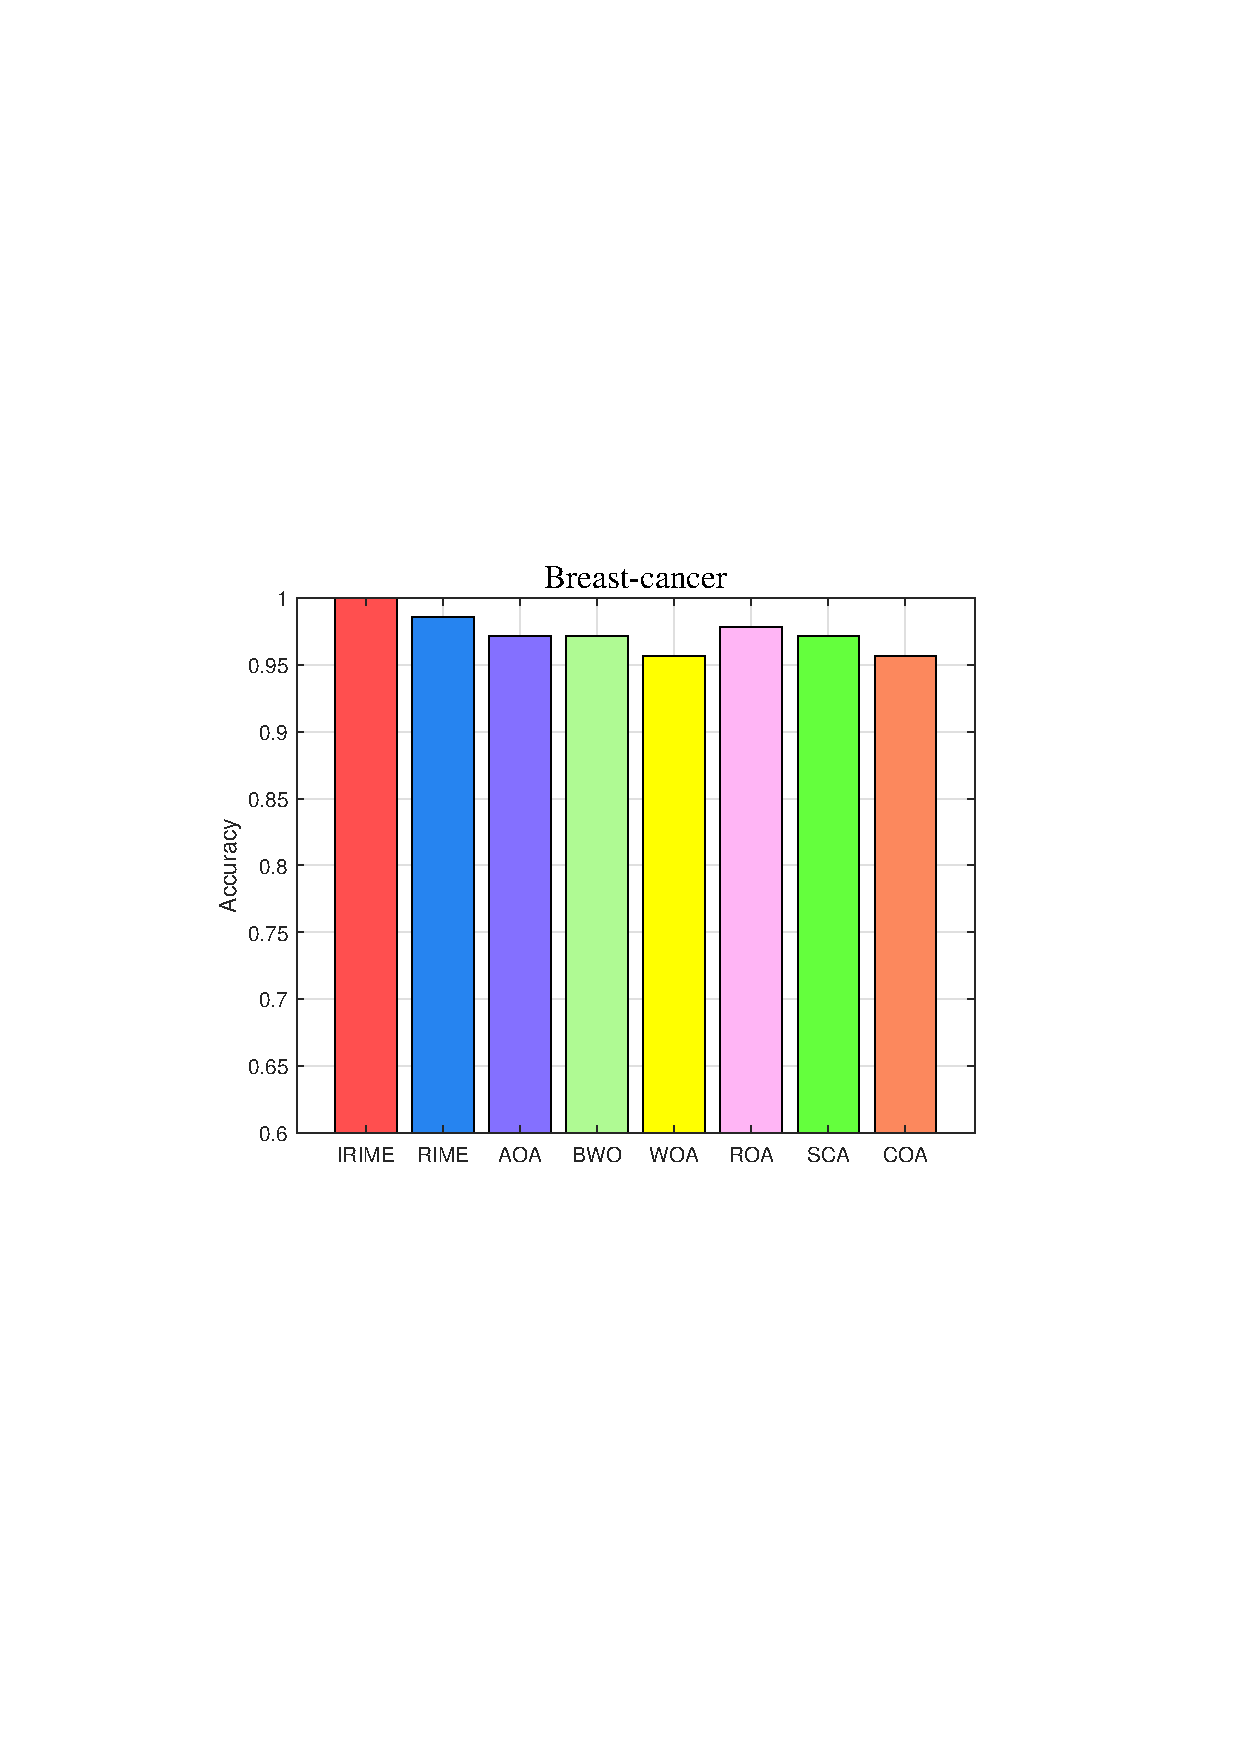
\includegraphics[width=\textwidth]{figures/FS/acc/2.pdf}
    \end{subfigure}
    \hfill
    \begin{subfigure}[b]{0.32\textwidth}
        \caption*{}
        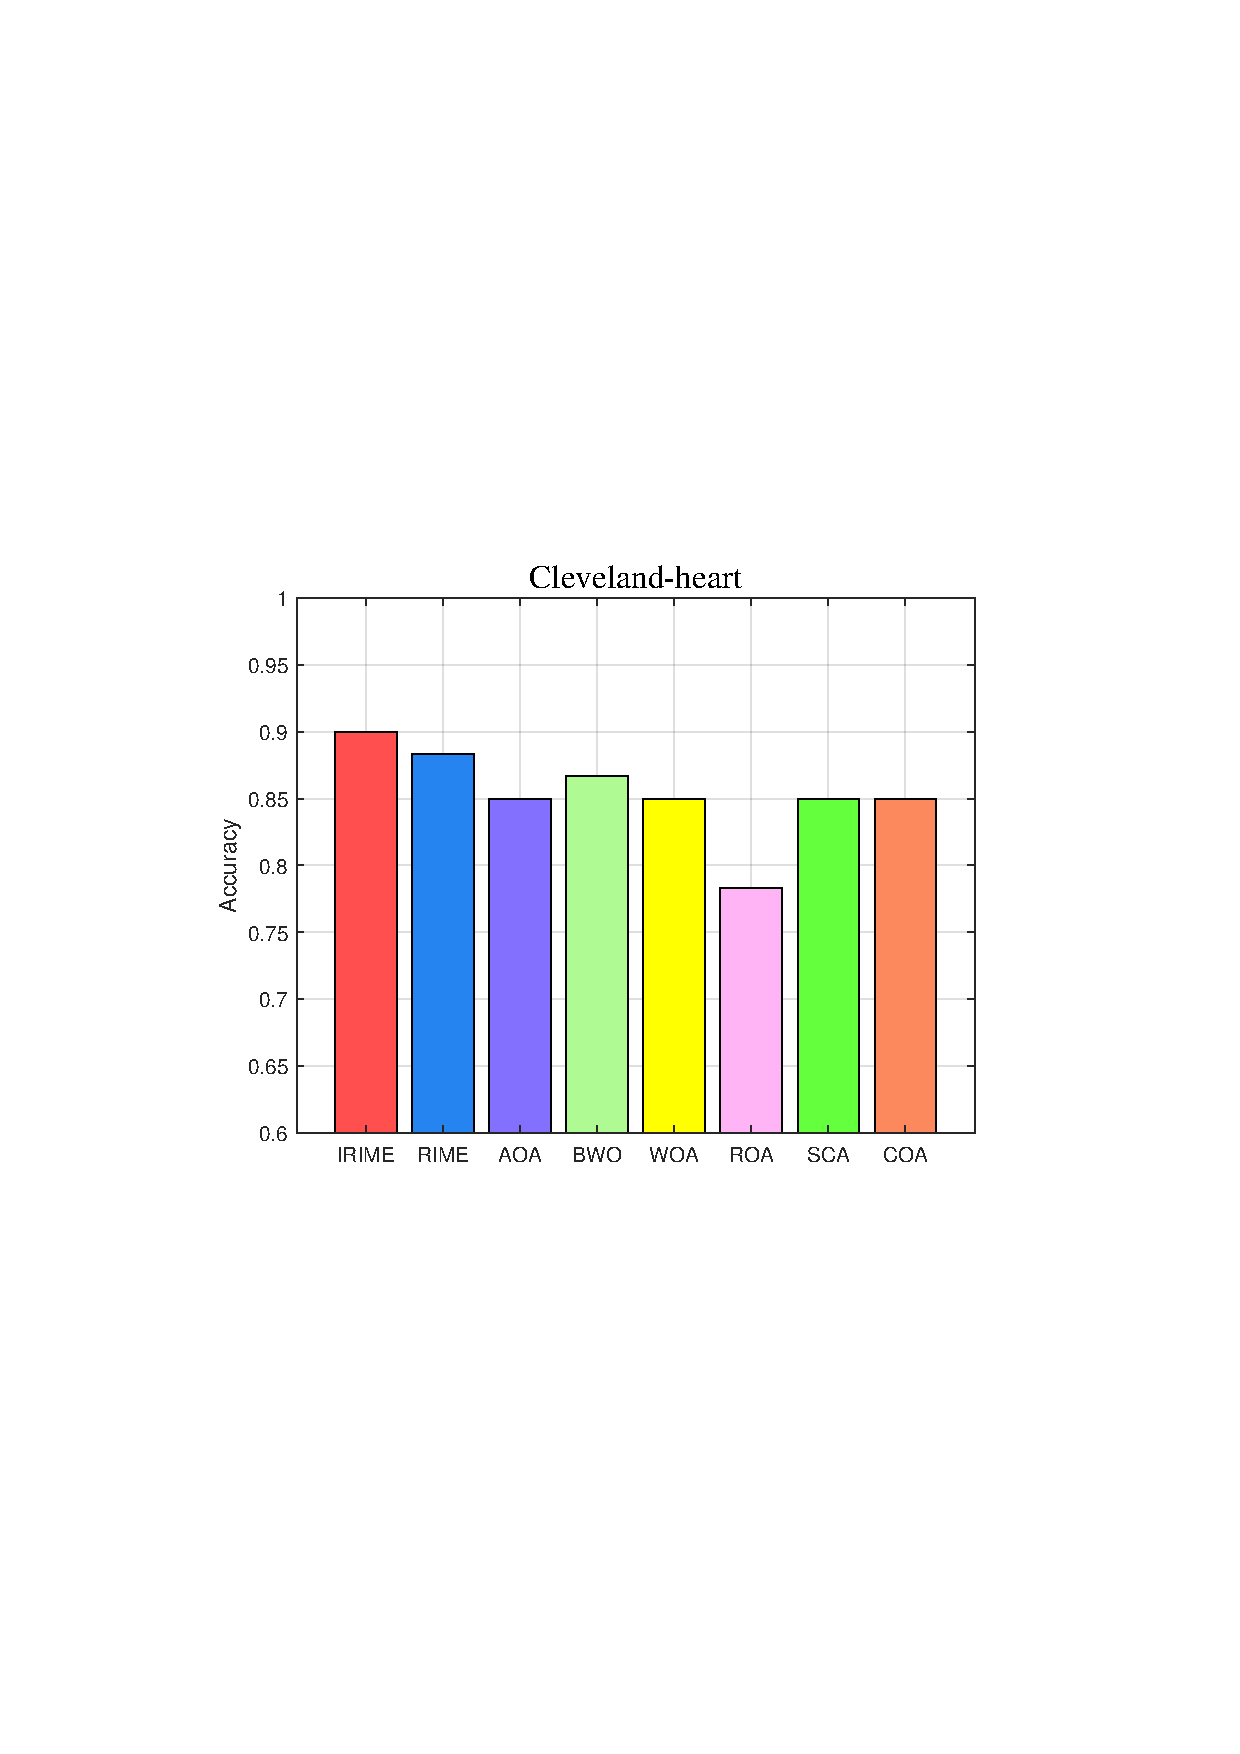
\includegraphics[width=\textwidth]{figures/FS/acc/3.pdf}
    \end{subfigure}
    % 第二行子图
    \begin{subfigure}[b]{0.32\textwidth}
        \caption*{}
        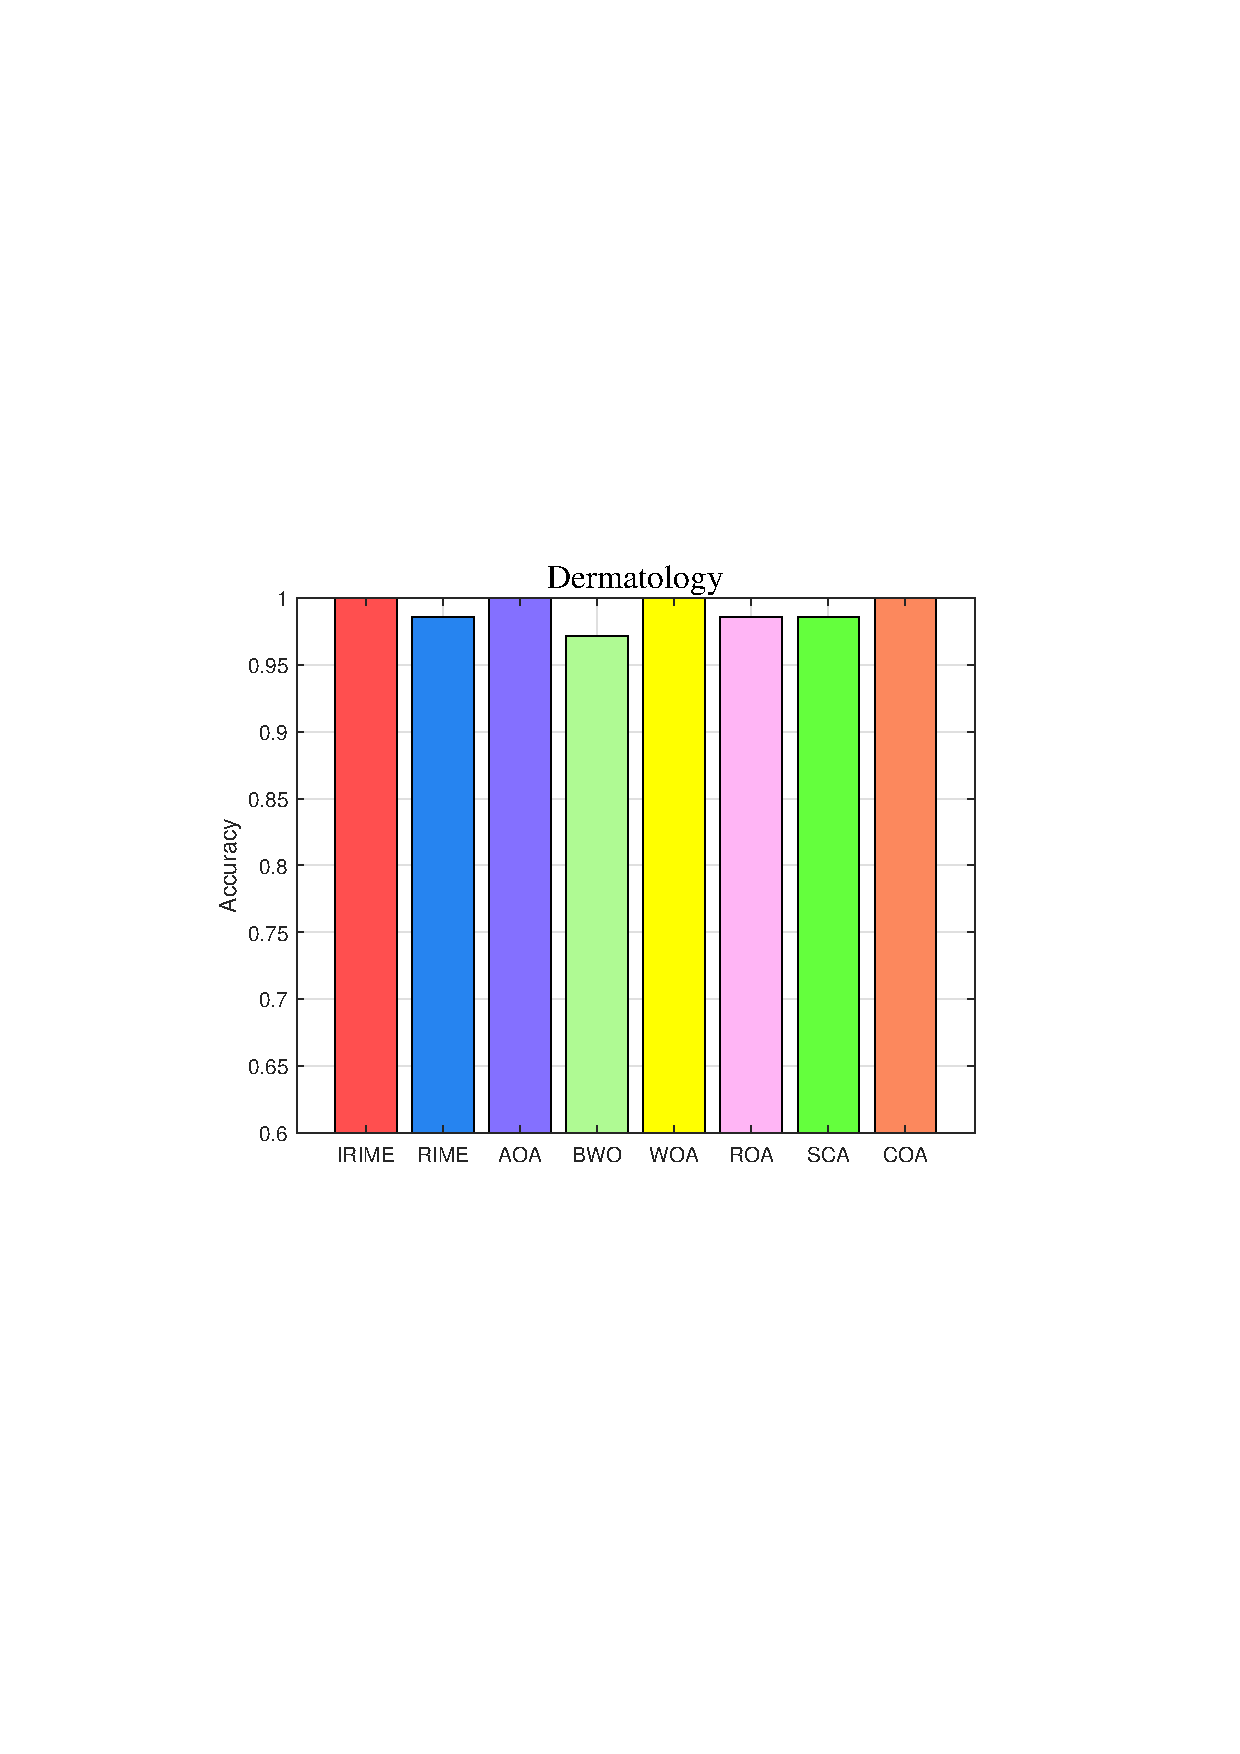
\includegraphics[width=\textwidth]{figures/FS/acc/4.pdf}
    \end{subfigure}
    \hfill
    \begin{subfigure}[b]{0.32\textwidth}
        \caption*{}
        
\includegraphics[width=\textwidth]{figures/FS/acc/5.pdf}
    \end{subfigure}
    \hfill
    \begin{subfigure}[b]{0.32\textwidth}
        \caption*{}
        
\includegraphics[width=\textwidth]{figures/FS/acc/6.pdf}
    \end{subfigure}
    % 第三行子图
    \begin{subfigure}[b]{0.32\textwidth}
        \caption*{}
        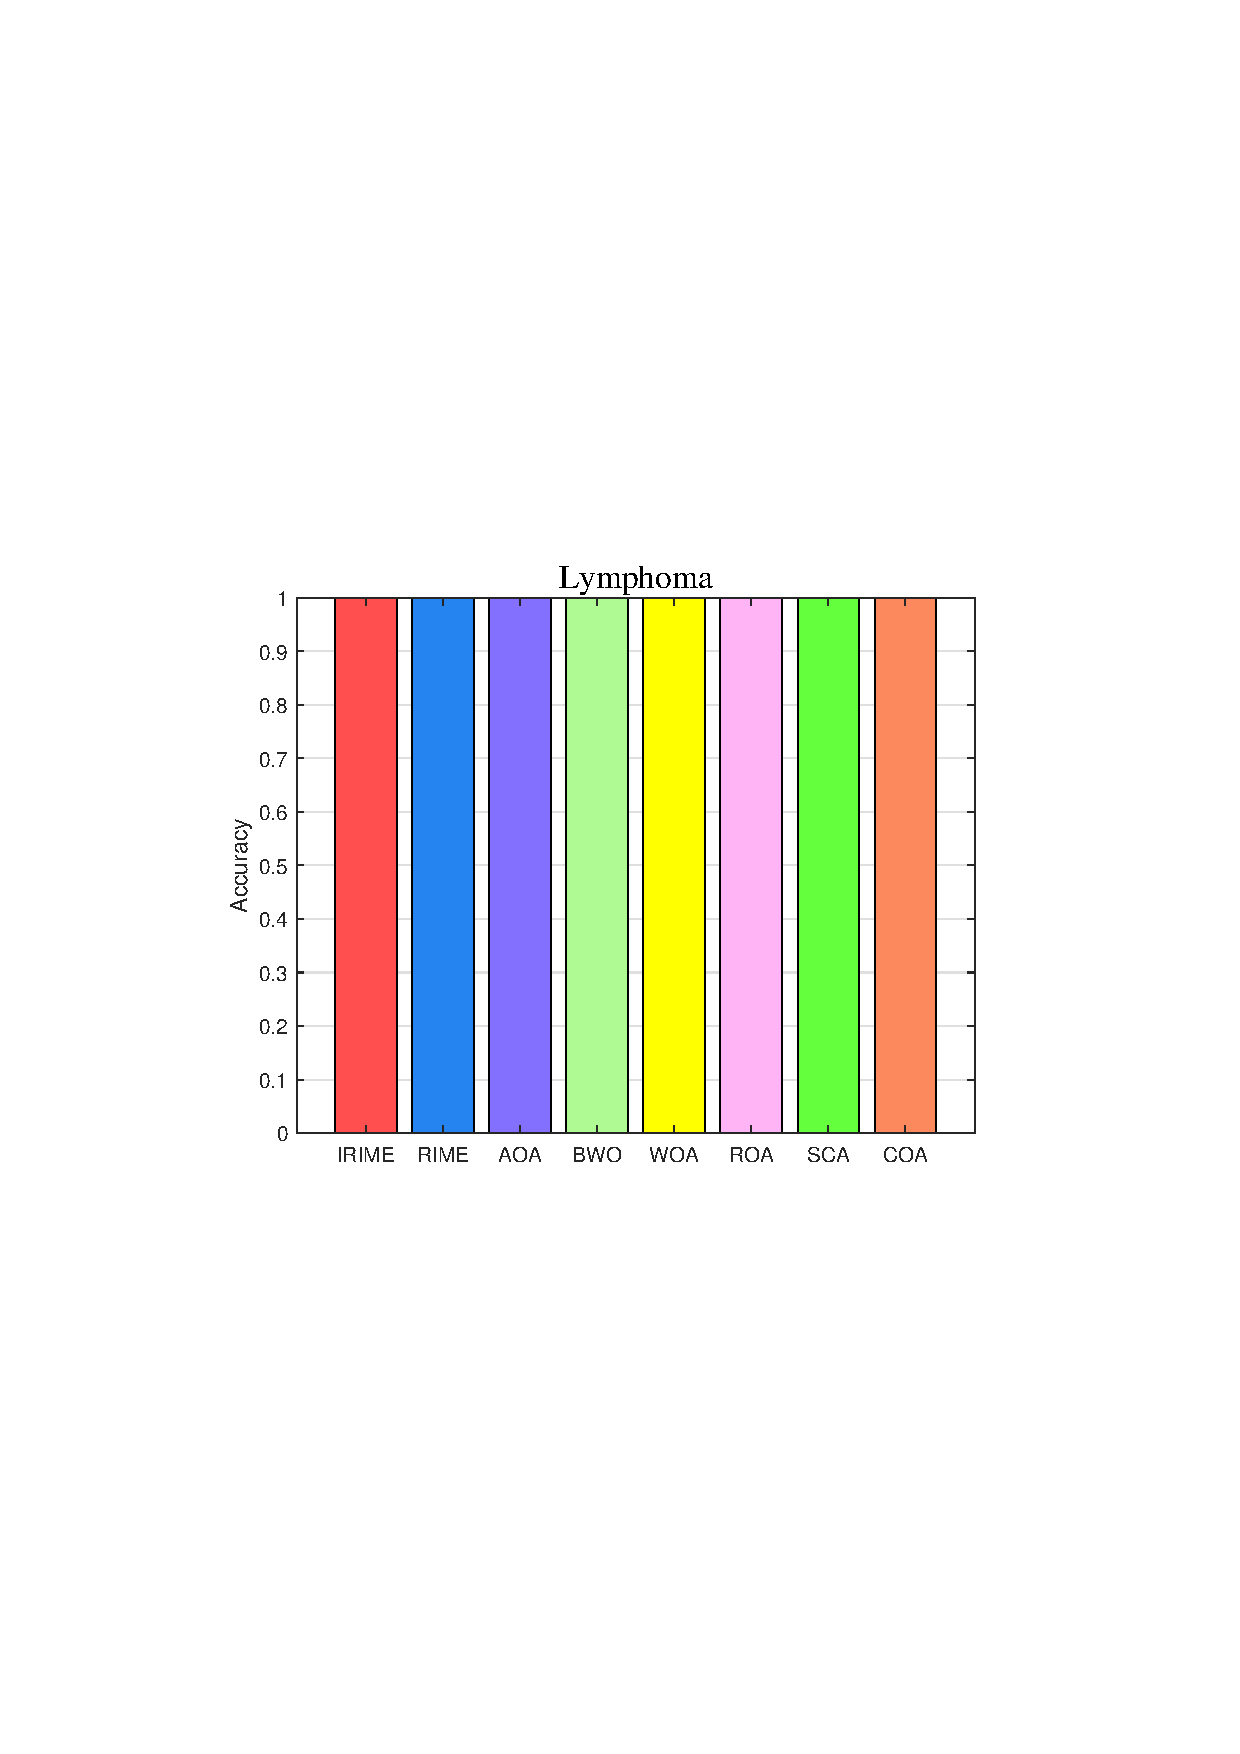
\includegraphics[width=\textwidth]{figures/FS/acc/7.pdf}
    \end{subfigure}
    \hfill
    \begin{subfigure}[b]{0.32\textwidth}
        \caption*{}
        
\includegraphics[width=\textwidth]{figures/FS/acc/8.pdf}
    \end{subfigure}
    \hfill
    \begin{subfigure}[b]{0.32\textwidth}
        \caption*{}
        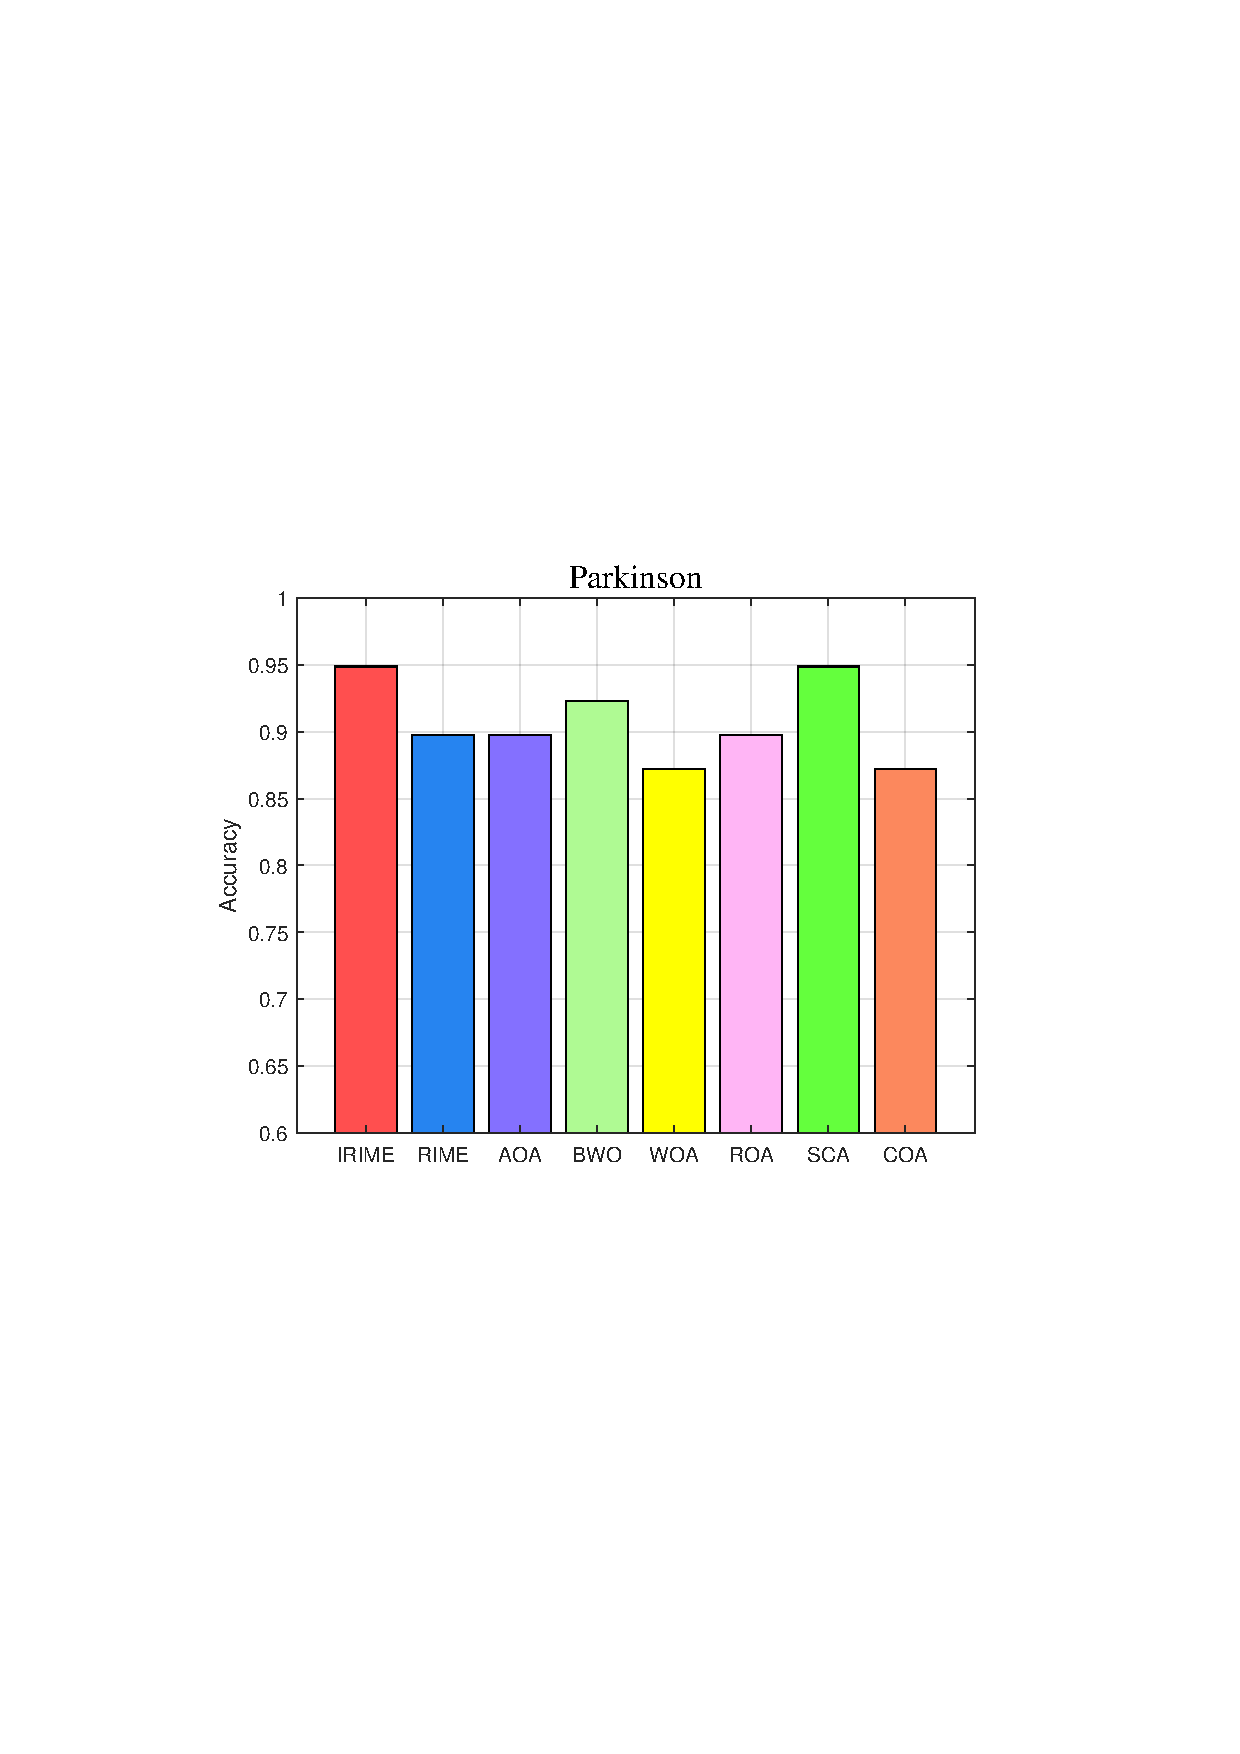
\includegraphics[width=\textwidth]{figures/FS/acc/9.pdf}
    \end{subfigure}
    % 第四行
    \begin{subfigure}[b]{0.32\textwidth}
        \caption*{}
        
\includegraphics[width=\textwidth]{figures/FS/acc/10.pdf}
    \end{subfigure}
    \hfill
    \begin{subfigure}[b]{0.32\textwidth}
        \caption*{}
        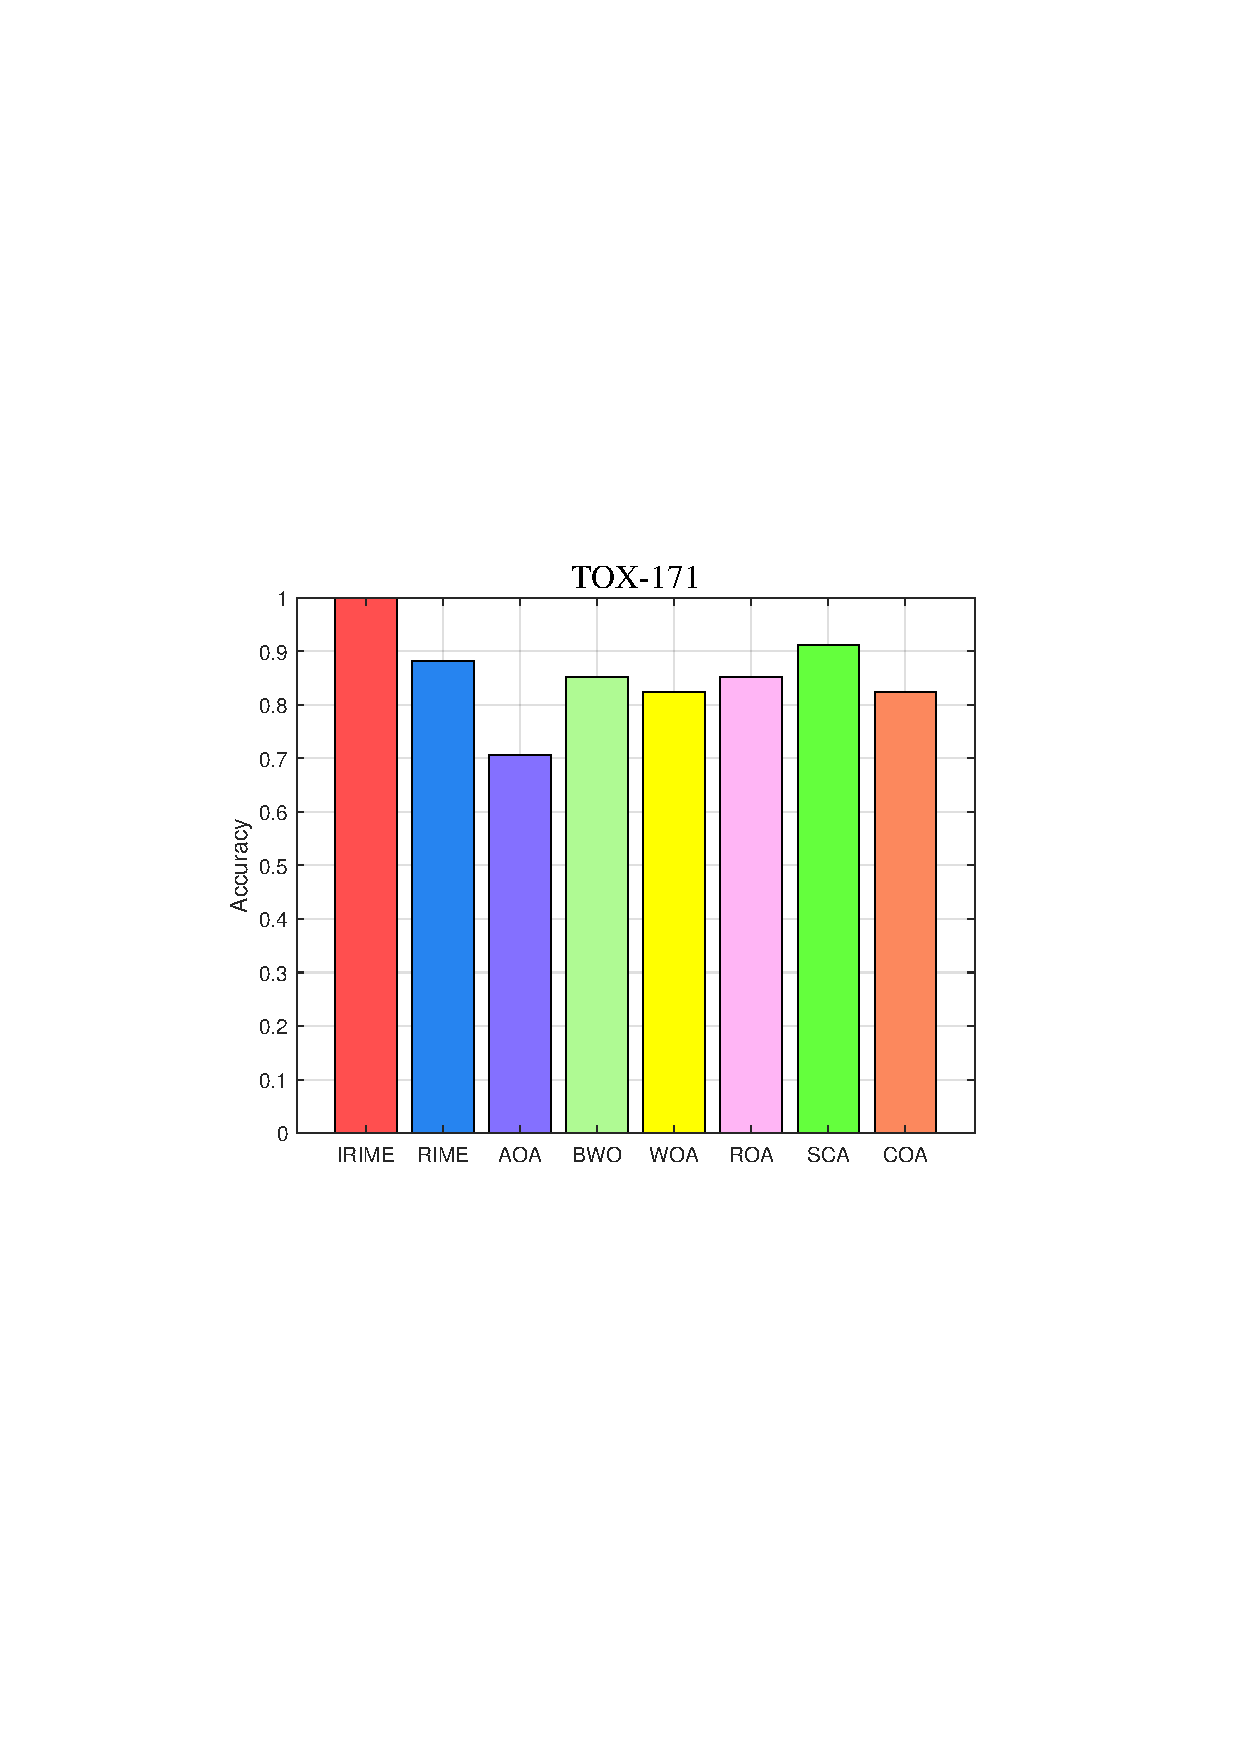
\includegraphics[width=\textwidth]{figures/FS/acc/11.pdf}
    \end{subfigure}
    \hfill
    \begin{subfigure}[b]{0.32\textwidth}
        \caption*{}
        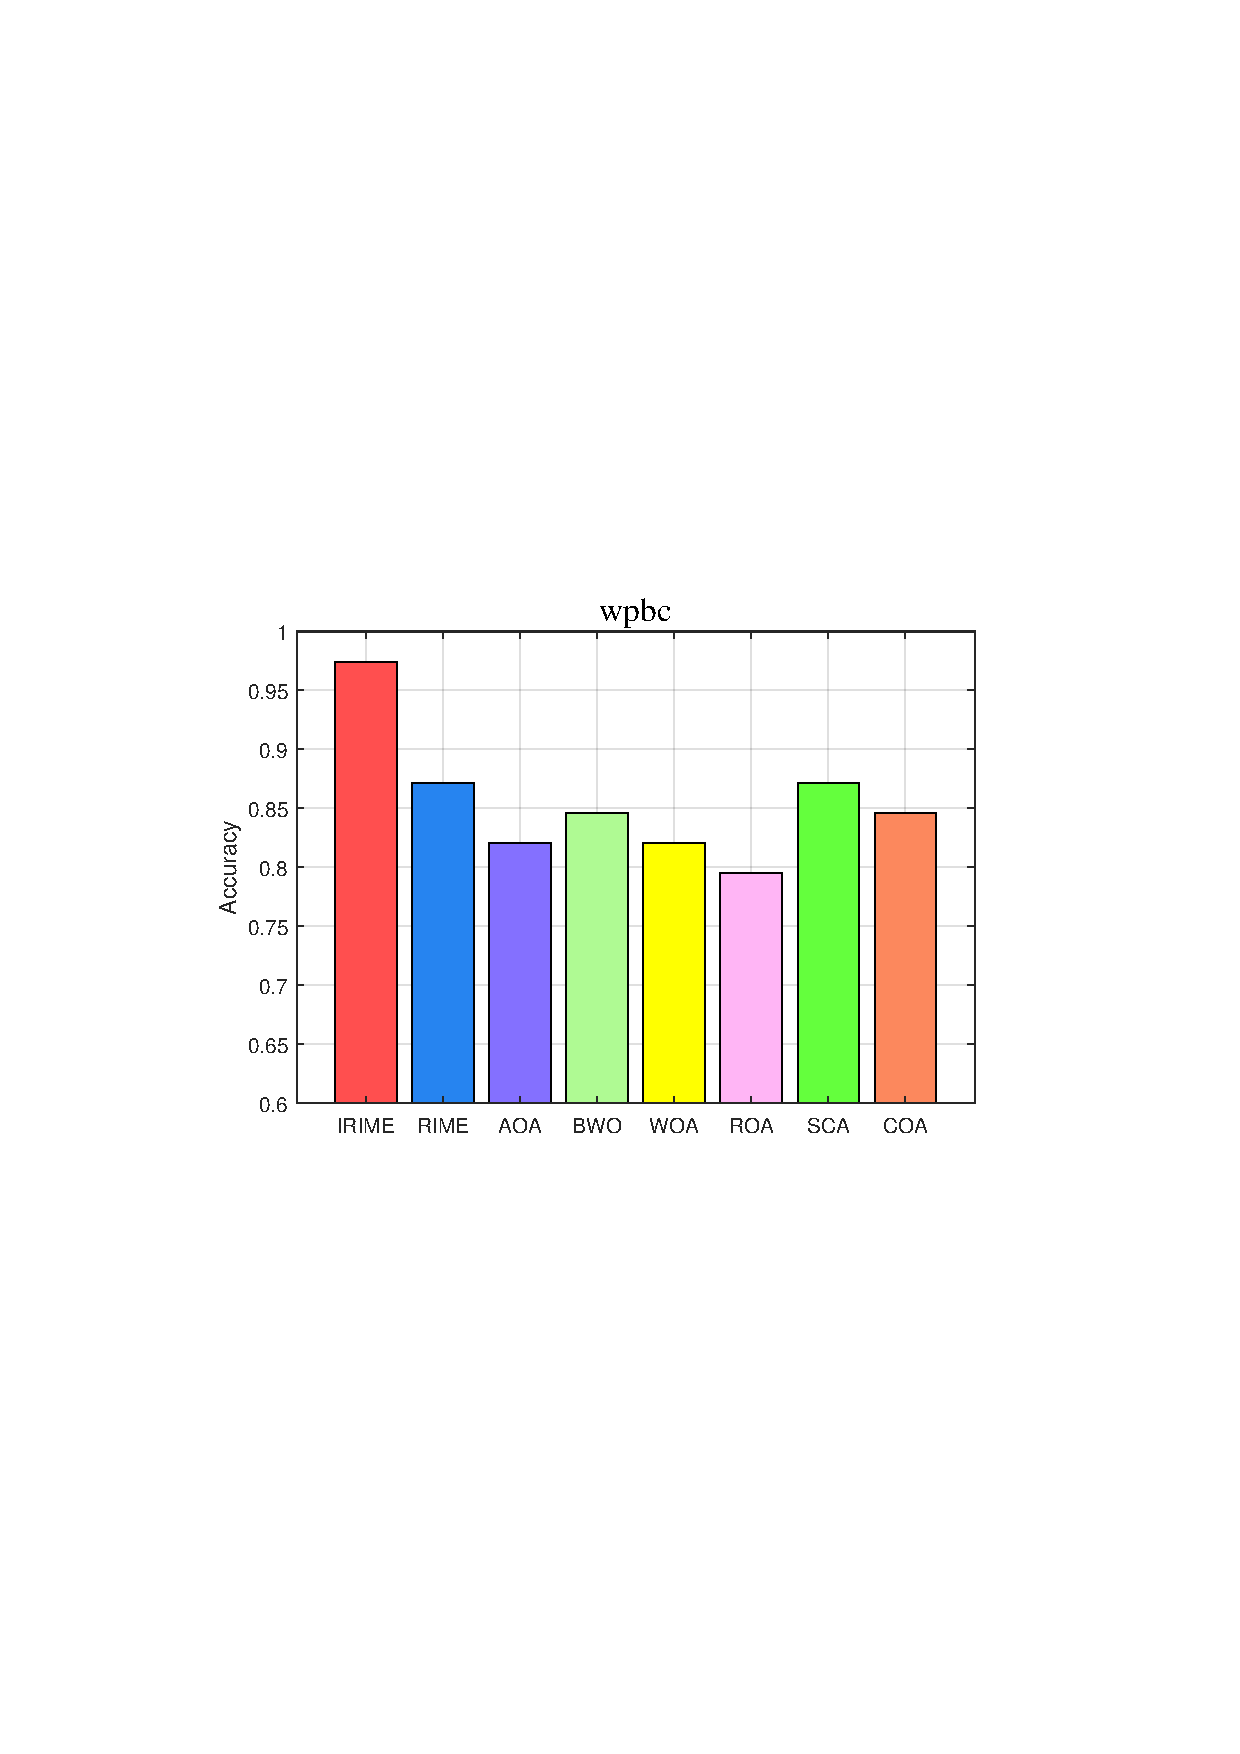
\includegraphics[width=\textwidth]{figures/FS/acc/12.pdf}
    \end{subfigure}
    \caption{12 个数据集上的对比准确率直方图}
    \label{fig:fs-acc}
\end{figure}

\begin{table}[htbp]
  \centering
  \caption{12 个数据集上的适应度值结果}
    \setlength{\tabcolsep}{3pt} % 减少列间距
    \tiny
    \begin{tabular}{cccccccccc}
    \toprule    
    Dataset & Metric & IRIME & RIME  & AOA   & BWO   & WOA   & ROA   & SCA   & COA \\
    \midrule
    \multirow{3}[0]{*}{Breast-cancer} & best  & 4.4444E-03 & 1.7578E-02 & 1.4900E-02 & 3.3333E-03 & 4.4444E-03 & 3.3333E-03 & 1.1567E-02 & 3.3333E-03 \\
          & mean  & 1.9624E-02 & 2.3028E-02 & 2.6478E-02 & 2.0336E-02 & 1.9689E-02 & 2.5877E-02 & 2.5432E-02 & 2.1159E-02 \\
          & std   & 1.1108E-02 & 5.5461E-03 & 1.1300E-02 & 1.1041E-02 & 1.1334E-02 & 1.0368E-02 & 1.1200E-02 & 1.2029E-02 \\
    \multirow{3}[0]{*}{Cleveland-heart} & best  & 6.9846E-02 & 6.9846E-02 & 8.7115E-02 & 5.3346E-02 & 8.8654E-02 & 3.8385E-02 & 6.9846E-02 & 5.5654E-02 \\
          & mean  & 1.0826E-01 & 1.1486E-01 & 1.2253E-01 & 1.2161E-01 & 1.2223E-01 & 1.0903E-01 & 1.1401E-01 & 1.1509E-01 \\
          & std   & 1.9192E-02 & 3.6574E-02 & 3.3669E-02 & 3.3271E-02 & 2.3424E-02 & 4.4835E-02 & 3.0825E-02 & 3.3782E-02 \\
    \multirow{3}[0]{*}{Dermatology} & best  & 1.7647E-03 & 2.3529E-03 & 4.1176E-03 & 5.0000E-03 & 3.8235E-03 & 3.8235E-03 & 1.4706E-03 & 3.2353E-03 \\
          & mean  & 4.2767E-03 & 7.3007E-03 & 1.3031E-02 & 1.5643E-02 & 1.1589E-02 & 1.4807E-02 & 1.1043E-02 & 6.6417E-03 \\
          & std   & 4.3719E-03 & 6.5224E-03 & 1.0056E-02 & 1.2877E-02 & 6.9351E-03 & 7.6337E-03 & 7.2608E-03 & 5.7978E-03 \\
    \multirow{3}[0]{*}{Diabetes} & best  & 1.6676E-01 & 1.7574E-01 & 1.6404E-01 & 1.8743E-01 & 1.8618E-01 & 2.0037E-01 & 1.9140E-01 & 2.0162E-01 \\
          & mean  & 2.0427E-01 & 2.1890E-01 & 2.2082E-01 & 2.1164E-01 & 2.1644E-01 & 2.3310E-01 & 2.1957E-01 & 2.1669E-01 \\
          & std   & 1.9885E-02 & 2.0106E-02 & 2.8935E-02 & 1.9926E-02 & 2.3074E-02 & 2.6184E-02 & 2.1388E-02 & 1.0460E-02 \\
    \multirow{3}[0]{*}{lungcancer-3class} & best  & 3.5714E-04 & 7.1429E-04 & 4.4643E-03 & 1.2500E-03 & 5.3571E-04 & 8.9286E-04 & 3.5714E-04 & 2.3214E-03 \\
          & mean  & 1.7214E-02 & 3.3964E-02 & 1.0418E-01 & 8.4339E-02 & 8.3839E-02 & 1.5043E-01 & 8.3143E-02 & 3.6054E-02 \\
          & std   & 5.2117E-02 & 6.9439E-02 & 1.3867E-01 & 1.1565E-01 & 1.1644E-01 & 1.2116E-01 & 8.7001E-02 & 6.9281E-02 \\
    \multirow{3}[0]{*}{Parkinson} & best  & 9.0909E-04 & 9.0909E-04 & 2.7657E-02 & 3.1818E-03 & 2.6748E-02 & 2.9476E-02 & 1.8182E-03 & 2.2727E-03 \\
          & mean  & 4.6692E-02 & 7.4570E-02 & 5.9892E-02 & 4.2115E-02 & 6.9902E-02 & 8.5678E-02 & 5.9703E-02 & 7.0266E-02 \\
          & std   & 2.6093E-02 & 4.8458E-02 & 3.3682E-02 & 2.0709E-02 & 2.7134E-02 & 3.5320E-02 & 3.1505E-02 & 3.7616E-02 \\
    \multirow{3}[0]{*}{SPECT} & best  & 7.8353E-02 & 5.9220E-02 & 9.9760E-02 & 6.2856E-02 & 8.3353E-02 & 7.9717E-02 & 7.7444E-02 & 4.3268E-02 \\
          & mean  & 1.0815E-01 & 1.1913E-01 & 1.2637E-01 & 1.4036E-01 & 1.2318E-01 & 1.2086E-01 & 1.1548E-01 & 1.0737E-01 \\
          & std   & 2.1731E-02 & 3.3873E-02 & 3.0181E-02 & 4.0193E-02 & 2.7183E-02 & 2.9275E-02 & 2.5141E-02 & 3.8726E-02 \\
    \multirow{3}[0]{*}{wpbc} & best  & 2.7506E-02 & 7.7972E-02 & 1.0730E-01 & 8.1608E-02 & 7.7366E-02 & 1.0366E-01 & 7.7063E-02 & 5.5315E-02 \\
          & mean  & 8.8429E-02 & 1.1161E-01 & 1.4347E-01 & 1.2696E-01 & 1.4672E-01 & 1.4056E-01 & 1.1064E-01 & 1.1811E-01 \\
          & std   & 3.6329E-02 & 2.3809E-02 & 3.3643E-02 & 2.4154E-02 & 3.1608E-02 & 2.6510E-02 & 2.4200E-02 & 5.0897E-02 \\
    \multirow{3}[0]{*}{ALLAML} & best  & 1.4027E-06 & 8.4163E-06 & 7.5650E-02 & 2.8054E-06 & 1.4027E-06 & 2.8054E-06 & 7.1539E-05 & 7.5319E-02 \\
          & mean  & 3.6471E-06 & 1.4210E-02 & 1.5397E-01 & 2.1221E-02 & 2.8295E-02 & 7.7909E-02 & 1.4248E-02 & 1.3198E-01 \\
          & std   & 1.5079E-06 & 2.9868E-02 & 5.2247E-02 & 3.4156E-02 & 3.6511E-02 & 7.0353E-02 & 2.9826E-02 & 6.4967E-02 \\
    \multirow{3}[0]{*}{Lymphoma} & best  & 2.4839E-06 & 4.9677E-06 & 4.7889E-03 & 2.4839E-06 & 4.9677E-06 & 7.4516E-06 & 7.4516E-06 & 7.6006E-04 \\
          & mean  & 4.7193E-06 & 7.2032E-06 & 4.8530E-03 & 2.9806E-06 & 8.9419E-06 & 1.7139E-05 & 1.5152E-05 & 4.1381E-03 \\
          & std   & 1.4100E-06 & 2.1749E-06 & 5.3077E-05 & 1.0473E-06 & 3.9186E-06 & 1.4024E-05 & 9.0281E-06 & 1.1887E-03 \\
    \multirow{3}[0]{*}{nci9} & best  & 1.6501E-01 & 2.4767E-01 & 4.1957E-01 & 2.4751E-01 & 2.4753E-01 & 3.3009E-01 & 2.4761E-01 & 4.1726E-01 \\
          & mean  & 2.7228E-01 & 3.4662E-01 & 5.5840E-01 & 3.6318E-01 & 3.6310E-01 & 4.5414E-01 & 3.4668E-01 & 5.5754E-01 \\
          & std   & 1.1034E-01 & 7.5740E-02 & 8.6980E-02 & 9.6622E-02 & 8.8655E-02 & 7.9960E-02 & 6.5048E-02 & 1.2324E-01 \\
    \multirow{3}[0]{*}{TOX-171} & best  & 1.6875E-04 & 3.2026E-02 & 1.5065E-01 & 8.7480E-02 & 3.1633E-02 & 6.4942E-02 & 2.9420E-02 & 6.3251E-02 \\
          & mean  & 3.5686E-02 & 9.5800E-02 & 2.2457E-01 & 1.5284E-01 & 1.3361E-01 & 1.5890E-01 & 7.6619E-02 & 1.3883E-01 \\
          & std   & 3.8437E-02 & 4.2697E-02 & 6.4879E-02 & 4.9116E-02 & 5.6303E-02 & 4.6560E-02 & 2.8391E-02 & 3.9287E-02 \\
    \bottomrule      
    \end{tabular}%
  \label{tb:FS-fitness}%
\end{table}%

\begin{table}[htbp]
  \centering
  \caption{12 个数据集上的准确率结果}
    \setlength{\tabcolsep}{3pt} % 减少列间距
    \tiny
    \begin{tabular}{cccccccccc}
    \toprule    
    Dataset & Metric & IRIME & RIME  & AOA   & BWO   & WOA   & ROA   & SCA   & COA \\
    \midrule
    \multirow{3}[0]{*}{Breast-cancer} & best  & 9.6403E-01 & 9.7122E-01 & 9.4964E-01 & 9.6403E-01 & 9.6403E-01 & 9.6403E-01 & 9.5683E-01 & 9.6403E-01 \\
          & mean  & 9.8489E-01 & 9.8201E-01 & 9.7842E-01 & 9.8417E-01 & 9.8561E-01 & 9.7914E-01 & 9.7914E-01 & 9.8345E-01 \\
          & std   & 1.0963E-02 & 5.0871E-03 & 1.2228E-02 & 1.0617E-02 & 1.1248E-02 & 9.8584E-03 & 1.1476E-02 & 1.1773E-02 \\
    \multirow{3}[0]{*}{Cleveland-heart} & best  & 8.6667E-01 & 8.1667E-01 & 8.3333E-01 & 8.3333E-01 & 8.5000E-01 & 8.5000E-01 & 8.1667E-01 & 8.5000E-01 \\
          & mean  & 8.9500E-01 & 8.8833E-01 & 8.8167E-01 & 8.8167E-01 & 8.8167E-01 & 8.9500E-01 & 8.8833E-01 & 8.8833E-01 \\
          & std   & 1.9325E-02 & 3.6893E-02 & 3.4650E-02 & 3.3747E-02 & 2.4152E-02 & 4.5168E-02 & 3.1476E-02 & 3.4292E-02 \\
    \multirow{3}[0]{*}{Dermatology} & best  & 9.8592E-01 & 9.8592E-01 & 9.7183E-01 & 9.5775E-01 & 9.8592E-01 & 9.8592E-01 & 9.8592E-01 & 9.8592E-01 \\
          & mean  & 9.9859E-01 & 9.9577E-01 & 9.9296E-01 & 9.9014E-01 & 9.9296E-01 & 9.9155E-01 & 9.9155E-01 & 9.9718E-01 \\
          & std   & 4.4539E-03 & 6.8035E-03 & 9.9593E-03 & 1.3362E-02 & 7.4232E-03 & 7.2732E-03 & 7.2732E-03 & 5.9385E-03 \\
    \multirow{3}[0]{*}{Diabetes} & best  & 7.5817E-01 & 7.5817E-01 & 7.4510E-01 & 7.5163E-01 & 7.5163E-01 & 7.5163E-01 & 7.4510E-01 & 7.7124E-01 \\
          & mean  & 7.8824E-01 & 7.8431E-01 & 7.8301E-01 & 7.9216E-01 & 7.8693E-01 & 7.8497E-01 & 7.8301E-01 & 7.8693E-01 \\
          & std   & 1.8538E-02 & 2.0897E-02 & 3.0314E-02 & 2.0391E-02 & 2.1830E-02 & 2.3756E-02 & 2.1743E-02 & 1.1610E-02 \\
    \multirow{3}[0]{*}{lungcancer-3class} & best  & 8.3333E-01 & 1.0000E+00 & 6.6667E-01 & 6.6667E-01 & 6.6667E-01 & 6.6667E-01 & 8.3333E-01 & 8.3333E-01 \\
          & mean  & 9.8333E-01 & 1.0000E+00 & 9.0000E-01 & 9.1667E-01 & 9.1667E-01 & 8.5000E-01 & 9.1667E-01 & 9.6667E-01 \\
          & std   & 5.2705E-02 & 0.0000E+00 & 1.4055E-01 & 1.1785E-01 & 1.1785E-01 & 1.2298E-01 & 8.7841E-02 & 7.0273E-02 \\
    \multirow{3}[0]{*}{Parkinson} & best  & 9.2308E-01 & 8.4615E-01 & 8.9744E-01 & 9.2308E-01 & 8.9744E-01 & 8.4615E-01 & 8.9744E-01 & 8.7179E-01 \\
          & mean  & 9.5385E-01 & 9.2564E-01 & 9.4359E-01 & 9.5897E-01 & 9.3077E-01 & 9.1538E-01 & 9.4103E-01 & 9.3077E-01 \\
          & std   & 2.6482E-02 & 4.9024E-02 & 3.3758E-02 & 2.1622E-02 & 2.7163E-02 & 3.6362E-02 & 3.2094E-02 & 3.8319E-02 \\
    \multirow{3}[0]{*}{SPECT} & best  & 8.6792E-01 & 8.1132E-01 & 8.3019E-01 & 7.9245E-01 & 8.3019E-01 & 8.3019E-01 & 8.4906E-01 & 8.3019E-01 \\
          & mean  & 8.9434E-01 & 8.8302E-01 & 8.7925E-01 & 8.6226E-01 & 8.8113E-01 & 8.8302E-01 & 8.8679E-01 & 8.9623E-01 \\
          & std   & 2.2147E-02 & 3.4218E-02 & 3.1067E-02 & 4.1766E-02 & 2.8197E-02 & 2.9230E-02 & 2.5157E-02 & 4.0025E-02 \\
    \multirow{3}[0]{*}{wpbc} & best  & 8.7179E-01 & 8.4615E-01 & 7.9487E-01 & 8.4615E-01 & 8.2051E-01 & 8.2051E-01 & 8.7179E-01 & 7.9487E-01 \\
          & mean  & 9.1282E-01 & 8.8974E-01 & 8.6154E-01 & 8.7436E-01 & 8.5385E-01 & 8.6154E-01 & 8.8974E-01 & 8.8462E-01 \\
          & std   & 3.6663E-02 & 2.4325E-02 & 3.4613E-02 & 2.5498E-02 & 3.2094E-02 & 2.7563E-02 & 2.4325E-02 & 5.1637E-02 \\
    \multirow{3}[0]{*}{ALLAML} & best  & 1.0000E+00 & 9.2857E-01 & 7.8571E-01 & 9.2857E-01 & 9.2857E-01 & 7.8571E-01 & 1.0000E+00 & 7.1429E-01 \\
          & mean  & 1.0000E+00 & 9.8571E-01 & 8.5000E-01 & 9.7857E-01 & 9.7143E-01 & 9.2143E-01 & 1.0000E+00 & 8.7143E-01 \\
          & std   & 0.0000E+00 & 3.0117E-02 & 5.2705E-02 & 3.4503E-02 & 3.6886E-02 & 7.1031E-02 & 0.0000E+00 & 6.5638E-02 \\
    \multirow{3}[0]{*}{Lymphoma} & best  & 1.0000E+00 & 1.0000E+00 & 1.0000E+00 & 1.0000E+00 & 1.0000E+00 & 1.0000E+00 & 1.0000E+00 & 1.0000E+00 \\
          & mean  & 1.0000E+00 & 1.0000E+00 & 1.0000E+00 & 1.0000E+00 & 1.0000E+00 & 1.0000E+00 & 1.0000E+00 & 1.0000E+00 \\
          & std   & 0.0000E+00 & 0.0000E+00 & 0.0000E+00 & 0.0000E+00 & 0.0000E+00 & 0.0000E+00 & 0.0000E+00 & 0.0000E+00 \\
    \multirow{3}[0]{*}{nci9} & best  & 5.0000E-01 & 5.0000E-01 & 3.3333E-01 & 5.0000E-01 & 5.0000E-01 & 4.1667E-01 & 5.8333E-01 & 1.6667E-01 \\
          & mean  & 7.2500E-01 & 6.5000E-01 & 4.7500E-01 & 6.3333E-01 & 6.3333E-01 & 5.4167E-01 & 6.5000E-01 & 4.4167E-01 \\
          & std   & 1.1146E-01 & 7.6578E-02 & 9.6625E-02 & 9.7816E-02 & 8.9581E-02 & 8.0985E-02 & 6.5734E-02 & 1.2454E-01 \\
    \multirow{3}[0]{*}{TOX-171} & best  & 8.8235E-01 & 8.8235E-01 & 7.0588E-01 & 7.9412E-01 & 7.9412E-01 & 7.9412E-01 & 8.8235E-01 & 8.2353E-01 \\
          & mean  & 9.6471E-01 & 9.4412E-01 & 8.0294E-01 & 8.4706E-01 & 8.6765E-01 & 8.4412E-01 & 9.2353E-01 & 8.6471E-01 \\
          & std   & 3.8722E-02 & 2.9248E-02 & 6.0515E-02 & 4.9604E-02 & 5.7585E-02 & 4.8129E-02 & 2.8414E-02 & 3.9703E-02 \\
    \bottomrule      
    \end{tabular}%
  \label{tb:FS-acc}%
\end{table}%

%特征选择featureSize图
\begin{figure}[htbp]
    \centering
    % 第一行子图
    \begin{subfigure}[b]{0.32\textwidth}
        \caption*{}
        
\includegraphics[width=\textwidth]{figures/FS/feature/1.pdf}
    \end{subfigure}
    \hfill
    \begin{subfigure}[b]{0.32\textwidth}
        \caption*{}
        
\includegraphics[width=\textwidth]{figures/FS/feature/2.pdf}
    \end{subfigure}
    \hfill
    \begin{subfigure}[b]{0.32\textwidth}
        \caption*{}
        
\includegraphics[width=\textwidth]{figures/FS/feature/3.pdf}
    \end{subfigure}
    % 第二行子图
    \begin{subfigure}[b]{0.32\textwidth}
        \caption*{}
        
\includegraphics[width=\textwidth]{figures/FS/feature/4.pdf}
    \end{subfigure}
    \hfill
    \begin{subfigure}[b]{0.32\textwidth}
        \caption*{}
        
\includegraphics[width=\textwidth]{figures/FS/feature/5.pdf}
    \end{subfigure}
    \hfill
    \begin{subfigure}[b]{0.32\textwidth}
        \caption*{}
        
\includegraphics[width=\textwidth]{figures/FS/feature/6.pdf}
    \end{subfigure}
    % 第三行子图
    \begin{subfigure}[b]{0.32\textwidth}
        \caption*{}
        
\includegraphics[width=\textwidth]{figures/FS/feature/7.pdf}
    \end{subfigure}
    \hfill
    \begin{subfigure}[b]{0.32\textwidth}
        \caption*{}
        
\includegraphics[width=\textwidth]{figures/FS/feature/8.pdf}
    \end{subfigure}
    \hfill
    \begin{subfigure}[b]{0.32\textwidth}
        \caption*{}
        
\includegraphics[width=\textwidth]{figures/FS/feature/9.pdf}
    \end{subfigure}
    % 第四行
    \begin{subfigure}[b]{0.32\textwidth}
        \caption*{}
        
\includegraphics[width=\textwidth]{figures/FS/feature/10.pdf}
    \end{subfigure}
    \hfill
    \begin{subfigure}[b]{0.32\textwidth}
        \caption*{}
        
\includegraphics[width=\textwidth]{figures/FS/feature/11.pdf}
    \end{subfigure}
    \hfill
    \begin{subfigure}[b]{0.32\textwidth}
        \caption*{}
        
\includegraphics[width=\textwidth]{figures/FS/feature/12.pdf}
    \end{subfigure}
    \caption{12 个数据集上的对比特征数量直方图}
    \label{fig:fs-feature1}
\end{figure}

\subsection{消融实验}
本实验对IRIME所提出的改进策略进行系统性地进行消融研究，以评估IRIME中三项关键策略的单独贡献： (1) 信息熵评估策略，(2) 随机重启机制，(3) 拉格朗日插值法。实验结果显示不同策略组合具有明显的性能模式。我们将表7中的四个算法用于消融实验。对比结果显示性能差异显著：完整的IRIME取得了优异的表现，最终排名得分优于所有部分变体。详细排名结果如图8所示，结合表5和表6的对比实验详细结果，我们可以得出以下结论：
拉格朗日插值法：最具影响力的组成部分，特别是在43\%的单模态函数（平均提升62.3\%）和组合函数（58.1\%）中。其多项式逼近能力显著加快了收敛速度。
随机重启机制：维持种群多样性、防止早熟收敛的关键，在87\%的多模态情况下发挥作用。典型例子包括F18（1.4对4.0的得分差异）。
信息熵评估策略：在特定函数类别中提供了选择性优势，特别增强了可分离函数的开发能力（F1-F3表现出18.7\%的性能提升）。
这些结果共同验证了每个策略对IRIME性能的独特贡献，其中拉格朗日插值法是最关键的组成部分，其次是随机重启机制和信息熵评估策略，影响程度依次递减。
\begin{figure}[htbp]
    \centering
    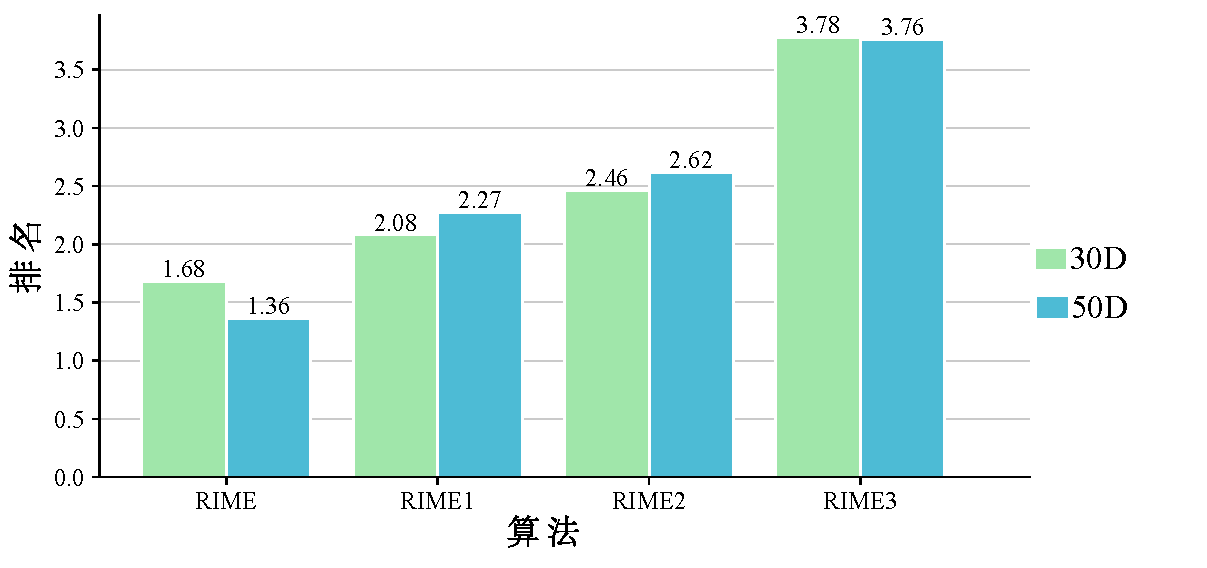
\includegraphics[width=1.0\linewidth]{figures/Ftest/Ftest-ablation.pdf} % 调整宽度为适合您文档的值
    \caption{IRIME 及其变体的 Friedman 检验结果}
    \label{fig:Ftest-ablation}
\end{figure}
\begin{table}[htbp]
  \centering
  \small
  \caption{IRIME 变体详情 ('Y' = 使用策略 ; 'N' = 未使用)}
  \begin{tabular}{lcccc}
    \toprule
    & RIME & RIME1 & RIME2 & RIME3 \\
    \midrule
    Information entropy evaluation strategy   & Y & N & Y & Y\\
    Lagrange interpolation method  & Y & Y & N & Y\\
    Random restart mechanism  & Y & Y & Y & N \\
    \bottomrule
  \end{tabular}
\label{tb:variant IRIME}
\end{table}


\section{本章小结}
本章围绕多策略融合改进的雾凇算法（IRIME）展开研究，通过算法设计、实验验证与策略有效性分析完成系统性探索。
算法层面，提出三项核心改进策略：信息熵评估策略通过量化各维度不确定性分配动态权重，平衡优化过程中的探索与利用；拉格朗日插值法基于三维节点构建多项式近似，快速逼近最优解，提升局部搜索精度；随机重启机制通过随机化迭代阈值，刷新适应度靠后的个体，维持种群多样性并避免早熟收敛。三者与原始雾凇算法融合，形成完整的 IRIME 优化框架，其时间复杂度主要由种群规模、问题维度、迭代次数及评估函数计算成本决定。
实验设计包含三类验证场景：CEC 2017 基准函数对比实验中，IRIME 与八种先进算法在 30 维及 50 维环境下进行测试，通过收敛曲线、箱线图及弗里德曼统计检验，证实其在单模态、多模态、混合及组合函数上均具备更优的收敛速度、解质量与稳定性；医学数据集特征选择实验中，针对 12 个不同维度的医学数据集，IRIME 在分类准确率、适应度值及特征筛选效率上表现突出，尤其在高维数据集上展现出强大的特征降维与分类性能；消融实验通过系统性移除三项改进策略，明确了拉格朗日插值法对收敛速度的关键提升作用、随机重启机制在维持多样性中的核心价值，以及信息熵评估策略对特定函数类别的优化增益，验证了各策略的必要性与协同效应。
整体而言，IRIME 通过多策略的合理融合与协同，有效提升了优化算法的综合性能，在理论优化与实际医学特征选择问题中均展现出显著优势。

\chapter{基于多策略改进的哈里斯鹰算法}


\section{算法介绍}

\subsection{经验互益策略}
HHO算法个体位置更新的主要依据是种群当前的状态以及最优个体的位置信息。该方法在初探时能很好地保持搜索范围的宽与深。随着进化轮次的增多，由于种群个体间信息交流的单一化，群体多样性变小，从而导致算法很快会陷入局部最优解中。尤其是到了中期阶段，仅仅依靠代内交互不能很好地利用历史经验积累的有效信息，导致持续优化的效果不好。由此本文引入经验互益策略[7]，它加强了种群对于过去搜索过程中的重要经验，提高了个体之间的合作水平。该策略的关键之处就在于把历史种群所拥有的经验数据转化成引导向量加入到当下的个体状态更新当中，从而提升个体跳出局部最优的潜能以及拓展解空间的探寻幅度。由于算法早期需要具有较高的随机性才能找到潜在的全局最优解，在探索和开发阶段的过渡区间里才使用该种经验互益策略。
为了描述历史经验对当前个体的作用，首先保存上一代种群的位置矩阵H。对于当前个体Xi，随机选取3个历史个体索引r1、r2和r3，并逐维构造3个经验向量${\mathrm{E}}_{1}^{\mathrm{h}}$、${\mathrm{E}}_{2}^{\mathrm{h}}$ 和 ${\mathrm{E}}_{3}^{\mathrm{h}}$。其第$d$维可表示为：
\begin{equation}
    {E}_{1,d}^{h} = \left\{  \begin{array}{ll} {H}_{{r}_{1},d}, & \text{ rand } < {p}_{h} \\  {X}_{i,d}, & \text{ 其他 } \end{array}\right.
\end{equation}

\begin{equation}
    {E}_{2,d}^{h} = \left\{  \begin{array}{ll} {H}_{{r}_{2},d}, & \text{ rand } < {p}_{h} \\  {X}_{i,d}, & \text{ 其他 } \end{array}\right.
\end{equation}

\begin{equation}
    {E}_{3,d}^{h} = \left\{  \begin{array}{ll} {H}_{{r}_{3},d}, & \text{ rand } < {p}_{h} \\  {X}_{i,d}, & \text{ 其他 } \end{array}\right.
\end{equation}

其中, ${p}_{h}$ 为历史经验继承概率。
根据上述公式可知, 个体按照一定概率继承历史种群的经验信息, 否则保持现状。既可以使个体不偏离当前搜索路径, 又可以很好地将以前的经验加以整合。为了保证经验共享策略在优化中起到主导作用, 采用权重因子 ${w}_{t}$ 的方式进行计算,其计算公式为:
\begin{equation}
    {w}_{t} = 1 - \frac{\left| 2 \times  \frac{t}{T} - 1\right| }{0.4}
\end{equation}

其中, $t$ 为当前评估次数, $T$ 为最大评估次数。

当 ${w}_{t} < 0$ 时,令 ${w}_{t} = 0$ 。权重值在搜索初期慢慢提高,在后期却慢慢地降低,以此来达到经验协同策略在某些时期的有效控制目的。在此基础上, 构造经验互益候选解如下公式所示。

\begin{equation}
    {X}_{\text{ embs }} = {X}_{i} + {w}_{t} \times  \left( {\alpha  \times  R \times  \left( {{E}_{1}^{h} - {X}_{i}}\right)  + \beta  \times  \left( {1 - R}\right)  \times  \left( {{E}_{2}^{h} - {E}_{3}^{h}}\right) }\right)
\end{equation}

其中, $\mathrm{R}$ 为 $\left\lbrack  {0,1}\right\rbrack$ 上的随机向量, $a$ 和 $\beta$ 分别为经验受益项与经验互补项的权重系数。

为了使经验互益策略与传统的 HHO 算法的位置更新机制互相配合工作，需要把经验互益策略产生出的候选解同 HHO 算法得到的初始候选解 ${X}_{H}$ 进行融合,从而得到改进后的经验互益候选解。融合过程可以使用如下数学式子来表示。

\begin{equation}
    {X}_{\text{ embs }}^{\text{ final }} = {X}_{H} + {w}_{t}\left( {{X}_{\text{ embs }} - {X}_{i}}\right)
\end{equation}
\subsubsection{策略设计背景与动机}
元启发式算法（Meta-heuristic Algorithms, MAs）在搜索过程中，种群位置的频繁迭代更新往往导致算法迅速转向新的搜索区域。这种机制虽然保证了探索范围，但容易导致对原始高质量区域的挖掘深度不足，且个体与种群之间的“搜索经验”传递效率较低。

受人类社会“群体学习与经验总结”模式的启发，本章引入一种名为经验交流策略（Experience Exchange Strategy, EES）的进化算子。EES 的核心逻辑是将算法在演化过程中获取的位置视为“学习经验”，通过加强个体与种群间的联系，将搜索过程动态划分为三个阶段，旨在通过经验的积累与交换来平衡算法的全局勘探（Exploration）与局部开发（Exploitation）能力。

\subsubsection{EES 数学模型与阶段划分}
EES 策略将整个进化过程（最大迭代次数为 $T$）分为三个逻辑阶段：经验匮乏阶段（ESC）、经验交叉阶段（ECR）和经验共享阶段（ESH）。

\paragraph{经验匮乏阶段 (Experience Scarcity Stage, ESC)}
在算法搜索初期（$t < T/3$），种群积累的经验较少。此时策略的重点是保持原算法的探索特性，同时引入初步的经验干扰以避免早期停滞。其更新公式如下：
\begin{equation}
X_{new}(t) = X_{orig}(t) + r_1 \cdot (X_{exp1} - X_{exp2})
\end{equation}
其中：
\begin{itemize}
\item $X_{orig}(t)$ 表示由基础元启发式算法生成的原始位置。
\item $X_{exp1}$ 和 $X_{exp2}$ 是从当前经验池中随机选择的两个经验个体。
\item $r_1$ 为 $[0, 1]$ 之间的随机数。
\end{itemize}

\paragraph{经验交叉阶段 (Experience Crossover Stage, ECR)}
当算法进入中期（$T/3 \le t < 2T/3$），种群已探索了多个区域并积累了一定经验。此时为了跳出局部最优，EES 引入更多个体的经验交换：
\begin{equation}
X_{new}(t) = X_{exp\_best} + r_2 \cdot (X_{exp1} - X_{exp2}) + r_3 \cdot (X_{exp3} - X_{i}(t))
\end{equation}
在此阶段，个体通过与三个随机经验个体（$X_{exp1}, X_{exp2}, X_{exp3}$）以及当前个体 $X_i$ 的交叉更新，增强了信息流动的多样性，提高了搜索空间的覆盖精度。

\paragraph{经验共享阶段 (Experience Sharing Stage, ESH)}
在搜索后期（$t \ge 2T/3$），种群已经识别出潜在的最优区域。此时 EES 切换至高强度的信息共享模式，通过聚合群体智慧进行精细化搜索：
\begin{equation}
X_{new}(t) = \frac{X_{best} + X_{exp1} + X_{exp2} + X_{exp3}}{4}
\end{equation}
通过计算当前全局最优个体 $X_{best}$ 与多个经验个体的平均位置，算法能够显著增强局部开发强度，提高最终解的收敛精度。

\begin{enumerate}
\item ESC 阶段：侧重于全局探索，利用少量经验差值保持种群活力。
\item ECR 阶段：通过中等强度的经验交叉，辅助算法在复杂的解空间中跳出局部极值点。
\item ESH 阶段：利用群体经验的聚合效应，引导所有个体向全局最优解快速收敛。
\end{enumerate}
这种阶梯式的经验交换机制不仅增强了算法的稳健性，也为不同类型的元启发式算法提供了一个通用的性能增强框架。

\subsection{能量自适应柯西-高斯扰动策略}
在原始 HHO 中, 算法通过逃逸能量 E 控制探索阶段与开发阶段的切换。虽然逃逸能量可以反映当前的搜索状态, 但是它的位置扰动方式比较固定, 缺少根据动态变化的搜索情景来调节扰动模式的功能。为了提高全局搜索的效率, 在开始的时候就要扩大搜索范围, 在后期逐渐减小搜索步长来加强局部优化精度。单一种类的干扰方式很难达到早期广域探索和后期精确局部开垦两个目的。本文提出一种能量自适应调节的 Cauchy-Gaussian 混合扰动策略。此方法用 Cauchy 分布的重尾性提高远距离随机跳跃的能力, 用 Gaussian 分布的正态化平稳性达到高精度局部搜索的效果。利用实时观测到的逃逸能量变化情况, 自主地对两种扰动分量所占比例予以改变, 进而改善算法在全局搜索同局部改进两者之间所取得的结果表现状况。如下图X所示。

首先，根据逃逸能量构造归一化权重如下公式所示：
\begin{equation}
    \omega  = \min \left( {1,\frac{\left| E\right| }{2}}\right)
\end{equation}

其中, $E$ 为当前个体对应的逃逸能量。
当 $\left| E\right|$ 较大时, $\omega$ 较大,说明当前个体更倾向于执行全局探索; 当 $\left| E\right|$ 较小时, $\omega$ 较小,说明当前个体更倾向于局部开发。随后,从当前种群中随机选取一个个体 ${X}_{r}$ ,并分别生成 Cauchy 随机向量 $C$ 与 Gaussian 随机向量 $G$ 。为了使 Gaussian 扰动在搜索后期逐渐减弱,其扰动尺度设置如下公式所示。
\begin{equation}
    {\sigma }_{t} = {\sigma }_{0} \times  \left( {1 - \frac{t}{T}}\right) 
\end{equation}
其中, $\sigma$ 为 Gaussian 扰动的初始尺度参数。
之后, 使用公式 (23) 构造能量自适应 Cauchy-Gaussian 扰动候选解。
\begin{equation}
    {X}_{cg} = {X}_{i} + \omega  \times  C \times  \left( {{X}_{i} - {X}_{r}}\right)  + \left( {1 - \omega }\right)  \times  G \times  \left( {{X}_{\text{ rabbit }} - {X}_{i}}\right)
\end{equation}

其中, ${X}_{i}$ 表示当前个体, ${X}_{\text{ rabbit }}$ 表示全局最优个体。
\subsection{精英方差引导开发策略}
HHO 算法后期搜索过程中，由于优势个体集中在较好的解附近，如果再使用同样的位置更新策略去迭代， 很容易使个体陷入局部振荡, 从而大大降低算法的优化效率。因此必须研究精英个体的空间分布特征, 从而设计出一种新的区域开发方式。本文提出了一个用逐维方差来引导的精英方差, 用部分取代传统的完整协方差矩阵的方式, 保留了精英群体的统计性质, 又减少了由于高维空间导致的计算量, 给算法性能的提高提供新的技术支持。

\begin{figure}[htbp]
    \centering
    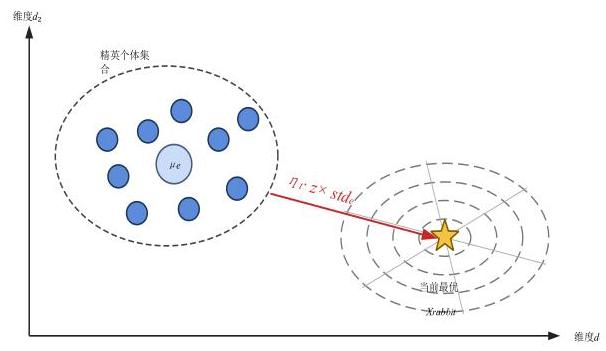
\includegraphics[width=0.8\linewidth]{figures/HHO/elite.jpg
    } % 调整宽度为适合您文档的值
    \caption{精英方差引导开发策略示意图}
    \label{fig:elite}
\end{figure}

首先,根据当前种群适应度值进行升序排序,选取前 $M$ 个个体构成精英子集,如下公式所示。
\begin{equation}
    M = \max \left( {2,\lceil {\rho N}\rceil }\right) \tag{24}
\end{equation}
其中, $\rho$ 为精英比例, $N$ 为种群规模。设精英子集为 $\varepsilon  = \left\{  {{X}_{1},{X}_{2},\ldots ,{X}_{M}}\right\}$ ,之后,进一步计算统计特征。对第 $\mathrm{d}$ 维而言, 精英个体的样本方差定义为:
\begin{equation}
    {\operatorname{var}}_{d} = \operatorname{Var}\left( {{X}_{1,d},{X}_{2,d},\cdots ,{X}_{M,d}}\right) ,\;d = 1,2,\cdots ,D \tag{25}
\end{equation}

之后, 得到精英子集的逐维标准差向量如下公式所示。
\begin{equation}
    {\text{ std }}_{e} = \sqrt{\text{ var } + \varepsilon } \tag{26}
\end{equation}

其中, $\varepsilon$ 为防止数值不稳定的微小常数。由此可见, ${st}{d}_{e}$ 能够反映精英个体在各维度上的离散程度,并可作为局部搜索步长的重要依据。
该策略主要作用于后期开发过程,当搜索进程进入后期,连续 $L$ 次更新未获得更优解时,启用精英方差引导开发策略。此时, 定义随迭代逐渐减小的步长因子为:
\begin{equation}
    {\eta }_{t} = {\eta }_{0} \times  \left( {1 - \frac{t}{T}}\right) \tag{27}
\end{equation}

其中, ${\eta }_{0}$ 为初始步长参数。
最后,以当前全局最优个体 ${X}_{\text{ rabbit }}$ 为中心,结合标准高斯随机向量 $\mathrm{z}$ 与精英逐维标准差向量 ${st}{d}_{e}$ ,构造局部开发候选解。如下公式所示：
\begin{equation}
    {X}_{\text{ cov }} = {X}_{\text{ rabbit }} + {\eta }_{t} \times  \left( {z \times  {\text{ std }}_{e}}\right) \tag{28}
\end{equation}
\subsection{时间复杂度分析}
算法的时间复杂度是评估其运行效率的关键指标。在时间复杂度方面，设种群规模为 $N$ ，问题维数为 $D$ ，最大函数评价次数为 $T$ 。对于所提出的改进哈里斯鹰优化算法 IHHO,初始化种群所需时间复杂度为 $\mathrm{O}\left( {ND}\right)$ ; 在迭代过程中,原始 HHO 位置更新、经验互益策略、 能量自适应 Cauchy-Gaussian 扰动策略以及精英方差引导开发策略均以向量逐维运算为主, 其单次更新复杂度可视为 $\mathrm{O}\left( D\right)$ ,因此累计复杂度约为 $\mathrm{O}\left( {TD}\right)$ 。此外,为构造精英子集,算法在每轮迭代中需对种群适应度进行排序, 该部分复杂度为 $\mathrm{O}\left( {N\log N}\right)$ 。在整个优化过程中累计可表示为 $\mathrm{O}\left( {{TN}\log N}\right)$ 。综合而言, $\mathrm{{IHHO}}$ 算法的总体时间复杂度可表示为 $\mathrm{O}\left( {{TD} + {TN}\log N}\right)$ 。考虑到连续优化问题中目标函数计算与位置更新通常占据主要计算成本，因此在实际应用中,算法的总体时间复杂度通常可近似看作 $\mathrm{O}\left( {TD}\right)$ 。
\subsection{算法实现}
该算法的操作流程可以总结为如下几步: :

步骤 1: 初始化种群, 计算种群适应度值, 确定全局最优个体, 同时保存初始历史经验信息并初始化个体停滞次数。

步骤 2: 用原始 HHO 的位置更新规则产生初始解集。

步骤 3：当搜索进程处于探索与开发衔接区间时，采用经验互益策略对历史有益经验进行继承与重组，生成经验互益候选解。

步骤 4: 根据实时得到的逃逸能量值, 用动态调整的 Cauchy-Gaussian 扰动机制产生候选解集来达到全局搜索和局部优化。

步骤 5：当算法进入后期阶段或个体出现连续停滞时，采用精英方差引导开发策略生成局部开发候选解。

步骤 6：对各候选解执行竞争选择并更新种群位置，随后更新历史经验库与停滞计数。若达到最大评价次数, 则输出全局最优解, 否则继续迭代。


\section{实验设计}


\subsection{基准函数对比实验}

\subsubsection{实验准备}
为了验证 IHHO 的优化效果，本小节选取了 CEC 2020 测试函数用于验证实验。哈里斯鹰优化算法 (Harris Hawks optimization, HHO) 、白鲸优化算法(Beluga Whale Optimization, BWO)、算术优化算法 (arithmetic optimization algorithm, AOA) 、正余弦优化算法(Sine Cosine Algorithm, SCA)和爬行动物搜索算法(Reptile Search Algorithm, RSA)作为对比实验。每个算法的种群个数 $N = {30}$ ，最大评价次数 T= $\dim  \times  {10000}$ 。这些算法的参数如表格 1 所示。
% CEC2020函数介绍
\begin{table}[ht]
\centering
\caption{Benchmark Functions Table}
\renewcommand{\arraystretch}{1.3} % 适当增加行高，视觉更舒适
\begin{tabularx}{\textwidth}{@{} l c X c @{}}
\toprule
\textbf{Category} & \textbf{No.} & \textbf{Functions} & \textbf{$F_i^* = F_i(x^*)$} \\ \midrule

Unimodal Function & 1 & Shifted and Rotated Bent Cigar Function (CEC 2017 F1) & 100 \\ \midrule

\multirow{3}{*}{Basic Functions} 
 & 2 & Shifted and Rotated Schwefel's Function (CEC 2014 F11) & 1100 \\
 & 3 & Shifted and Rotated Lunacek bi-Rastrigin Function (CEC 2017 F7) & 700 \\
 & 4 & Expanded Rosenbrock's plus Griewangk's Function (CEC 2017 $f_{19}$) & 1900 \\ \midrule

\multirow{3}{*}{Hybrid Functions} 
 & 5 & Hybrid Function 1 ($N = 3$) (CEC 2014 F17) & 1700 \\
 & 6 & Hybrid Function 2 ($N = 4$) (CEC 2017 F16) & 1600 \\
 & 7 & Hybrid Function 3 ($N = 5$) (CEC 2014 F21) & 2100 \\ \midrule

\multirow{3}{*}{Composition Functions} 
 & 8 & Composition Function 1 ($N = 3$) (CEC 2017 F22) & 2200 \\
 & 9 & Composition Function 2 ($N = 4$) (CEC 2017 F24) & 2400 \\
 & 10 & Composition Function 3 ($N = 5$) (CEC 2017 F25) & 2500 \\ \midrule

\multicolumn{4}{c}{\textbf{Search range: $[-100, 100]^D$}} \\ \bottomrule
\end{tabularx}
\end{table}

% 各算法参数设置表
\begin{table}[htbp]
\centering
\small
\caption{Parameter setting of each algorithm}
\begin{tabular}{ll}
\toprule
\textbf{Algorithms} & \textbf{Parameters} \\
\midrule
HHO & $S = 0.01$; $\beta = 1.5$ \\
BWO & $W_f \in [0.1, 0.05]$ \\
AOA & $C_1 = 0.2$; $C_3 = 3$; $\mu = 25$; $\sigma = 3$ \\
SCA & $C_1 \in [0,2]$; $C_2 \in [0,2]$; $C_3 \in [0,2]$ \\
RSA & $\alpha = 0.1$; $\beta = 0.005$; $S = 0.01$; $\beta = 1.5$ \\
IHHO & $ph = 0.85$; $L = 5$; $elite\_ratio = 0.2$; $\sigma_0 = 0.1$ \\
\bottomrule
\end{tabular}
\label{tb:each-alg-parameters}
\end{table}

\subsubsection{收敛曲线分析}
表格 2 是 6 种算法在 IEEE CEC 2020 独立运行 10 次获得的统计结果,其中维度 $\dim  = {10}$ 。从表 2 的分析可知，在 CEC 2020 标准测试函数集上 IHHO 算法的综合性能明显好于其它比较算法。在 CEC1 到 CEC8 以及 CEC5 和CEC6函数中, 该算法都取得了很好的均值性能, 很好地表现出了它对于不同类型连续优化问题的求解能力。 尤其是对于 CEC1、CEC5 和 CEC7 这类复杂的函数优化问题来说, IHHO 有着更为出色的表现, 它不但可以大幅度地降低求解过程中出现的误差, 而且还能有效地提升全局搜索能力以及鲁棒性, 这再一次表明它的高维非线性优化应用前景。从标准差结果来看, 采用 IHHO 算法处理的测试函数在各个维度上具有较好的一致性。其在 CEC2、CEC6、CEC8 和 CEC9 这些函数上标准差小, 说明该算法具有较好的鲁棒性。虽然 IHHO 标准差不是最小的, 在部分测试函数中, 但是其平均性能指标最好。相对于只对某些函数性能优越、而全局最优性能却不高, 其他的算法, IHHO 具有更好的综合优化能力。

原始 HHO 在解决复杂问题的时候虽然有它的优势, 但是它只用当前最好的个体和当前表现数据来更新位置, 没有利用历史的经验, 所以在多模态函数优化中容易造成种群多样性的下降以及后期收敛效果变差的现象。 BWO 在部分测试函数上表现出较好的性能, 但是在 CEC1、CEC5、CEC7 这些高维或者非线性搜索空间的函数中, 它的平均结果明显偏高, 说明这个算法对于这类搜索空间的适应能力较差, 容易陷入局部最优或者无法充分探索到搜索空间中的各个角落。AOA 比 IHHO、HHO 的算术运算驱动更新容易造成高维复杂场景下步长控制失衡而降低全局开发效率。SCA 有较强的探索性, 但是周期性的因子会对它的行为产生很大的影响, 造成后期搜索轨迹的起伏, 进而影响到收敛精度。RSA 在大多数测试函数中平均值、标准差都比其他方法高, 说明 RSA 对复杂的函数稳定性、鲁棒性不好，容易出现过早收敛和无效迭代。
综合评价结果表明, 在大多数测试函数中 IHHO 算法的性能最好, 说明本文所提出的改进方法是具有很强适用性和较大优化效果的。


\subsubsection{弗里德曼统计检验}

为了进一步探究不同算法在CEC 2020测试函数集中综合表现的好坏，本文用Friedman检验的方法对6种优化算法进行了多指标排名比较，具体的统计结果见表5。由表5可知，IHHO平均得分是1.43，在所有的评价指标下都居于第一的位置。该优异的成绩说明IHHO具有很强的局部搜索能力以及全局寻优稳定的特点，并且也显示出很强的普适性以及应用前景。
由各个函数的评价结果可知，IHHO在所有的CEC1-CEC8的函数里都名列前茅，在CEC9和CEC10中也有明显的优势。在CEC4函数上，各个算法的性能差异不大，平均值也很接近，但是IHHO依然保持较高的位置。这就说明CEC4函数对于算法综合性能的区分度低，对于整体排名的影响也小。根据IHHO多次任务表现出色以及稳定的平均排名结果，可以推测出该算法优异的原因是由算法的设计和优化机制所造成的。
相比于IHHO，原始HHO的总体表现虽然不是最好的，但是其平均性能仍然保持在一个较高的水平上，说明它有着比较好的基础结构。在历史经验迁移、自适应参数调节和后期改良这些地方，最初的HHO还存在着较大的提升之处。SCA、AOA的平均排名位于中间位置，说明它们在某些优化问题上具有一定的解题能力，但是并没有表现出很强的稳定性以及普适性，表现出的搜索机制对于问题类型适应性较低。BWO、RSA的表现也较低，特别是RSA，它在很多情况下都会出现测试函数中表现变坏的情况。根据Friedman检验统计分析结果可知，在综合性能上，IHHO比其它对比算法都要好。

% 各算法参数设置表
\begin{table}[htbp]
\centering
\small
\caption{Parameter setting of each algorithm}
\begin{tabular}{ll}
\toprule
\textbf{Algorithms} & \textbf{Parameters} \\
\midrule
HHO & $S = 0.01$; $\beta = 1.5$ \\
BWO & $W_f \in [0.1, 0.05]$ \\
AOA & $C_1 = 0.2$; $C_3 = 3$; $\mu = 25$; $\sigma = 3$ \\
SCA & $C_1 \in [0,2]$; $C_2 \in [0,2]$; $C_3 \in [0,2]$ \\
RSA & $\alpha = 0.1$; $\beta = 0.005$; $S = 0.01$; $\beta = 1.5$ \\
IHHO & $ph = 0.85$; $L = 5$; $elite\_ratio = 0.2$; $\sigma_0 = 0.1$ \\
\bottomrule
\end{tabular}
\label{tb:FriedmanX}
\end{table}
\subsection{特征选择应用}
\subsubsection{实验准备}
为进一步验证 IHHO 在高维特征选择问题中的有效性, 本文选取 8 个高维数据集进行了实验, 并从适应度值和分类准确率两个角度对算法性能进行评价。每个算法的评估次数为 1000 次。由表 6 可知, 在 Breast、CNS、 Leukemia 和 Leukemia\_3c 等数据集上, IHHO 的平均适应度值均取得最优或接近最优结果。在 Colon、Lung 和 Ovarian 等数据集, IHHO 也保持了较强竞争力。由表 7 可知, IHHO 在 Breast 和 CNS 数据集上取得了最高平均准确率, 在 Leukemia 和 Leukemia\_3c 数据集上准确率达到 1 , 表现出很强的分类能力。总体来看, IHHO 在多数数据集上实现了较低适应度值与较高准确率的统一, 说明其能够有效选择对分类任务更有贡献的特征子集。
从实证研究角度来说, IHHO 算法高维特征选择方面的好处就是同时具备筛选效率和分类成绩两个方面。它的筛选能力强, 适应度函数值越低, 所选出的特征子集对于分类器的性能提升就越大。通过各个数据集上的测试可知, IHHO 算法平均适应度比其它的对比方法要好, 说明 IHHO 算法对关键特征识别有较高的准确率和速度。分类任务上它所表现出的总效果和稳定程度更好一些。以 Breast、CNS、Leukemia 以及 Leukemia\_3c 等数据集为例, IHHO 不仅能取得较高的分类准确率, 而且能够得到低标准差的特征子集, 说明它所获得的特征子集有较好的重复验证性以及鲁棒性, 从而说明该算法对于实际应用是有可靠的、适用范围广的。

与之相对，在处理高维特征选择问题的时候，各个对比算法都存在一定的缺陷。原始 HHO 在一些数据集上接近 IHHO, 但是在 Leukemia\_3c、Breast、CNS 等数据集上的平均适应度比后者低得多, 说明它的优化精度仍然不够高, 在迭代后期很容易陷入局部最优解中。BWO 虽然在 Colon、Ovarian 数据集上表现出一定的优势, 但是整体性能波动较大, 说明该算法对于不同数据集的特性适应性不均衡, 不能形成稳定的算法性能。AOA 在大多数数据集中适应度值、分类准确率都比 IHHO 低很多, 说明它对于高维特征空间的探索比较粗放, 很难得到最佳的特征子集。SCA 在 Leukemia\_3c、Lung 数据集上表现比较好, 但是由于它周期性的搜索造成的稳定性问题, 在复杂的高维空间中很难得到长期的效果。RSA 在大部分的数据集上适应度值、分类准确率都处在较低的水平上, 说明该算法对高维特征选择的问题容易受到随机性的影响, 不能给出较好的筛选结果以及分类性能保证。

此外, 该方法对于所有数据集都不一定是最优的。在 Colon、Ovarian 数据集上, BWO 算法适应度函数值或者分类精确度稍微占优, 在 Lung 数据集中 HHO、SCA 的平均分类精度比 IHHO 高。因此, 在一定的数据分布下, 某些对比方法因为具有特有的更新方式而得到局部性的优势。对所有数据集的整体评价结果显示, IHHO 一般都会得到低适应度和高准确率, 或者近似的准确率, 表现出较强鲁棒性和较好的泛化性。根据以上分析可知, IHHO 对于高维特征的选择有较大的应用潜力和发展的空间。

\subsubsection{实验结果与分析}

从图 4 中可以看出, 使用了 8 个高维特征选取任务的数据集时, IHHO 算法具有较好的性能。相比起原始 HHO 算法, IHHO 有更快的收敛速度, 在大多数数据集中迭代次数比原始 HHO 算法要少很多, 并且适应度值也更低, 这就说明它的初始探索阶段更有较强的搜索能力, 后期优化过程中则更高效的收敛到目标。IHHO 的优化路径更平滑, 后期的波动小得多, 说明该种改进策略提高了全局搜索效率, 同时提高了局部区域的稳定性。 尤其对 Breast、CNS、Leukemia 和 Leukemia\_3c 这些有较高维度特征的数据集来说, IHHO 可以很快地达到较好的解, 并且保持低的适应度值, 说明该算法在高维空间中高效的全局搜索以及局部优化都有明显的优势。

相比于其它的对比算法, HHO 算法在收敛性能上有着明显的不足之处。虽然该算法已经有了比较完备的基础架构, 但是由于没有历史经验的继承方式以及自适应扰动控制策略, 在后期搜索时很容易出现收敛停滞、局部波动等状况。BWO 算法在某些数据集上能较快达到初步收敛的效果，但是由于搜索路径稳定性较差，容易受到随机扰动因素的影响，表现出曲线波动较大。AOA 算法虽然收敛速度比较慢，但是依靠迭代不断接近最优解的优势明显, 在大部分的应用场合中表现出较好的寻优能力。由于 SCA 算法更新规则存在较强的周期性约束, 造成数据集上产生明显的振荡现象, 从而对最后的解质量造成一定的影响。RSA 算法在整体收敛趋势上比较平缓，但是面对高维复杂的任务的时候会存在较差的鲁棒性，波动比较大。

从图 5 可以看出, IHHO 算法对大部分数据集的分类准确率都比较接近或者比最好的表现要好, 说明它的所选特征子集具有很强的判别性，可以更好地保留原始数据的核心信息。通过图 6 的分析可知，该算法分类性能好, 而且控制特征维度数量的效果不错。该结果说明该 IHHO 算法不仅可以提高分类的速度, 还可以很好地进行特征压缩、消除冗余。在有限特征下仍然能取得较高的分类准确率, 说明所选择的特征子集具有较好的泛化性能以及实际应用的价值。

根据图 4、图 5 和图 6 的结果可以发现, IHHO 的优势不仅仅在单个性能指标上体现出来, 而是在多个性能指标上的提高使得该算法的收敛性得到改善, 其稳定性也变好, 并且分类精度更高, 特征压缩能力也变强。相对于对比算法来说, IHHO 更快地确定出最优解区域, 在后期也会有较强的局部搜索能力, 而它提取出来的特征子集在分类性能和特征数量上表现得更好。这说明本文提出的改进策略能够有效提升哈里斯鹰优化算法在高维特征选择问题中的综合性能，使其在求解效率、结果质量和鲁棒性方面均优于原始 HHO 及其他对比算法。

\subsection{消融实验}

\subsection{参数敏感性实验}

\begin{table}[htbp]
  \centering
  \caption{IHHO算法参数敏感度正交实验方案表（$L_9(3^4)$）}
  \label{tab:orthogonal_test}
  \begin{tabular}{cccccc} % 6列居中对齐
    \toprule
    实验编号 & $ph$ & $L$ & $elite\_ratio$ & $\sigma_0$ & 测试指标 \\
    \midrule
    1 & 0.75 & 3 & 0.1 & 0.05 & 最优适应度/收敛迭代次数 \\
    2 & 0.75 & 5 & 0.2 & 0.1 & 最优适应度/收敛迭代次数 \\
    3 & 0.75 & 7 & 0.3 & 0.15 & 最优适应度/收敛迭代次数 \\
    4 & 0.85 & 3 & 0.2 & 0.15 & 最优适应度/收敛迭代次数 \\
    5 & 0.85 & 5 & 0.3 & 0.05 & 最优适应度/收敛迭代次数 \\
    6 & 0.85 & 7 & 0.1 & 0.1 & 最优适应度/收敛迭代次数 \\
    7 & 0.95 & 3 & 0.3 & 0.1 & 最优适应度/收敛迭代次数 \\
    8 & 0.95 & 5 & 0.1 & 0.15 & 最优适应度/收敛迭代次数 \\
    9 & 0.95 & 7 & 0.2 & 0.05 & 最优适应度/收敛迭代次数 \\
    \bottomrule
  \end{tabular}
\end{table}
\section{本章小结}
本章针对原始哈里斯鹰优化算法 (HHO) 易陷入局部最优、后期收敛精度不足等问题, 本文提出一种多策略改进的哈里斯鹰优化算法 (IHHO) 。算法从三个层面进行增强: 引入经验互益策略, 利用历史信息提升跳出局部最优的能力; 设计能量自适应 Cauchy-Gaussian 扰动策略, 根据逃逸能量动态平衡全局探索与局部开发; 提出精英方差引导开发策略，依据精英方差调整搜索步长，提高后期收敛精度。与其他先进算法比较，IHHO 在 Friedman 平均排名 1.43、收敛速度与鲁棒性上均显著优于对比算法。进一步地, 将 IHHO 应用于 8 个高维生物医学数据集的特征选择问题，其在多数数据集上取得了更低的分类错误率与更高的准确率，证明了其在特征筛选中的有效性。综上所述，IHHO 有效克服了原始算法的缺陷，在连续优化与高维特征选择中均表现出优越性能, 为相关优化问题提供了更高效的解决方案。
\chapter{总结与展望}

\section{全文总结}
本文针对高维医学数据集在处理过程中面临的特征维度高、计算资源消耗大、模型性能受冗余特征干扰等挑战，深入研究了元启发式算法在特征选择任务中的应用。通过对雾凇算法和哈里斯鹰优化算法的改进，提出了两种综合性能更优的算法，并验证了其在医学高维特征选择场景下的实用价值。主要研究工作总结如下：
\begin{enumerate}
\item 改进雾凇算法（IRIME）的提出与验证：针对原始雾凇算法（RIME）收敛速度慢、易陷入局部最优等问题，融合信息熵评估策略、拉格朗日插值法与随机重启机制构建 IRIME。信息熵评估策略通过动态特征加权增强种群多样性，拉格朗日插值法通过多项式逼近加速全局最优解收敛，随机重启机制有效避免早熟收敛。在 CEC 2017 基准函数测试中，IRIME 在 30 维和 50 维场景下的弗里德曼排名分别为 1.31 和 1.21，显著优于原始 RIME 及其他 7 种对比算法；在 12 个医学数据集（含 4 个高维数据集）的特征选择实验中，IRIME 在适应度值、分类准确率和特征子集精简度上均表现突出，尤其在 ALLAML 高维数据集上实现 100\% 分类准确率，验证了其在医学特征选择中的实用价值。
\item 改进哈里斯鹰优化算法（IHHO）的提出与验证：为解决原始哈里斯鹰优化算法（HHO）迭代中种群多样性下降、后期收敛精度不足等问题，设计融合多策略的 IHHO。引入经验互益策略整合历史搜索信息，提升跳出局部最优的能力；构建能量自适应柯西 - 高斯扰动策略，动态平衡全局探索与局部开发；提出精英方差引导开发策略，优化后期局部搜索精度。在 CEC 2020 基准函数测试中，IHHO 的弗里德曼平均排名达 1.43，优于原始 HHO 及 5 种经典群智能算法；在 8 个高维医学数据集的特征选择实验中，IHHO 在 Breast、CNS、Leukemia 等数据集上取得更低的平均适应度值和更高的分类准确率，部分数据集准确率达 100\%，所选特征子集兼具强判别性与泛化性，有效实现高维特征的精准筛选与冗余消除。
\item 核心技术贡献：本文通过多策略融合的设计思路，针对性解决了元启发式算法在医学高维特征选择中的核心痛点。两种改进算法均通过基准函数测试验证了优化性能的优越性，再通过真实医学数据集实验验证了实际应用价值，为医学高维数据的特征选择提供了两种可靠的技术方案，丰富了元启发式算法在生物医学领域的应用场景。
\end{enumerate}
% 在本文，我们提出了一种改进型 RIME 算法（IRIME），旨在解决原始 RIME 算法存在的局限性。具体而言，该改进方案通过整合三大核心创新机制实现性能突破：（1）信息熵评估策略通过量化搜索过程中的信息不确定性，动态平衡算法的探索（Exploration）与利用（Exploitation）能力，避免算法过早陷入局部最优或搜索效率低下的困境；（2）随机重启机制当算法检测到搜索进程陷入停滞状态时，自动触发随机初始化重启，重新开辟搜索路径，有效规避局部最优解的束缚；（3）拉格朗日插值法通过构建光滑的插值函数拟合搜索空间的目标函数分布，为算法提供更精准的搜索方向指引，从而显著提升收敛速度。此外，本文还提出了一种基于经验交流策略和 Q-learning 的改进哈里斯鹰优化算法（EES-HHO）。该算法通过经验匮乏、经验交叉和经验共享三个阶段的动态划分，有效平衡了种群的多样性和收敛性；同时引入 Q-learning 强化学习机制，使算法能够根据当前的搜索状态智能选择最优策略，进一步提升了算法在复杂优化问题上的适应性和鲁棒性。

% 为全面验证 IRIME 和 EES-HHO 算法的性能优势，我们在两大核心任务场景中开展了系统性实验：CEC 2017 基准测试集与特征选择任务。在 CEC 2017 测试集上，无论面对低维还是高维优化问题，IRIME 和 EES-HHO 均展现出卓越的全局优化能力不仅收敛速度远超原始算法及其他对比算法，还能获得更高的求解精度，充分验证了其在复杂优化场景中的适应性。在特征选择任务中，两种改进算法均能够精准识别数据集中的关键特征，有效剔除冗余信息，进而显著提升后续分类模型的性能；多组数据集上的实验结果均表明，其特征选择效果与分类精度均优于现有主流对比算法，凸显了算法在实际数据处理任务中的实用价值。

% 此外，我们通过消融实验（Ablation Studies）进一步验证了各项创新机制的有效性：单独移除任一机制后，算法的优化性能、收敛速度或特征选择精度均出现明显下降，而多种策略的有机结合则实现了出色的协同效应，显著增强了算法的整体性能。这一结果充分证明了各创新模块设计的合理性与必要性，为算法的后续改进提供了坚实的实验支撑。
\section{未来研究展望}
% 展望未来，相关研究可从两方面进一步推进：一方面，可通过优化算法的计算流程、引入并行计算等方式，进一步提升 IRIME 和 EES-HHO 的计算效率，以适应更大规模数据或更复杂优化问题的需求；另一方面，可探索融合更多先进搜索策略，拓展算法在多模态优化问题中的性能边界，此类问题因存在多个最优解而极具挑战性，本文提出的改进框架为相关研究提供了良好基础。同时，IRIME 和 EES-HHO 在工程实践中具有广阔的应用前景，尤其适用于图像处理（如图像分割、特征提取）、医疗诊断（如疾病风险预测、医学影像分析）等对优化精度与效率均有严格要求的领域。其高效处理优化问题与特征选择任务的双重能力，充分彰显了算法的通用性与实用价值，为解决实际工程中的复杂问题提供了新的技术思路。
尽管本文提出的 IRIME 和 IHHO 算法在医学数据集特征选择中取得了良好效果，但仍有进一步优化和拓展的空间，未来可从以下方向开展深入研究：

\begin{enumerate}
\item 算法性能的进一步优化：当前两种算法的改进策略虽已实现协同增效，但在超大规模医学数据集场景下，仍可能面临计算效率不足的问题。未来可探索引入代理模型技术，通过构建简化模型替代复杂的适应度函数计算，降低算法时间复杂度；同时，可研究自适应参数调节机制，减少算法对人工调参的依赖，提升其在不同类型医学数据集中的泛化能力。
\item 多目标特征选择模型的构建：现有研究主要聚焦于分类准确率最大化与特征维度最小化的单目标或复合目标优化，而医学特征选择实际还需考虑特征的临床可解释性、检测成本等多维度目标。未来可构建多目标优化框架，将临床实用性指标纳入目标函数，实现性能、效率、与实用性的多维度平衡，更好地满足临床实践需求。

\item 与深度学习模型的融合应用：当前算法主要与传统机器学习模型结合进行特征选择，未来可探索将改进算法与深度学习模型深度融合。一方面，利用元启发式算法优化深度学习模型的输入特征子集，降低模型训练成本；另一方面，可尝试将改进算法用于深度学习模型的超参数优化，实现特征选择与模型优化的协同，进一步提升医学数据处理的精度与效率。
\end{enumerate}

\newpage

\backmatter
\renewcommand{\chaptermark}[1]{\markboth{\songti #1}{}}
\makereferences
\newpage



% {
%     \appendix
%     \renewcommand{\chaptermark}[1]{\markboth{\heiti  附录\thechapter\ ~#1}{}}
%     \chapter{补充更多细节}

%     \section{补充图}
%     主要列入正文内过分冗长的公式推导，供查读方便所需的辅助性数学工具或表格；重复性数据图表；论文使用的缩写、程序全文及说明等。附录一般与论文全文装订在一起，与正文一起编页码，如果附录内容很多时可独立成册。若有多个附录按大写英文字母排序，如附录 A、附录B 等，每一个附录均另起一页。附录中的公式及图表编号也冠以附录序号字母加一短划线如公式A-2），图 A-2，表 B-2 等。本项可根据论文需要编排或省略。
%     \subsection{补充图}

%     \newclearpage
% }
% \ifdefined\blind  %这个if不要删除
%     % 盲审版没有致谢
% \else
%     \chapter{致谢}

%     四年时间转眼即逝，青涩而美好的本科生活快告一段落了。回首这段时间，我不仅学习到了很多知识和技能，而且提高了分析和解决问题的能力与养成了一定的科学素养。虽然走过了一些弯路，但更加坚定我后来选择学术研究的道路，实在是获益良多。这一切与老师的教诲和同学们的帮助是分不开的，在此对他们表达诚挚的谢意。

%     最后我要感谢我的家人，正是他们的无私的奉献和支持，我才有了不断拼搏的信心和勇气，才能取得现在的成果。

%     \vskip 108pt
%     \begin{flushright}
%         邱从波\makebox[1cm]{} \\
%         \today
%     \end{flushright}
%     \newpage
% \fi
% \chapter{攻读硕士学位期间取得的主要学术成果}

% \section*{1. 已发表的学术论文}
% 论文格式依照《温州大学研究生学位论文格式》（温州大学行政〔2016〕153号）文件要求，上传的盲审论文含封面（盲审格式）、中英文摘要和关键词、目录、正文、参考文献、注释、附录、攻读学位期间取得的研究成果（作者、发表卷期等信息一律用“XXX”替代，详见示例）,除去扉页、版权页、致谢等部分，论文封面及论文中不得出现温州大学、指导教师及作者等相关信息,一律用“***”替代。

% \ifdefined\blind  % 这个if不要删除
%     % 盲审版不透露自己姓名
%     \begin{enumerate}
%         \renewcommand{\labelenumi}{[\arabic{enumi}]}
%         \setlength{\itemindent}{0em}
%         \setlength{\labelsep}{0.5em}
  
%         \item XXX[J]. Journal of Materials Science-Materials in Electronics,2022,X(X): XXXX -XXXX.SCI收录，已发表，第三章的研究成果.
%         \item  XXX, XXX, XXX[J]. Journal of Physics: Conference Series.2021.X(X)(本人第一作者).EI收录，已发表，第四章的研究成果.
%     \end{enumerate}
% \else
%     攻读学位期间发表的学术论文目录格式同参考文献,并在最后注明刊物级别和第一完成单位名称。
%     \begin{enumerate}
%         \renewcommand{\labelenumi}{[\arabic{enumi}]}
%         \setlength{\itemindent}{0em}
%         \setlength{\labelsep}{0.5em}
  
%         \item Zhang X, Yu Z, Zhao L, et al. COMPrompter: reconceptualized segment anything model with multiprompt network for camouflaged object detection[J]. Science China Information Sciences, 2025, 68(1): 112104. JCR 一区， 温州大学.
%         \item Yu Z, Zhang X, Zhao L, et al. Exploring Deeper! Segment Anything Model with Depth Perception for Camouflaged Object Detection[C]//Proceedings of the 32nd ACM International Conference on Multimedia. 2024: 4322-4330. CCF-A ,温州大学.
%     \end{enumerate}
% \fi

% \section*{2. 参与的科研项目}


% \section*{3. 获奖情况}


%\newpage
\end{document}